\documentclass{../course_template/lectureClass}
%\usepackage{hyperref}
%\usepackage{svg}
%\usepackage{amsmath} % you need amsmath as the demo includes a use of \eqref
\makeglossaries
\begin{document}

%%%%%%%%%%%%%%%%%%%%%%%%%%%%%%%%%%%%%%%%%%%%%%%%%%%%%%%%%%%%%
%% Cover slide %%
%%%%%%%%%%%%%%%%%%%%%%%%%%%%%%%%%%%%%%%%%%%%%%%%%%%%%%%%%%%%%

\title[Power Electronics Devices]{Power Electronics Devices \\ (and Components)}
\author{Dr Bikash Sah}
\date{}
\begin{frame}[plain]
    \titlepage
\end{frame}

%%%%%%%%%%%%%%%%%%%%%%%%%%%%%%%%%%%%%%%%%%%%%%%%%%%%%%%%%%%%%
%% Outline / table of content %%
%%%%%%%%%%%%%%%%%%%%%%%%%%%%%%%%%%%%%%%%%%%%%%%%%%%%%%%%%%%%%
\begin{frame}{Content}
    \tableofcontents
\end{frame}

%%%%%%%%%%%%%%%%%%%%%%%%%%%%%%%%%%%%%%%%%%%%%%%%%%%%%%%%%%%%%
%% Lecture sections %%
%%%%%%%%%%%%%%%%%%%%%%%%%%%%%%%%%%%%%%%%%%%%%%%%%%%%%%%%%%%%%

%\includeonly{tex/Lecture01} % build only the specified file
%

\include{tex/Lecture01} % Overview / introduction
\include{tex/Lecture02} % Physics of basic semiconductor devices
\include{tex/Lecture03} % pn junctions and diodes
\include{tex/Lecture04} % Introduction to power semiconductor devices
\include{tex/Lecture05} % Conventional power semiconductor devices
\include{tex/Lecture06} % Wide bandgap power semiconductor devices
%\section{Passive components- Inductors and Capacitors}
\title[Passive components- Inductors and Capacitors]{Passive components- Inductors and Capacitors}  

\begin{frame}[plain]
    \titlepage
\end{frame}


%%%%%%%%%%%%%%%%%%%%%%%%%%%%%%%%%%%%%%%%%%%%%%%%%%%%%%%%%%%%%
%% Magnetic Concepts %%
%%%%%%%%%%%%%%%%%%%%%%%%%%%%%%%%%%%%%%%%%%%%%%%%%%%%%%%%%%%%%

%%%%%%%%%%%%%%%%%%%%%%%%%%%%%%%%%%%%%%%%%%%%%%%%%%%%%%%%%%%%%
%% Importance of Magnetics
%%%%%%%%%%%%%%%%%%%%%%%%%%%%%%%%%%%%%%%%%%%%%%%%%%%%%%%%%%%%%
\begin{frame}
\frametitle{Why are Magnetic Components Important in Power Electronics?}
Magnetic components are indispensable building blocks of almost every power electronic converter. Unlike semiconductor devices, which process electrical energy through switching action, magnetic components enable energy storage, energy transfer, filtering, isolation, and voltage conversion.

\begin{itemize}
    \item Inductors store energy in magnetic fields and control current ripple.
    \item Transformers transfer energy between circuits while providing galvanic isolation.
    \item Magnetic components determine:
    \begin{itemize}
        \item Converter efficiency,
        \item Power density,
        \item Thermal performance,
        \item Electromagnetic compatibility (EMC).
    \end{itemize}
    \item In modern GaN- and SiC-based converters, magnetics often become the primary bottleneck limiting switching frequency and power density.
\end{itemize}
\end{frame}

%%%%%%%%%%%%%%%%%%%%%%%%%%%%%%%%%%%%%%%%%%%%%%%%%%%%%%%%%%%%%
%% Classification
%%%%%%%%%%%%%%%%%%%%%%%%%%%%%%%%%%%%%%%%%%%%%%%%%%%%%%%%%%%%%
\begin{frame}
\frametitle{Classification of Magnetic Components}
Magnetic components used in power electronics can be broadly classified into two categories:

\vspace{0.2cm}

\begin{enumerate}
\item \textbf{Energy-transfer devices}
\begin{itemize}
\item Transfer energy from one electrical port to another.
\item Ideally store no energy.
\item Examples:
\begin{itemize}
\item Power transformers,
\item Current transformers (CTs),
\item Pulse transformers.
\end{itemize}
\end{itemize}

\item \textbf{Energy-storage devices}
\begin{itemize}
\item Store energy temporarily in magnetic fields.
\item Examples:
\begin{itemize}
\item Power inductors,
\item Coupled inductors,
\item Flyback transformers.
\end{itemize}
\end{itemize}

\end{enumerate}

\vspace{0.15cm}

This distinction is fundamental because the design objectives of inductors and transformers are significantly different.

\end{frame}


%%%%%%%%%%%%%%%%%%%%%%%%%%%%%%%%%%%%%%%%%%%%%%%%%%%%%%%%%%%%%
%% Ampere's circuital law: magnetic field strength %%
%%%%%%%%%%%%%%%%%%%%%%%%%%%%%%%%%%%%%%%%%%%%%%%%%%%%%%%%%%%%%
\begin{frame}
	\frametitle{Amp\`ere's circuital law: magnetic field strength}
	\begin{columns}
		\begin{column}{0.55\textwidth}
			Relates the circulation of a magnetic field around a closed loop to the electric current passing through the loop:
            \begin{align}
                \mbox{Integral form:} \quad &\oint_{\partial S} \bm{H} \cdot \mathrm{d}\bm{s} = I_{\mathrm{f}},\\
                \mbox{Differential form:} \quad &\nabla \times \bm{H} = \bm{J}_{\mathrm{f}}. 
                \label{eq:ampere_law}
            \end{align}
            Here, $\bm{H}$ is the magnetic field strength, $\bm{J}_{\mathrm{f}}$ is the free current density, and $I_{\mathrm{f}}$ is the free current enclosed by the loop $\partial S$. 
            \vspace{0.25cm}
            \begin{itemize}
                \item<2-> Free current: current that is not bound to a material (i.e., without polarization and magnetization currents).
                \item<3-> SI-units: $[H] = \si{\ampere\per\metre}$, $[J] = \si{\ampere\per\metre\squared}$
            \end{itemize}
		\end{column}
        \hfill
		\begin{column}{0.4\textwidth}
			\begin{figure}
				\centering
				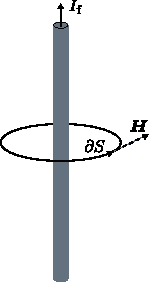
\includegraphics[height=0.7\textheight]{fig/lec07/Magnetic_field_strength_simple_conductor.pdf}
				\caption{Illustration of the magnetic field strength $\bm{H}$ around a simple conductor}
			\end{figure}
		\end{column}
		\end{columns}
\end{frame}


%%%%%%%%%%%%%%%%%%%%%%%%%%%%%%%%%%%%%%%%%%%%%%%%%%%%%%%%%%%%%
%% Ampere's circuital law: free current example %%
%%%%%%%%%%%%%%%%%%%%%%%%%%%%%%%%%%%%%%%%%%%%%%%%%%%%%%%%%%%%%
\begin{frame}
	\frametitle{Amp\`ere's circuital law: free current example}
	\begin{columns}
		\begin{column}{0.55\textwidth}
			What is the free current $I_{\mathrm{f}}$ enclosed by the loop $\partial S$?
            \begin{itemize}
                \item<2-> The current $I_1$ flows in the direction of the loop $\partial S$ (according to right-hand rule).
                \item<3-> The current $I_1$ must be counted $N$ times due to the $N$ turns of wire around the loop $\partial S$.
                \item<4-> The current $I_2$ flows in the opposite direction of the loop $\partial S$ (according to right-hand rule).
                \item<5-> Result:
            \end{itemize}
            \vspace{0.25cm}
            \onslide<5->{\begin{equation*}
                I_\mathrm{f} = N \cdot I_1 - I_2.
            \end{equation*}}
		\end{column}
        \hfill
		\begin{column}{0.45\textwidth}
			\begin{figure}
				\centering
				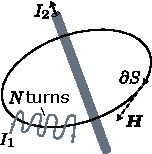
\includegraphics[height=0.5\textheight]{fig/lec07/Magnetic_field_strength_multiple_conductors.pdf}
				\caption{Arrangement with two electrical conductors}
			\end{figure}
		\end{column}
		\end{columns}
\end{frame}

%%%%%%%%%%%%%%%%%%%%%%%%%%%%%%%%%%%%%%%%%%%%%%%%%%%%%%%%%%%%%
%% Ampere's circuital law: simple solenoid  example%%
%%%%%%%%%%%%%%%%%%%%%%%%%%%%%%%%%%%%%%%%%%%%%%%%%%%%%%%%%%%%%
\begin{frame}
	\frametitle{Amp\`ere's circuital law: simple solenoid example}
	\begin{columns}
		\begin{column}{0.575\textwidth}
			Ampere's law for magnetic flux density $\bm{B}$ in vacuum:
            \begin{align}
                \mbox{Integral form:} \quad &\oint_{\partial S} \bm{B} \cdot \mathrm{d}\bm{s} = \mu_0 I,\\
                \mbox{Differential form:} \quad &\nabla \times \bm{B} = \mu_0\bm{J}. 
            \end{align}
            Here, $\mu_0$ is the permeability of free space, $\bm{J}$ is the total current density and $I$ is the total current enclosed by the loop $\partial S$. 
            \vspace{0.25cm}
            \begin{itemize}
                \item<2-> SI-unit: $[B] = \si{\tesla} = \si{\volt\second\per\metre\squared} = \si{\newton\per\ampere\per\metre}$
                \item<3-> Example contour $\partial S$  on the right covering $N$ turns and length $l$ (flux density within solenoid):
            \end{itemize}
            \onslide<4->{$$\oint_{\partial S} \bm{B} \cdot \mathrm{d}\bm{s} = N \mu_0 I  \Leftrightarrow B = \frac{N \mu_0 I}{l}$$}
		\end{column}
        \hfill
		\begin{column}{0.425\textwidth}
            \vspace{-0.2cm}
			\begin{figure}
				\centering
				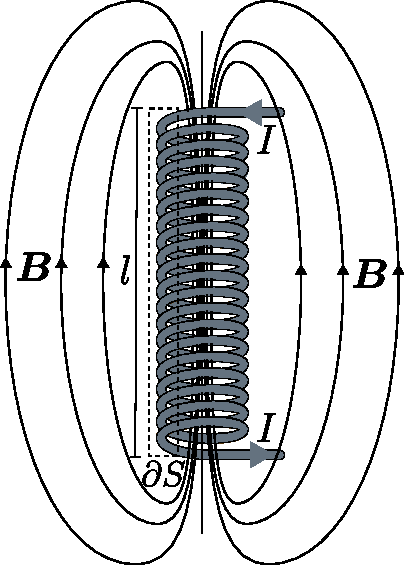
\includegraphics[height=0.68\textheight]{fig/lec07/Solenoid_Ampere_law.pdf}
				\caption{Magnetic flux density evaluated at the contour $\partial \bm{S}$  (adapted from: \href{https://commons.wikimedia.org/wiki/File:Solenoid_and_Ampere_Law.png}{Wikimedia Commons}, Goodphy, \href{https://creativecommons.org/licenses/by-sa/4.0/deed.en}{CC BY-SA 4.0})}
			\end{figure}
		\end{column}
		\end{columns}
\end{frame}

%%%%%%%%%%%%%%%%%%%%%%%%%%%%%%%%%%%%%%%%%%%%%%%%%%%%%%%%%%%%%
%% Shortcomings of the Ampere's circuital law %%
%%%%%%%%%%%%%%%%%%%%%%%%%%%%%%%%%%%%%%%%%%%%%%%%%%%%%%%%%%%%%
\begin{frame}
	\frametitle{Shortcomings of the Amp\`ere's circuital law}
	\begin{columns}
		\begin{column}{0.55\textwidth}
			Applying Amp\`ere's circuital law to a capacitor with a changing electric field $\bm{E}$ leads to a contradiction:
            \begin{itemize}
                \item Applying \eqref{eq:ampere_law} to $S_1$ yields:
                $$\oint_{\partial S_1} \bm{H} \cdot \mathrm{d}\bm{s} = I.$$
                \item<2-> In the case of $S_2$ we receive:
                $$\oint_{\partial S_2} \bm{H} \cdot \mathrm{d}\bm{s} = 0.$$
                \item<3-> However, both surfaces share the same bounding contour $\partial S$.
                \item<4-> Issue: The magnetic field strength $\bm{H}$ is not able to describe the displacement current.
            \end{itemize}
		\end{column}
        \hfill
		\begin{column}{0.45\textwidth}
			\begin{figure}
				\centering
				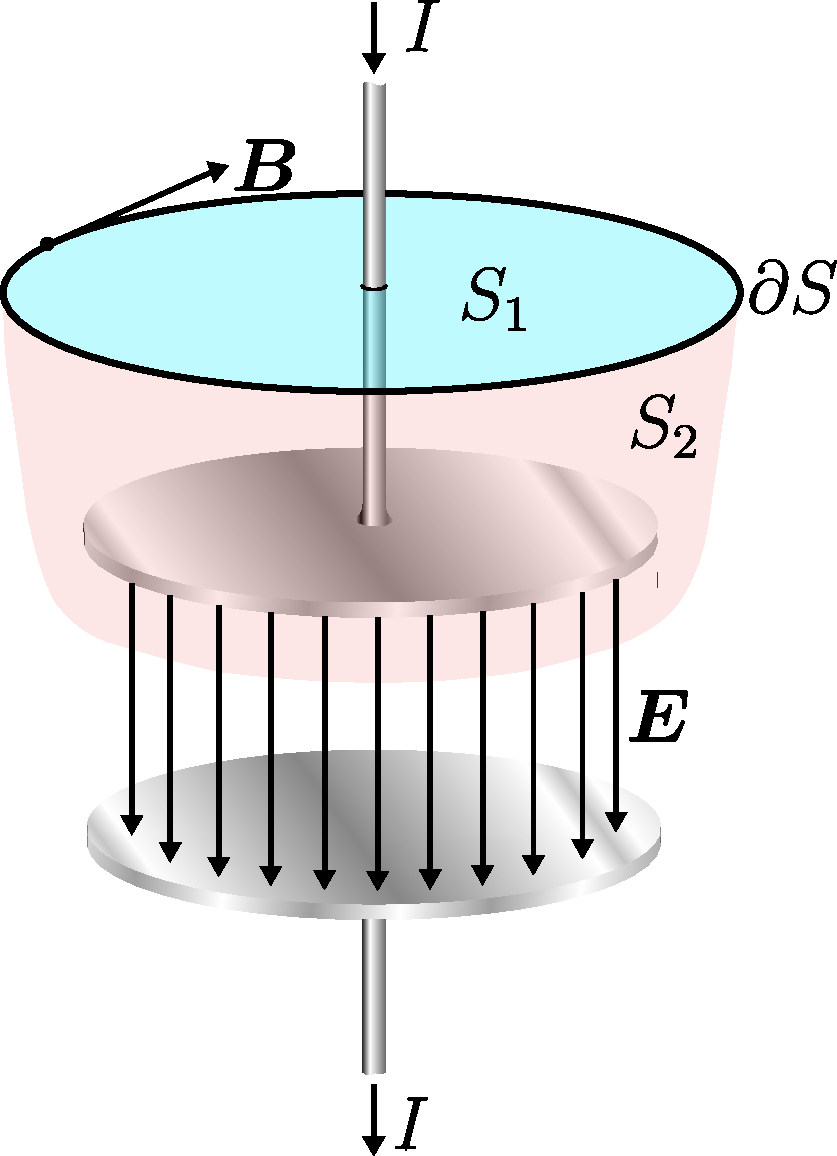
\includegraphics[height=0.55\textheight]{fig/lec07/Displacement_current_in_capacitor.pdf}
				\caption{Surfaces $S_1$ and $S_2$ share the same bounding contour $\partial S$. However, $S_1$ is pierced by conduction current, while $S_2$ is pierced by displacement current (adapted from: \href{https://commons.wikimedia.org/wiki/File:Displacement_current_in_capacitor.svg}{Wikimedia Commons}, public domain).}
			\end{figure}
		\end{column}
		\end{columns}
\end{frame}

%%%%%%%%%%%%%%%%%%%%%%%%%%%%%%%%%%%%%%%%%%%%%%%%%%%%%%%%%%%%%
%% Lorentz force %%
%%%%%%%%%%%%%%%%%%%%%%%%%%%%%%%%%%%%%%%%%%%%%%%%%%%%%%%%%%%%%
\begin{frame}
	\frametitle{Lorentz force}
    \begin{columns}
		\begin{column}{0.6\textwidth}
        The force $\bm{F}$ acting on a particle of electric charge $q$ with instantaneous velocity $\bm{v}$, due to an external electric field $\bm{E}$ and magnetic field $\bm{B}$, is given by
            \begin{equation}
                \bm{F} = q\left(\bm{E} + \bm{v}\times\bm{B}\right).
            \end{equation}
            \pause
            \begin{itemize}
                \item The term $q\bm{E}$  is called the electric force. \pause
                \item The term $q\left(\bm{v}\times\bm{B}\right)$ is called the magnetic force. \pause
                \item In Cartesian coordinates, the Lorentz force is given by:
            \end{itemize}
            \begin{equation}
                \begin{aligned}
                    F_x &= q\left(E_x + v_yB_z - v_zB_y\right),\\
                    F_y &= q\left(E_y + v_zB_x - v_xB_z\right),\\
                    F_z &= q\left(E_z + v_xB_y - v_yB_x\right).
                \end{aligned}
            \end{equation}
		\end{column}
        \hfill
		\begin{column}{0.40\textwidth}
			\begin{figure}
				\centering
				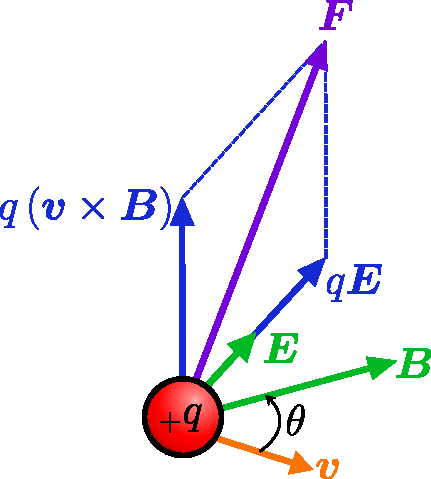
\includegraphics[height=0.5\textheight]{fig/lec07/Lorentz_force_particle.pdf}
				\caption{Lorentz force $\bm{F}$ on a particle (of charge $q$) in motion (instantaneous velocity $\bm{v}$) with given $\bm{E}$ and $\bm{B}$ fields (adapted from: \href{https://commons.wikimedia.org/wiki/File:Lorentz_force_particle.svg}{Wikimedia Commons}, Maschen, \href{https://creativecommons.org/publicdomain/zero/1.0/deed.en}{CC0})}
			\end{figure}
		\end{column}
		\end{columns}
\end{frame}

%%%%%%%%%%%%%%%%%%%%%%%%%%%%%%%%%%%%%%%%%%%%%%%%%%%%%%%%%%%%%
%% Hand rule of the magnetic Lorentz force %%
%%%%%%%%%%%%%%%%%%%%%%%%%%%%%%%%%%%%%%%%%%%%%%%%%%%%%%%%%%%%%
\begin{frame}
	\frametitle{Hand rule of the magnetic Lorentz force}
    \begin{figure}
        \centering
        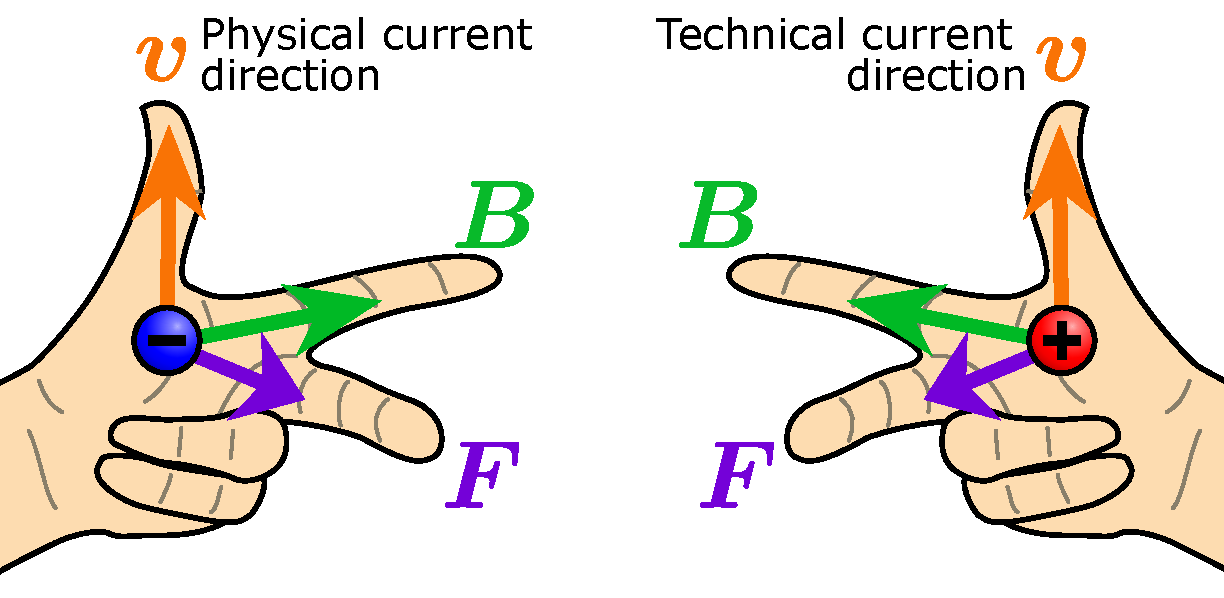
\includegraphics[height=0.6\textheight]{fig/lec07/Hand-rule-charges-both-hands.pdf}
        \caption{Right and left hand rule for the magnetic Lorentz force $q\left(\bm{v}\times\bm{B}\right)$ (adapted from: \href{https://commons.wikimedia.org/wiki/File:Right-hand-rule-charges-both-hands.svg}{Wikimedia Commons}, M. Run, \href{https://creativecommons.org/licenses/by-sa/3.0/deed.en}{CC BY-SA 3.0})}
    \end{figure}
\end{frame}

%%%%%%%%%%%%%%%%%%%%%%%%%%%%%%%%%%%%%%%%%%%%%%%%%%%%%%%%%%%%%
%% Lorentz force density for a continuous charge distribution %%
%%%%%%%%%%%%%%%%%%%%%%%%%%%%%%%%%%%%%%%%%%%%%%%%%%%%%%%%%%%%%
\begin{frame}
	\frametitle{Lorentz force density for a continuous charge distribution}
    \begin{columns}
		\begin{column}{0.5\textwidth}
         For a continuous charge distribution in motion, the Lorentz force density (force per unit volume) becomes: 
            \begin{equation}
                \bm{f} = \rho\bm{E} + \bm{J}\times\bm{B}.
            \end{equation}
            \begin{itemize}
                \item $\rho$ is the charge density (charge per unit volume).
                \item $\bm{J} = \rho \bm{v}$ is the current density.
            \end{itemize}
		\end{column}
        \hfill
		\begin{column}{0.5\textwidth}
			\begin{figure}
				\centering
				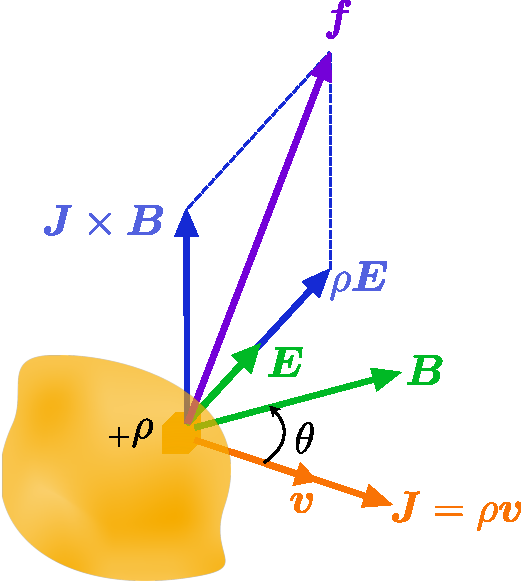
\includegraphics[height=0.6\textheight]{fig/lec07/Lorentz_force_continuum.pdf}
				\caption{Lorentz force density $\bm{f}$ on a continuous charge distribution (charge density $\rho$) in motion (adapted from: \href{https://commons.wikimedia.org/wiki/File:Lorentz_force_continuum.svg}{Wikimedia Commons}, Maschen, \href{https://creativecommons.org/publicdomain/zero/1.0/deed.en}{CC0})}
			\end{figure}
		\end{column}
		\end{columns}
\end{frame}

%%%%%%%%%%%%%%%%%%%%%%%%%%%%%%%%%%%%%%%%%%%%%%%%%%%%%%%%%%%%%
%% The Ampere--Maxwell equation %%
%%%%%%%%%%%%%%%%%%%%%%%%%%%%%%%%%%%%%%%%%%%%%%%%%%%%%%%%%%%%%
\begin{frame}
	\frametitle{The Amp\`ere -- Maxwell equation}
	\begin{columns}
		\begin{column}{0.6\textwidth}
			The charge of capacitor is:
            $$Q = \oint_{S_2} \bm{D}\cdot \mathrm{d}\bm{S}.$$
            \onslide<2->{If the electric field ($\bm{D} = \varepsilon_0\varepsilon_\mathrm{r} \bm{E}$) changes, a displacement current results:
            $$I_{\mathrm{d}} = \frac{\mathrm{d}}{\mathrm{d} t} \oint_{S_2} \bm{D}\cdot \mathrm{d}\bm{S}$$}
            \begin{itemize}
                \item<3-> Is not a classical electric current (moving charges) but a term to describe the changing electric field.
                \item<4-> Above, $\varepsilon_0$ is the vacuum permittivity and $\varepsilon_\mathrm{r}$ is the relative permittivity of a material.
            \end{itemize}
		\end{column}
        \hfill
		\begin{column}{0.4\textwidth}
			\begin{figure}
				\centering
				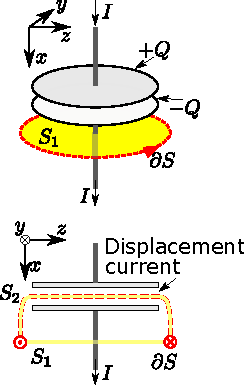
\includegraphics[height=0.65\textheight]{fig/lec07/Maxwell_integral_displacement_current.pdf}
				\caption{Illustration for calculating the displacement current (adapted from: \href{https://commons.wikimedia.org/wiki/File:Maxwell_integral_displacement_current.svg}{Wikimedia Commons}, public domain).}
			\end{figure}
		\end{column}
		\end{columns}
\end{frame}

%%%%%%%%%%%%%%%%%%%%%%%%%%%%%%%%%%%%%%%%%%%%%%%%%%%%%%%%%%%%%
%% The Ampere--Maxwell equation (cont.)%%
%%%%%%%%%%%%%%%%%%%%%%%%%%%%%%%%%%%%%%%%%%%%%%%%%%%%%%%%%%%%%
\begin{frame}
	\frametitle{The Amp\`ere -- Maxwell equation (cont.)}
        Adding the displacement current to \eqref{eq:ampere_law} we receive the Amp\`ere -- Maxwell equation:
            \begin{align}    
            \mbox{Integral form:} \quad  &\int_{\partial S} \bm{H} \cdot \mathrm{d}\bm{s} = \iint_{S}\left(\bm{J}_\mathrm{f} + \frac{\mathrm{d}}{\mathrm{d} t} \bm{D} \right)\cdot\mathrm{d}\bm{S}, \\
            \mbox{Differential form:} \quad &\nabla \times \bm{H} = \bm{J}_\mathrm{f} +  \frac{\partial\bm{D}}{\partial t}. 
            \label{eq:ampere_maxwell_law}
        \end{align}
        Above, $\bm{D}$ is the electric displacement field.
        \vspace{0.5cm}
        \begin{itemize}
            \item SI-unit: $[D] = \si{\coulomb\per\metre\squared}$
            \item SI-unit: $[E] = \si{\volt\per\metre}$
            \item $\varepsilon_0 \approx \SI{8.854e-12}{\farad\per\metre}$
        \end{itemize}
\end{frame}

%%%%%%%%%%%%%%%%%%%%%%%%%%%%%%%%%%%%%%%%%%%%%%%%%%%%%%%%%%%%%
%% Ampere's circuital law: magnetic flux %%
%%%%%%%%%%%%%%%%%%%%%%%%%%%%%%%%%%%%%%%%%%%%%%%%%%%%%%%%%%%%%
\begin{frame}
	\frametitle{Magnetic flux and flux linkage}
	\begin{columns}
		\begin{column}{0.575\textwidth}
			The magnetic flux $\phi$ is the surface integral of the normal component of $\bm{B}$ over that surface:
            \begin{align}
                \phi = \iint_{S} \bm{B} \cdot \mathrm{d}\bm{S}. 
            \end{align}
            \onslide<2->{As there are no magnetic monopoles, the magnetic flux through a closed surface (which is covering a volume without holes) is always zero:
            \begin{align}
                \oint_{S} \bm{B} \cdot \mathrm{d}\bm{S} = 0.
            \end{align}}
            \onslide<3->{The flux linkage $\psi$ is the product of the magnetic flux $\phi$ and the number of turns $N$ of a coil:
            \begin{align}
                \psi = N  \phi.
            \end{align}}
		\end{column}
        \hfill
		\begin{column}{0.425\textwidth}
            \vspace{-0.4cm}
			\begin{figure}
				\centering
				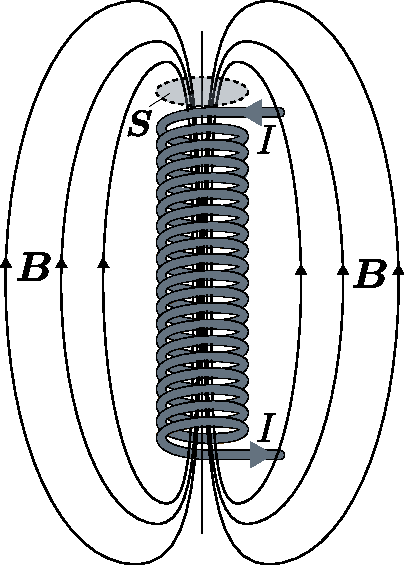
\includegraphics[height=0.68\textheight]{fig/lec07/Solenoid_Flux.pdf}
				\caption{Magnetic flux $\phi$ evaluated at the surface $\bm{S}$  (adapted from: \href{https://commons.wikimedia.org/wiki/File:Solenoid_and_Ampere_Law.png}{Wikimedia Commons}, Goodphy, \href{https://creativecommons.org/licenses/by-sa/4.0/deed.en}{CC BY-SA 4.0})}
                \label{fig:Solenoid_Flux}
			\end{figure}
		\end{column}
		\end{columns}
\end{frame}

%%%%%%%%%%%%%%%%%%%%%%%%%%%%%%%%%%%%%%%%%%%%%%%%%%%%%%%%%%%%%
%% Magnetic leakage flux %%
%%%%%%%%%%%%%%%%%%%%%%%%%%%%%%%%%%%%%%%%%%%%%%%%%%%%%%%%%%%%%
\begin{frame}
	\frametitle{Magnetic leakage flux}
	\begin{columns}
		\begin{column}{0.48\textwidth}
			\begin{itemize}
                \item In the scenarios with multiple coils, the magnetic flux generated by one coil will influence also the other coils.
                \item Exception: two coils are perfectly perpendicular to each other.
                \item However, the magnetic flux typically does not fully couple with the other coils
                \item The difference is the leakage flux $\phi_\sigma$.
            \end{itemize}
		\end{column}
        \hfill
		\begin{column}{0.48\textwidth}
            \vspace{-0.2cm}
			\begin{figure}
				\centering
				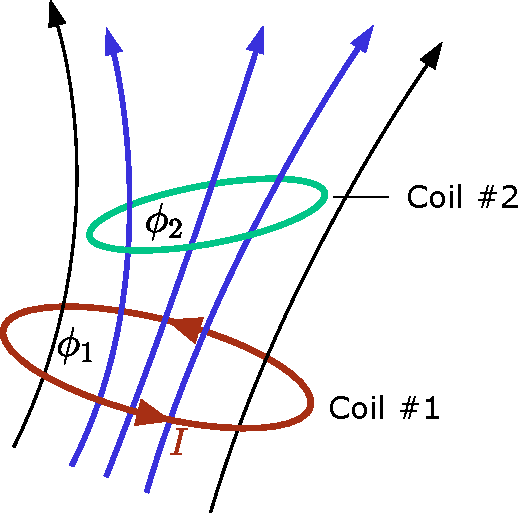
\includegraphics[height=0.55\textheight]{fig/lec07/Leakage_flux.pdf}
				\caption{The magnetic flux $\phi_1$ generated by the current $I$ does only partly couple with the second coil, while the difference $\phi_1-\phi_2$ is the leakage flux (adapted from: \href{https://commons.wikimedia.org/wiki/File:Mutual_Inductivity.svg}{Wikimedia Commons}, M. Wacenovsky, public domain)}
			\end{figure}
		\end{column}
		\end{columns}
\end{frame}


%%%%%%%%%%%%%%%%%%%%%%%%%%%%%%%%%%%%%%%%%%%%%%%%%%%%%%%%%%%%%
%% Leakage flux
%%%%%%%%%%%%%%%%%%%%%%%%%%%%%%%%%%%%%%%%%%%%%%%%%%%%%%%%%%%%%
\begin{frame}
    \frametitle{Magnetic leakage flux}
    \begin{columns}
        \begin{column}{0.58\textwidth}
            Not all magnetic flux generated by one winding links the other winding.
            \vspace{0.15cm}
            The uncoupled portion of flux is called leakage flux.
            \vspace{0.15cm}
            Leakage flux:
            \begin{itemize}
                \item Does not contribute to energy transfer.
                \item Produces voltage overshoot.
                \item Creates ringing during switching transitions.
                \item Becomes important at high switching frequencies.
            \end{itemize}
            \vspace{0.15cm}
            Leakage flux is inevitable in practical transformers.
        \end{column}
        \begin{column}{0.38\textwidth}
            \begin{figure}
                \centering
                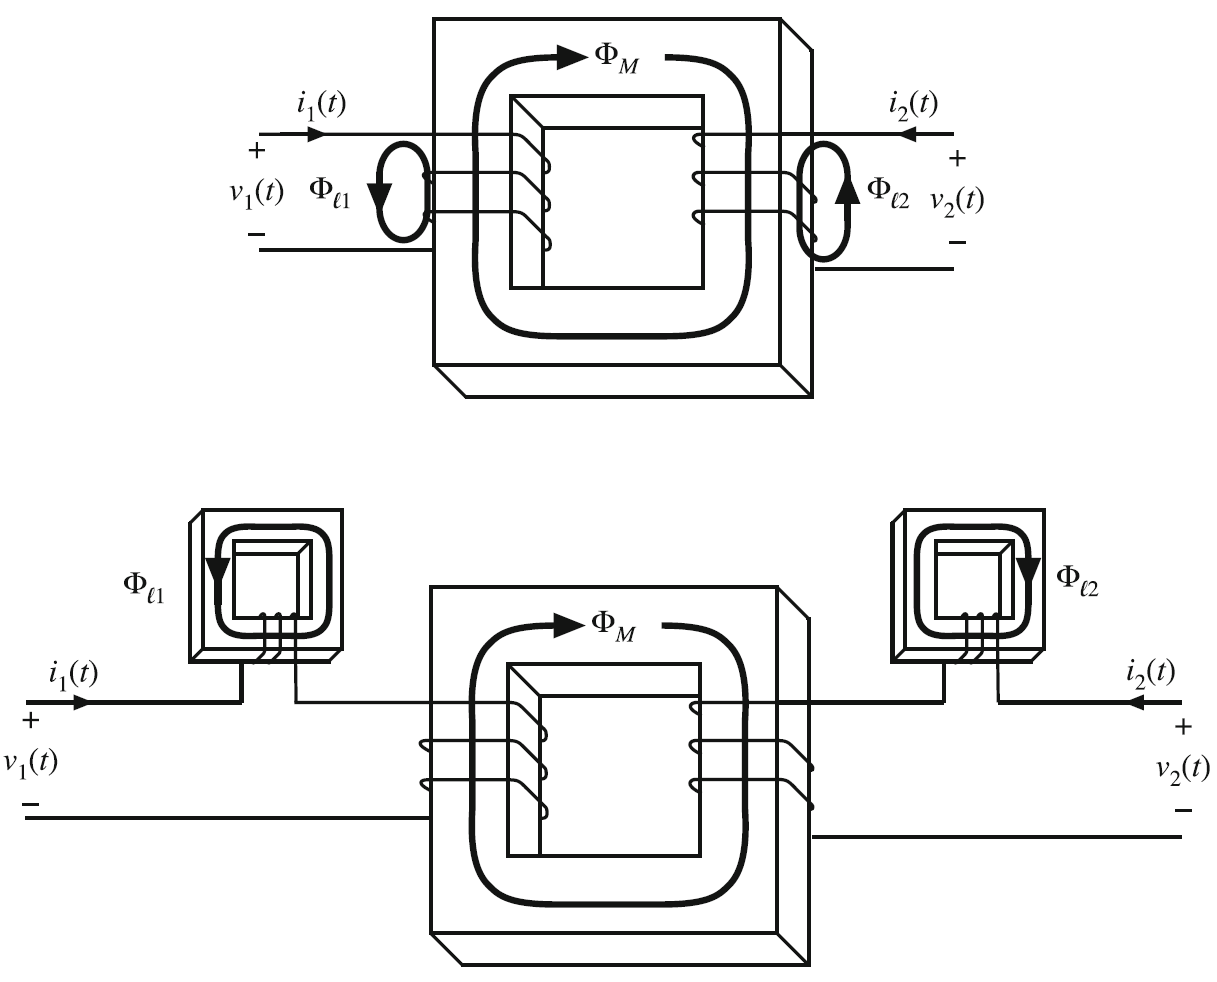
\includegraphics[width=\linewidth]{fig/lec07/Leakage_Flux.png}
                \caption{Leakage-flux paths that do not couple both windings. Adapted from Erickson and Maksimovic, \textit{Fundamentals of Power Electronics}, 3rd edition, Springer, 2013.}
            \end{figure}
        \end{column}
    \end{columns}
\end{frame}


%%%%%%%%%%%%%%%%%%%%%%%%%%%%%%%%%%%%%%%%%%%%%%%%%%%%%%%%%%%%% %% Lenz's law %%%%%%%%%%%%%%%%%%%%%%%%%%%%%%%%%%%%%%%%%%%%%%%%%%%%%%%%%%%%%
\begin{frame} 
    \frametitle{Lenz's Law: Direction of Induced Voltage and Current} 
    \begin{columns} 
        \begin{column}{0.58\textwidth} 
            Lenz's law defines the polarity of the induced voltage. The induced current always acts in a direction that opposes the change in magnetic flux that produced it. 
            \vspace{0.2cm} 
            \begin{itemize} 
                \item If the original flux increases, the induced current produces an opposing flux. 
                \item If the original flux decreases, the induced current tries to maintain it. 
                \item This is a direct consequence of energy conservation. 
                \item Lenz's law explains eddy currents, transformer action, leakage effects, and magnetic damping. 
            \end{itemize} 
            \vspace{0.2cm} 
            For a shorted conducting loop, 
            \begin{align} v_{\mathrm{ind}}(t)=\frac{d\Phi(t)}{dt}, \qquad i_{\mathrm{ind}}(t)=\frac{v_{\mathrm{ind}}(t)}{Z_{\mathrm{loop}}} 
            \end{align} The induced current produces a secondary flux that opposes the original flux variation. 
        \end{column} 
        \begin{column}{0.38\textwidth} 
            \begin{figure} 
                \centering 
                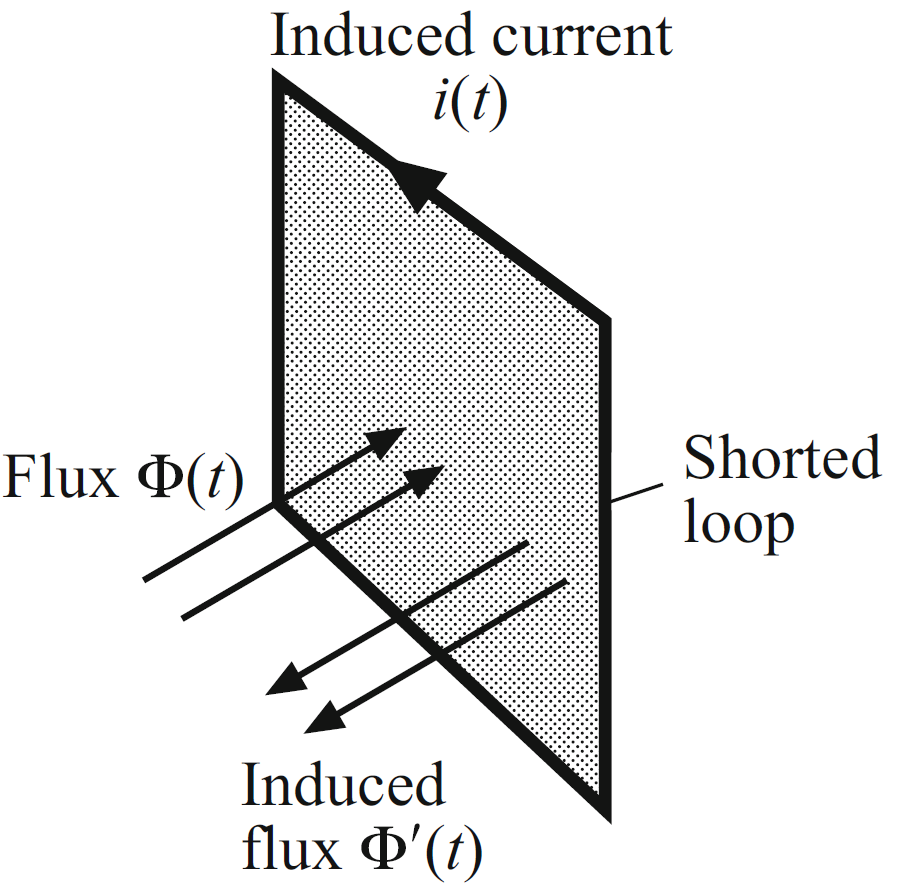
\includegraphics[width=0.75\linewidth]{fig/lec07/Lenz_law.png} 
                \caption{Lenz's law in a shorted loop: the induced current produces flux opposing the applied flux variation. Adapted from Erickson and Maksimovic, \textit{Fundamentals of Power Electronics}, 3rd edition, Springer, 2013.}
            \end{figure} 
        \end{column} 
    \end{columns} 
\end{frame}




%%%%%%%%%%%%%%%%%%%%%%%%%%%%%%%%%%%%%%%%%%%%%%%%%%%%%%%%%%%%%
%% Inductance %%
%%%%%%%%%%%%%%%%%%%%%%%%%%%%%%%%%%%%%%%%%%%%%%%%%%%%%%%%%%%%%
\begin{frame}
	\frametitle{Inductance}
	The inductance $L$ describes the ratio between the magnetic flux linkage $\psi(t)$ to the current $i(t)$:
    \begin{align}
        \psi(t) = L i(t).
    \end{align}
    \pause
    \textbf{Example}:  From the solenoid in \figref{fig:Solenoid_Flux} we know that the magnetic flux linkage $\psi$ is:
    $$\psi = N \iint_{S} \bm{B} \cdot \mathrm{d}\bm{S}= \frac{1}{l}N^2 \mu_0 I \pi r^2 $$
    with $r$ being the radius of the solenoid. \pause Hence, the inductance $L$ is:
    $$L = \frac{\psi}{I} = \frac{N^2 \mu_0 \pi r^2}{l}.$$
    \begin{itemize}
        \item SI-unit: $[L] = \si{\henry} = \si{\volt\second\per\ampere}$
        \item The inductance is an important parameter describing inductive systems.
    \end{itemize}
\end{frame}

%%%%%%%%%%%%%%%%%%%%%%%%%%%%%%%%%%%%%%%%%%%%%%%%%%%%%%%%%%%%%
%% Self and mutual inductance %%
%%%%%%%%%%%%%%%%%%%%%%%%%%%%%%%%%%%%%%%%%%%%%%%%%%%%%%%%%%%%%
\begin{frame}
	\frametitle{Self and mutual inductance}
    \begin{columns}
		\begin{column}{0.45\textwidth}
            Based on the inductive coupling between the two coils from \figref{fig:Transformer3d_col3}, we can define the magnetic flux matrix:
            \begin{equation}
                \bm{\phi} = \begin{bmatrix} \phi_{11} & \phi_{12} \\ \phi_{21} & \phi_{22} \end{bmatrix} .
                \label{eq:flux_matrix_transformer}
            \end{equation}
            \vspace{-0.2cm}
			\begin{itemize}
                \item<2-> $\phi_{11}$: magnetic flux component of coil 1 due to its own current $i_1$
                \item<3-> $\phi_{12}$: magnetic flux component of coil 1 due to the current $i_2$ in coil 2
                \item<4-> $\phi_{21}$: magnetic flux component of coil 2 due to the current $i_1$ in coil 1
                \item<5-> $\phi_{22}$: magnetic flux component of coil 2 due to its own current $i_2$
            \end{itemize}
		\end{column}
        \hfill
		\begin{column}{0.525\textwidth}
			\begin{figure}
				\centering
				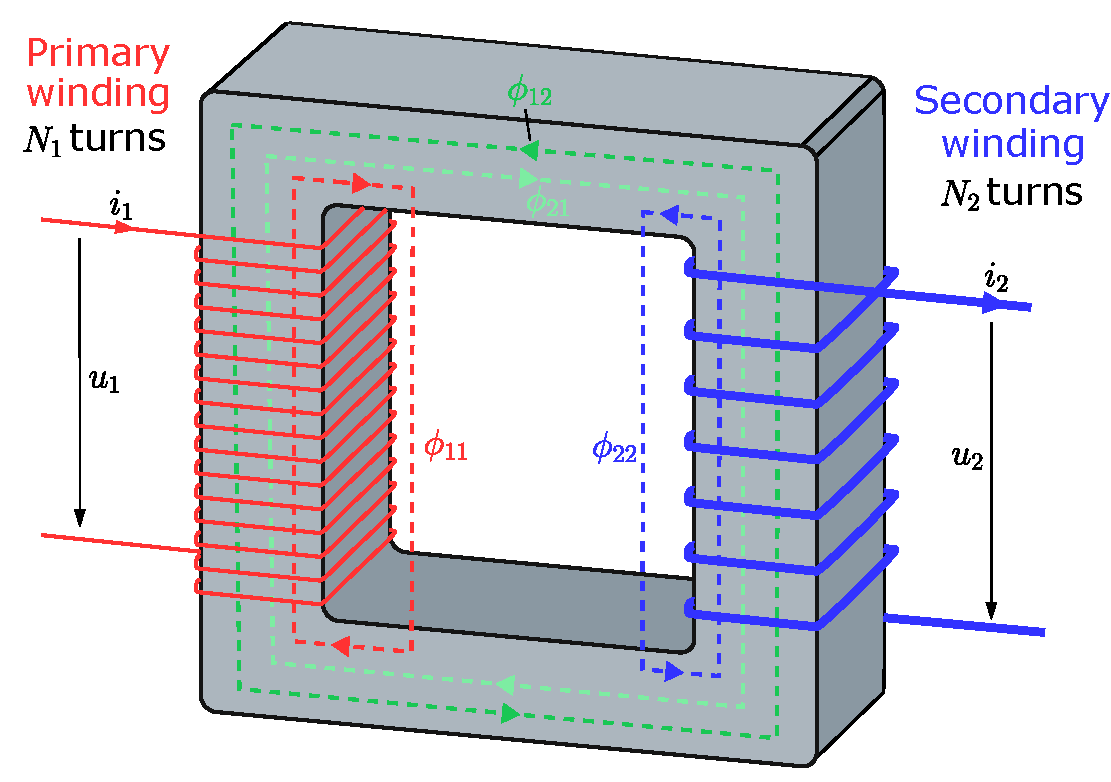
\includegraphics[height=0.575\textheight]{fig/lec07/Transformer3d_col3.pdf}
				\caption{Two coils coupled via a common core (adapted from: \href{https://commons.wikimedia.org/wiki/File:Transformer3d_col3.svg}{Wikimedia Commons}, Bill C., \href{https://creativecommons.org/licenses/by-sa/3.0/deed.en}{CC~BY-SA~3.0})}
                \label{fig:Transformer3d_col3}
			\end{figure}
		\end{column}
		\end{columns}
\end{frame}

%%%%%%%%%%%%%%%%%%%%%%%%%%%%%%%%%%%%%%%%%%%%%%%%%%%%%%%%%%%%%
%% Self and mutual inductance (cont.) %%
%%%%%%%%%%%%%%%%%%%%%%%%%%%%%%%%%%%%%%%%%%%%%%%%%%%%%%%%%%%%%
\begin{frame}
	\frametitle{Self and mutual inductance (cont.)}
    Utilizing the permeance definition (``magnetic conductance'') 
    \begin{equation}
        \Lambda = \frac{\phi}{N i},
    \end{equation}
    \pause
    we can represent \eqref{eq:flux_matrix_transformer} as:
    \begin{equation}
        \phi_{11} = \Lambda_{11} N_1 i_1, \quad \phi_{12} = \Lambda_{12} N_2 i_2, \quad \phi_{21} = \Lambda_{21} N_1 i_1, \quad \phi_{22} = \Lambda_{22} N_2 i_2.
    \end{equation}
    \pause
    The resulting flux linkage per coil is then:
    \begin{equation}
        \begin{alignedat}{3}
        \psi_1 &= N_1\left(\phi_{11} + \phi_{21} + \phi_{12}\right), \quad && \psi_2 && =  N_2\left(\phi_{22} + \phi_{12} + \phi_{21}\right),\\ \pause
               &=\underbrace{\left(\Lambda_{11}N_1^2+\Lambda_{21}N_1^2\right)}_{L_1}i_1 + \underbrace{\Lambda_{12}N_1N_2}_{M_{12}}i_2, \quad && && =\underbrace{\left(\Lambda_{22}N_2^2+\Lambda_{12}N_1^2\right)}_{L_2}i_2 + \underbrace{\Lambda_{21}N_1N_2}_{M_{21}}i_1. 
        \end{alignedat}
        \label{eq:flux_linkage_transformer}
    \end{equation}
    Above, $L_1$ and $L_2$ are the self-inductances, $M_{12}$ and $M_{21}$ are the mutual inductances.
\end{frame}

%%%%%%%%%%%%%%%%%%%%%%%%%%%%%%%%%%%%%%%%%%%%%%%%%%%%%%%%%%%%%
%% Self and mutual inductance (cont.) %%
%%%%%%%%%%%%%%%%%%%%%%%%%%%%%%%%%%%%%%%%%%%%%%%%%%%%%%%%%%%%%
\begin{frame}
	\frametitle{Self and mutual inductance (cont.)}
    Hence, we can define the flux linkages of both coils using the following inductance matrix:
    \begin{equation}
        \bm{\psi} = \begin{bmatrix} \psi_1 \\ \psi_2 \end{bmatrix} = \begin{bmatrix} L_1 & M_{12} \\ M_{21} & L_2 \end{bmatrix} \begin{bmatrix} i_1 \\ i_2 \end{bmatrix} = \bm{L}\bm{i}.
        \label{eq:flux_linkage_matrix_transformer}
    \end{equation}
    \pause
    Due to the symmetry of the inductive coupling, the mutual inductances are identical:
    \begin{equation}
        M_{12} = M_{21} = M.
    \end{equation}
    \pause
    Based on \eqref{eq:flux_linkage_transformer}, we can also split the self-inductance $L_i$ of the $i$-th coil into the sum of the leakage inductance $L_{i,\sigma}$ and the magnetizing inductance $L_{i,\mathrm{m}}$:
    \begin{equation}
        L_i = L_{i,\sigma} + L_{i,\mathrm{m}} = \Lambda_{ii}N_i^2 + \Lambda_{ji}N_i^2 \quad \mbox{with} \quad i \neq j. 
        \label{eq:inductance_split}
    \end{equation}
    \pause
    Finally, we can define the coupling coefficient $k$ as:
    \begin{equation}
        k = \frac{M}{\sqrt{L_1 L_2}}, \qquad 0 \leq k \leq 1,
        \label{eq:coupling_coefficient}
    \end{equation}
    which indicates how strong or week the inductive coupling between the coils is.
\end{frame}


%%%%%%%%%%%%%%%%%%%%%%%%%%%%%%%%%%%%%%%%%%%%%%%%%%%%%%%%%%%%%
%% Leakage inductance
%%%%%%%%%%%%%%%%%%%%%%%%%%%%%%%%%%%%%%%%%%%%%%%%%%%%%%%%%%%%%
\begin{frame}
    \frametitle{Leakage Inductance}
    \begin{columns}
        \begin{column}{0.58\textwidth}
            The energy associated with leakage flux is represented electrically as leakage inductance.
            \vspace{0.15cm}
            Leakage inductance appears in series with the transformer windings.
            \vspace{0.15cm}
            Consequences include:
            \begin{itemize}
                \item Reduced transient response
                \item Increased switching stress
                \item Voltage spikes
                \item Resonant ringing
            \end{itemize}
            \vspace{0.15cm}
            In resonant converters, however, leakage inductance can be deliberately utilized as a functional circuit element.
        \end{column}
        \begin{column}{0.38\textwidth}
            \begin{block}{Design Objective}
                Conventional transformer:
                \begin{equation}
                    L_{lk}
                    \rightarrow
                    \mathrm{minimum}
                \end{equation}
                \vspace{0.15cm}
                LLC converter:
                \begin{equation}
                    L_{lk}
                    \rightarrow
                    \mathrm{useful}
                \end{equation}
            \end{block}
        \end{column}
    \end{columns}
\end{frame}


%%%%%%%%%%%%%%%%%%%%%%%%%%%%%%%%%%%%%%%%%%%%%%%%%%%%%%%%%%%%% %% Electrical and magnetic domains %%%%%%%%%%%%%%%%%%%%%%%%%%%%%%%%%%%%%%%%%%%%%%%%%%%%%%%%%%%%%
\begin{frame} 
\frametitle{Interaction Between Electrical and Magnetic Domains} \begin{columns} 
    \begin{column}{0.57\textwidth} 
        A magnetic component is an energy-processing interface between the electrical and magnetic domains. 
        \vspace{0.2cm} In the electrical domain, 
        \begin{align} p_e(t)=v(t)i(t) 
        \end{align} In the magnetic domain, the corresponding variables are MMF and rate of change of flux: 
        \begin{align} 
            p_m(t)=F(t)\frac{d\Phi(t)}{dt} 
        \end{align} Using Amp\`ere's and Faraday's laws, 
        \begin{align} 
            v(t)i(t) = Ni(t)\frac{d\Phi(t)}{dt} = F(t)\frac{d\Phi(t)}{dt} 
        \end{align} 
        \begin{itemize} 
            \item Voltage corresponds to flux rate. 
            \item Current corresponds to magneto-motive force. 
            \item Energy transfer occurs through magnetic field coupling. 
        \end{itemize} 
    \end{column} 
    \begin{column}{0.39\textwidth} 
        \begin{figure} 
            \centering 
            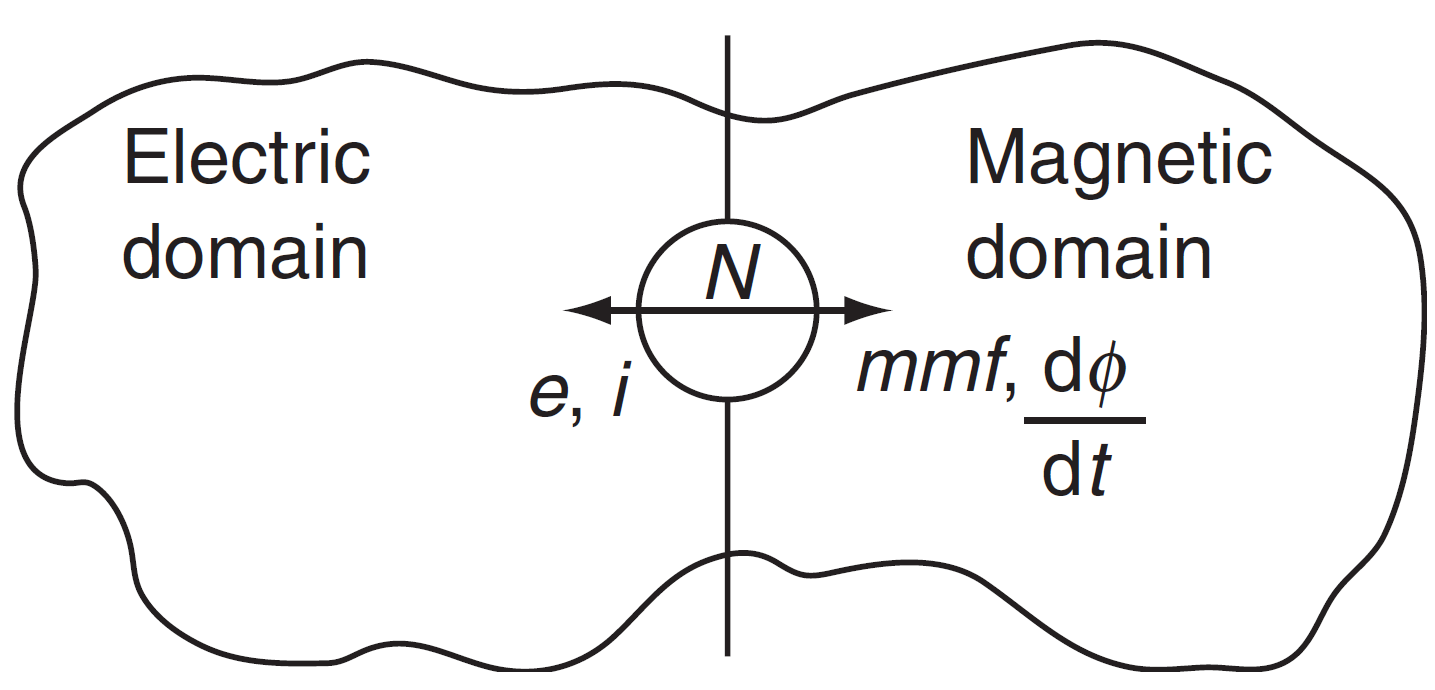
\includegraphics[width=\linewidth]{fig/lec07/electric_magnetic_domains.png} 
            \caption{Interaction between electric and magnetic domains. Adapted from Umanand, \textit{Power Electronics: Essentials and Applications}, 2nd edition, Wiley, 2012.}
        \end{figure} 
    \end{column} 
\end{columns} 
\end{frame}


%%%%%%%%%%%%%%%%%%%%%%%%%%%%%%%%%%%%%%%%%%%%%%%%%%%%%%%%%%%%% %% Electrical magnetic analogy %%%%%%%%%%%%%%%%%%%%%%%%%%%%%%%%%%%%%%%%%%%%%%%%%%%%%%%%%%%%%
\begin{frame} 
    \frametitle{Electrical--Magnetic Domain Analogy} 
    \begin{columns} 
        \begin{column}{0.56\textwidth} 
            The magnetic domain can be understood using analogies with electrical circuits. This is extremely useful for designing inductors and transformers. 
            \vspace{0.15cm} 
            \begin{table} 
                \centering 
                \small 
                \begin{tabular}{lll} 
                    \hline 
                    \textbf{Electrical} & \textbf{Magnetic} & \textbf{Meaning}\\ \hline 
                    Voltage $v$ & MMF $F$ & Driving effort\\ 
                    Current $i$ & Flux $\Phi$ & Flow quantity\\ 
                    Resistance $R$ & Reluctance $\mathcal{R}$ & Opposition to flow\\ 
                    Conductance $G$ & Permeance $\Lambda$ & Ease of flow\\ 
                    Current density $J$ & Flux density $B$ & Flow per area\\ 
                    Electric field $E$ & Magnetic field $H$ & Field intensity\\ 
                    \hline 
                \end{tabular} 
            \end{table} 
            \vspace{0.15cm} 
            The most important analogy is: 
            \begin{align} 
                V=IR \qquad \Longleftrightarrow \qquad F=\Phi\mathcal{R} 
            \end{align} 
        \end{column} 
        \begin{column}{0.40\textwidth} 
            \begin{block}{Design Interpretation} 
                \small A magnetic core behaves like a path for magnetic flux. A high-permeability core provides a low-reluctance path, just as a low-resistance conductor provides an easy path for electric current. 
            \end{block} 
            \vspace{0.2cm} 
            \begin{itemize} 
                \small 
                \item Air gaps increase reluctance. 
                \item Larger core area reduces reluctance. 
                \item Longer magnetic paths increase reluctance. 
                \item High permeability reduces reluctance. 
            \end{itemize} 
            \vspace{0.15cm}
        \end{column} 
    \end{columns} 
\end{frame}


%%%%%%%%%%%%%%%%%%%%%%%%%%%%%%%%%%%%%%%%%%%%%%%%%%%%%%%%%%%%% %% Flux and flux density %%%%%%%%%%%%%%%%%%%%%%%%%%%%%%%%%%%%%%%%%%%%%%%%%%%%%%%%%%%%%
\begin{frame} 
    \frametitle{Magnetic Flux and Flux Density} 
    \begin{columns} 
        \begin{column}{0.5\textwidth} 
            Magnetic flux $\Phi$ represents the total magnetic field passing through a given surface. Flux density $B$ represents how concentrated this flux is within the core cross-section. 
            \begin{align} 
                \Phi=\int_S \mathbf{B}\cdot d\mathbf{A} 
            \end{align} 
            For uniform flux density, 
            \begin{align} 
                \Phi=BA_c 
            \end{align} 
            \begin{align} 
            \text{Hence,} B=\frac{\Phi}{A_c} 
            \end{align} 
            where $A_c$ is the cross-sectional area of the magnetic core.
        \end{column} 
        \begin{column}{0.5\textwidth} 
            \vspace{-1.2cm}
            \begin{figure} 
                \centering 
                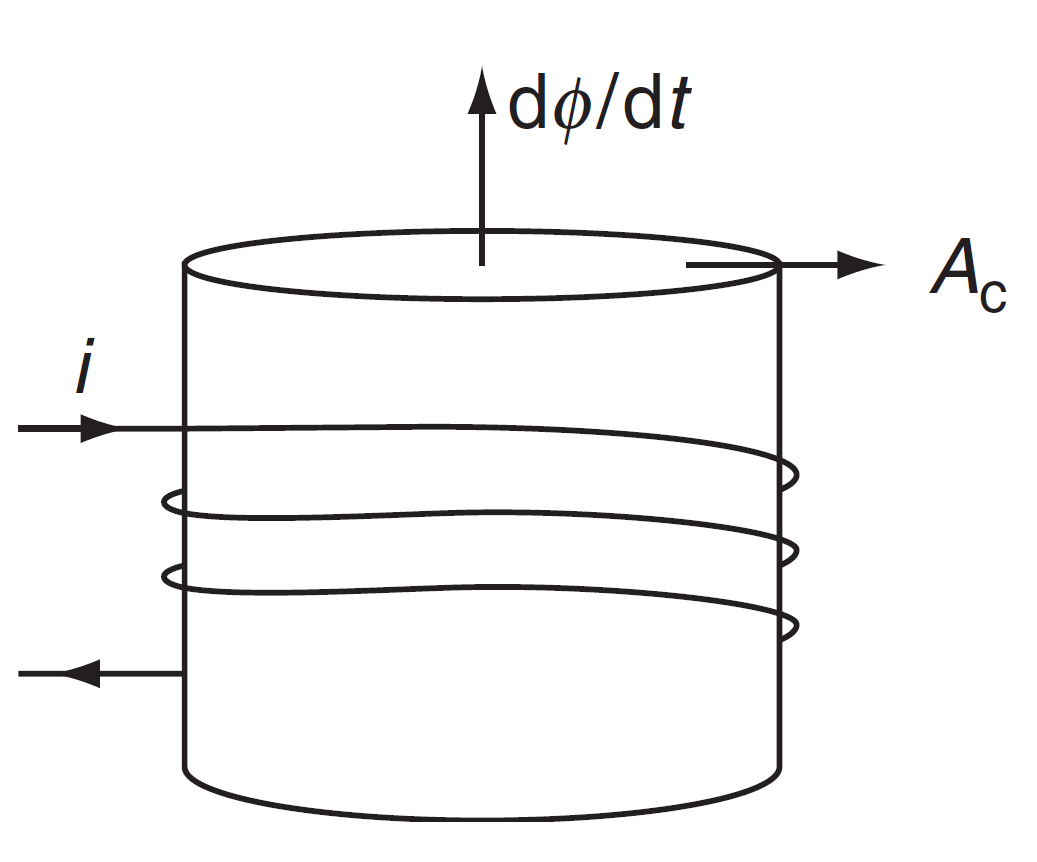
\includegraphics[width=0.5\textwidth]{fig/lec07/flux_density.png} 
                \caption{Definition of flux density in a magnetic core. Adapted from Umanand, \textit{Power Electronics: Essentials and Applications}, 2nd edition, Wiley, 2012.}
             \end{figure} 
             \vspace{-0.7cm}
            \begin{itemize} 
                \item $\Phi$ is measured in Weber. 
                \item $B$ is measured in Tesla. 
                \item $A_c$ is the effective core cross-sectional area. 
                \item A larger $A_c$ allows the same flux at lower flux density. 
                \item Excessive $B$ pushes the core toward satu. 
            \end{itemize} 
        \end{column} 
    \end{columns} 
\end{frame}



%%%%%%%%%%%%%%%%%%%%%%%%%%%%%%%%%%%%%%%%%%%%%%%%%%%%%%%%%%%%% %% H and permeability %%%%%%%%%%%%%%%%%%%%%%%%%%%%%%%%%%%%%%%%%%%%%%%%%%%%%%%%%%%%%
\begin{frame} 
    \frametitle{Magnetic Field Intensity and Permeability} 
    \begin{columns} 
        \begin{column}{0.58\textwidth} 
            The magnetic field intensity $H$ is produced by current excitation, while the flux density $B$ depends on both $H$ and the material property called permeability. 
            \begin{align} 
                B=\mu H 
            \end{align} 
            The permeability is usually written as $\mu=\mu_0\mu_r$. 
            \begin{itemize} 
                \item $\mu_0=4\pi\times10^{-7}\ \si{\henry\per\metre}$ is the permeability of free space. 
                \item $\mu_r$ is the relative permeability of the magnetic material. 
                \item Air has approximately $\mu_r=1$. 
                \item Magnetic cores may have $\mu_r$ from hundreds to many thousands. 
            \end{itemize}
        \end{column} 
        \begin{column}{0.38\textwidth} 
            \begin{figure} 
                \centering 
                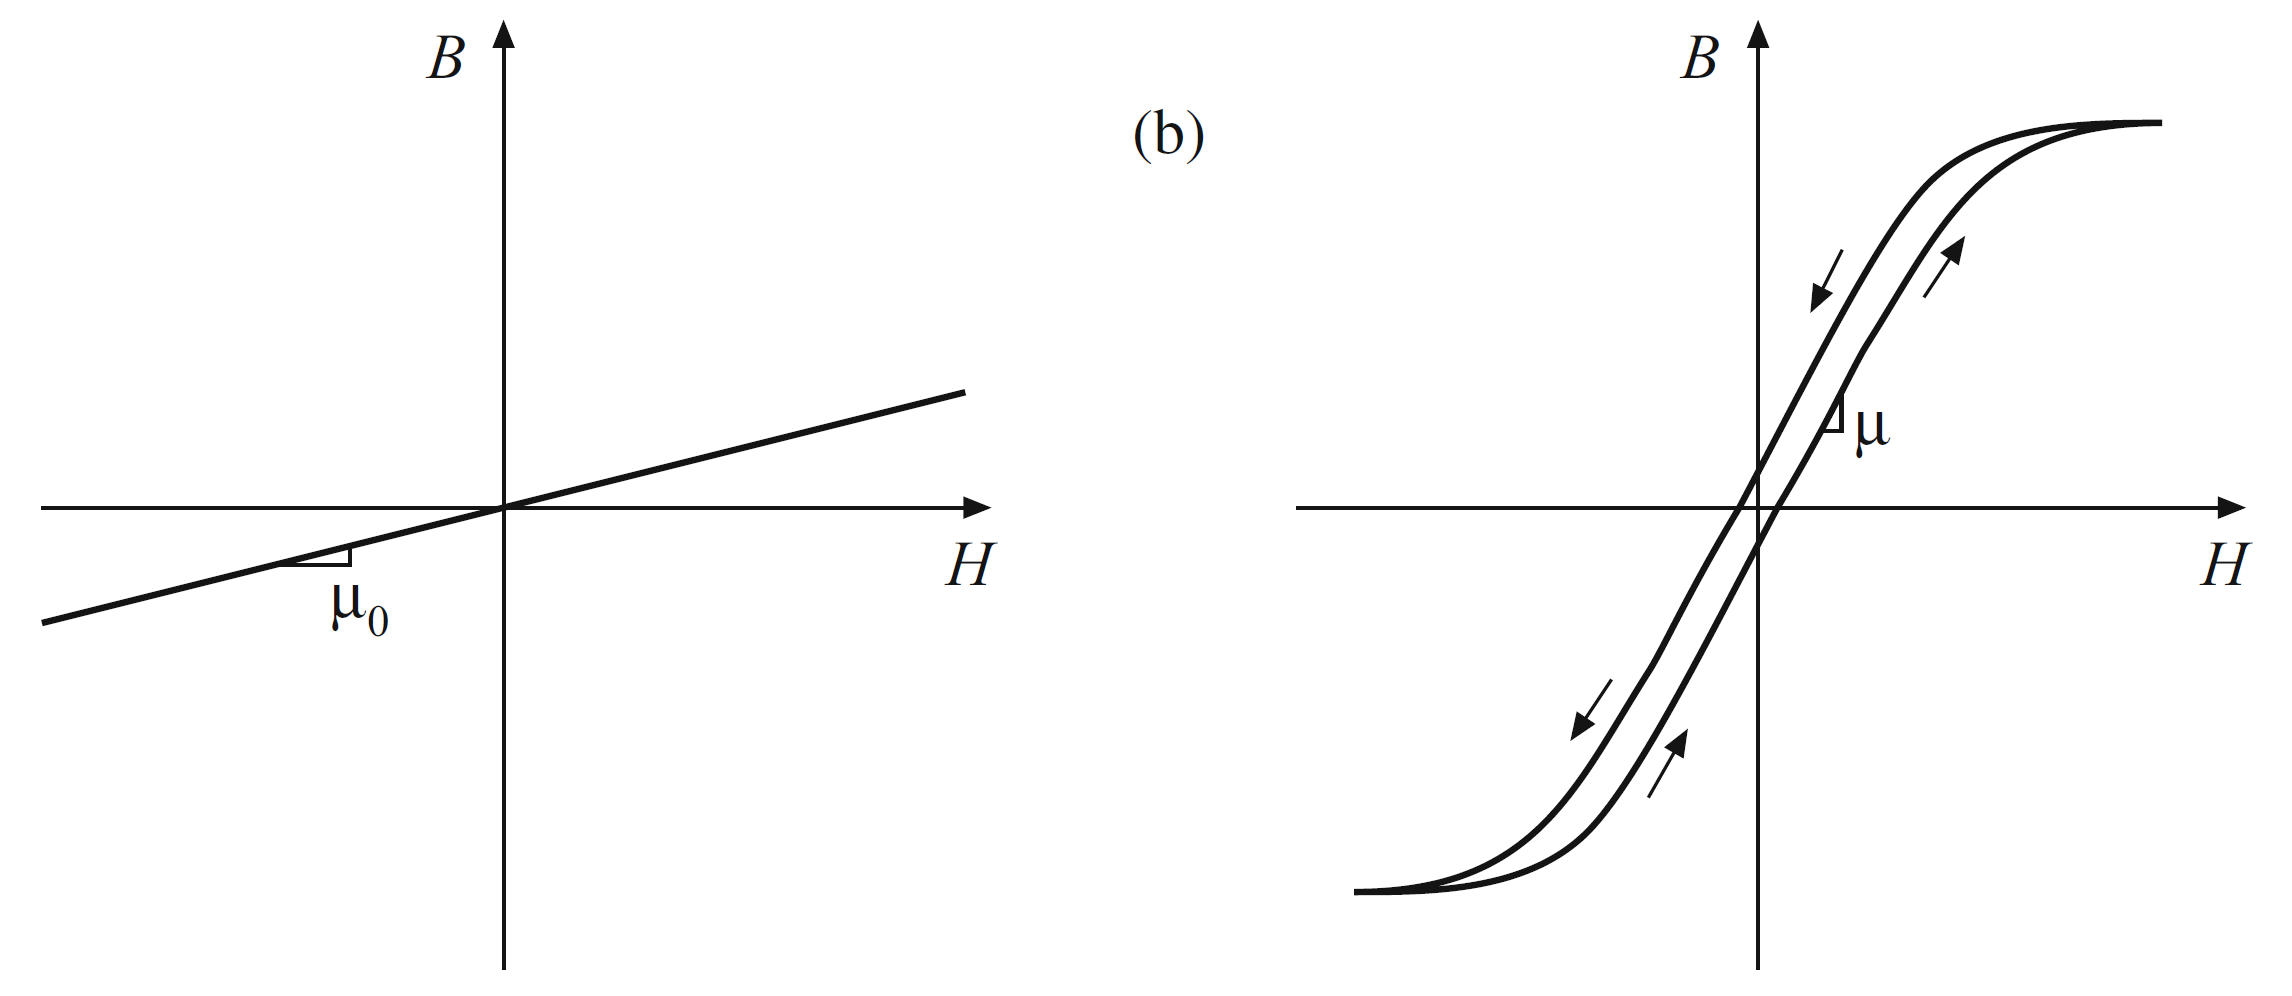
\includegraphics[width=\linewidth]{fig/lec07/air_core_material.png} 
                \caption{$B$--$H$ characteristics of air and a typical magnetic core material. Adapted from Erickson and Maksimovi\'c, Fig. 10.5.} 
            \end{figure} 
            A high value of $\mu$ means that a relatively small $H$ can produce a large $B$. 
        \end{column} 
    \end{columns} 
\end{frame}


%%%%%%%%%%%%%%%%%%%%%%%%%%%%%%%%%%%%%%%%%%%%%%%%%%%%%%%%%%%%% %% Ideal B-H curve %%%%%%%%%%%%%%%%%%%%%%%%%%%%%%%%%%%%%%%%%%%%%%%%%%%%%%%%%%%%%
\begin{frame} 
    \frametitle{Idealized $B$--$H$ Characteristic} 
    \begin{columns} 
        \begin{column}{0.57\textwidth} 
            For introductory analysis, a magnetic material is often represented using an idealized or piecewise-linear $B$--$H$ characteristic. 
            \begin{align} 
                B=\mu H 
            \end{align} 
            In the linear region, 
            \begin{itemize} 
                \item the slope of the $B$--$H$ curve is the permeability $\mu$, 
                \item flux density increases almost linearly with field intensity, 
                \item the core behaves as a predictable magnetic path, 
                \item inductance remains approximately constant. 
            \end{itemize} 
            \vspace{0.15cm} 
            However, this linear model is only valid before saturation. At high excitation, the material cannot support proportional increase in flux density. 
            \begin{align} 
                B \rightarrow B_{\mathrm{sat}} 
            \end{align} 
        \end{column} 
        \begin{column}{0.39\textwidth} 
            \begin{figure} 
                \centering 
                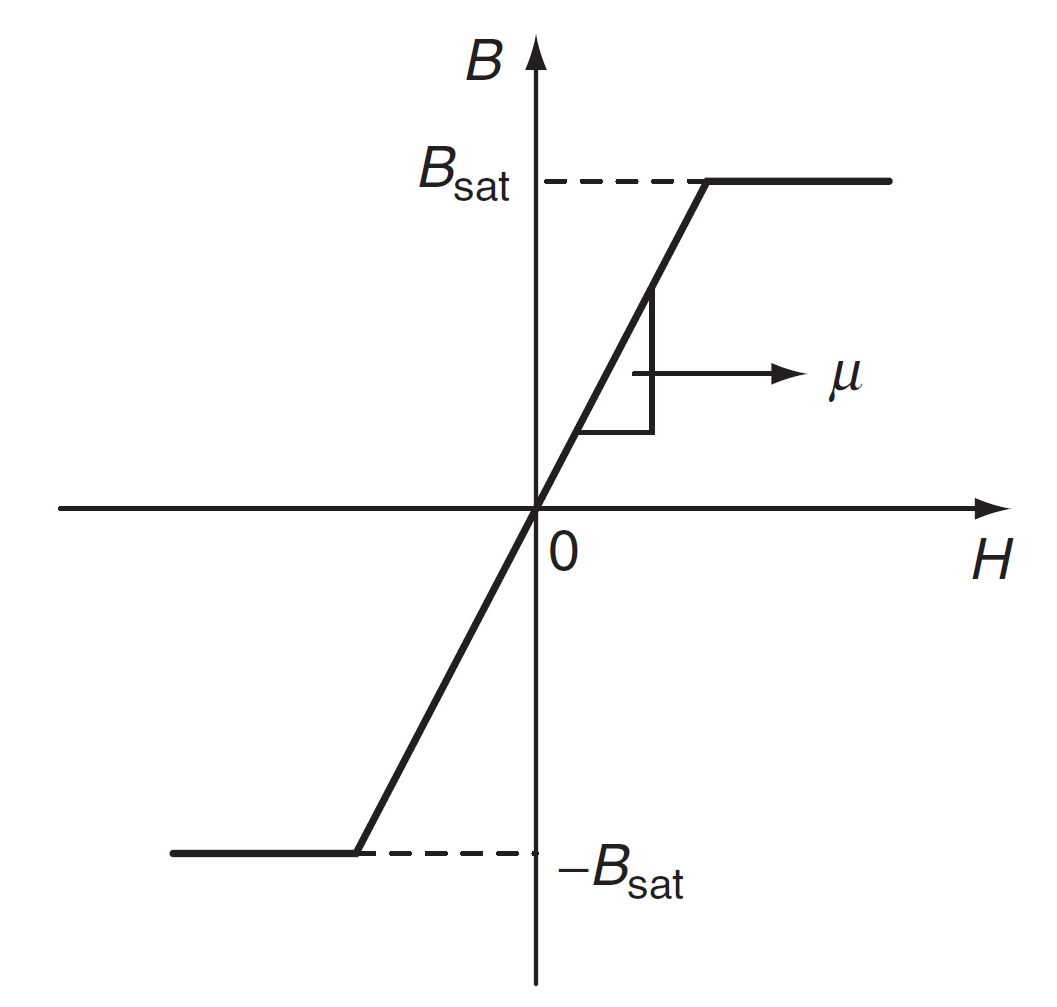
\includegraphics[width=0.8\linewidth]{fig/lec07/piecewise_linear_BH.png} 
                \caption{Piecewise-linear approximation of the $B$--$H$ curve. Adapted from Umanand, \textit{Power Electronics: Essentials and Applications}, 2nd edition, Wiley, 2012.}
            \end{figure} 
        \end{column} 
    \end{columns} 
\end{frame}


%%%%%%%%%%%%%%%%%%%%%%%%%%%%%%%%%%%%%%%%%%%%%%%%%%%%%%%%%%%%% %% Practical B-H curve and hysteresis %%%%%%%%%%%%%%%%%%%%%%%%%%%%%%%%%%%%%%%%%%%%%%%%%%%%%%%%%%%%%
\begin{frame} 
    \frametitle{Practical $B$--$H$ Characteristic and Hysteresis}
    \begin{columns} 
        \begin{column}{0.57\textwidth} 
            Practical magnetic materials do not follow a single-valued linear $B$--$H$ curve. Instead, they exhibit hysteresis: the flux density depends not only on the present value of $H$, but also on the previous magnetic history. 
            \vspace{0.15cm} 
            \begin{itemize} 
                \item During magnetization, energy is stored in the magnetic field. 
                \item During demagnetization, not all stored energy is returned. 
                \item The enclosed area of the $B$--$H$ loop represents energy lost per cycle. 
                \item This loss appears as heat in the magnetic core. 
                \item Hysteresis loss increases with switching frequency. 
            \end{itemize} 
        \end{column} 
        \begin{column}{0.39\textwidth} 
            \vspace{-0.5cm}
            \begin{figure} 
                \centering 
                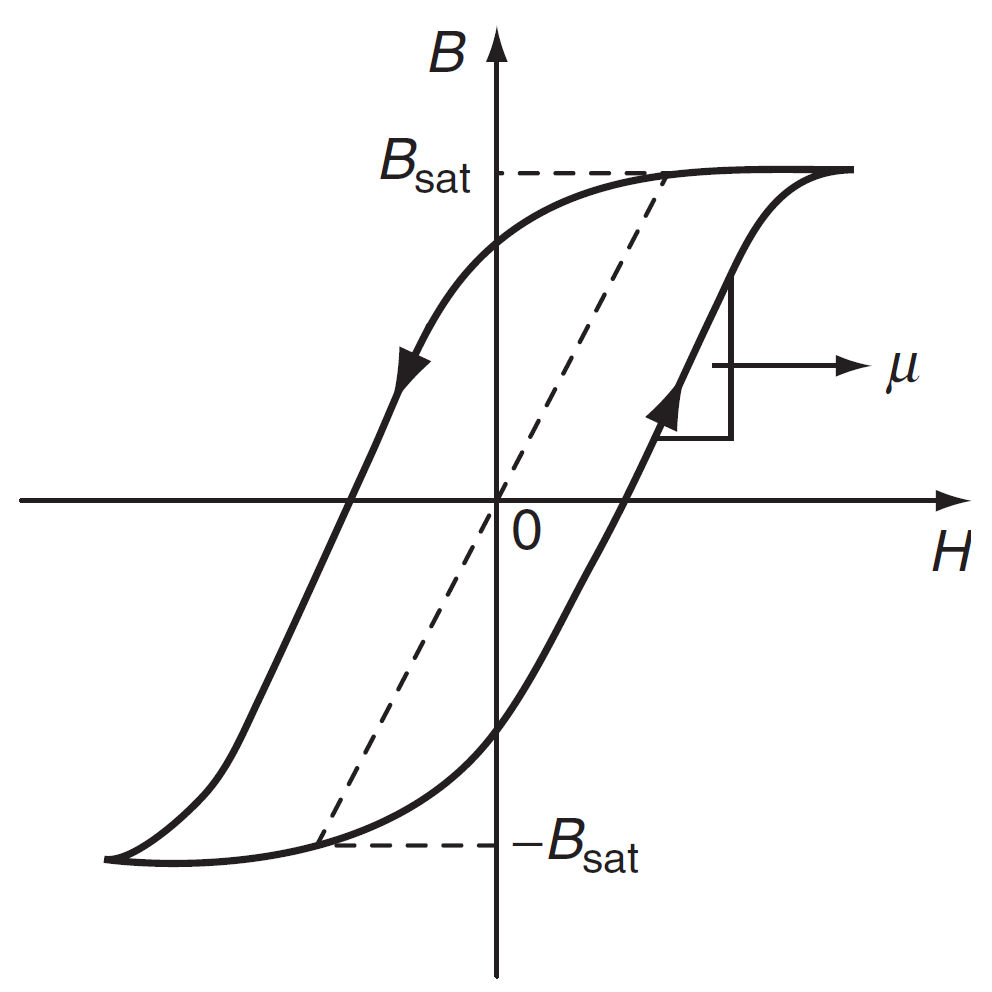
\includegraphics[width=0.7\linewidth]{fig/lec07/practical_BH_loop.png} 
                \caption{Practical $B$--$H$ loop showing hysteresis. Adapted from Umanand, \textit{Power Electronics: Essentials and Applications}, 2nd edition, Wiley, 2012.}
            \end{figure} 
            The core-loss energy density per cycle is proportional to 
            \begin{align} 
                W_{\mathrm{hyst}} \propto \oint H\,dB 
            \end{align} 
        \end{column} 
    \end{columns} 
\end{frame}


%%%%%%%%%%%%%%%%%%%%%%%%%%%%%%%%%%%%%%%%%%%%%%%%%%%%%%%%%%%%% %% Saturation flux density %%%%%%%%%%%%%%%%%%%%%%%%%%%%%%%%%%%%%%%%%%%%%%%%%%%%%%%%%%%%%
\begin{frame} 
    \frametitle{Saturation Flux Density of Magnetic Materials} 
    \begin{columns} 
        \begin{column}{0.56\textwidth} 
            The saturation flux density $B_{\mathrm{sat}}$ is a key material limit. If the operating flux density approaches this value, the effective permeability collapses and the magnetic component can no longer behave as intended. 
            \vspace{0.15cm} 
            \begin{table} 
                \centering 
                \small 
                \begin{tabular}{lc} 
                    \hline 
                    \textbf{Core material} & \textbf{Typical $B_{\mathrm{sat}}$}\\ 
                    \hline 
                    Ferrite & $\approx 0.3\ \si{\tesla}$\\
                    Silicon steel & $\approx 1.0$--$1.2\ \si{\tesla}$\\ 
                    Powdered iron & $\approx 1.6\ \si{\tesla}$\\ 
                    Amorphous core & $\approx 1.6\ \si{\tesla}$\\ 
                    Mu-metal & $\approx 1.0\ \si{\tesla}$\\ \hline 
                \end{tabular} 
            \end{table} 
            \vspace{0.1cm} 
            These values provide first-order design limits. Practical operation usually uses lower peak flux density to limit core loss and temperature rise. 
        \end{column} 
        \begin{column}{0.40\textwidth} 
            \begin{block}{Power Electronics Interpretation} 
                \small High $B_{\mathrm{sat}}$ enables smaller cores, but high-frequency operation is often limited more strongly by core loss than by saturation. Ferrites have lower $B_{\mathrm{sat}}$, but are widely used at high frequency because of their relatively low eddy-current loss. 
            \end{block} 
         \end{column} 
    \end{columns} 
\end{frame}

%%%%%%%%%%%%%%%%%%%%%%%%%%%%%%%%%%%%%%%%%%%%%%%%%%%%%%%%%%%%% %% Reluctance %%%%%%%%%%%%%%%%%%%%%%%%%%%%%%%%%%%%%%%%%%%%%%%%%%%%%%%%%%%%%
\begin{frame} 
    \frametitle{Reluctance: Opposition to Magnetic Flux} 
    \begin{columns} 
        \begin{column}{0.58\textwidth} 
            In an electrical circuit, resistance opposes current flow. Similarly, in a magnetic circuit, reluctance opposes magnetic flux. 
            Starting from 
                $H=\frac{Ni}{l_m}$ and $B=\mu H$ 
            with $\Phi=BA_c$, one obtains 
            \begin{align} 
                \Phi = \frac{Ni\,\mu A_c}{l_m} 
            \end{align} or 
            \begin{align} 
                \Phi = \frac{F}{\mathcal R} 
            \end{align} 
            where $\mathcal R = \frac{l_m}{\mu A_c}$ is called the magnetic reluctance.
            \begin{itemize}
                \item Long magnetic paths increase reluctance. 
                \item Large core area reduces reluctance. 
                \item High permeability reduces reluctance. 
            \end{itemize} 
        \end{column} 
        \begin{column}{0.38\textwidth} 
            \begin{block}{Electrical Analogy} 
                \begin{align} 
                    I=\frac{V}{R} 
                \end{align} 
                \begin{align} 
                    \Phi=\frac{F}{\mathcal R} 
                \end{align} 
            \end{block} 
            \begin{itemize} 
                \item Voltage $\leftrightarrow$ MMF 
                \item Current $\leftrightarrow$ Flux 
                \item Resistance $\leftrightarrow$ Reluctance 
            \end{itemize} 
        \end{column} 
    \end{columns} 
\end{frame}


%%%%%%%%%%%%%%%%%%%%%%%%%%%%%%%%%%%%%%%%%%%%%%%%%%%%%%%%%%%%% %% Permeance %%%%%%%%%%%%%%%%%%%%%%%%%%%%%%%%%%%%%%%%%%%%%%%%%%%%%%%%%%%%%
\begin{frame} 
    \frametitle{Permeance: Ease of Magnetic Flux Flow} 
    \begin{columns} 
        \begin{column}{0.58\textwidth} 
            The reciprocal of reluctance is called permeance. 
            \begin{align} 
                \Lambda = \frac{1}{\mathcal R} 
            \end{align} 
            Substituting the reluctance expression gives 
                $\Lambda = \frac{\mu A_c}{l_m}$ 
            Therefore $
                \Phi=\Lambda F $
                Permeance describes how easily magnetic flux can be established within a magnetic path. 
                \begin{itemize} 
                    \item Large cross-sectional area increases permeance. 
                    \item High permeability materials increase permeance. 
                    \item Longer magnetic paths decrease permeance. 
                \end{itemize} 
            \end{column} 
            \begin{column}{0.38\textwidth} 
                \begin{block}{Electrical Analogy} 
                    Conductance: 
                    \begin{align} 
                        G=\frac{1}{R} 
                    \end{align} 
                    Magnetic equivalent: 
                    \begin{align} 
                        \Lambda=\frac{1}{\mathcal R} 
                    \end{align} 
                \end{block} 
                Permeance plays a role analogous to capacitance in the magnetic energy-storage viewpoint discussed. 
        \end{column} 
    \end{columns} 
\end{frame}

%%%%%%%%%%%%%%%%%%%%%%%%%%%%%%%%%%%%%%%%%%%%%%%%%%%%%%%%%%%%% %% Magnetic circuits %%%%%%%%%%%%%%%%%%%%%%%%%%%%%%%%%%%%%%%%%%%%%%%%%%%%%%%%%%%%% 
\begin{frame} 
    \frametitle{Magnetic Circuit Representation} 
    \begin{columns} 
        \begin{column}{0.58\textwidth} 
            Magnetic components are often represented using equivalent magnetic circuits. 
            \vspace{0.15cm} 
            The governing magnetic-circuit equation is 
            \begin{align} 
                F=\Phi\mathcal R 
            \end{align} 
            \vspace{0.15cm} 
            Using this representation: 
            \begin{itemize} 
                \item Flux can be calculated using circuit techniques. 
                \item Air gaps can be incorporated naturally. 
                \item Core saturation can be interpreted physically. 
                \item Inductance calculations become straightforward. 
            \end{itemize} 
        \end{column} 
        \begin{column}{0.38\textwidth} 
            \begin{figure} 
                \centering 
                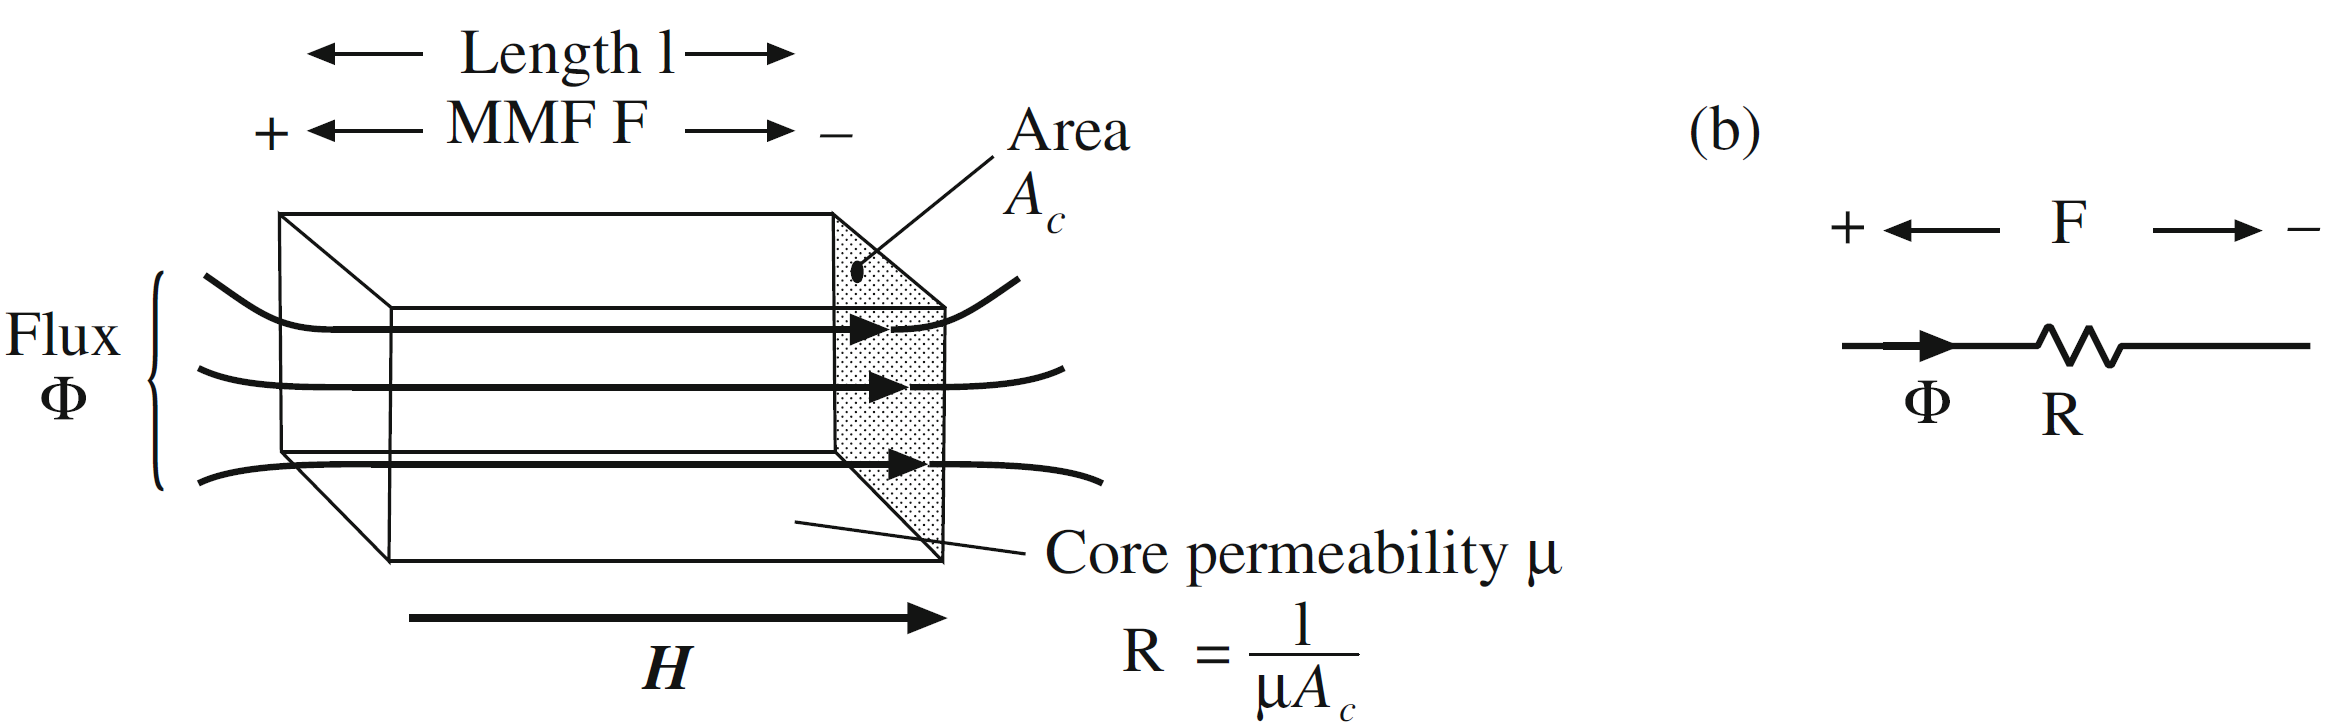
\includegraphics[width=\linewidth]{fig/lec07/magnetic_circuit_equivalent.png} 
                \caption{Equivalent magnetic circuit representation of a magnetic core. Adapted from Erickson and Maksimovi\'c, \textit{Fundamentals of Power Electronics}, 3rd edition, Springer, 2013.}
            \end{figure} 
        \end{column} 
    \end{columns} 
\end{frame}

%%%%%%%%%%%%%%%%%%%%%%%%%%%%%%%%%%%%%%%%%%%%%%%%%%%%%%%%%%%%% %% Series magnetic circuit %%%%%%%%%%%%%%%%%%%%%%%%%%%%%%%%%%%%%%%%%%%%%%%%%%%%%%%%%%%%%
\begin{frame} 
    \frametitle{Series Magnetic Circuits} 
    \begin{columns} 
        \begin{column}{0.58\textwidth} 
            When magnetic flux passes sequentially through several sections of a magnetic path, the corresponding reluctances are connected in series. 
            \begin{align} 
                \mathcal R_{eq} = \mathcal R_1 + \mathcal R_2 + \mathcal R_3 +\cdots 
            \end{align} 
            The same magnetic flux flows through all sections: 
            \begin{align} 
                \Phi_1=\Phi_2=\Phi_3 
            \end{align} 
            The total MMF is 
            \begin{align} 
                F=\Phi \mathcal R_{eq} 
            \end{align} 
            \vspace{0.15cm}  
        \end{column} 
        \begin{column}{0.38\textwidth} 
            \begin{block}{Electrical Equivalent} 
                \begin{align} 
                    R_{eq}=R_1+R_2+R_3 
                \end{align} 
            \end{block} 
            \vspace{0.2cm} 
            Exactly the same mathematical rules apply to reluctances. Examples: 
            \begin{itemize} 
                \item Core section + air gap. 
                \item Multi-material magnetic path. 
                \item Practical transformer cores. 
            \end{itemize}
        \end{column} 
    \end{columns} 
\end{frame}


%%%%%%%%%%%%%%%%%%%%%%%%%%%%%%%%%%%%%%%%%%%%%%%%%%%%%%%%%%%%% %% Air gap reluctance %%%%%%%%%%%%%%%%%%%%%%%%%%%%%%%%%%%%%%%%%%%%%%%%%%%%%%%%%%%%%
\begin{frame} 
    \frametitle{Why Does the Air Gap Dominate Reluctance?} 
    \begin{columns} 
        \begin{column}{0.58\textwidth} 
            Consider a magnetic core containing a small air gap $l_g$. The total reluctance becomes 
            \begin{align} 
                \mathcal R = \frac{l_m}{\mu_0\mu_r A_c} + \frac{l_g}{\mu_0A_c} 
            \end{align} 
            Since 
                $\mu_r \gg 1$ 
            for practical magnetic materials, 
            \begin{align} 
                \mathcal R \approx \frac{l_g}{\mu_0A_c} 
            \end{align} 
            \vspace{0.15cm} 
            Therefore: 
            \begin{itemize} 
                \item Even a very small air gap dominates the total reluctance. 
                \item The effective permeability decreases dramatically. 
                \item Saturation current increases significantly. 
            \end{itemize} 
        \end{column} 
        \begin{column}{0.38\textwidth} 
            \begin{figure} 
                \centering 
                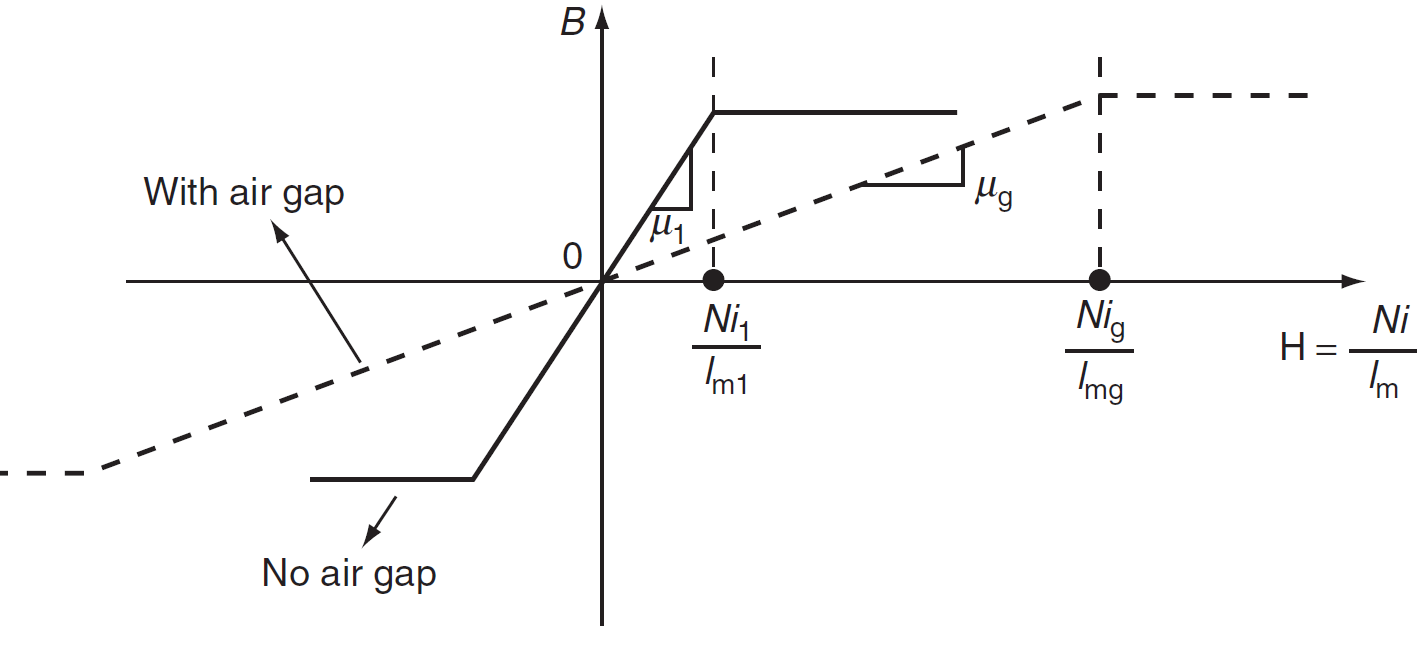
\includegraphics[width=\linewidth]{fig/lec07/air_gap_effect.png} 
                \caption{Effect of air-gap introduction on magnetic characteristics. Adapted from Umanand, \textit{Power Electronics: Essentials and Applications}, 2nd edition, Wiley, 2012.}
            \end{figure} 
        \end{column} 
    \end{columns} 
\end{frame}

%%%%%%%%%%%%%%%%%%%%%%%%%%%%%%%%%%%%%%%%%%%%%%%%%%%%%%%%%%%%% %% Flux division %%%%%%%%%%%%%%%%%%%%%%%%%%%%%%%%%%%%%%%%%%%%%%%%%%%%%%%%%%%%% 
\begin{frame} 
    \frametitle{Parallel Magnetic Circuits and Flux Division} 
    \begin{columns} 
        \begin{column}{0.58\textwidth} 
            Just as electric current divides among parallel resistors, magnetic flux divides among parallel reluctance paths. 
            \vspace{0.15cm} 
            For two parallel paths, 
            \begin{align} 
                \Phi = \Phi_1+\Phi_2 \quad F_1=F_2 
            \end{align}
            The flux distribution becomes 
            \begin{align} 
                \Phi_1 = \frac{F}{\mathcal R_1} 
            \end{align} 
            \begin{align} 
                \Phi_2 = \frac{F}{\mathcal R_2} 
            \end{align} 
            Flux naturally prefers the lower-reluctance path. 
        \end{column} 
        \begin{column}{0.38\textwidth} 
            \begin{block}{Important Observation} 
                High-permeability materials attract magnetic flux. 
                This principle explains: 
                \begin{itemize} 
                    \item Magnetic shielding 
                    \item Flux concentrators 
                    \item Core shaping 
                    \item Leakage-flux paths 
                \end{itemize} 
            \end{block} 
        \end{column} 
    \end{columns} 
\end{frame}


%%%%%%%%%%%%%%%%%%%%%%%%%%%%%%%%%%%%%%%%%%%%%%%%%%%%%%%%%%%%% %% Volt second balance %%%%%%%%%%%%%%%%%%%%%%%%%%%%%%%%%%%%%%%%%%%%%%%%%%%%%%%%%%%%% 
\begin{frame} 
    \frametitle{Volt-Second Balance: Fundamental Principle} 
    \begin{columns} 
        \begin{column}{0.58\textwidth} 
            Starting from Faraday's law, 
            \begin{align} 
                v=N A_c\frac{dB}{dt} 
            \end{align} 
            Integrating over one switching period, 
            \begin{align} 
                \int_0^T v(t)dt = NA_c \int_0^T dB 
            \end{align} 
            For periodic steady-state operation, 
            \begin{align} 
                B(T)=B(0) 
            \end{align} 
            Therefore, is the volt-second balance condition: 
            \begin{align} 
                \int_0^T v(t)dt=0 
            \end{align} 
        \end{column} 
        \begin{column}{0.38\textwidth} 
            \begin{block}{Physical Meaning} The average voltage across a magnetic winding must be zero in steady state. Otherwise flux continues to accumulate cycle after cycle. 
            \end{block} 
        \end{column} 
    \end{columns} 
\end{frame}

%%%%%%%%%%%%%%%%%%%%%%%%%%%%%%%%%%%%%%%%%%%%%%%%%%%%%%%%%%%%% %% Volt second and saturation %%%%%%%%%%%%%%%%%%%%%%%%%%%%%%%%%%%%%%%%%%%%%%%%%%%%%%%%%%%%% 
\begin{frame} 
    \frametitle{Flux Build-Up and Core Saturation} 
    \begin{columns} 
        \begin{column}{0.58\textwidth} 
            From \begin{align} B = \frac{1}{NA_c} \int v(t)dt 
            \end{align} 
            we observe that flux density is determined by the accumulated volt-seconds. 
            \vspace{0.15cm} 
            If 
            \begin{align} 
                \frac{1}{T} \int_0^T v(t)dt \neq 0 
            \end{align} 
            then $B \rightarrow \infty$ in the ideal mathematical model. Practically, the flux density reaches 
            \begin{align} 
                B_{sat} 
            \end{align} 
            and the core saturates. 
        \end{column} 
        \begin{column}{0.38\textwidth} 
            \begin{block}{Design Implication} 
                A transformer can saturate even at low load current if volt-second balance is violated. 
                \vspace{0.15cm} 
                Transformer saturation is governed primarily by flux density, not by output current. 
            \end{block} 
        \end{column} 
    \end{columns} 
\end{frame}

%%%%%%%%%%%%%%%%%%%%%%%%%%%%%%%%%%%%%%%%%%%%%%%%%%%%%%%%%%%%% %% Volt second example %%%%%%%%%%%%%%%%%%%%%%%%%%%%%%%%%%%%%%%%%%%%%%%%%%%%%%%%%%%%% 
\begin{frame} 
    \frametitle{Example: Volt-Second Balance in a Square-Wave Excitation} 
    \begin{columns} 
        \begin{column}{0.58\textwidth} 
            Consider a winding excited by 
            \begin{align} +V \quad \mathrm{for}\quad \frac{T}{2} \quad \text{and} \quad -V \quad \mathrm{for}\quad \frac{T}{2} 
            \end{align} 
            The total volt-seconds become 
            \begin{align} 
                VT/2 - VT/2 =0 
            \end{align} 
            Hence, 
            \begin{itemize} 
                \item Flux oscillates around zero. 
                \item No long-term flux accumulation occurs. 
                \item Core saturation is avoided. 
            \end{itemize} 
            This is the operating principle of ideal transformer excitation. 
        \end{column} 
        \begin{column}{0.38\textwidth} 
            \begin{figure} 
                \centering 
                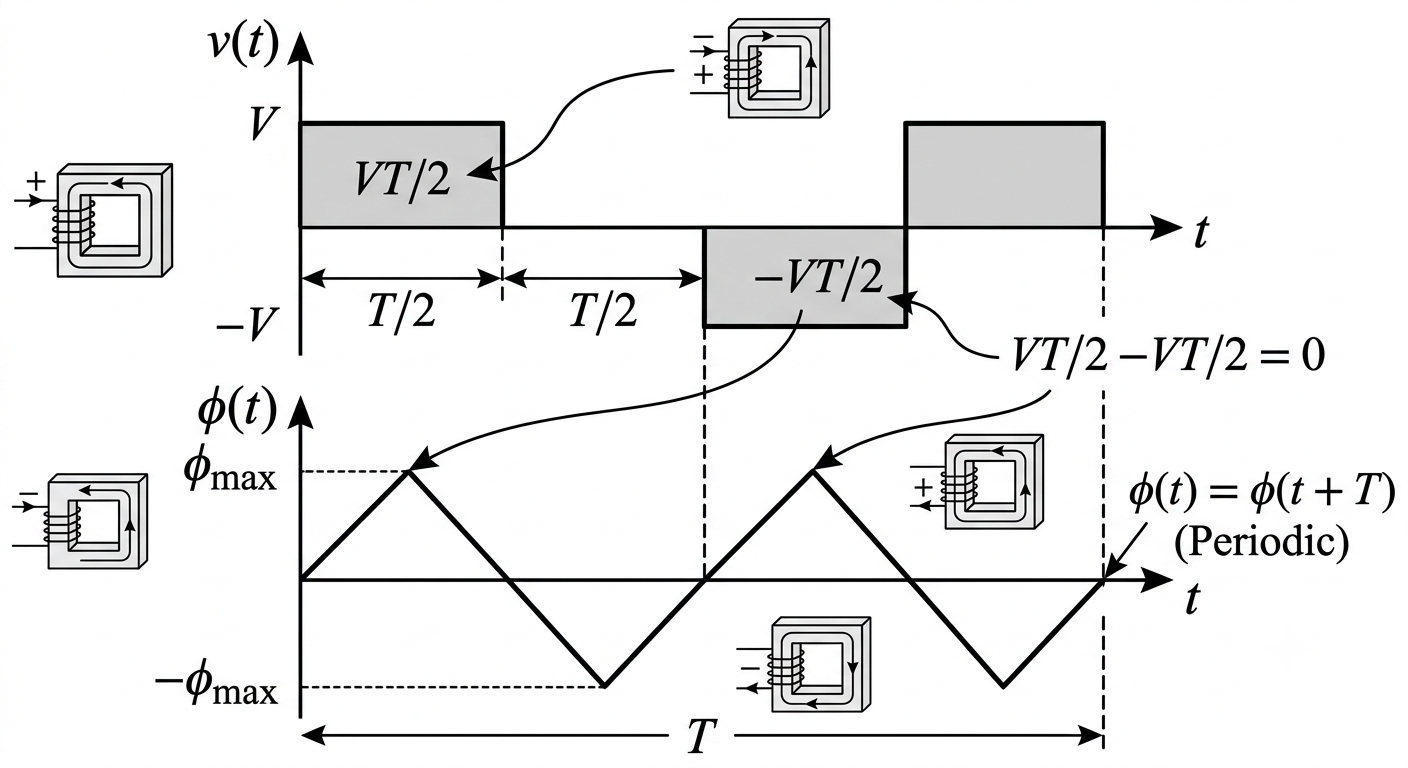
\includegraphics[width=\linewidth]{fig/lec07/square_wave_volt_second_balance.png} 
                \caption{Balanced positive and negative volt-seconds leading to periodic flux excursion.} 
            \end{figure} 
        \end{column} 
    \end{columns} 
\end{frame}

% %%%%%%%%%%%%%%%%%%%%%%%%%%%%%%%%%%%%%%%%%%%%%%%%%%%%%%%%%%%%% %% Inductor concept %%%%%%%%%%%%%%%%%%%%%%%%%%%%%%%%%%%%%%%%%%%%%%%%%%%%%%%%%%%%%
% \begin{frame} 
%     \frametitle{What is an Inductor?} 
%     \begin{columns} 
%         \begin{column}{0.58\textwidth} 
%             An inductor is a magnetic component that stores energy in its magnetic field when current flows through its winding. 
%             \vspace{0.15cm} Unlike transformers, which ideally transfer energy from one winding to another, inductors are specifically designed to store energy temporarily. 
%             \vspace{0.15cm} 
%             Typical applications include: 
%             \begin{itemize} 
%                 \item Buck converters 
%                 \item Boost converters 
%                 \item Flyback converters 
%                 \item EMI filters 
%                 \item Resonant converters 
%                 \item Motor drives 
%             \end{itemize} 
%             \vspace{0.15cm} 
%         \end{column} 
%         \begin{column}{0.38\textwidth} 
%             The electrical behaviour of an inductor is governed by 
%             \begin{align} 
%                 v=L\frac{di}{dt} 
%             \end{align} 
%             which indicates that an inductor opposes changes in current. 
%             \begin{block}{Physical Interpretation} 
%                 Current establishes magnetic flux. 
%                 \vspace{0.1cm} 
%                 The magnetic field stores energy and resists abrupt changes in current. 
%             \end{block} 
%         \end{column} 
%     \end{columns} 
% \end{frame}


% %%%%%%%%%%%%%%%%%%%%%%%%%%%%%%%%%%%%%%%%%%%%%%%%%%%%%%%%%%%%% %% Inductor derivation %%%%%%%%%%%%%%%%%%%%%%%%%%%%%%%%%%%%%%%%%%%%%%%%%%%%%%%%%%%%%
% \begin{frame} 
%     \frametitle{Derivation of Inductance from Magnetic Circuits} 
%     \begin{columns} 
%         \begin{column}{0.58\textwidth} 
%             Starting from the magnetic circuit relation 
%                 $\Phi=\Lambda Ni$.
%             Differentiating with respect to time, 
%             \begin{align} 
%                 \frac{d\Phi}{dt} = \Lambda N \frac{di}{dt} 
%             \end{align} 
%             Applying Faraday's law, 
%             \begin{align} 
%                 v = N\frac{d\Phi}{dt} \text{yields} \quad v = \Lambda N^2 \frac{di}{dt}
%             \end{align} 
%             Comparing with 
%             \begin{align} 
%                 v=L\frac{di}{dt} \quad \Longrightarrow \quad L=\Lambda N^2
%             \end{align} 
%         \end{column} 
%         \begin{column}{0.38\textwidth} 
%             \begin{block}{Important Result} 
%                 \begin{align} 
%                     L=\Lambda N^2 
%                 \end{align} 
%                 \vspace{0.1cm} 
%                 Inductance is determined by \begin{itemize} \item Number of turns \item Core geometry \item Core permeability \item Air gap \end{itemize} 
%             \end{block} 
%         \end{column} 
%     \end{columns} 
% \end{frame}

%%%%%%%%%%%%%%%%%%%%%%%%%%%%%%%%%%%%%%%%%%%%%%%%%%%%%%%%%%%%% %% Physical inductance %%%%%%%%%%%%%%%%%%%%%%%%%%%%%%%%%%%%%%%%%%%%%%%%%%%%%%%%%%%%% 
\begin{frame} 
    \frametitle{Physical Expression for Inductance} 
    \begin{columns} 
        \begin{column}{0.58\textwidth} 
            Substituting 
                $\Lambda=\frac{\mu A_c}{l_m}$ 
            into $
                L=\Lambda N^2 $
            gives 
            \begin{align} 
                L= \frac{\mu A_c N^2}{l_m} 
            \end{align} 
            This expression reveals the physical parameters that determine inductance. 
            \vspace{0.15cm} 
            \begin{itemize} 
                \item Increasing turns increases inductance quadratically. 
                \item Increasing permeability increases inductance. 
                \item Increasing core area increases inductance. 
                \item Increasing magnetic path length reduces inductance. 
            \end{itemize} 
        \end{column} 
        \begin{column}{0.38\textwidth} 
            \begin{block}{Design Insight} 
                \begin{align} 
                    L \propto N^2 
                \end{align} 
                Doubling the number of turns increases inductance by a factor of four. 
            \end{block} 
        \end{column} 
    \end{columns} 
\end{frame}


%%%%%%%%%%%%%%%%%%%%%%%%%%%%%%%%%%%%%%%%%%%%%%%%%%%%%%%%%%%%% %% Energy storage %%%%%%%%%%%%%%%%%%%%%%%%%%%%%%%%%%%%%%%%%%%%%%%%%%%%%%%%%%%%% 
\begin{frame} 
    \frametitle{Energy Stored in an Inductor} 
    \begin{columns} 
        \begin{column}{0.58\textwidth} 
            The energy stored in an inductor is 
            \begin{align} 
                E_L = \int vi\,dt 
            \end{align} 
            Substituting 
                $v=L\frac{di}{dt}$ 
            gives 
            \begin{align} 
                E_L = \int Li\,di 
            \end{align} 
            which yields 
            \begin{align} 
                E_L = \frac12 LI^2 
            \end{align} 
            \vspace{0.15cm} 


        \end{column} 
        \begin{column}{0.38\textwidth}
            Key observations:  
            \begin{itemize} 
                \item Energy increases with current squared. 
                \item Energy is recoverable. 
                \item Inductors are energy-storage devices. 
                \item Larger currents require significantly larger stored energy capability. 
            \end{itemize} 
            \begin{block}{Example} 
                If $L=100\ \mu H $ and $I=10A$ then $E_L=5\,mJ$ 
            \end{block} 
        \end{column} 
    \end{columns} 
\end{frame}


%%%%%%%%%%%%%%%%%%%%%%%%%%%%%%%%%%%%%%%%%%%%%%%%%%%%%%%%%%%%% %% Energy storage physical meaning %%%%%%%%%%%%%%%%%%%%%%%%%%%%%%%%%%%%%%%%%%%%%%%%%%%%%%%%%%%%% 
\begin{frame} 
    \frametitle{Where is the Energy Actually Stored?} 
    \begin{columns} 
        \begin{column}{0.58\textwidth} 
            A common misconception is that energy is stored in the magnetic core. 
            \vspace{0.15cm} 
            In reality, energy is stored in the magnetic field itself. 
            \vspace{0.15cm} 
            The magnetic energy density is 
            \begin{align} 
                w_m = \frac12 BH 
            \end{align} 
            and total stored energy becomes 
            \begin{align} 
                E=\int_V \frac12 BH\,dV 
            \end{align} 
            \vspace{0.15cm} 
            For gapped inductors: 
            \begin{itemize} 
                \item Most stored energy resides in the air gap. 
                \item The magnetic core primarily guides flux. 
                \item The air gap acts as the main energy-storage region. 
            \end{itemize} 
        \end{column} 
        \begin{column}{0.38\textwidth} 
            \begin{block}{Important Concept} 
                Transformer \[ \text{Transfer energy} \] 
                Inductor \[ \text{Store energy} \] 
                This distinction drives completely different magnetic designs. 
            \end{block} 
        \end{column} 
    \end{columns} 
\end{frame}



\begin{frame}{Magnetic Materials Used in Power Electronics}
Magnetic materials are selected according to the operating frequency, allowable flux density, core loss and cost. No single material is optimal for all applications.
\begin{table}
\centering
\footnotesize
\begin{tabular}{lccc}
\toprule
Material & Typical $B_{\mathrm{sat}}$ & Frequency Range & Typical Applications\\
\midrule
Silicon steel & 1.0--2.0 T & 50--400 Hz & Grid transformers\\
Ferrite & 0.25--0.5 T & 20 kHz--2 MHz & SMPS, LLC, Flyback\\
Powdered iron & 0.6--1.6 T & up to $\sim$500 kHz & PFC inductors\\
Amorphous alloy & 0.8--1.5 T & kHz range & High-efficiency transformers\\
Nanocrystalline & 1.1--1.3 T & up to MHz & EV, aerospace magnetics\\
\bottomrule
\end{tabular}
\end{table}

\begin{block}{Design Insight}
High-frequency converters generally favour ferrite cores because their extremely high electrical resistivity suppresses eddy-current loss, even though their saturation flux density is relatively low. Conversely, silicon-steel cores offer much higher saturation flux density but become unsuitable
for high-frequency operation due to excessive core loss.
\end{block}
\end{frame}

\begin{frame}{Core Loss versus Frequency}
    \begin{columns} 
        \begin{column}{0.58\textwidth}
Core loss increases rapidly with switching frequency.
Two physical mechanisms contribute:

\begin{itemize}
\item \textbf{Hysteresis loss} caused by repeated reversal of magnetic domains.
\item \textbf{Eddy-current loss} caused by induced circulating currents inside the core.
\end{itemize}

The total core loss is commonly approximated using the Steinmetz equation
\[
P_{\mathrm{core}}
=
k
f^{\alpha}
B_{\mathrm{pk}}^{\beta}
V_{\mathrm{core}}
\]
\begin{itemize}
\item $f$ is switching frequency,
\item $B_{\mathrm{pk}}$ is peak flux density,
\item $V_{\mathrm{core}}$ is core volume,
\item $k,\alpha,\beta$ are material-dependent constants.
\end{itemize}
\end{column} 

\begin{column}{0.38\textwidth}
            \begin{figure} 
                \centering 
                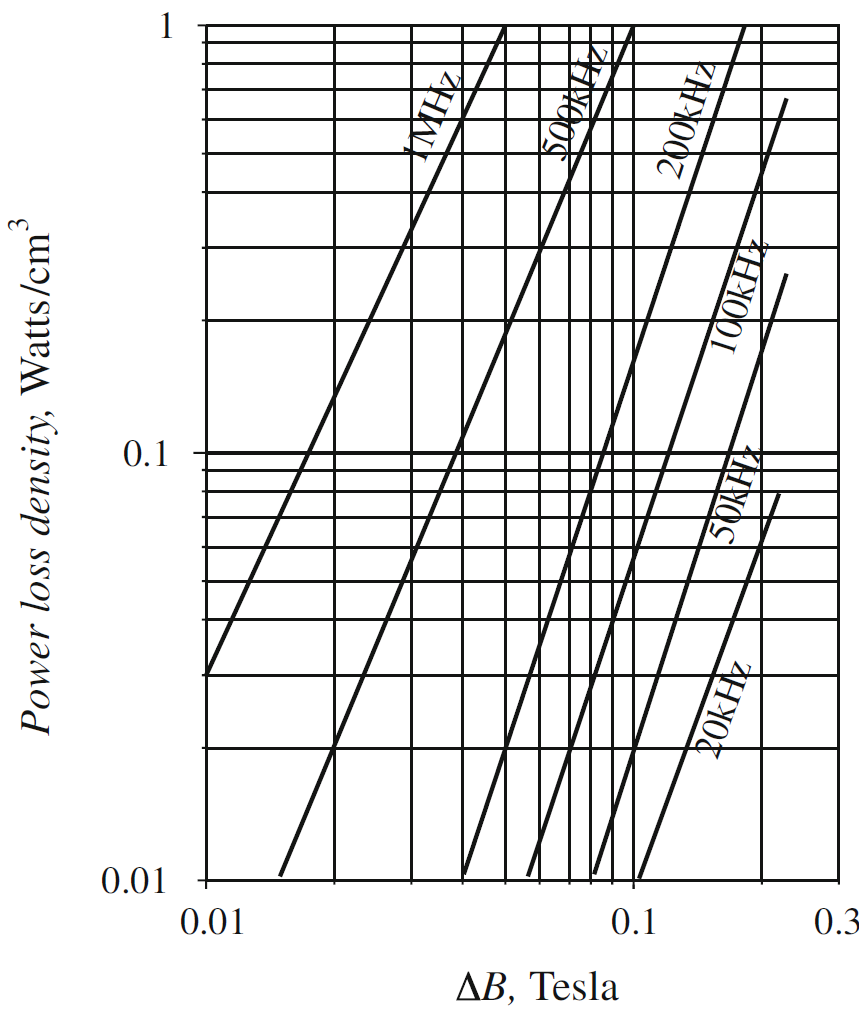
\includegraphics[width=0.65\linewidth]{fig/lec07/Ferrite_loss_curves.png} 
                \caption{Ferrite loss curves and comparison of magnetic materials. Adapted from Erickson \& Maksimović, \textit{Fundamentals of Power Electronics}, 3rd Edition.}
            \end{figure}
\end{column}
\end{columns}
\end{frame}


\begin{frame}{High-Frequency Copper Losses: Skin Effect and Proximity Effect}
At high switching frequencies, winding losses become considerably larger than their DC values.
The increase originates from two electromagnetic phenomena.
\begin{columns}
    \column{0.48\textwidth}
    \textbf{Skin Effect}
    \begin{itemize}
        \item Current crowds near the conductor surface.
        \item Effective conductor area decreases.
        \item AC resistance increases with frequency.
        \item Skin depth
        \[
        \delta=
        \sqrt{\frac{2\rho}{\omega\mu}}
        \]
        determines current penetration.
    \end{itemize}
\column{0.48\textwidth}
    \textbf{Proximity Effect}
    \begin{itemize}
        \item Magnetic fields generated by neighbouring conductors induce eddy currents.
        \item Current distribution becomes highly non-uniform.
        \item AC resistance increases further.
        \item Dominant in multilayer transformer windings.
    \end{itemize}
\end{columns}
\begin{block}{Practical Solution}
Use Litz wire, foil windings or interleaved winding arrangements to minimise AC copper losses.
\end{block}
\end{frame}


\begin{frame}{High-Frequency Copper Losses: Skin Effect and Proximity Effect}
    \begin{columns}
    \column{0.5\textwidth}
            \begin{figure} 
                \centering 
                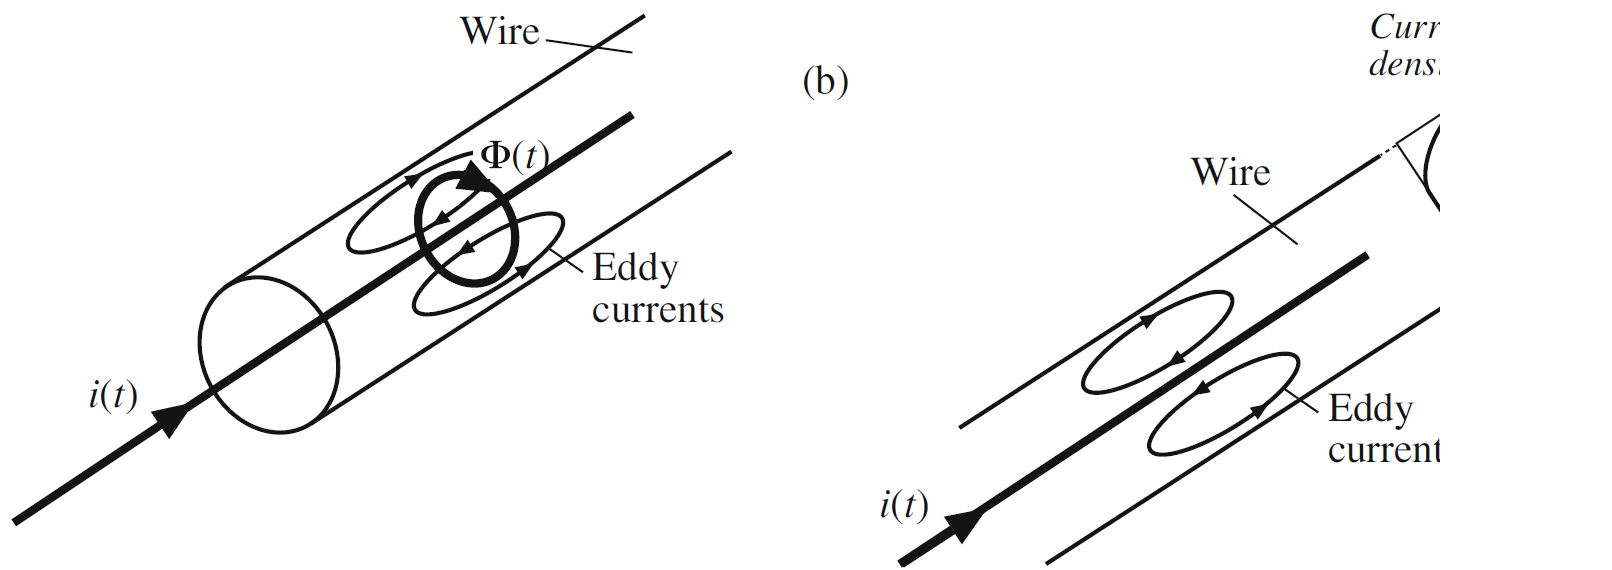
\includegraphics[width=0.9\linewidth]{fig/lec07/skin_effect.png} 
                \caption{Skin effect in conductors at high frequencies. Adapted from Erickson \& Maksimović, \textit{Fundamentals of Power Electronics}, 3rd Edition.}
            \end{figure} 

    \column{0.5\textwidth}
            \begin{figure} 
                \centering 
                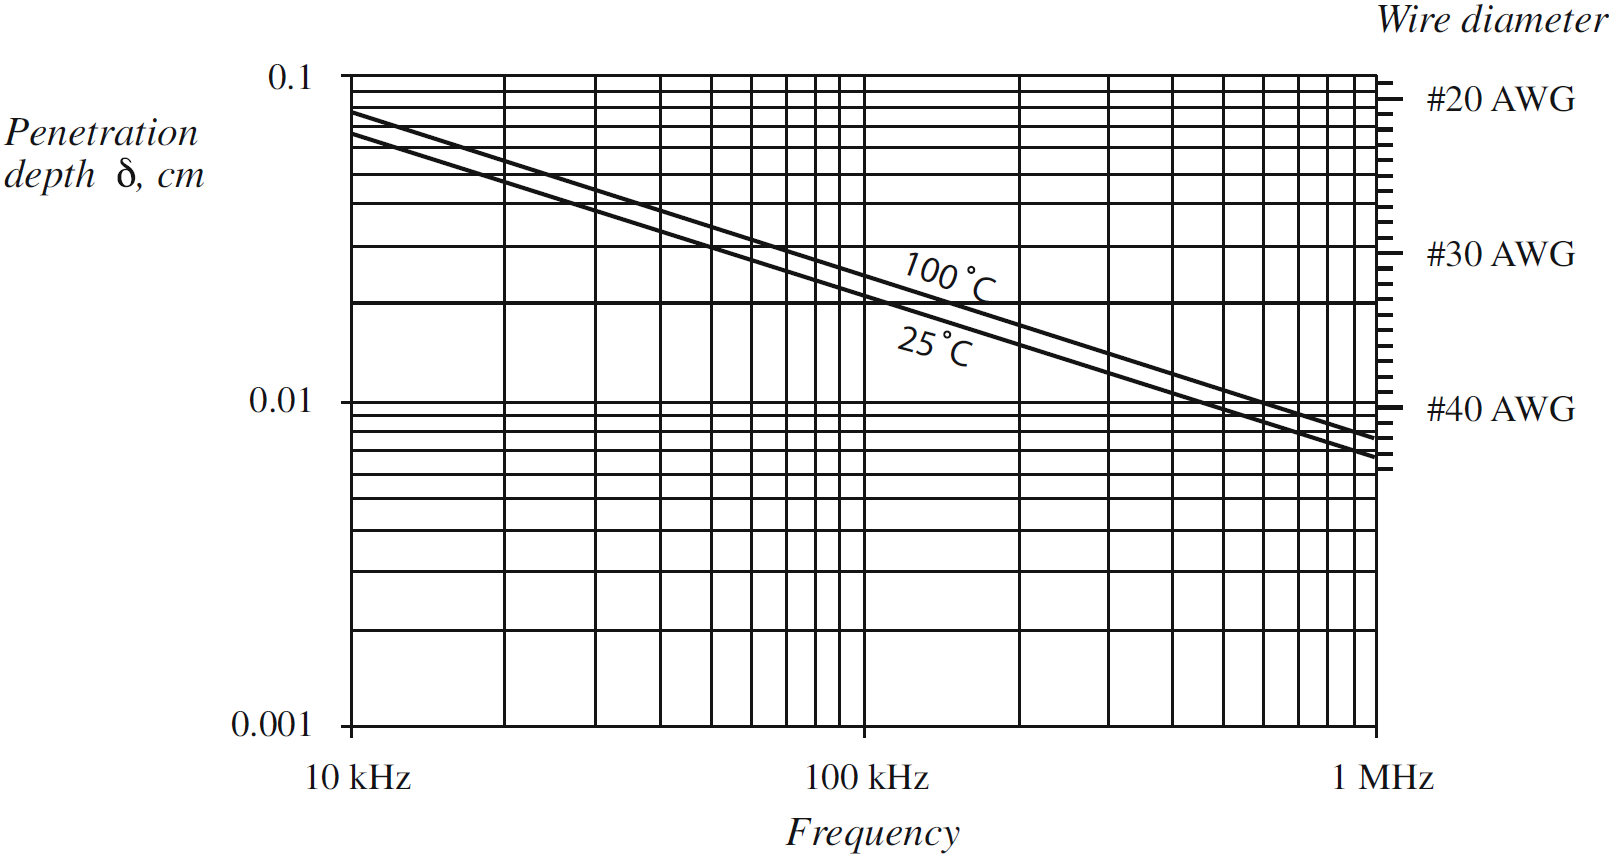
\includegraphics[width=0.9\linewidth]{fig/lec07/penetration_depth.png} 
                \caption{Penetration depth $\delta$ as a function of frequency $f$. Adapted from Erickson \& Maksimović, \textit{Fundamentals of Power Electronics}, 3rd Edition.}
            \end{figure} 
    \end{columns}
\end{frame}



\begin{frame}{High-Frequency Copper Losses: Skin Effect and Proximity Effect}
            \begin{figure} 
                \centering 
                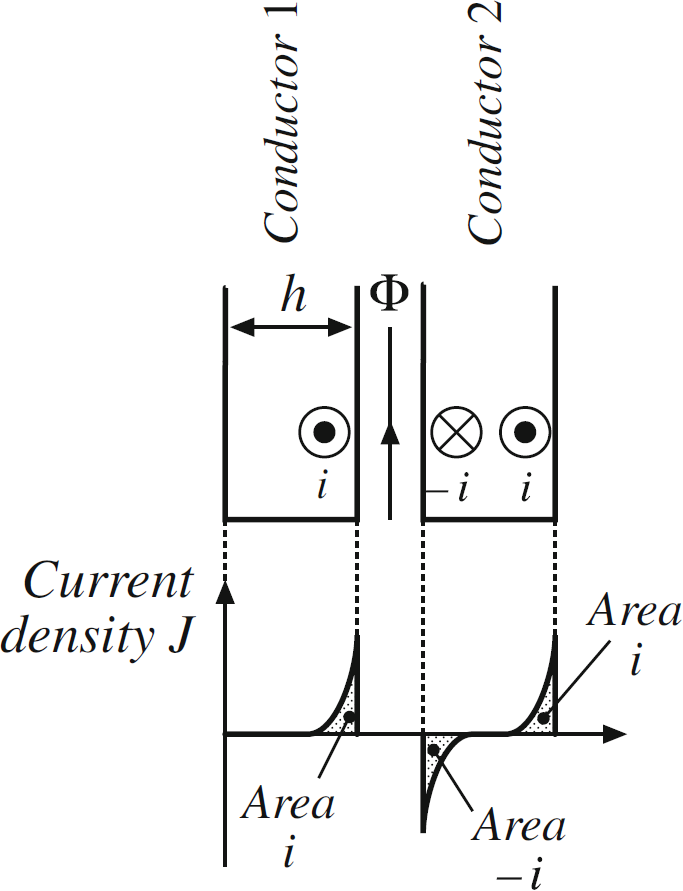
\includegraphics[width=0.275\linewidth]{fig/lec07/proximity_effect.png} 
                \caption{Proximity effect in conductors at high frequencies. Adapted from Erickson \& Maksimović, \textit{Fundamentals of Power Electronics}, 3rd Edition.}
            \end{figure} 
\end{frame}


\begin{frame}{Copper Loss versus Core Loss: Fundamental Design Trade-off}
Magnetic-component design always involves balancing copper loss and core loss.
\begin{columns}
\column{0.52\textwidth}
Increasing the allowable peak flux density $B_{\mathrm{pk}}$ produces
\begin{itemize}
\item fewer turns,
\item shorter winding length,
\item lower copper loss,
\item smaller magnetic component.
\end{itemize}
However,
\[
B_{\mathrm{pk}}
\uparrow
\Rightarrow
P_{\mathrm{core}}
\uparrow
\]
leading to higher temperature rise.
\column{0.44\textwidth}
\begin{block}{Design Objective}
Choose the operating flux density that minimises
\[
P_{\mathrm{total}}
=
P_{\mathrm{core}}
+
P_{\mathrm{copper}}
\]
rather than minimising either loss independently.
\end{block}
\end{columns}
\end{frame}

\begin{frame}{Copper Loss versus Core Loss: Fundamental Design Trade-off}
Magnetic-component design always involves balancing copper loss and core loss.
\begin{columns}
\column{0.3\textwidth}
\begin{alertblock}{Engineering Insight}
Modern GaN and SiC converters often operate at much higher switching frequencies.
Consequently, core loss usually becomes the dominant design constraint, while conventional
low-frequency converters are more frequently limited by copper loss.
\end{alertblock}
\column{0.6\textwidth}
            \begin{figure} 
                \centering 
                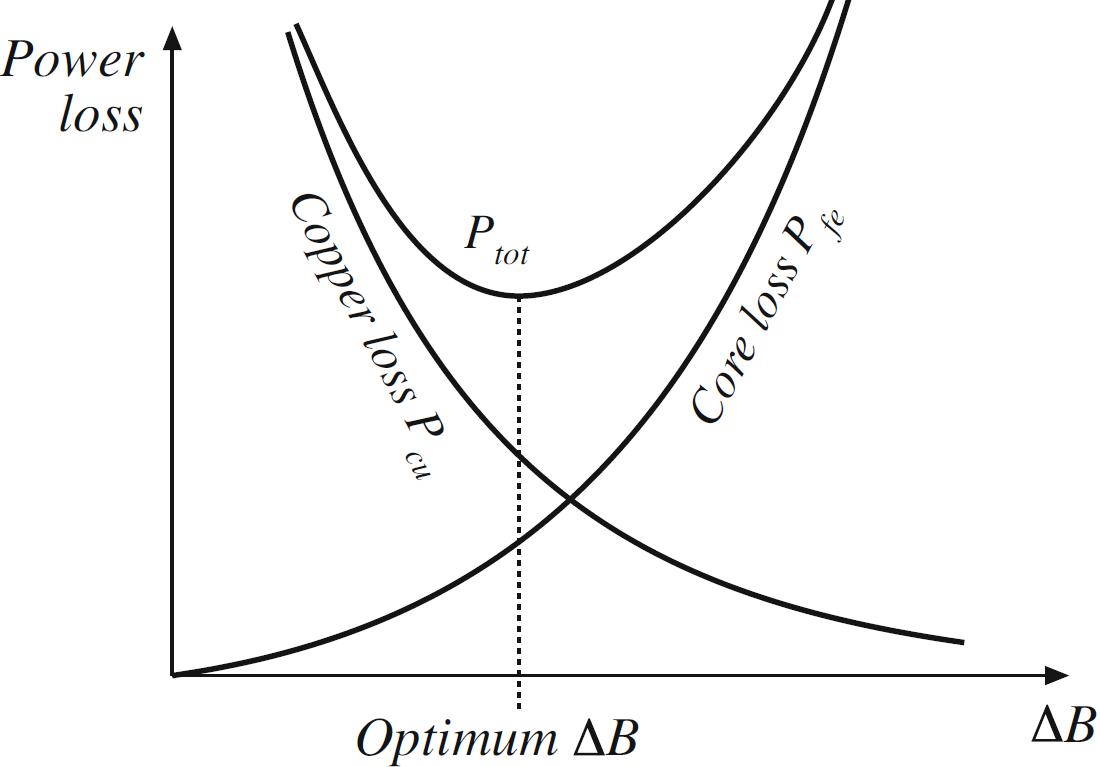
\includegraphics[width=0.8\linewidth]{fig/lec07/loss_curve.png} 
                \caption{Variation of copper loss, core loss and total loss versus peak flux density. Adapted from Erickson \& Maksimović, \textit{Fundamentals of Power Electronics}, 3rd Edition.}
            \end{figure} 
\end{columns}
\end{frame}


% %%%%%%%%%%%%%%%%%%%%%%%%%%%%%%%%%%%%%%%%%%%%%%%%%%%%%%%%%%%%% %% Air gap introduction %%%%%%%%%%%%%%%%%%%%%%%%%%%%%%%%%%%%%%%%%%%%%%%%%%%%%%%%%%%%% 
% \begin{frame} \frametitle{Why are Air Gaps Introduced in Inductors?} 
%     \begin{columns} 
%         \begin{column}{0.58\textwidth} 
%             Power inductors generally require an intentional air gap. 
%             \vspace{0.15cm} 
%             The air gap serves several important functions: 
%             \begin{itemize} 
%                 \item Increases magnetic reluctance. 
%                 \item Reduces effective permeability. 
%                 \item Increases saturation current. 
%                 \item Improves inductance stability. 
%                 \item Enables substantial energy storage. 
%             \end{itemize} 
%             \vspace{0.15cm} 
%             Without an air gap: 
%             \begin{itemize} 
%                 \item Flux density rises rapidly. 
%                 \item Core saturation occurs at relatively low current. 
%             \end{itemize} 
%         \end{column} 
%         \begin{column}{0.38\textwidth} 
%             \begin{figure} 
%                 \centering 
%                 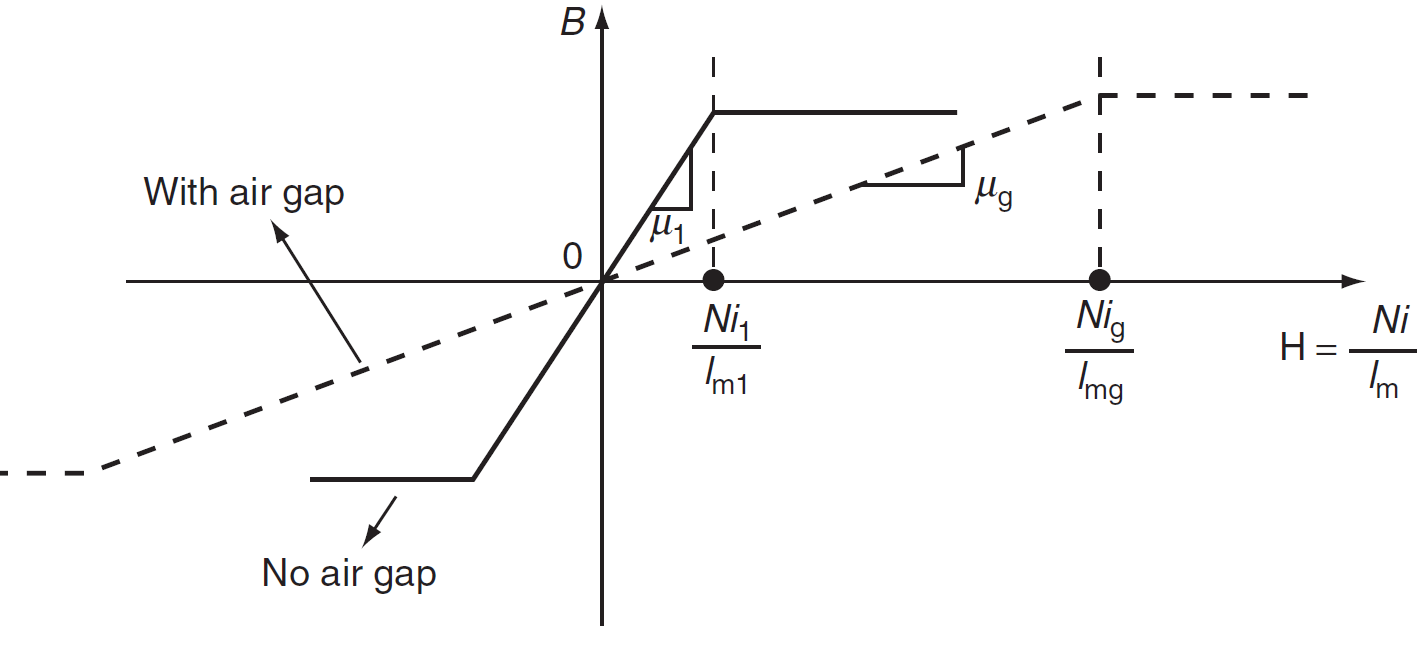
\includegraphics[width=\linewidth]{fig/lec07/air_gap_effect.png} 
%                 \caption{Influence of an air gap on the effective permeability and saturation behaviour. Adapted from Umanand, \textit{Power Electronics: Essentials and Applications}, 2nd edition, Wiley, 2012.}
%             \end{figure} 
%         \end{column} 
%     \end{columns} 
% \end{frame} 

% %%%%%%%%%%%%%%%%%%%%%%%%%%%%%%%%%%%%%%%%%%%%%%%%%%%%%%%%%%%%% %% Air gap and saturation %%%%%%%%%%%%%%%%%%%%%%%%%%%%%%%%%%%%%%%%%%%%%%%%%%%%%%%%%%%%%
% \begin{frame} 
%     \frametitle{Air Gap and Saturation Current} 
%     \begin{columns} 
%         \begin{column}{0.58\textwidth} 
%             The saturation condition occurs when 
%                 $B=B_{sat}$. Using $B=\mu H$ and $               H=\frac{Ni}{l_m} $ one obtains 
%             \begin{align} 
%                 i_{sat} \propto \frac{B_{sat}}{\mu} 
%             \end{align} 
%             \vspace{0.15cm} 
%             Introducing an air gap reduces the effective permeability. Therefore: 
%             \begin{itemize} 
%                 \item Flux density rises more slowly. 
%                 \item Larger current is required to reach saturation. 
%                 \item Energy-storage capability increases. 
%             \end{itemize} 
%         \end{column} 
%         \begin{column}{0.38\textwidth} 
%             \begin{block}{Design Trade-Off} Air gap: 
%                 \begin{itemize} 
%                     \item Higher saturation current 
%                     \item More energy storage 
%                     \item Lower inductance 
%                 \end{itemize} 
%             \end{block} 
%         \end{column} 
%     \end{columns} 
% \end{frame}


%%%%%%%%%%%%%%%%%%%%%%%%%%%%%%%%%%%%%%%%%%%%%%%%%%%%%%%%%%%%% %% Core geometries %%%%%%%%%%%%%%%%%%%%%%%%%%%%%%%%%%%%%%%%%%%%%%%%%%%%%%%%%%%%%
\begin{frame} \frametitle{Magnetic Core Geometries} 
    \begin{columns} 
        \begin{column}{0.56\textwidth} 
            Different core geometries offer different trade-offs in: \vspace{-0.5cm}
            \begin{itemize} 
                \item Winding area 
                \item Leakage flux 
                \item Manufacturability 
                \item Cooling 
                \item Cost 
            \end{itemize} 
            Common geometries include: 
            \begin{itemize} 
                \item EI cores, E cores, C cores, Toroidal cores, PQ cores 
            \end{itemize} 
            Selection depends on frequency, power level, and isolation requirements. 
        \end{column} 
        \begin{column}{0.40\textwidth} 
            \vspace{-1cm}
            \begin{figure} 
                \centering 
                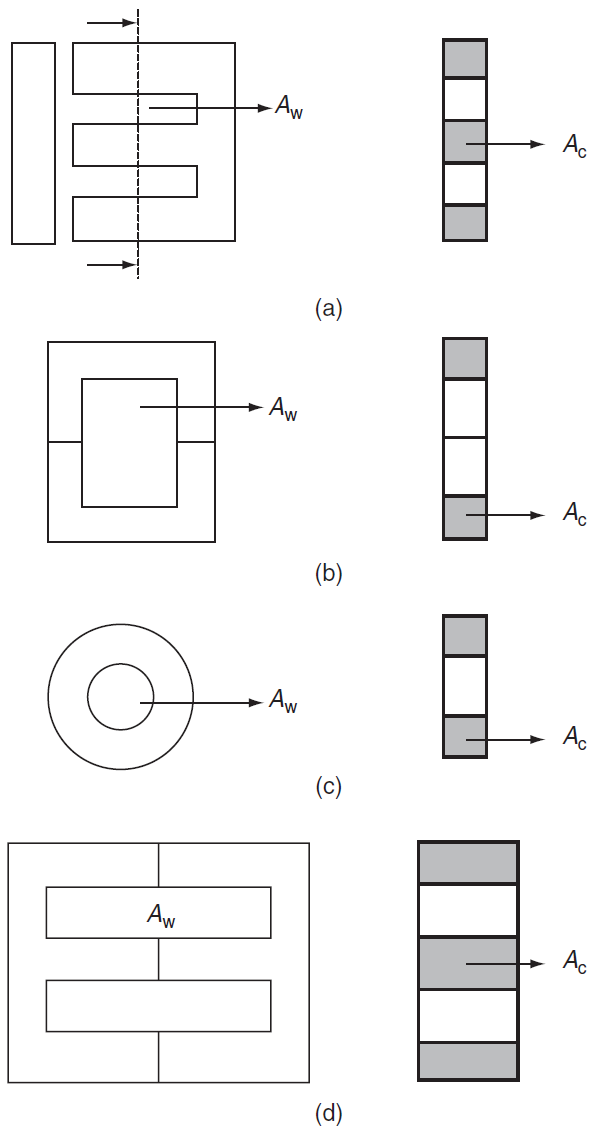
\includegraphics[height=0.68\textheight]{fig/lec07/core_geometries.png} 
                \caption{Window area and cross-sectional area for common magnetic-core geometries. Adapted from Umanand, \textit{Power Electronics: Essentials and Applications}, 2nd edition, Wiley, 2012.}
            \end{figure} 
        \end{column} 
    \end{columns} 
\end{frame} 

%%%%%%%%%%%%%%%%%%%%%%%%%%%%%%%%%%%%%%%%%%%%%%%%%%%%%%%%%%%%% %% Area product %%%%%%%%%%%%%%%%%%%%%%%%%%%%%%%%%%%%%%%%%%%%%%%%%%%%%%%%%%%%%
\begin{frame} 
    \frametitle{Area Product Concept} 
    \begin{columns} 
        \begin{column}{0.58\textwidth} 
            The area-product method provides a simple approach for selecting a magnetic core. 
            \vspace{0.15cm} Two physical parameters are particularly important: 
                $A_c$ 
            Core cross-sectional area and 
                $A_w$. 
            Window area available for windings. Their product 
            \begin{align} 
                A_P=A_cA_w 
            \end{align} is called the area product. 
            \vspace{0.15cm} It links the magnetic core dimensions directly to the electrical design requirements. 
        \end{column} 
        \begin{column}{0.38\textwidth} 
            \begin{block}{Interpretation} \[ A_c \] determines flux capability 
                \vspace{0.1cm} \[ A_w \] determines copper capability 
                \vspace{0.1cm} \[ A_P \] determines overall magnetic capability 
            \end{block} 
        \end{column} 
    \end{columns} 
\end{frame}

%%%%%%%%%%%%%%%%%%%%%%%%%%%%%%%%%%%%%%%%%%%%%%%%%%%%%%%%%%%%% %% Window area %%%%%%%%%%%%%%%%%%%%%%%%%%%%%%%%%%%%%%%%%%%%%%%%%%%%%%%%%%%%%
\begin{frame} \frametitle{Window Area and Copper Accommodation} 
    \begin{columns} 
        \begin{column}{0.58\textwidth} 
            The magnetic core must provide sufficient space to accommodate all winding conductors. 
            \vspace{0.15cm} The available winding space is called the window area: $A_w$. However, the entire window cannot be filled with copper because insulation, bobbins, air spaces, and manufacturing constraints occupy part of the available area. 
                \vspace{0.15cm} 
                Therefore, the usable copper area becomes 
                \begin{align} 
                    A_{Cu} = K_w A_w 
                \end{align} 
                where, $A_w$ = window area and $A_{Cu}$ = total copper area, and $K_w$ is the window utilization factor.
                \vspace{0.15cm} Typical values: $0.2 < K_w < 0.5$ depending on winding complexity. 
            \end{column} 
            \begin{column}{0.38\textwidth} 
                \vspace{-1cm}
                \begin{figure} 
                    \centering 
                    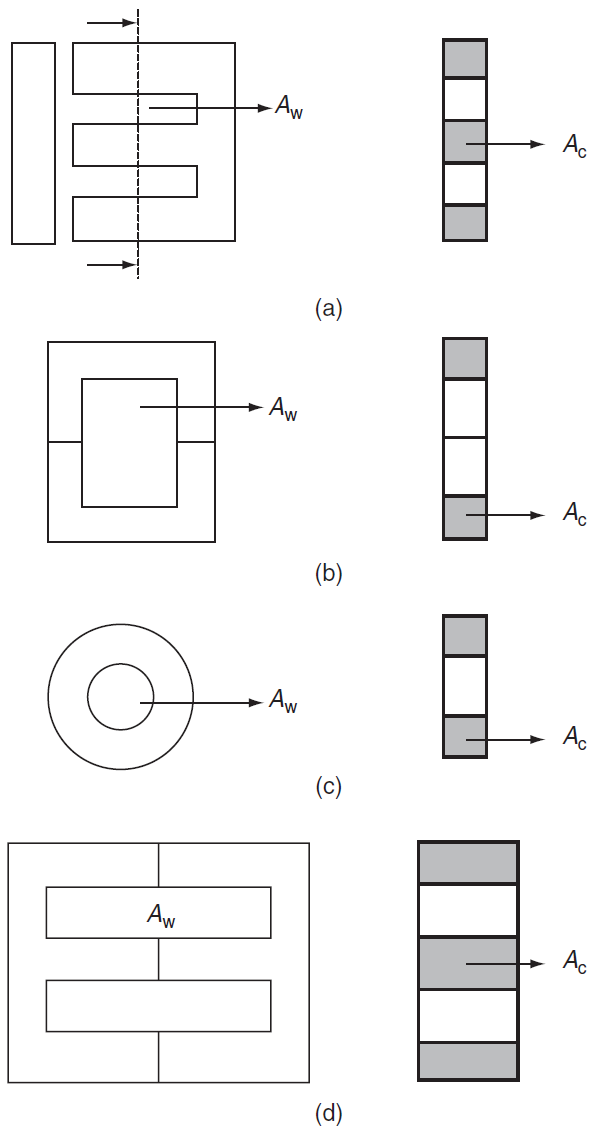
\includegraphics[height=0.68\textheight]{fig/lec07/core_geometries.png} 
                    \caption{Definition of window area $A_w$ and core cross-sectional area $A_c$. Adapted from Umanand, \textit{Power Electronics: Essentials and Applications}, 2nd edition, Wiley, 2012.}
                \end{figure} 
            \end{column} 
    \end{columns} 
\end{frame}

%%%%%%%%%%%%%%%%%%%%%%%%%%%%%%%%%%%%%%%%%%%%%%%%%%%%%%%%%%%%% %% Current density %%%%%%%%%%%%%%%%%%%%%%%%%%%%%%%%%%%%%%%%%%%%%%%%%%%%%%%%%%%%% 
\begin{frame} 
\frametitle{Current Density Constraint} 
\begin{columns} 
    \begin{column}{0.58\textwidth} 
        Conductor size is selected according to the allowable current density. 
        \vspace{0.15cm} 
        Current density is defined as 
        \begin{align} 
            J = \frac{I}{A_{wire}} 
        \end{align} 
        where 
        \begin{itemize} 
            \item $I$ is conductor current 
            \item $A_{wire}$ is conductor cross-sectional area 
        \end{itemize} 
        A high current density reduces winding size but increases: 
        \begin{itemize} 
            \item Copper loss 
            \item Temperature rise 
            \item Reliability concerns 
        \end{itemize} 
        \end{column} 
        \begin{column}{0.38\textwidth} 
            \begin{block}{Typical Values} 
                Power magnetics: 
                \begin{align} 
                    J = 3-6 \ \si{\ampere\per\milli\metre^2} 
                \end{align} 
                depending on cooling and thermal constraints. 
            \end{block} 
        \end{column} 
    \end{columns} 
\end{frame}

%%%%%%%%%%%%%%%%%%%%%%%%%%%%%%%%%%%%%%%%%%%%%%%%%%%%%%%%%%%%% %% Window area requirement %%%%%%%%%%%%%%%%%%%%%%%%%%%%%%%%%%%%%%%%%%%%%%%%%%%%%%%%%%%%%
\begin{frame} 
    \frametitle{Required Window Area for an Inductor} 
    \begin{columns} 
        \begin{column}{0.58\textwidth} 
            Assume an inductor consists of $N$ turns carrying current $I$. 
            \vspace{0.15cm} 
            The total conductor area required becomes 
                $A_{Cu} = N A_{wire}$.
            Using $A_{wire} = \frac{I}{J}$ gives
            \begin{align} 
                A_{Cu} = \frac{NI}{J} 
            \end{align} 
            Since 
            \begin{align} 
                A_{Cu} = K_w A_w 
            \end{align} 
            the required window area becomes 
            \begin{align} 
                A_w = \frac{NI}{J K_w} 
            \end{align} 
            This is the first key design equation of the area-product method. 
        \end{column} 
        \begin{column}{0.38\textwidth} 
            \begin{block}{Interpretation} Higher current: $\Rightarrow$ larger wire \vspace{0.1cm} More turns: $\Rightarrow$ larger window \vspace{0.1cm} Lower current density: $\Rightarrow$ larger magnetic core 
            \end{block} 
        \end{column} 
    \end{columns} 
\end{frame} 

%%%%%%%%%%%%%%%%%%%%%%%%%%%%%%%%%%%%%%%%%%%%%%%%%%%%%%%%%%%%% %% Flux density constraint %%%%%%%%%%%%%%%%%%%%%%%%%%%%%%%%%%%%%%%%%%%%%%%%%%%%%%%%%%%%% 
\begin{frame} \frametitle{Flux Density Constraint} 
    \begin{columns} 
        \begin{column}{0.58\textwidth} 
            The magnetic core must also satisfy the allowable flux-density limit. \vspace{0.15cm} The magnetic flux is 
            \begin{align} 
                \Phi = B_m A_c 
            \end{align} 
            where 
            \begin{itemize} 
                \item $B_m$ is maximum operating flux density 
                \item $A_c$ is core cross-sectional area \end{itemize} \vspace{0.15cm} The selected value of $B_m$ must remain below $B_{sat}$ to avoid saturation. In practice, 
                    \begin{align} 
                        B_m = 0.2-0.4B_{sat} 
                    \end{align} is commonly chosen to limit core loss and temperature rise. 
                \end{column} 
        \begin{column}{0.38\textwidth} 
                    \begin{block}{Design Rule} Large $B_m$ \vspace{0.05cm} $\Rightarrow$ smaller core \vspace{0.15cm} but \vspace{0.15cm} higher core loss \vspace{0.15cm} and smaller saturation margin. 
                    \end{block} 
        \end{column} 
    \end{columns} 
\end{frame} %%%%%%%%%%%%%%%%%%%%%%%%%%%%%%%%%%%%%%%%%%%%%%%%%%%%%%%%%%%%% %% Area product introduction %%%%%%%%%%%%%%%%%%%%%%%%%%%%%%%%%%%%%%%%%%%%%%%%%%%%%%%%%%%%%
\begin{frame} \frametitle{Derivation of the Area Product Method}
    \begin{columns} 
        \begin{column}{0.58\textwidth} 
            Two independent constraints must simultaneously be satisfied: \vspace{0.15cm} 
            \begin{enumerate} 
                \item Copper accommodation constraint 
                \item Magnetic flux-density constraint
            \end{enumerate} 
            Combining both constraints leads to the area-product concept 
            \begin{align} 
                A_P = A_cA_w 
            \end{align} where 
            \begin{itemize} 
                \item $A_c$ determines magnetic capability 
                \item $A_w$ determines copper capability
            \end{itemize} 
            \vspace{0.15cm} 
            The area product links electrical requirements directly to core dimensions. 
        \end{column} 
        \begin{column}{0.38\textwidth} 
            \begin{block}{Why Area Product?} Rather than solving for $A_c$ and $A_w$ individually, the designer first determines $A_P$ and then selects a suitable commercial core. 
            \end{block} 
        \end{column} 
    \end{columns} 
\end{frame} 
%%%%%%%%%%%%%%%%%%%%%%%%%%%%%%%%%%%%%%%%%%%%%%%%%%%%%%%%%%%%% %% Area product equation %%%%%%%%%%%%%%%%%%%%%%%%%%%%%%%%%%%%%%%%%%%%%%%%%%%%%%%%%%%%%
\begin{frame} \frametitle{Area Product Equation for Power Inductors} 
    \begin{columns} 
        \begin{column}{0.58\textwidth} 
            Combining the energy-storage requirement
            \begin{align} 
                E=\frac12LI^2 
            \end{align} with the window-area and flux-density constraints yields the well-known area-product equation.
            \vspace{0.15cm} For practical inductor design,
            \begin{align} 
                A_P = \frac{2E} {K_wK_cJB_m} 
            \end{align} where 
            \begin{itemize} 
                \item $K_w$ = window utilization factor 
                \item $K_c$ = waveform crest factor 
                \item $J$ = current density 
                \item $B_m$ = maximum flux density 
            \end{itemize} 
        \end{column} 
        \begin{column}{0.38\textwidth} 
            \begin{block}{Meaning} More stored energy $\uparrow E$ requires $\uparrow A_P$ and therefore a larger magnetic core. 
            \end{block} 
        \end{column} 
    \end{columns} 
\end{frame} 
%%%%%%%%%%%%%%%%%%%%%%%%%%%%%%%%%%%%%%%%%%%%%%%%%%%%%%%%%%%%% %% Core selection %%%%%%%%%%%%%%%%%%%%%%%%%%%%%%%%%%%%%%%%%%%%%%%%%%%%%%%%%%%%% 
\begin{frame} 
    \frametitle{Core Selection Using Area Product}
    \begin{columns} 
        \begin{column}{0.58\textwidth} 
            Once the required area product has been calculated,
            \begin{align} 
                A_P^{req} 
            \end{align} 
            the designer consults magnetic-core manufacturer catalogues. 
            \vspace{0.15cm} 
            The selected core must satisfy 
            \begin{align} 
                A_P^{core} > A_P^{req} 
            \end{align} 
            \vspace{0.15cm} Typical selection criteria:
            \begin{itemize} 
                \item Thermal performance 
                \item Core material 
                \item Available winding window 
                \item Manufacturing constraints 
                \item Cost 
            \end{itemize} 
        \end{column} 
        \begin{column}{0.38\textwidth} 
            \begin{block}{Important Observation} Area product provides only a first-order selection. \vspace{0.15cm} Detailed verification must still be performed afterwards. 
            \end{block} 
        \end{column} 
    \end{columns} 
\end{frame} 

%%%%%%%%%%%%%%%%%%%%%%%%%%%%%%%%%%%%%%%%%%%%%%%%%%%%%%%%%%%%% %% Design procedure %%%%%%%%%%%%%%%%%%%%%%%%%%%%%%%%%%%%%%%%%%%%%%%%%%%%%%%%%%%%% 
\begin{frame} 
    \frametitle{Practical Inductor Design Procedure} 
    Based on the area product method, the design process consists of the following steps: 
    \vspace{0.2cm}
     \begin{enumerate} 
        \item Specify inductance $L$ and maximum current $I$. 
        \item Determine required stored energy: \[ E=\frac12LI^2 \] 
        \item Calculate required area product. 
        \item Select magnetic core. 
        \item Determine air-gap length. 
        \item Calculate required turns. 
        \item Select conductor size. 
        \item Verify flux density and temperature rise. 
    \end{enumerate} 
    \vspace{0.2cm} 
    These steps form the basis of most industrial magnetic-component design workflows. 
\end{frame} 

%%%%%%%%%%%%%%%%%%%%%%%%%%%%%%%%%%%%%%%%%%%%%%%%%%%%%%%%%%%%% %% Fringing flux 
%%%%%%%%%%%%%%%%%%%%%%%%%%%%%%%%%%%%%%%%%%%%%%%%%%%%%%%%%%%%% 
\begin{frame} 
    \frametitle{Fringing Flux Around Air Gaps} 
    \begin{columns} 
        \begin{column}{0.58\textwidth} 
            The previous analysis assumed that magnetic flux remains confined within the core cross-sectional area.
            \vspace{0.15cm} In practice, flux spreads outward near the air gap. 
            \vspace{0.15cm} This phenomenon is called fringing flux. 
            \vspace{0.15cm} Consequences include:
            \begin{itemize} 
                \item Increased effective gap area 
                \item Reduced effective gap reluctance 
                \item Increased winding eddy-current loss 
                \item Localized heating 
            \end{itemize} 
            \vspace{0.15cm} Fringing becomes increasingly important in high-current and high-frequency inductors. 
        \end{column} 
        \begin{column}{0.38\textwidth} 
            \begin{block}{Practical Solution} 
                Avoid placing winding conductors directly adjacent to the air gap. 
                \vspace{0.15cm} Many commercial designs deliberately move the gap away from copper windings. 
            \end{block} 
        \end{column} 
    \end{columns} 
\end{frame}


%%%%%%%%%%%%%%%%%%%%%%%%%%%%%%%%%%%%%%%%%%%%%%%%%%%%%%%%%%%%% %% Inductor design summary %%%%%%%%%%%%%%%%%%%%%%%%%%%%%%%%%%%%%%%%%%%%%%%%%%%%%%%%%%%%%
\begin{frame} 
    \frametitle{Summary of Practical Inductor Design} 
    \begin{itemize} 
        \item The area-product method combines magnetic and copper constraints. 
        \item Window area determines winding capability. 
        \item Core area determines flux capability. 
        \item Air gaps enable practical energy storage. 
        \item Core selection is usually performed using the required area product. 
        \item Fringing flux must be considered in practical implementations. 
        \item Detailed design requires verification of:
        \begin{itemize} 
            \item Flux density 
            \item Saturation current 
            \item Copper loss 
            \item Core loss 
            \item Temperature rise 
        \end{itemize} 
    \end{itemize} 
\end{frame}


%%%%%%%%%%%%%%%%%%%%%%%%%%%%%%%%%%%%%%%%%%%%%%%%%%%%%%%%%%%%%
%% Transformer concept
%%%%%%%%%%%%%%%%%%%%%%%%%%%%%%%%%%%%%%%%%%%%%%%%%%%%%%%%%%%%%
\begin{frame}
    \frametitle{What is a Transformer?}
    \begin{columns}
        \begin{column}{0.58\textwidth}
            A transformer is a magnetic device that transfers electrical energy from one circuit to another through magnetic coupling.
            \vspace{0.15cm}
            Unlike inductors, transformers are ideally designed to transfer energy rather than store it.
            \vspace{0.15cm}
            Key functions include:
            \begin{itemize}
                \item Voltage step-up
                \item Voltage step-down
                \item Galvanic isolation
                \item Impedance matching
                \item Multiple output generation
            \end{itemize}
        \end{column}
        \begin{column}{0.38\textwidth}
            Transformer operation relies on:
            \begin{itemize}
                \item Amp\`ere's law
                \item Faraday's law
                \item Mutual magnetic coupling
            \end{itemize}
            \begin{block}{Fundamental Difference}
                Inductor:
                \[
                    \text{Store energy}
                \]
                \vspace{0.15cm}
                Transformer:
                \[
                    \text{Transfer energy}
                \]
            \end{block}
        \end{column}
    \end{columns}
\end{frame}


%%%%%%%%%%%%%%%%%%%%%%%%%%%%%%%%%%%%%%%%%%%%%%%%%%%%%%%%%%%%%
%% Ideal transformer
%%%%%%%%%%%%%%%%%%%%%%%%%%%%%%%%%%%%%%%%%%%%%%%%%%%%%%%%%%%%%
\begin{frame}
    \frametitle{Ideal Transformer Model}
    \begin{columns}
        \begin{column}{0.58\textwidth}
            The ideal transformer assumes:
            \begin{itemize}
                \item Infinite permeability
                \item Zero leakage flux
                \item Zero winding resistance
                \item Zero core loss
                \item Perfect magnetic coupling
            \end{itemize}
            Under these assumptions,
            \begin{align}
                \frac{v_1}{N_1} &= \frac{v_2}{N_2} \\
                \frac{i_1}{N_2} &= -\frac{i_2}{N_1}
            \end{align}
        \end{column}
        \begin{column}{0.38\textwidth}
            The negative sign reflects power conservation and dot-convention polarity.
            \begin{figure}
                \centering
                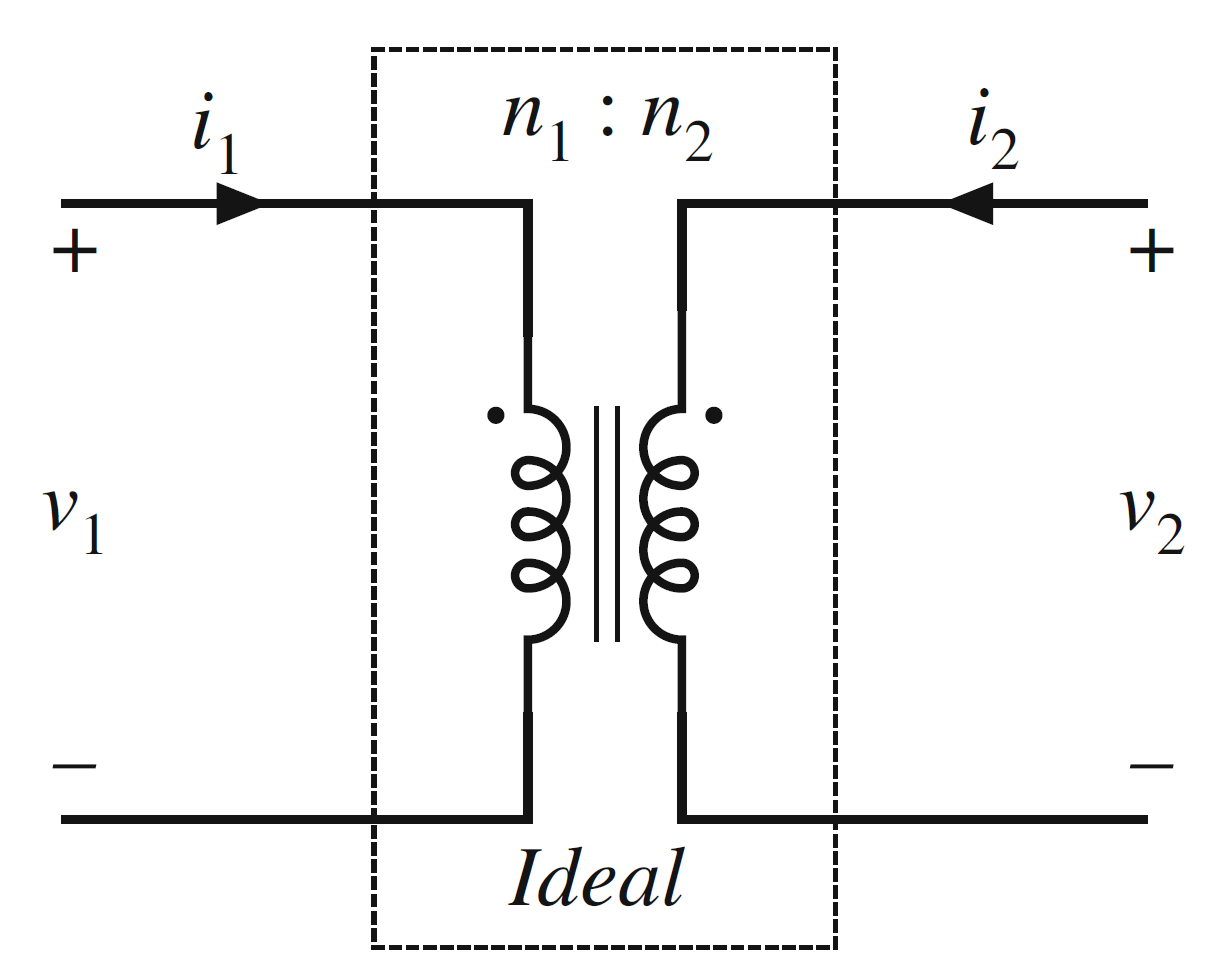
\includegraphics[width=0.7\linewidth]{fig/lec07/Ideal_Transformer_Model.png}
                \caption{Ideal transformer representation. Adapted from Erickson and Maksimovic, \textit{Fundamentals of Power Electronics}, 3rd edition, Springer, 2013.}
            \end{figure}
        \end{column}
    \end{columns}
\end{frame}


%%%%%%%%%%%%%%%%%%%%%%%%%%%%%%%%%%%%%%%%%%%%%%%%%%%%%%%%%%%%%
%% Voltage ratio
%%%%%%%%%%%%%%%%%%%%%%%%%%%%%%%%%%%%%%%%%%%%%%%%%%%%%%%%%%%%%
\begin{frame}
    \frametitle{Voltage Transformation Ratio}
    \begin{columns}
        \begin{column}{0.58\textwidth}
            Applying Faraday's law to both windings,
            \begin{align}
                v_1 &= N_1\frac{d\Phi}{dt}
            \end{align}
            \begin{align}
                v_2 &= N_2\frac{d\Phi}{dt}
            \end{align}
            Dividing the equations gives
            \begin{align}
                \frac{v_2}{v_1} &= \frac{N_2}{N_1}
            \end{align}
        \end{column}
        \begin{column}{0.38\textwidth}
            This relation determines whether the transformer acts as:
            \begin{itemize}
                \item Step-up transformer
                \item Step-down transformer
                \item Isolation transformer
            \end{itemize}
            \begin{block}{Example}
                $N_1=20$ and $N_2=100$
                \begin{equation}
                    \frac{V_2}{V_1}=5
                \end{equation}
                Voltage is increased by a factor of five.
            \end{block}
        \end{column}
    \end{columns}
\end{frame}


%%%%%%%%%%%%%%%%%%%%%%%%%%%%%%%%%%%%%%%%%%%%%%%%%%%%%%%%%%%%%
%% Current ratio
%%%%%%%%%%%%%%%%%%%%%%%%%%%%%%%%%%%%%%%%%%%%%%%%%%%%%%%%%%%%%
\begin{frame}
    \frametitle{Current Transformation Ratio}
    \begin{columns}
        \begin{column}{0.45\textwidth}
            Power conservation in an ideal transformer requires
            \begin{align}
                v_1 i_1 &= v_2 i_2
            \end{align}
            Using
            \begin{align}
                \frac{v_2}{v_1} &= \frac{N_2}{N_1}
            \end{align}
            gives
            \begin{align}
                \frac{i_2}{i_1} &= \frac{N_1}{N_2}
            \end{align}
        \end{column}
        \begin{column}{0.5\textwidth}
            \begin{block}{Design Insight}
                High-voltage winding $\Rightarrow$ low current \\
                Low-voltage winding $\Rightarrow$ high current
            \end{block}
            Important observations:
            \begin{itemize}
                \item Voltage increases with turns ratio.
                \item Current decreases with turns ratio.
                \item Power remains unchanged in the ideal case.
            \end{itemize}
        \end{column}
    \end{columns}
\end{frame}


%%%%%%%%%%%%%%%%%%%%%%%%%%%%%%%%%%%%%%%%%%%%%%%%%%%%%%%%%%%%%
%% Ampere turn balance
%%%%%%%%%%%%%%%%%%%%%%%%%%%%%%%%%%%%%%%%%%%%%%%%%%%%%%%%%%%%%
\begin{frame}
    \frametitle{Ampere-Turn Balance}
    \begin{columns}
        \begin{column}{0.58\textwidth}
            Applying Amp\`ere's law around the magnetic core yields
            \begin{align}
                N_1 i_1 + N_2 i_2 &= 0
            \end{align}
            This relation is called ampere-turn balance.
            \vspace{0.15cm}
            Physically:
            \begin{itemize}
                \item Primary current establishes flux.
                \item Secondary current opposes that flux.
                \item The core adjusts so that net flux remains finite.
            \end{itemize}
            \vspace{0.15cm}
            This is the magnetic equivalent of current balance in electrical circuits.
        \end{column}
        \begin{column}{0.38\textwidth}
            \begin{block}{Key Result}
                \begin{align}
                    N_1 i_1 &= -N_2 i_2
                \end{align}
                Ampere-turns cancel.
            \end{block}
        \end{column}
    \end{columns}
\end{frame}


%%%%%%%%%%%%%%%%%%%%%%%%%%%%%%%%%%%%%%%%%%%%%%%%%%%%%%%%%%%%%
%% Magnetizing current
%%%%%%%%%%%%%%%%%%%%%%%%%%%%%%%%%%%%%%%%%%%%%%%%%%%%%%%%%%%%%
\begin{frame}
    \frametitle{Magnetizing Current}
    \begin{columns}
        \begin{column}{0.58\textwidth}
            A practical transformer requires a finite current to establish magnetic flux. This current is called the magnetizing current. Using
            $L_m = \frac{N^2}{\mathcal R}$ the magnetizing current becomes
            \begin{align}
                i_m &= \frac{1}{L_m} \int v\,dt
            \end{align}
            \vspace{0.15cm}
            Magnetizing current:
            \begin{itemize}
                \item Exists even under no-load conditions.
                \item Establishes the required core flux.
                \item Is usually much smaller than load current.
            \end{itemize}
        \end{column}
        \begin{column}{0.38\textwidth}
            \begin{figure}
                \centering
                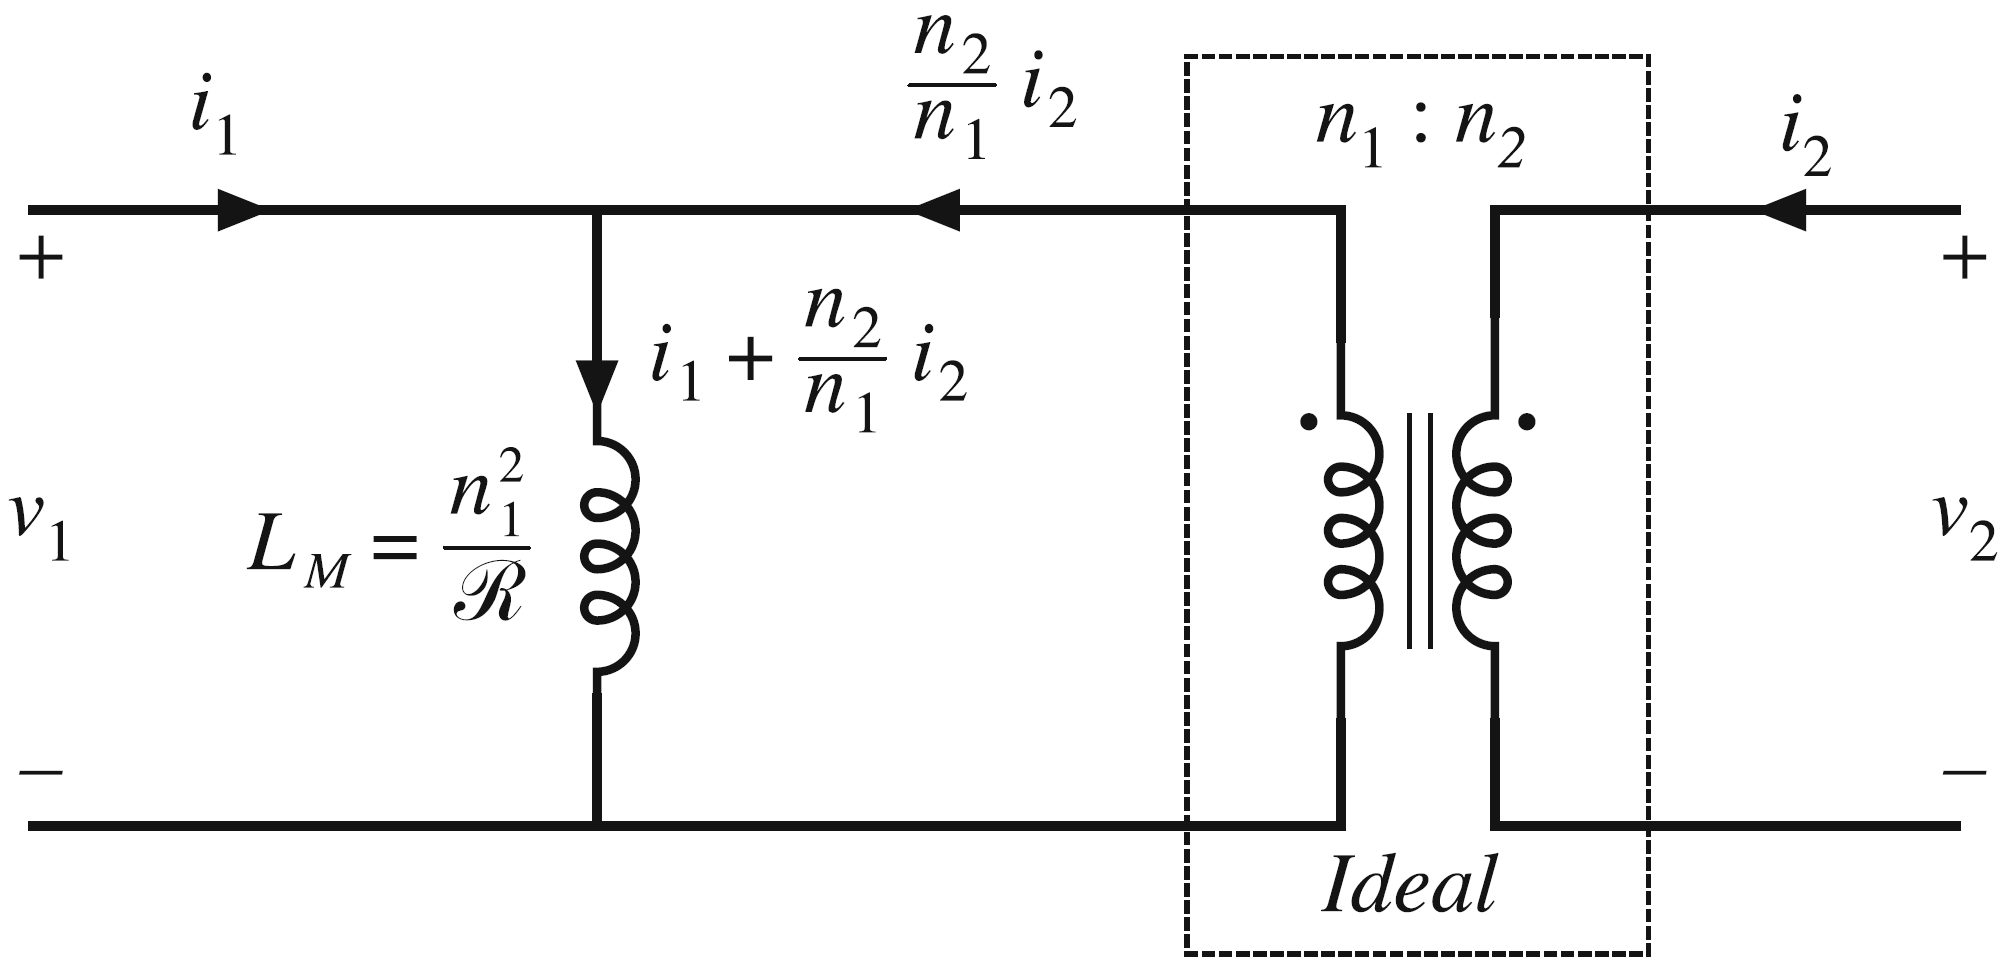
\includegraphics[width=\linewidth]{fig/lec07/Magnetizing_Inductance.png}
                \caption{Magnetizing inductance representation in a practical transformer. Adapted from Erickson and Maksimovic, \textit{Fundamentals of Power Electronics}, 3rd edition, Springer, 2013.}
            \end{figure}
        \end{column}
    \end{columns}
\end{frame}


%%%%%%%%%%%%%%%%%%%%%%%%%%%%%%%%%%%%%%%%%%%%%%%%%%%%%%%%%%%%%
%% Magnetizing inductance
%%%%%%%%%%%%%%%%%%%%%%%%%%%%%%%%%%%%%%%%%%%%%%%%%%%%%%%%%%%%%
\begin{frame}
    \frametitle{Physical Meaning of Magnetizing Inductance}
    \begin{columns}
        \begin{column}{0.58\textwidth}
            Magnetizing inductance represents the ability of the transformer core to establish magnetic flux.
            \vspace{0.15cm}
            \begin{align}
                L_m &= \frac{N^2}{\mathcal R}
            \end{align}
            Therefore,
            \begin{itemize}
                \item Higher permeability increases $L_m$.
                \item More turns increase $L_m$.
                \item Air gaps reduce $L_m$.
                \item Lower reluctance increases $L_m$.
            \end{itemize}
            \vspace{0.15cm}
            Power transformers generally seek a large magnetizing inductance to minimize no-load current.
        \end{column}
        \begin{column}{0.38\textwidth}
            \begin{block}{Transformer Design Goal}
                Large
                \begin{equation}
                    L_m
                \end{equation}
                \vspace{0.15cm}
                Small
                \begin{equation}
                    i_m
                \end{equation}
                \vspace{0.15cm}
                High efficiency
            \end{block}
        \end{column}
    \end{columns}
\end{frame}


%%%%%%%%%%%%%%%%%%%%%%%%%%%%%%%%%%%%%%%%%%%%%%%%%%%%%%%%%%%%%
%% Practical transformer
%%%%%%%%%%%%%%%%%%%%%%%%%%%%%%%%%%%%%%%%%%%%%%%%%%%%%%%%%%%%%
\begin{frame}
    \frametitle{Practical Transformer Equivalent Circuit}
    \begin{columns}
        \begin{column}{0.58\textwidth}
            Real transformers deviate from the ideal model because of:
            \begin{itemize}
                \item Copper resistance
                \item Leakage inductance
                \item Core loss
                \item Finite permeability
            \end{itemize}
            \vspace{0.15cm}
            The practical transformer therefore includes:
            \begin{itemize}
                \item Winding resistances
                \item Magnetizing inductance
                \item Core-loss resistance
                \item Leakage inductances
            \end{itemize}
            \vspace{0.15cm}
        \end{column}
        \begin{column}{0.38\textwidth}
            \begin{figure}
                \centering
                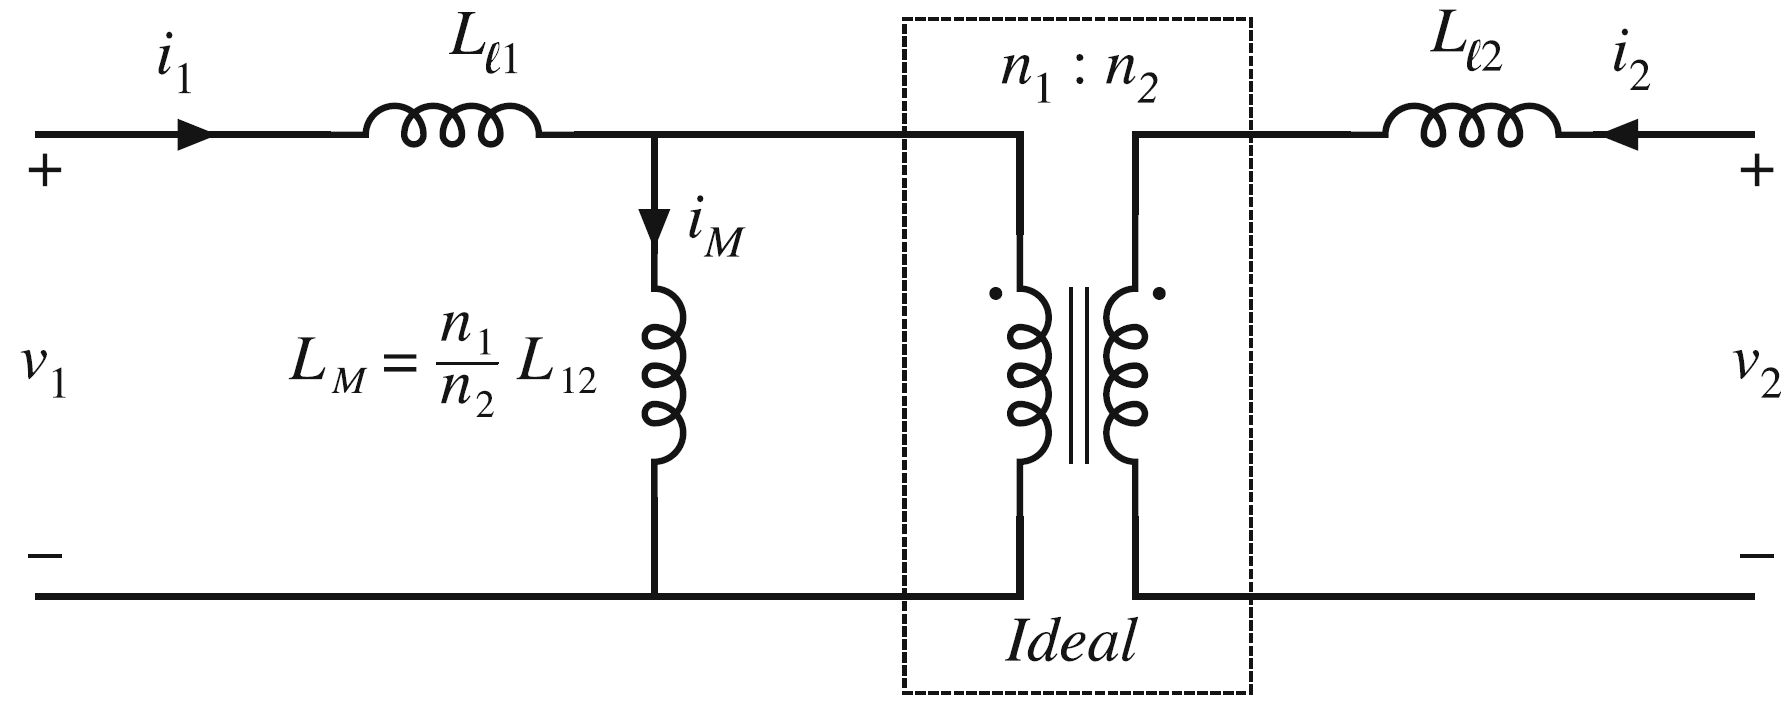
\includegraphics[width=\linewidth]{fig/lec07/Practical_Transformer_Equivalent.png}
                \caption{Practical transformer equivalent circuit including magnetizing branch and parasitic elements. Adapted from Erickson and Maksimovic, \textit{Fundamentals of Power Electronics}, 3rd edition, Springer, 2013.}
            \end{figure}
            This equivalent circuit is extensively used in transformer design and simulation.
        \end{column}
    \end{columns}
\end{frame}



% Next I should prepare slides on design of transformers including current transformers, then I want to talk about the losses, then I want to talk about the new versions like planer magnetics, MHz magnetics, and then I want to talk about the design of magnetic components for high frequency applications. Also, if possible something in direction of winding arrangements and cooling. This will conclude the magnetics. 


%%%%%%%%%%%%%%%%%%%%%%%%%%%%%%%%%%%%%%%%%%%%%%%%%%%%%%%%%%%%%
%% Practical magnetic components
%%%%%%%%%%%%%%%%%%%%%%%%%%%%%%%%%%%%%%%%%%%%%%%%%%%%%%%%%%%%%
\begin{frame}
\begin{center}
  \textbf{\Huge{Practical Magnetic Components}}\\[0.4cm]
  \textbf{\Large{Inductors, Transformers, Coupled Inductors, and Current Transformers}}
\end{center}
\end{frame}


%%%%%%%%%%%%%%%%%%%%%%%%%%%%%%%%%%%%%%%%%%%%%%%%%%%%%%%%%%%%%
%% Magnetic component families
%%%%%%%%%%%%%%%%%%%%%%%%%%%%%%%%%%%%%%%%%%%%%%%%%%%%%%%%%%%%%
\begin{frame}
    \frametitle{Main Families of Magnetic Components in Power Electronics}
    \begin{columns}
        \begin{column}{0.58\textwidth}
            Magnetic components in power electronics can be grouped according to their dominant function.

            \vspace{0.15cm}

            \begin{itemize}
                \item \textbf{Energy-storage components}
                \begin{itemize}
                    \item DC filter inductors
                    \item AC inductors or line reactors
                    \item Flyback magnetic components
                \end{itemize}

                \item \textbf{Energy-transfer components}
                \begin{itemize}
                    \item High-frequency transformers
                    \item Pulse transformers
                    \item Current transformers
                \end{itemize}

                \item \textbf{Coupled and integrated components}
                \begin{itemize}
                    \item Coupled inductors
                    \item Integrated magnetics
                    \item Planar magnetics
                \end{itemize}
            \end{itemize}
        \end{column}

        \begin{column}{0.38\textwidth}
            The correct magnetic component is selected from converter function, isolation requirement, stored energy, frequency, current ripple, and thermal constraints.
            \begin{block}{Key Design Question}
                Is the component mainly required to store energy, transfer energy, sense current, or combine several magnetic functions?
            \end{block}
        \end{column}
    \end{columns}
\end{frame}


%%%%%%%%%%%%%%%%%%%%%%%%%%%%%%%%%%%%%%%%%%%%%%%%%%%%%%%%%%%%%
%% Filter inductor
%%%%%%%%%%%%%%%%%%%%%%%%%%%%%%%%%%%%%%%%%%%%%%%%%%%%%%%%%%%%%
\begin{frame}
    \frametitle{Filter Inductor}

    \begin{columns}
        \begin{column}{0.58\textwidth}
            A filter inductor is used to control current ripple and shape the current waveform in a switching converter. Typical applications include:
            \begin{itemize}
                \item Buck converter output filter
                \item Boost converter input inductor
                \item PFC boost inductor
                \item DC-link filtering
                \item EMI and differential-mode filtering
            \end{itemize}
            The governing relation is
            \begin{align}
                v_L = L\frac{di_L}{dt}
            \end{align}
            A larger inductance reduces ripple, but also increases volume, copper loss, and stored energy requirement.
        \end{column}

        \begin{column}{0.38\textwidth}
            \begin{block}{Design Focus}
                \small
                For a filter inductor, the most important quantities are:
                \begin{itemize}
                    \item Required inductance $L$
                    \item Peak current $I_{\mathrm{pk}}$
                    \item RMS current $I_{\mathrm{rms}}$
                    \item Allowed ripple $\Delta i$
                    \item Saturation current
                    \item Temperature rise
                \end{itemize}
            \end{block}
        \end{column}
    \end{columns}
\end{frame}


%%%%%%%%%%%%%%%%%%%%%%%%%%%%%%%%%%%%%%%%%%%%%%%%%%%%%%%%%%%%%
%% AC inductor
%%%%%%%%%%%%%%%%%%%%%%%%%%%%%%%%%%%%%%%%%%%%%%%%%%%%%%%%%%%%%
\begin{frame}
    \frametitle{AC Inductor or Line Reactor}
    \begin{columns}
        \begin{column}{0.58\textwidth}
            An AC inductor, often called a line reactor, is used when the current is alternating rather than purely DC with ripple. It is commonly used in:
            \begin{itemize}
                \item Grid-connected converters
                \item Three-phase rectifiers
                \item Motor-drive output filters
                \item Active front-end converters
                \item LCL filters for inverters
            \end{itemize}
            Unlike a DC filter inductor, an AC inductor experiences bidirectional flux swing. So, the design must consider:
            \begin{itemize}
                \item Fundamental-frequency current
                \item Switching-frequency ripple
                \item Core loss under AC excitation
                \item Audible noise and vibration
            \end{itemize}
        \end{column}

        \begin{column}{0.38\textwidth}
            \begin{block}{Practical Difference}
                A DC filter inductor is often limited by peak current and saturation. An AC inductor is often limited by combined copper loss, core loss, thermal rise, and insulation stress.
            \end{block}
        \end{column}
    \end{columns}
\end{frame}


%%%%%%%%%%%%%%%%%%%%%%%%%%%%%%%%%%%%%%%%%%%%%%%%%%%%%%%%%%%%%
%% Coupled inductor
%%%%%%%%%%%%%%%%%%%%%%%%%%%%%%%%%%%%%%%%%%%%%%%%%%%%%%%%%%%%%
\begin{frame}
    \frametitle{Coupled Inductor}

    \begin{columns}
        \begin{column}{0.58\textwidth}
            A coupled inductor contains two or more windings on a common magnetic core. The windings share part of their magnetic flux. The coupling is described by the mutual inductance $M$ and the coupling coefficient $k$:
            \begin{align}
                k = \frac{M}{\sqrt{L_1L_2}}, \qquad 0 \leq k \leq 1
            \end{align}
            Coupled inductors are useful in:
            \begin{itemize}
                \item Interleaved buck converters
                \item Multiphase voltage regulators
                \item Coupled-inductor boost converters
                \item Ripple-current cancellation
                \item Integrated magnetic structures
            \end{itemize}

        \end{column}

        \begin{column}{0.38\textwidth}
            \begin{figure}
                \centering
                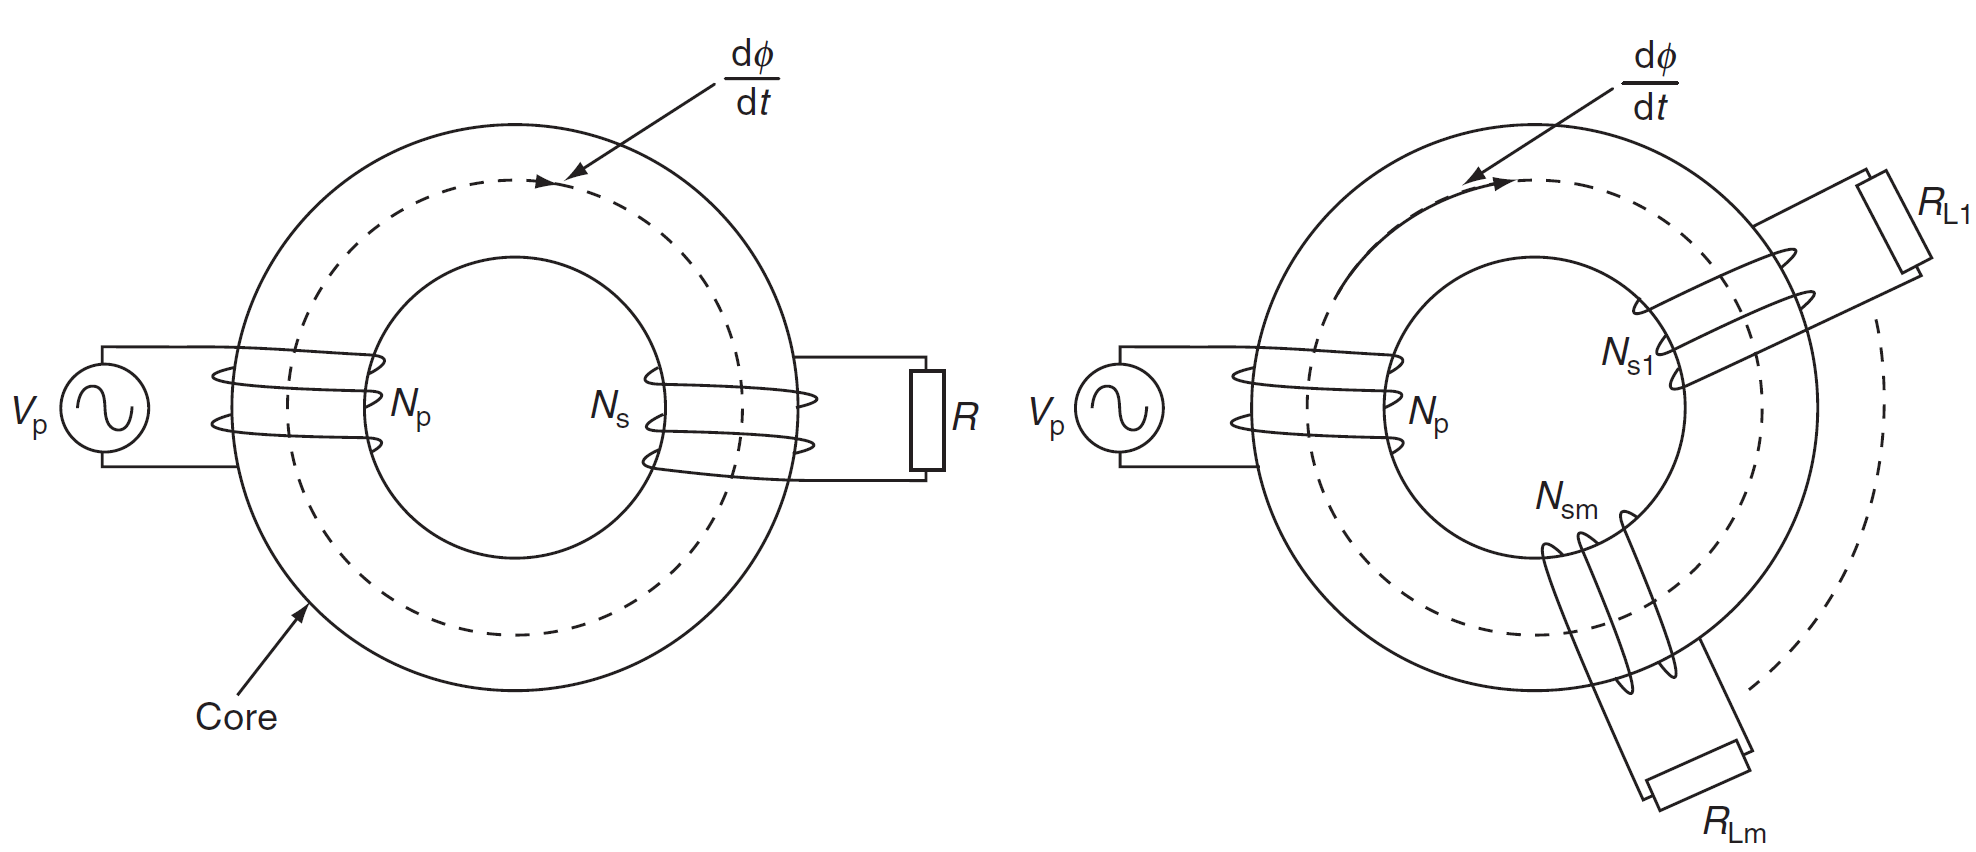
\includegraphics[width=\linewidth]{fig/lec07/coupled_inductor_ill.png}
                \caption{Multiple-winding magnetic structure illustrating shared magnetic coupling. Adapted from Umanand, \textit{Power Electronics: Essentials and Applications}}
            \end{figure}
        \end{column}
    \end{columns}
\end{frame}

%%%%%%%%%%%%%%%%%%%%%%%%%%%%%%%%%%%%%%%%%%%%%%%%%%%%%%%%%%%%%
%% Coupled inductor
%%%%%%%%%%%%%%%%%%%%%%%%%%%%%%%%%%%%%%%%%%%%%%%%%%%%%%%%%%%%%
\begin{frame}
    \frametitle{Coupled Inductor}

    \begin{columns}
        \begin{column}{0.58\textwidth}
            As in the case of the single winding filter inductor, the size of the minor B-H loop is proportional to the total current ripple (Fig. 10.48). Small ripple implies small core loss, as well as small proximity loss. An air gap is employed, and the maximum flux density is typically limited by saturation.
        \end{column}

        \begin{column}{0.38\textwidth}
            \begin{figure}
                \centering
                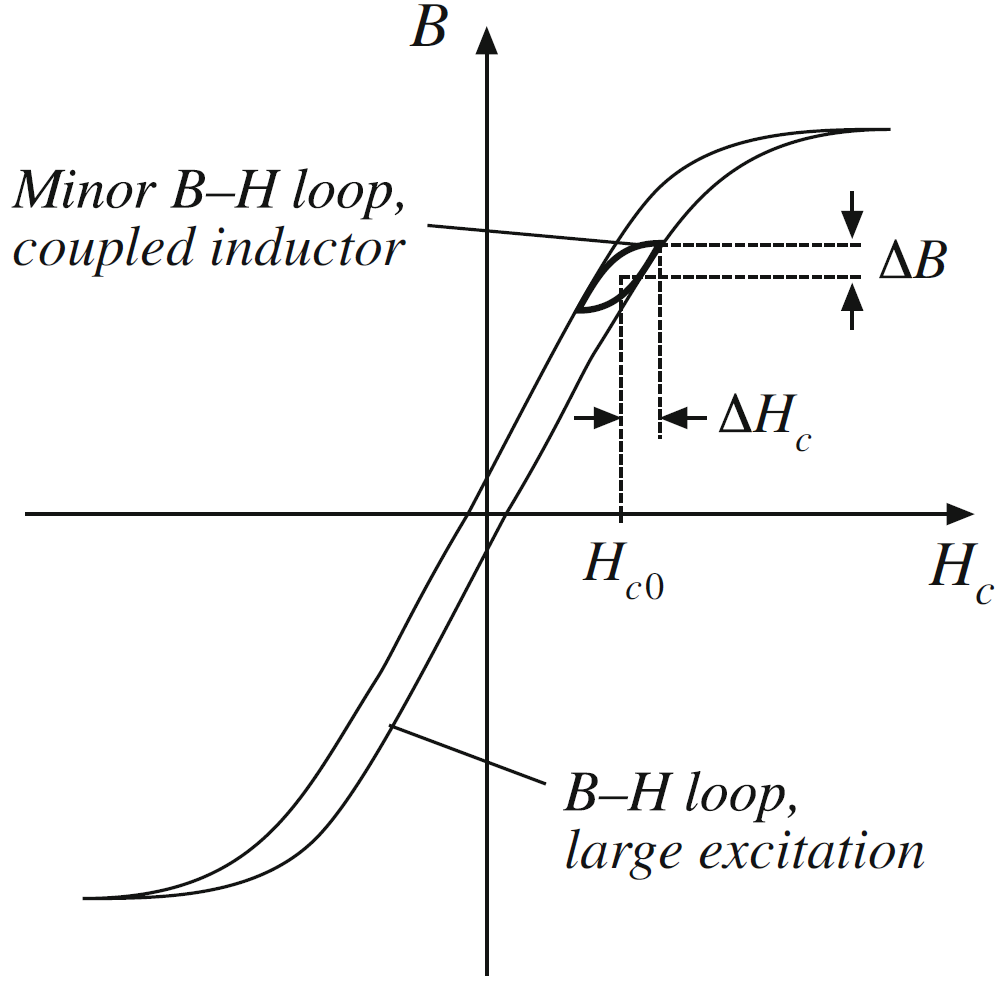
\includegraphics[width=0.8\linewidth]{fig/lec07/coupled_inductor.png}
                \caption{Coupled inductor minor B-H loop. Adapted from Errikson and Maksimovic, \textit{Fundamentals of Power Electronics}, 3rd edition, Springer, 2013}
            \end{figure}
        \end{column}
    \end{columns}
\end{frame}


%%%%%%%%%%%%%%%%%%%%%%%%%%%%%%%%%%%%%%%%%%%%%%%%%%%%%%%%%%%%%
%% True transformer
%%%%%%%%%%%%%%%%%%%%%%%%%%%%%%%%%%%%%%%%%%%%%%%%%%%%%%%%%%%%%
\begin{frame}
    \frametitle{High-Frequency Transformer}
    \begin{columns}
        \begin{column}{0.58\textwidth}
            A high-frequency transformer transfers energy between two or more electrical ports through a shared magnetic flux. It is used for:
            \begin{itemize}
                \item Galvanic isolation
                \item Voltage step-up or step-down
                \item Impedance matching
                \item Multiple isolated outputs
            \end{itemize}
            Applying Faraday's law to two windings gives
            \begin{align}
                \frac{v_1}{N_1} = \frac{v_2}{N_2}
            \end{align}

            and ideal ampere-turn balance gives

            \begin{align}
                N_1 i_1 + N_2 i_2 = 0
            \end{align}
        \end{column}

        \begin{column}{0.38\textwidth}
            A true transformer should ideally transfer energy, not store significant energy.
            \begin{figure}
                \centering
                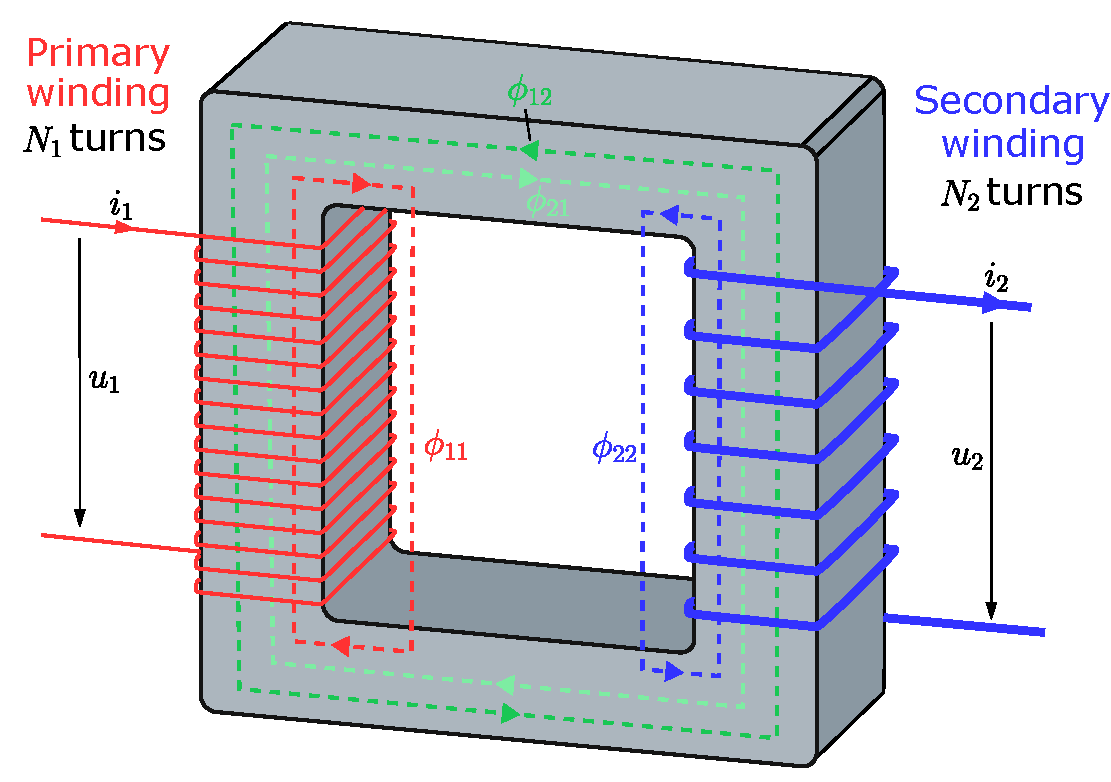
\includegraphics[width=\linewidth]{fig/lec07/Transformer3d_col3.pdf}
                \caption{Operating principle of a transformer with primary and secondary windings linked by common flux.}
            \end{figure}
        \end{column}
    \end{columns}
\end{frame}


%%%%%%%%%%%%%%%%%%%%%%%%%%%%%%%%%%%%%%%%%%%%%%%%%%%%%%%%%%%%%
%% Flyback transformer
%%%%%%%%%%%%%%%%%%%%%%%%%%%%%%%%%%%%%%%%%%%%%%%%%%%%%%%%%%%%%
\begin{frame}
    \frametitle{Flyback Transformer: Actually a Coupled Inductor}
    \begin{columns}
        \begin{column}{0.58\textwidth}
            The term ``flyback transformer'' is widely used in industry, but magnetically it is more accurately a coupled inductor. In a true transformer:
            \begin{itemize}
                \item Primary and secondary currents flow simultaneously.
                \item Ampere-turns largely cancel.
                \item Energy storage is undesirable.
            \end{itemize}
            In a flyback magnetic component:
            \begin{itemize}
                \item Primary and secondary currents occur sequentially.
                \item Energy is first stored in magnetizing inductance.
                \item Energy is later delivered to the secondary.
                \item An air gap is essential for energy storage.
            \end{itemize}
            \begin{align}
                E = \frac{1}{2}L_m I_{\mathrm{pk}}^2
            \end{align}
        \end{column}
        \begin{column}{0.38\textwidth}
            \vspace{-1cm}
            \begin{figure}
                \centering
                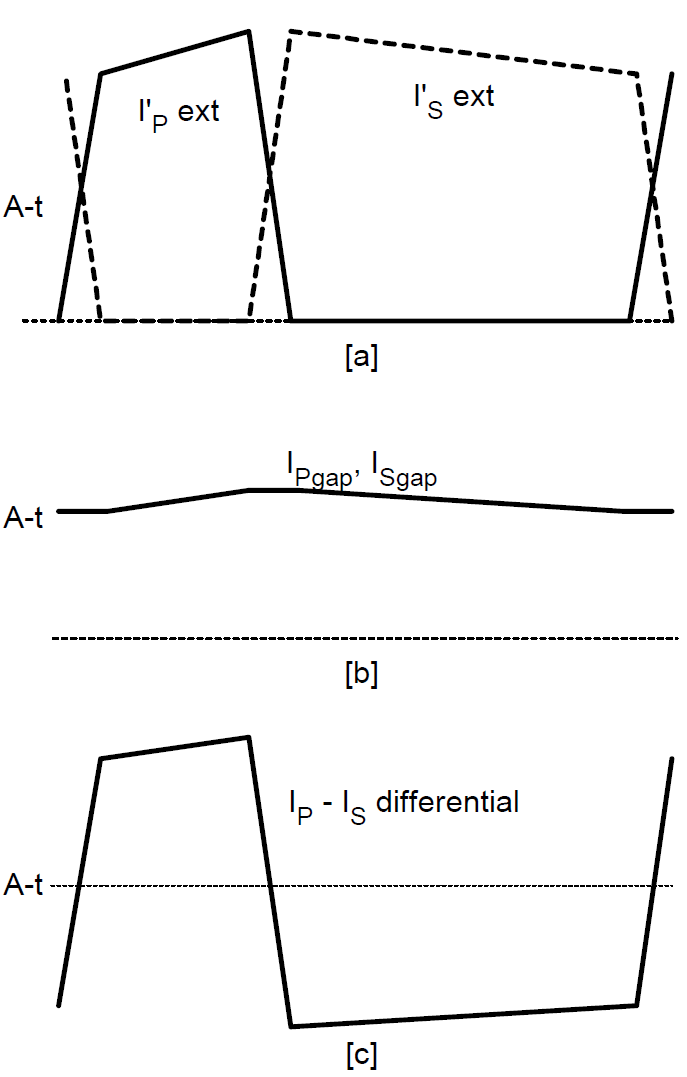
\includegraphics[width=0.6\linewidth]{fig/lec07/flyback_inductor.png}
                \caption{Continuous-mode flyback winding ampere-turn waveforms showing sequential primary and secondary current action. Adapted from Dixon, Texas Instruments, \textit{Designing Planar Magnetics}}
            \end{figure}
        \end{column}
    \end{columns}
\end{frame}


%%%%%%%%%%%%%%%%%%%%%%%%%%%%%%%%%%%%%%%%%%%%%%%%%%%%%%%%%%%%%
%% Current transformer
%%%%%%%%%%%%%%%%%%%%%%%%%%%%%%%%%%%%%%%%%%%%%%%%%%%%%%%%%%%%%
\begin{frame}
    \frametitle{Current Transformer}
    \begin{columns}
        \begin{column}{0.58\textwidth}
            A current transformer is a magnetic sensor used to reproduce a scaled version of a primary current in an isolated secondary circuit. For an ideal current transformer,
            \begin{align}
                \frac{I_s}{I_p} \approx \frac{N_p}{N_s}
            \end{align}
            Typical uses include:
            \begin{itemize}
                \item Isolated current sensing
                \item Over-current protection
                \item Gate-drive power sensing
                \item Converter diagnostics
                \item Protection relays
            \end{itemize}

        \end{column}
        \begin{column}{0.38\textwidth}
            The secondary current is usually converted to a voltage using a burden resistor:
            \begin{align}
                v_s = I_s R_b
            \end{align}
            \vspace{-0.75cm}
            \begin{block}{Safety Note}
                \small
                A current-transformer secondary should not be open-circuited while primary current is flowing. A large voltage can be induced across the secondary winding.
            \end{block}
            \begin{block}{Design Focus}
                \small
                Important parameters are turns ratio, burden resistance, saturation current, bandwidth, leakage inductance, and insulation rating.
            \end{block}
        \end{column}
    \end{columns}
\end{frame}


%%%%%%%%%%%%%%%%%%%%%%%%%%%%%%%%%%%%%%%%%%%%%%%%%%%%%%%%%%%%%
%% Leakage flux in transformers
%%%%%%%%%%%%%%%%%%%%%%%%%%%%%%%%%%%%%%%%%%%%%%%%%%%%%%%%%%%%%
\begin{frame}
    \frametitle{Leakage Flux in Transformer-Type Magnetics}

    \begin{columns}
        \begin{column}{0.58\textwidth}
            In practical transformers, not all magnetic flux links both windings. The flux that links only one winding is called leakage flux. It appears electrically as leakage inductance.
            Leakage inductance can be harmful or useful depending on the converter:
            \begin{itemize}
                \item In hard-switched converters, it causes voltage overshoot and ringing.
                \item In isolated converters, it can slow current transfer between windings.
                \item In resonant converters such as LLC converters, it can become part of the resonant tank.
            \end{itemize}
            Therefore, leakage inductance is not simply a parasitic; it is a design variable.
        \end{column}

        \begin{column}{0.38\textwidth}
            \begin{figure}
                \centering
                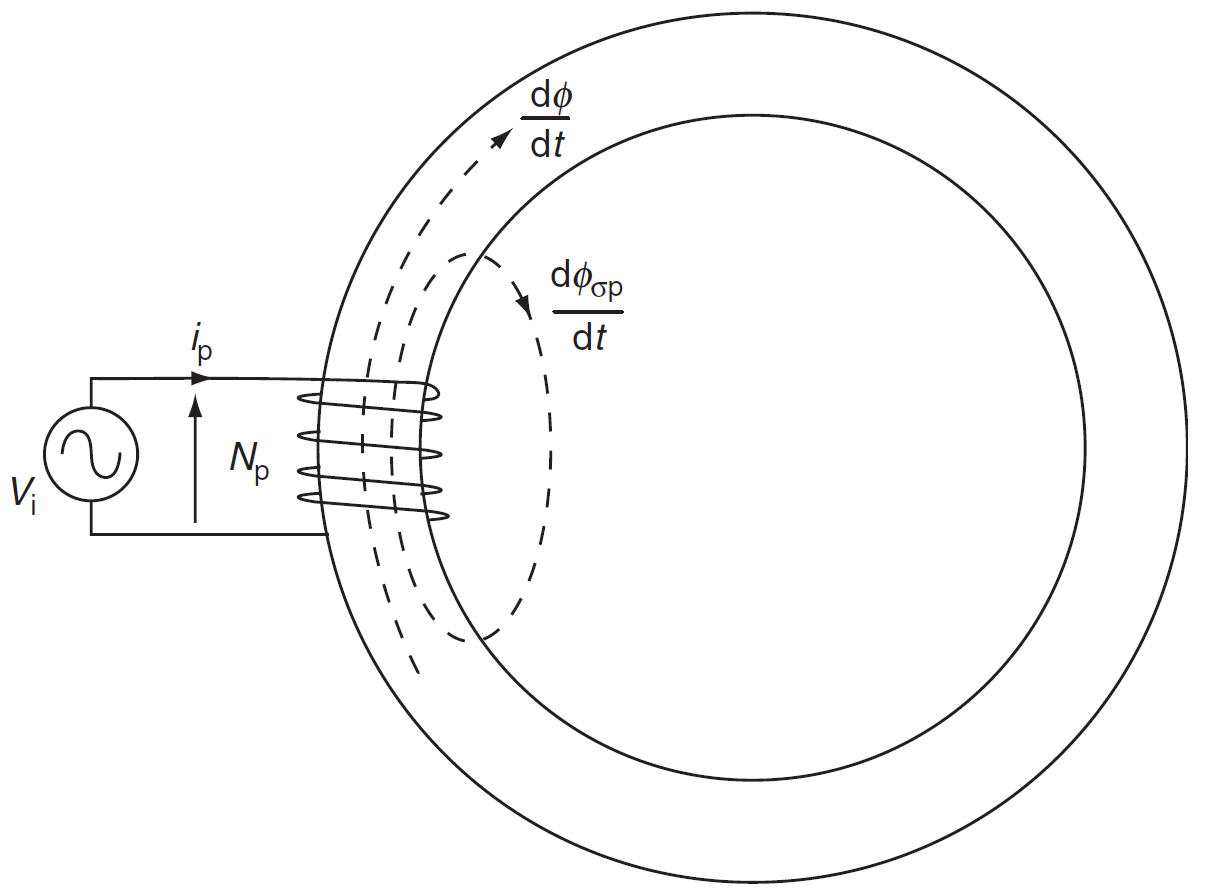
\includegraphics[width=\linewidth]{fig/lec07/linkage_flux.png}
                \caption{Leakage flux that does not fully link the second winding. Adapted from Umanand, \textit{Power Electronics: Essentials and Applications}}
            \end{figure}
        \end{column}
    \end{columns}
\end{frame}


%%%%%%%%%%%%%%%%%%%%%%%%%%%%%%%%%%%%%%%%%%%%%%%%%%%%%%%%%%%%%
%% Comparison of magnetic components
%%%%%%%%%%%%%%%%%%%%%%%%%%%%%%%%%%%%%%%%%%%%%%%%%%%%%%%%%%%%%
\begin{frame}
    \frametitle{Comparison of Practical Magnetic Components}

    \scriptsize
    \begin{table}
        \centering
        \begin{tabular}{p{0.22\textwidth}p{0.15\textwidth}p{0.15\textwidth}p{0.13\textwidth}p{0.22\textwidth}}
            \hline
            \textbf{Component} & \textbf{Stores Energy} & \textbf{Transfers Energy} & \textbf{Air Gap} & \textbf{Typical Use}\\
            \hline
            Filter inductor & Yes & No & Usually yes & Buck, boost, PFC, DC filters\\
            AC inductor / reactor & Yes & No & Sometimes & Grid filters, motor drives, rectifiers\\
            Coupled inductor & Yes & Partly & Sometimes & Interleaved converters, ripple cancellation\\
            Flyback transformer & Yes & Sequentially & Yes & Isolated low/medium-power supplies\\
            HF transformer & Ideally no & Yes & Usually no & LLC, DAB, PSFB, isolated converters\\
            Current transformer & No & Signal energy only & No & Sensing and protection\\
            \hline
        \end{tabular}
    \end{table}
    \begin{block}{Message}
        \small
        The distinction between stored energy and transferred energy is the most important conceptual difference between inductors, flyback magnetic components, and true transformers.
    \end{block}
\end{frame}

%%%%%%%%%%%%%%%%%%%%%%%%%%%%%%%%%%%%%%%%%%%%%%%%%%%%%%%%%%%%%
%% Transformer design section
%%%%%%%%%%%%%%%%%%%%%%%%%%%%%%%%%%%%%%%%%%%%%%%%%%%%%%%%%%%%%
\begin{frame}
\begin{center}
  \textbf{\Huge{Transformer Design}}\\[0.4cm]
  \textbf{\Large{From Converter Specification to Magnetic Hardware}}
\end{center}
\end{frame}


%%%%%%%%%%%%%%%%%%%%%%%%%%%%%%%%%%%%%%%%%%%%%%%%%%%%%%%%%%%%%
%% Transformer design inputs
%%%%%%%%%%%%%%%%%%%%%%%%%%%%%%%%%%%%%%%%%%%%%%%%%%%%%%%%%%%%%
\begin{frame}
    \frametitle{Transformer Design Inputs}

    \begin{columns}
        \begin{column}{0.58\textwidth}
            Transformer design begins from the converter-level specification, not from the core catalogue.

            \vspace{0.15cm}

            The main electrical inputs are:
            \begin{itemize}
                \item Input-voltage range: $V_{\mathrm{in,min}}$ to $V_{\mathrm{in,max}}$
                \item Output voltage and power: $V_o$, $P_o$
                \item Switching frequency: $f_s$
                \item Topology: flyback, forward, LLC, PSFB, DAB, etc.
                \item Maximum duty ratio or phase-shift range
                \item Required isolation voltage
                \item Allowed temperature rise
            \end{itemize}

            \vspace{0.15cm}

            These specifications determine the required volt-seconds, turns ratio, core size, winding current, insulation system, and thermal design.
        \end{column}

        \begin{column}{0.38\textwidth}
            \begin{block}{Design Message}
                \small
                A transformer cannot be designed independently of the converter topology. The applied voltage waveform determines the flux swing, while the winding currents determine copper loss and heating.
            \end{block}
        \end{column}
    \end{columns}
\end{frame}


%%%%%%%%%%%%%%%%%%%%%%%%%%%%%%%%%%%%%%%%%%%%%%%%%%%%%%%%%%%%%
%% Transformer design workflow
%%%%%%%%%%%%%%%%%%%%%%%%%%%%%%%%%%%%%%%%%%%%%%%%%%%%%%%%%%%%%
\begin{frame}
    \frametitle{Transformer Design Workflow}

    \begin{center}
    \begin{circuitikz}[scale=0.78, transform shape]
        \tikzstyle{block} = [draw, rounded corners, align=center,
        minimum width=3.0cm, minimum height=0.85cm]

        \node[block] (spec) at (0,0) {Converter\\specification};
        \node[block] (wave) at (4,0) {Voltage/current\\waveforms};
        \node[block] (core) at (8,0) {Core material\\and geometry};

        \node[block] (turns) at (8,-2) {Turns ratio and\\primary turns};
        \node[block] (wind) at (4,-2) {Winding area,\\wire/PCB traces};
        \node[block] (loss) at (0,-2) {Core loss and\\copper loss};

        \node[block] (thermal) at (0,-4) {Thermal and\\insulation check};
        \node[block] (iterate) at (4,-4) {Iterate design};
        \node[block] (proto) at (8,-4) {Prototype and\\measure};

        \draw[->, thick] (spec) -- (wave);
        \draw[->, thick] (wave) -- (core);
        \draw[->, thick] (core) -- (turns);
        \draw[->, thick] (turns) -- (wind);
        \draw[->, thick] (wind) -- (loss);
        \draw[->, thick] (loss) -- (thermal);
        \draw[->, thick] (thermal) -- (iterate);
        \draw[->, thick] (iterate) -- (proto);
        \draw[->, thick, dashed] (iterate.north) .. controls (4,-1.0) and (6,-1.0) .. (core.south);
    \end{circuitikz}
    \end{center}

    \vspace{0.15cm}

    \begin{block}{Practical Interpretation}
        \small
        Transformer design is iterative because turns, flux density, copper area, leakage inductance, temperature rise, and insulation clearance are strongly coupled.
    \end{block}
\end{frame}


%%%%%%%%%%%%%%%%%%%%%%%%%%%%%%%%%%%%%%%%%%%%%%%%%%%%%%%%%%%%%
%% Volt-second constraint
%%%%%%%%%%%%%%%%%%%%%%%%%%%%%%%%%%%%%%%%%%%%%%%%%%%%%%%%%%%%%
\begin{frame}
    \frametitle{Volt-Second Constraint and Primary Turns}

    \begin{columns}
        \begin{column}{0.5\textwidth}
            The primary turns are selected so that the core flux density remains below the allowable limit. From Faraday's law,
            \begin{align}
                v_1(t) = N_1 A_c \frac{dB(t)}{dt}
            \end{align}
            \begin{align}
                \text{Therefore,} \quad
                \Delta B =
                \frac{1}{N_1 A_c}
                \int_{t_1}^{t_2} v_1(t)\,dt
                =
                \frac{\lambda_1}{N_1 A_c}
            \end{align}

            Rearranging gives the minimum primary turns:
            \begin{align}
                N_1 \geq
                \frac{\lambda_1}{A_c \Delta B_{\max}}
            \end{align}
        \end{column}

        \begin{column}{0.48\textwidth}
            \begin{figure}
                \centering
                \includegraphics[width=0.75\linewidth]{fig/lec07/volt_sec.png}
                \caption{$\lambda_1$ is the applied positive volt-second on the primary winding. Primary voltage waveform and applied volt-seconds $\lambda_1$ used for transformer design. Adapted from Erickson and Maksimovi\'c, \textit{Fundamentals of Power Electronics}, 3rd edition}
            \end{figure}
        \end{column}
    \end{columns}
\end{frame}


%%%%%%%%%%%%%%%%%%%%%%%%%%%%%%%%%%%%%%%%%%%%%%%%%%%%%%%%%%%%%
%% Transformer saturation
%%%%%%%%%%%%%%%%%%%%%%%%%%%%%%%%%%%%%%%%%%%%%%%%%%%%%%%%%%%%%
\begin{frame}
    \frametitle{Transformer Saturation is a Volt-Second Problem}

    \begin{columns}
        \begin{column}{0.58\textwidth}
            A transformer saturates when the applied volt-seconds force the core flux density beyond the saturation limit. The core flux density is
            \begin{align}
                B(t)=\frac{1}{N_1A_c}\int v_1(t)\,dt
            \end{align}
            Hence, transformer saturation is mainly controlled by:
            \begin{itemize}
                \item Primary voltage waveform
                \item Number of primary turns
                \item Core cross-sectional area
                \item Reset condition or volt-second balance
            \end{itemize}
            Large load current does not automatically saturate a true transformer if the primary and secondary ampere-turns cancel properly.
        \end{column}

        \begin{column}{0.38\textwidth}
            \begin{block}{Important Correction}
                \small
                Adding an air gap does not solve saturation in a conventional transformer. It mainly lowers magnetizing inductance and increases magnetizing current.
            \end{block}

            \vspace{0.15cm}

            \begin{block}{Correct Remedies}
                \small
                Increase $N_1$, increase $A_c$, reduce volt-seconds, or ensure proper core reset.
            \end{block}
        \end{column}
    \end{columns}
\end{frame}


%%%%%%%%%%%%%%%%%%%%%%%%%%%%%%%%%%%%%%%%%%%%%%%%%%%%%%%%%%%%%
%% Core geometry and material selection
%%%%%%%%%%%%%%%%%%%%%%%%%%%%%%%%%%%%%%%%%%%%%%%%%%%%%%%%%%%%%
\begin{frame}
    \frametitle{Core Geometry and Material Selection}
            Core selection determines the magnetic, electrical, thermal, and manufacturing limits of the transformer.

            \vspace{0.15cm}

            Important core parameters are:
            \begin{itemize}
                \item Effective core area $A_c$ or $A_e$
                \item Window area $A_w$ or $W_A$
                \item Magnetic path length $l_m$
                \item Mean length per turn MLT
                \item Core volume $V_c$
                \item Core material and loss data
            \end{itemize}
            Typical high-frequency core families include EE, EI, ER, ETD, PQ, RM and low-profile planar variants.
\end{frame}


\begin{frame}
    \frametitle{Core Geometry and Material Selection}
    \begin{columns}
        \begin{column}{0.5\textwidth}
            \begin{figure}
                \centering
                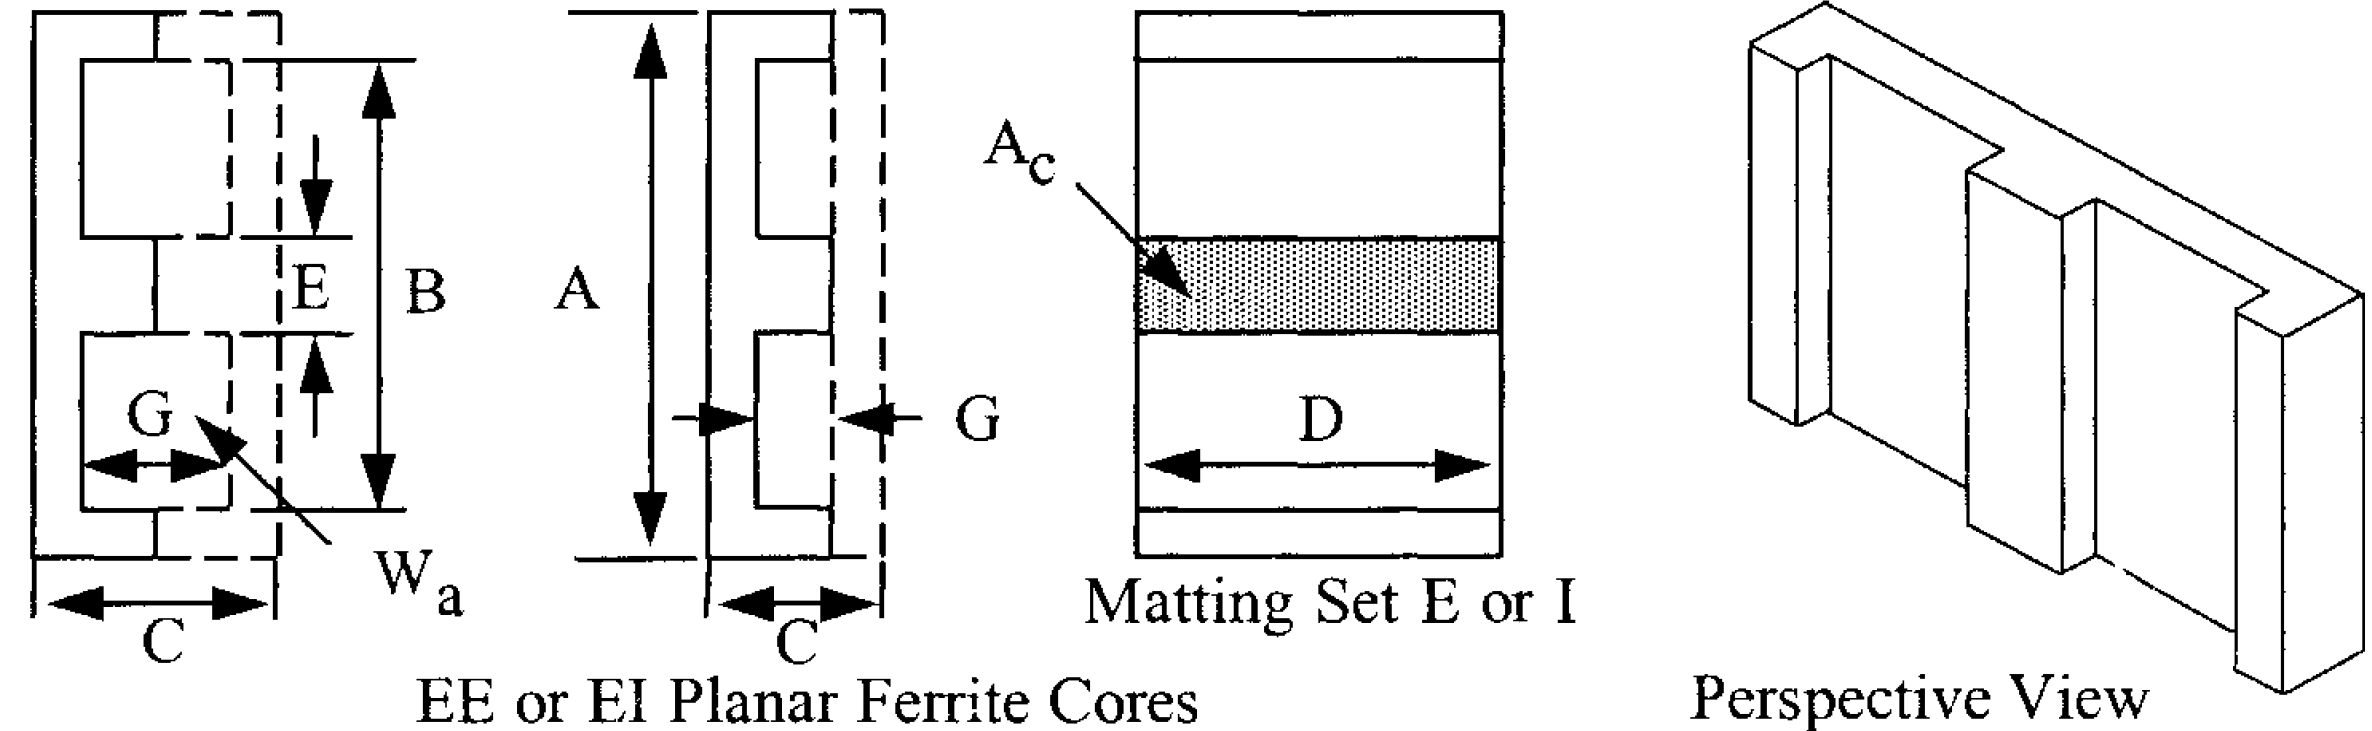
\includegraphics[width=0.75\linewidth]{fig/lec07/EE_core.png}
                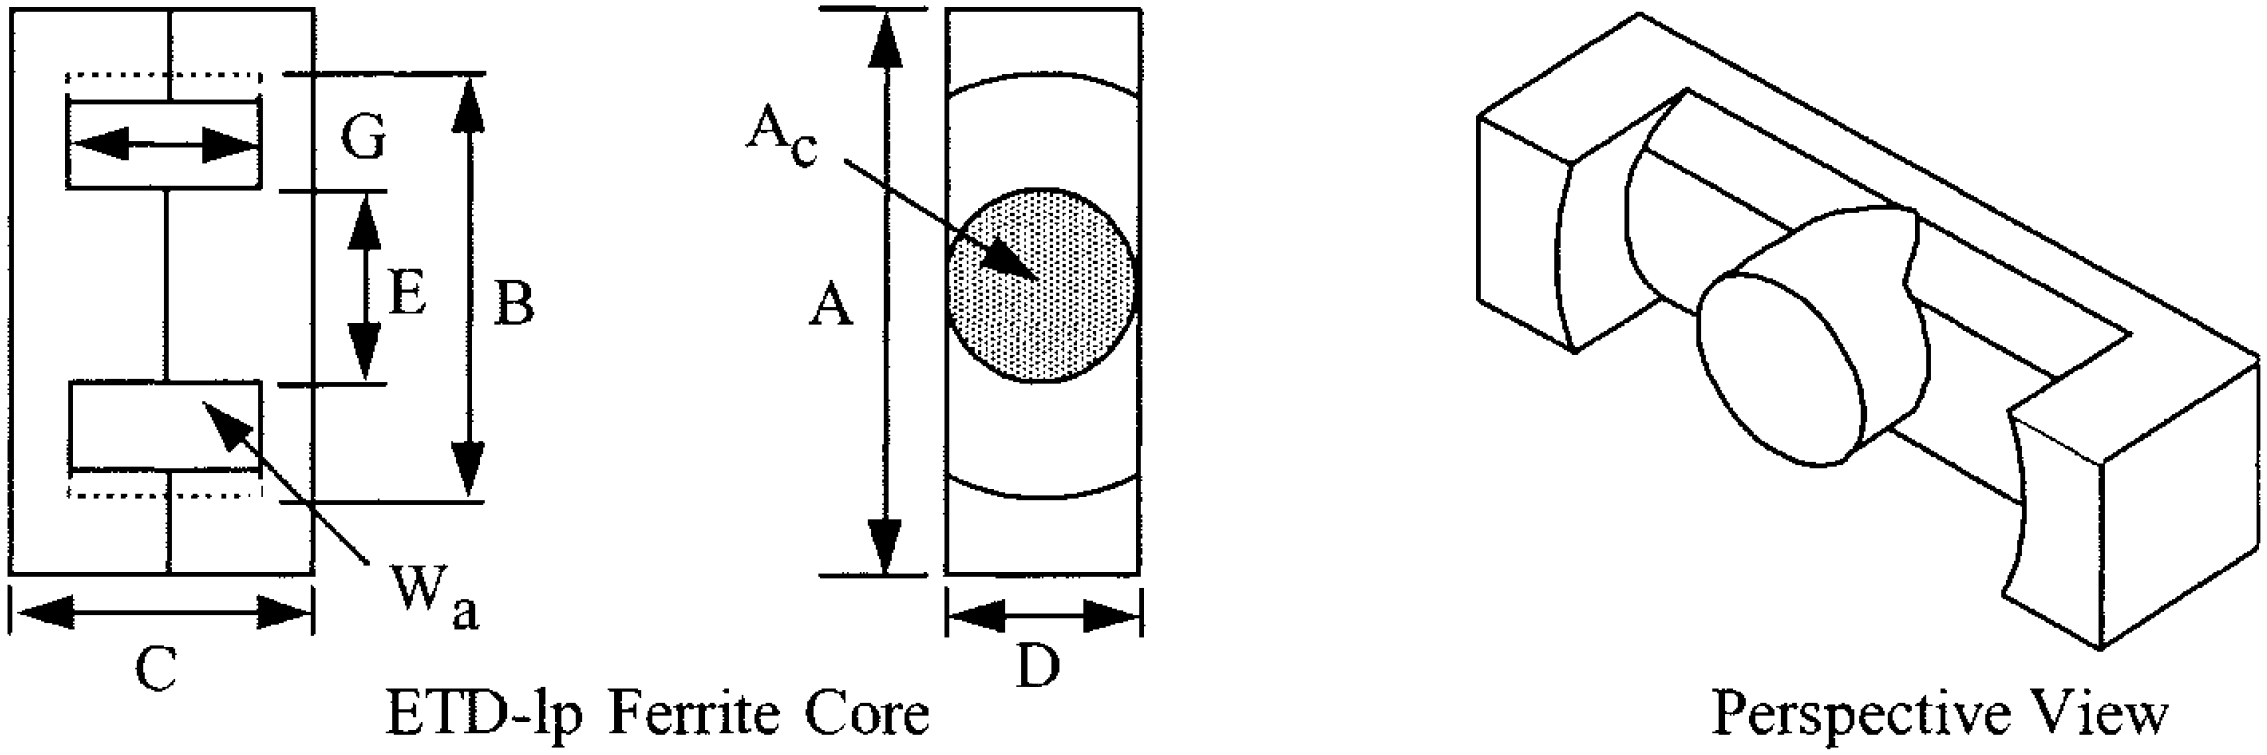
\includegraphics[width=0.75\linewidth]{fig/lec07/ETD_core.png}
              \caption{Low-profile planar core geometries including EE/EI, ER, ETD families. Adapted from \textit{Transformer and Inductor Design Handbook}}
            \end{figure}
        \end{column}

        \begin{column}{0.5\textwidth}
            \begin{figure}
                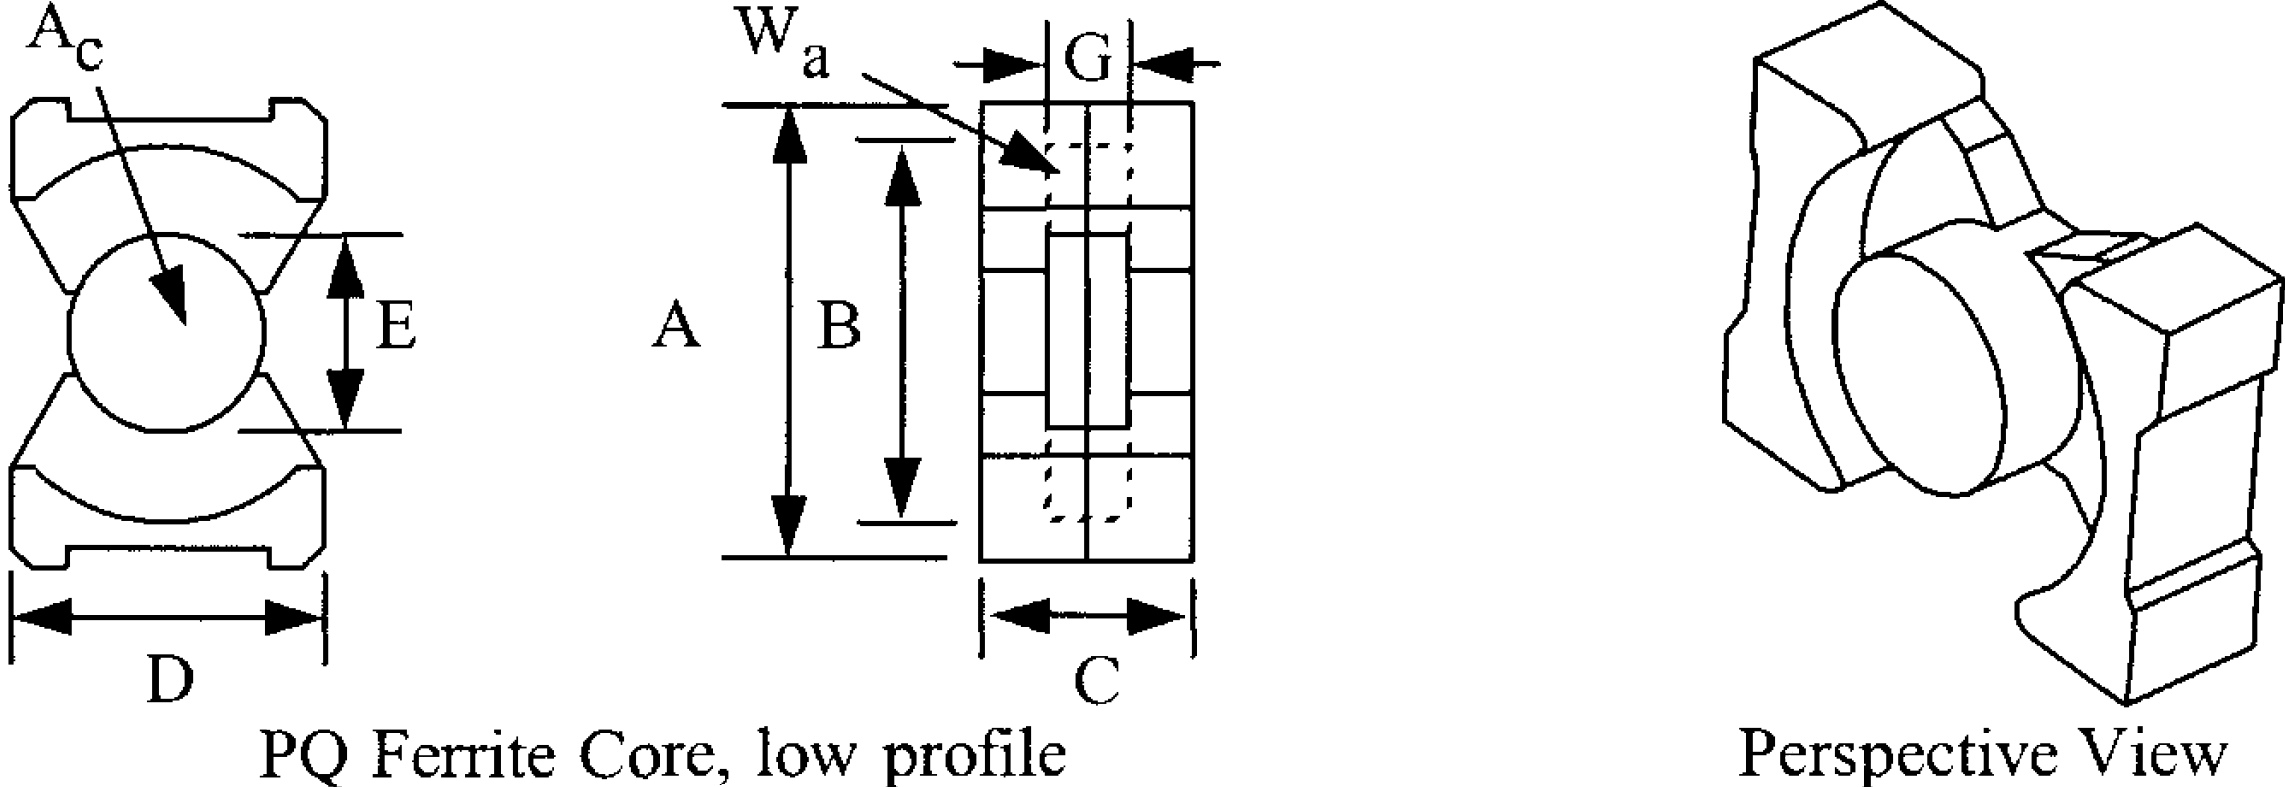
\includegraphics[width=0.75\linewidth]{fig/lec07/PQ_core.png}
                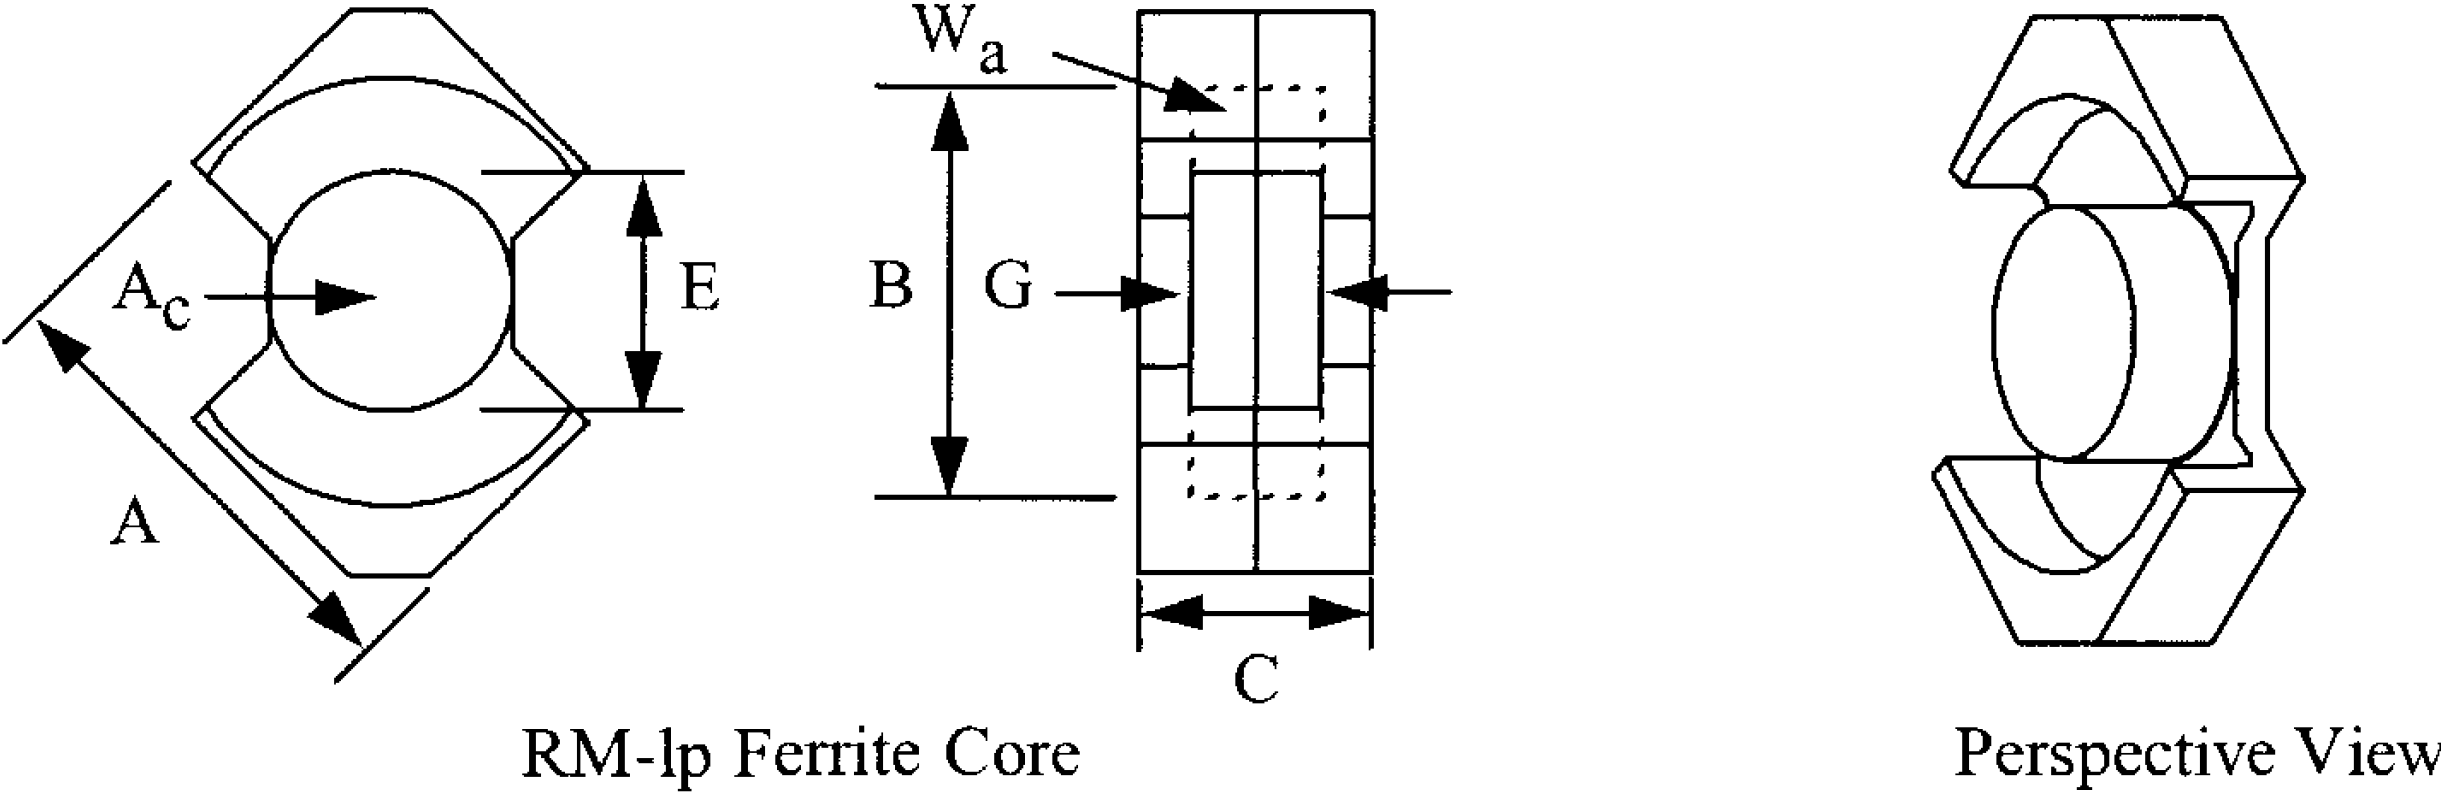
\includegraphics[width=0.5\linewidth]{fig/lec07/RM_core.png}
                \caption{Low-profile planar core geometries including PQ and RM families. Adapted from \textit{Transformer and Inductor Design Handbook}}
            \end{figure}
        \end{column}
    \end{columns}
\end{frame}
%%%%%%%%%%%%%%%%%%%%%%%%%%%%%%%%%%%%%%%%%%%%%%%%%%%%%%%%%%%%%
%% Area product and core size
%%%%%%%%%%%%%%%%%%%%%%%%%%%%%%%%%%%%%%%%%%%%%%%%%%%%%%%%%%%%%
\begin{frame}
    \frametitle{Area Product and Core-Size Selection}

    \begin{columns}
        \begin{column}{0.58\textwidth}
            The core must simultaneously satisfy magnetic and winding-space constraints. The area product is
            \begin{align}
                A_P = A_c A_w
            \end{align}

            where
            \begin{itemize}
                \item $A_c$ supports the required flux,
                \item $A_w$ provides space for the windings.
            \end{itemize}
            For transformer designs where core loss is important, a core geometrical constant $K_{gfe}$ is introduced as a first-pass sizing parameter:
            \begin{align}
                K_{gfe} \geq K_{gfe,\mathrm{req}}
            \end{align}
        \end{column}

        \begin{column}{0.38\textwidth}
            This approach using $K_{gfe}$ accounts for both copper loss and core loss in selecting a suitable core size.
            \begin{block}{Design Interpretation}
                \small
                At high frequency, transformer design is often not saturation-limited. It is frequently core-loss-limited, so the selected $\Delta B$ is much lower than $B_{\mathrm{sat}}$.
            \end{block}
        \end{column}
    \end{columns}
\end{frame}


%%%%%%%%%%%%%%%%%%%%%%%%%%%%%%%%%%%%%%%%%%%%%%%%%%%%%%%%%%%%%
%% Turns ratio and secondary turns
%%%%%%%%%%%%%%%%%%%%%%%%%%%%%%%%%%%%%%%%%%%%%%%%%%%%%%%%%%%%%
\begin{frame}
    \frametitle{Turns Ratio and Secondary Turns}

    \begin{columns}
        \begin{column}{0.58\textwidth}
            The turns ratio is selected from converter voltage gain and device-voltage stress requirements. For an ideal transformer,
            \begin{align}
                \frac{v_2}{v_1}=\frac{N_2}{N_1}=n
            \end{align}
            Once $N_1$ is selected from the volt-second constraint, the secondary turns are $N_2 = nN_1$.
            In practical design:
            \begin{itemize}
                \item $N_1$ and $N_2$ must be rounded to integers.
                \item Rounding changes the actual turns ratio.
                \item The new ratio must be checked against voltage gain and semiconductor stress.
                \item Multi-output transformers require additional secondary turns and regulation checks.
            \end{itemize}
        \end{column}

        \begin{column}{0.38\textwidth}
            \begin{figure}
                \centering
                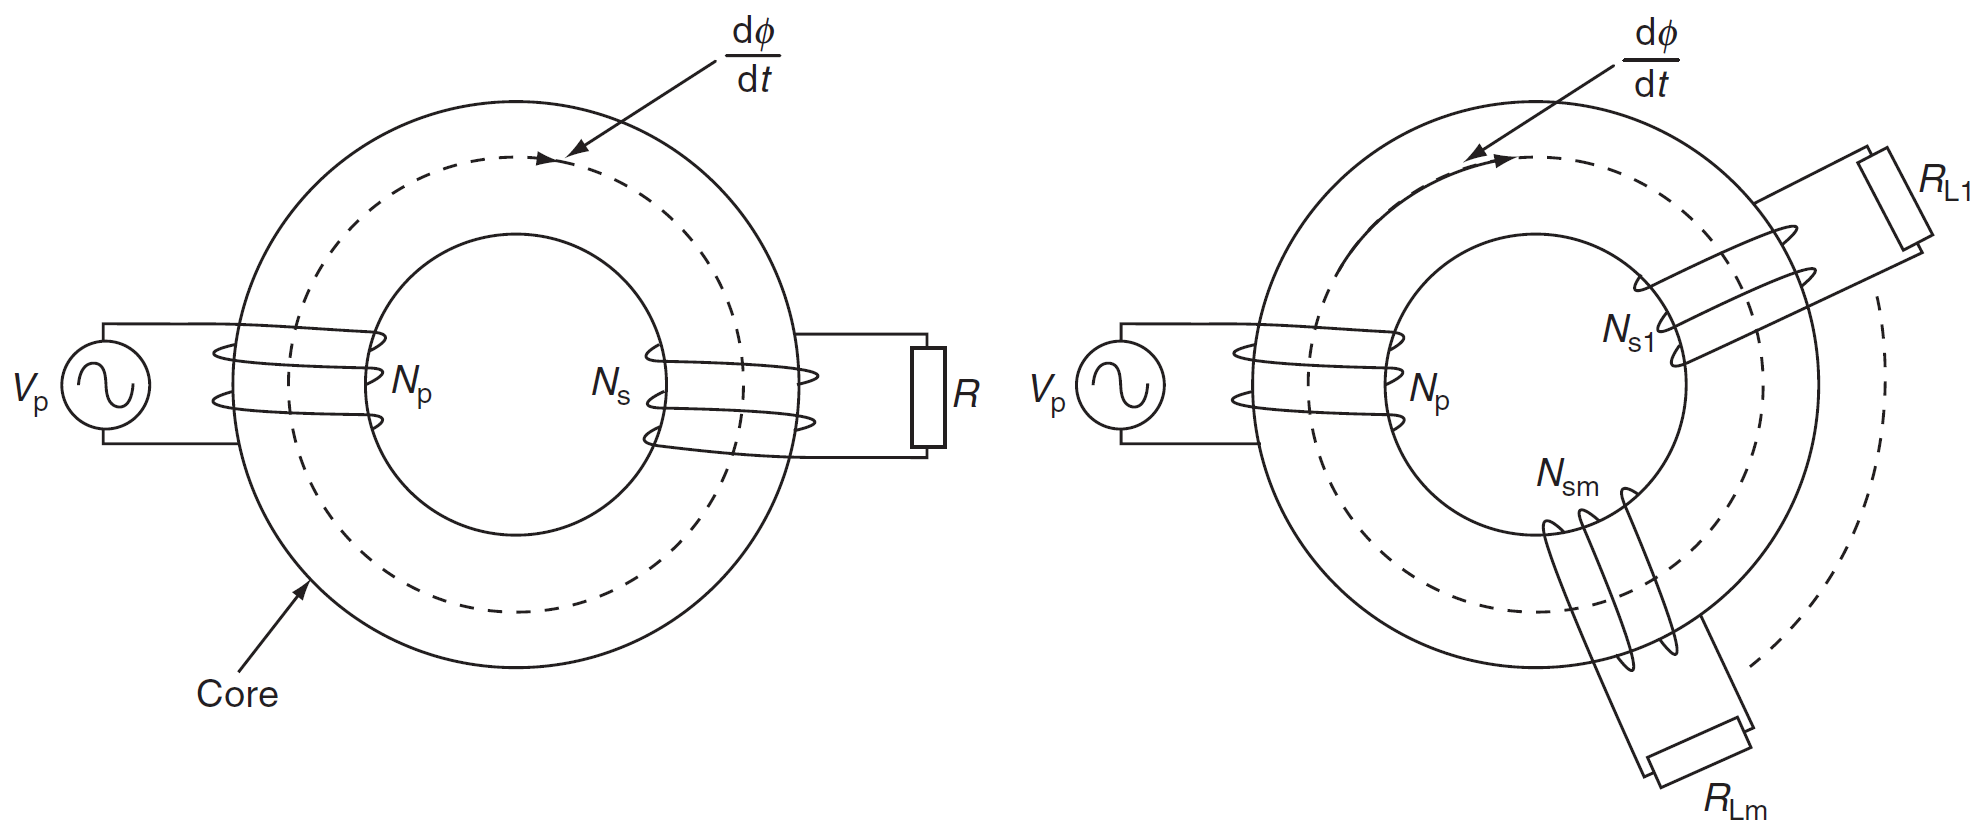
\includegraphics[width=\linewidth]{fig/lec07/trans_sec_winding.png}
                \caption{Single-secondary and multiple-secondary transformer structures. Adapted from Umanand, \textit{Power Electronics: Essentials and Applications}}
            \end{figure}
        \end{column}
    \end{columns}
\end{frame}


%%%%%%%%%%%%%%%%%%%%%%%%%%%%%%%%%%%%%%%%%%%%%%%%%%%%%%%%%%%%%
%% Winding area and current density
%%%%%%%%%%%%%%%%%%%%%%%%%%%%%%%%%%%%%%%%%%%%%%%%%%%%%%%%%%%%%
\begin{frame}
    \frametitle{Winding Area, Fill Factor, and Current Density}

    \begin{columns}
        \begin{column}{0.58\textwidth}
            After determining the turns, the winding must physically fit inside the available window area. The available copper area is $
                A_{\mathrm{Cu,available}} = K_u W_A$, 
            where $K_u$ is the window utilization or fill factor. For each winding,
            \begin{align}
                A_{w,j} \approx \frac{I_{j,\mathrm{rms}}}{J}
            \end{align}
            where $J$ is the allowable current density. The selected winding must satisfy:
            \begin{itemize}
                \item DC resistance limit
                \item AC resistance limit
                \item Temperature-rise limit
                \item Insulation and creepage/clearance limits
            \end{itemize}
        \end{column}

        \begin{column}{0.38\textwidth}
            \begin{figure}
                \centering
                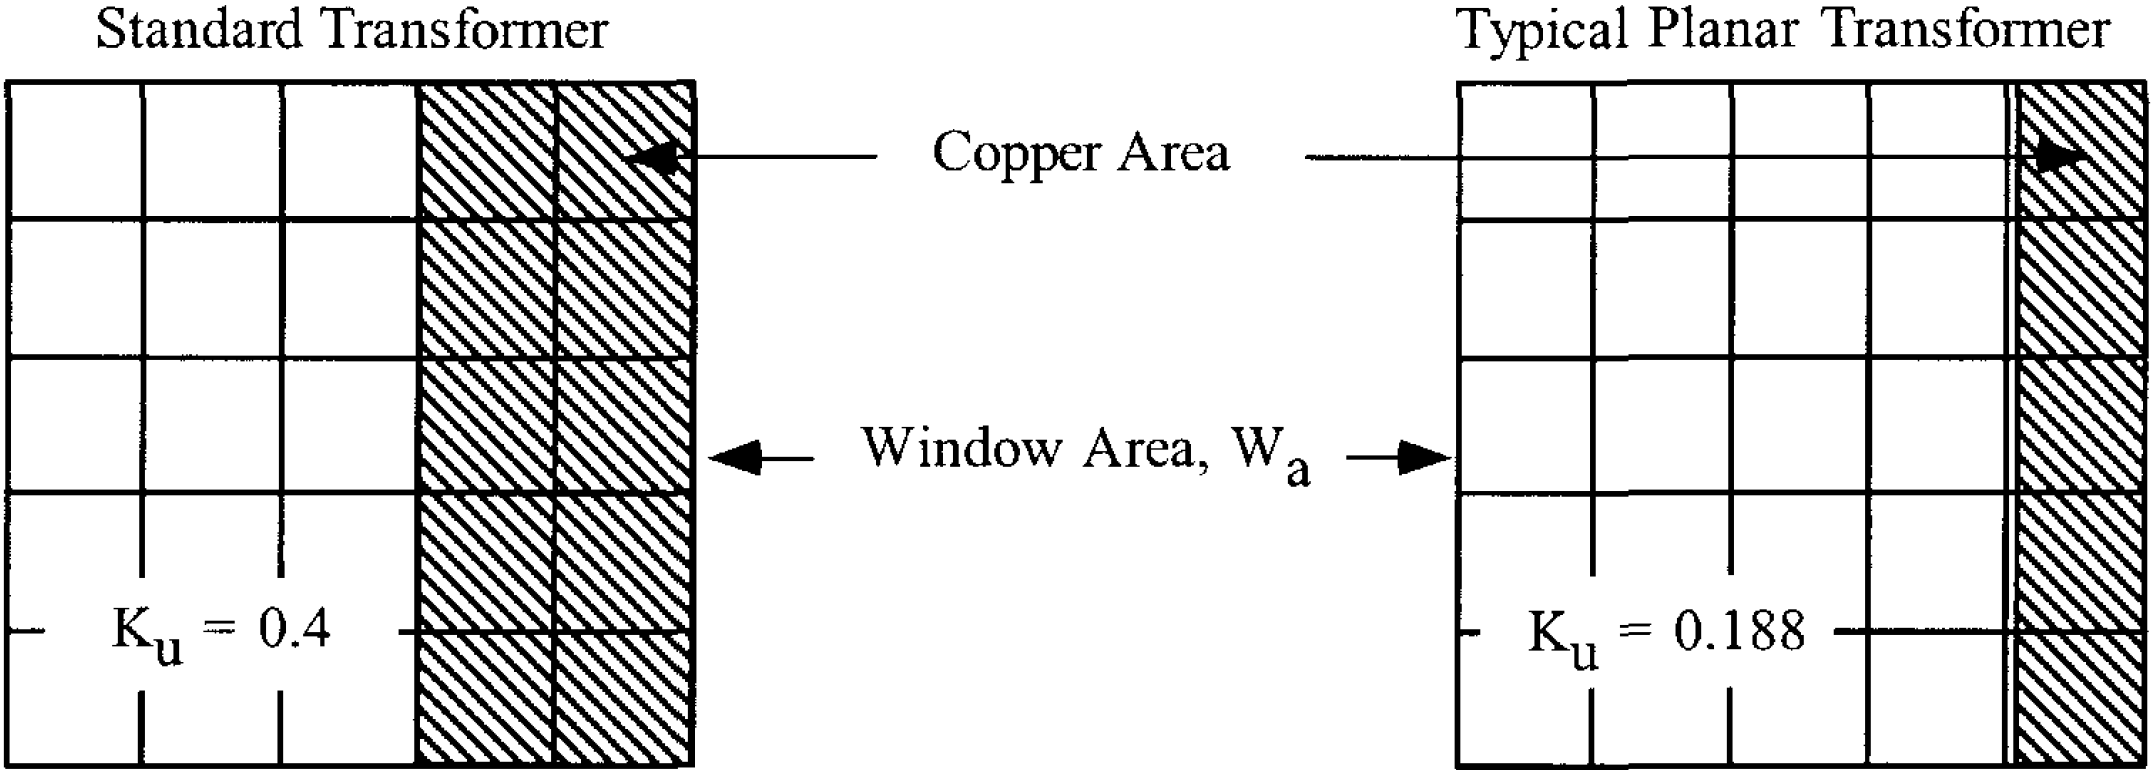
\includegraphics[width=\linewidth]{fig/lec07/window_uti.png}
                \caption{Comparison of window utilization in standard and planar transformers. Adapted from \textit{Transformer and Inductor Design Handbook}}
            \end{figure}
        \end{column}
    \end{columns}
\end{frame}


%%%%%%%%%%%%%%%%%%%%%%%%%%%%%%%%%%%%%%%%%%%%%%%%%%%%%%%%%%%%%
%% Planar transformer winding design
%%%%%%%%%%%%%%%%%%%%%%%%%%%%%%%%%%%%%%%%%%%%%%%%%%%%%%%%%%%%%
\begin{frame}
    \frametitle{Planar Transformer Winding Design}

    \begin{columns}
        \begin{column}{0.58\textwidth}
            In planar transformers, the winding is implemented using PCB copper, flexible PCB, stamped copper, or a hybrid structure.

            \vspace{0.15cm}

            The main winding decisions are:
            \begin{itemize}
                \item Copper thickness: 1 oz, 2 oz, 3 oz, or thicker copper
                \item Track width and spacing
                \item Number of PCB layers
                \item Via current capability
                \item Layer-to-layer insulation
                \item Primary-secondary arrangement
            \end{itemize}

            \vspace{0.15cm}

            Planar windings provide excellent repeatability and controlled parasitics, but they can suffer from low window utilization and high interwinding capacitance.
        \end{column}

        \begin{column}{0.38\textwidth}
            \begin{figure}
                \centering
                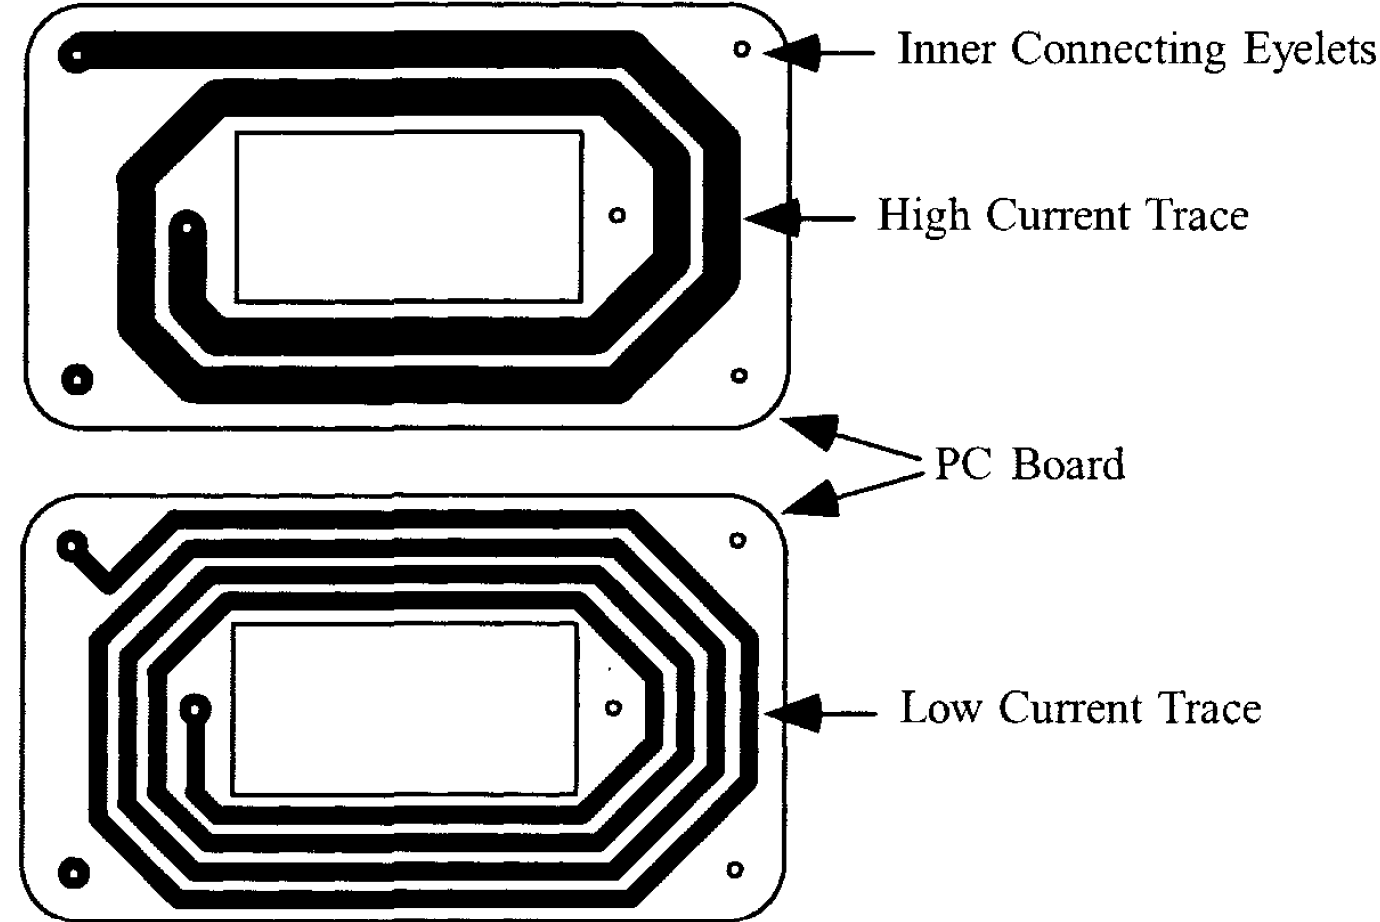
\includegraphics[width=\linewidth]{fig/lec07/planer_E_core_winding.png}
                \caption{Typical planar E-core winding PCB with high-current and low-current traces. Adapted from \textit{Transformer and Inductor Design Handbook}}
            \end{figure}
        \end{column}
    \end{columns}
\end{frame}


%%%%%%%%%%%%%%%%%%%%%%%%%%%%%%%%%%%%%%%%%%%%%%%%%%%%%%%%%%%%%
%% Leakage and magnetizing inductance check
%%%%%%%%%%%%%%%%%%%%%%%%%%%%%%%%%%%%%%%%%%%%%%%%%%%%%%%%%%%%%
\begin{frame}
    \frametitle{Magnetizing and Leakage Inductance Check}

    \begin{columns}
        \begin{column}{0.58\textwidth}
            After the first-pass design, the transformer must be checked using its equivalent circuit. The magnetizing inductance is approximately $L_M = \frac{N_1^2}{\mathcal{R}}$, and determines the magnetizing current:
            \begin{align}
                i_M(t)=\frac{1}{L_M}\int v_1(t)\,dt
            \end{align}
            Leakage inductance appears in series with the windings and affects:
            \begin{itemize}
                \item Voltage spikes
                \item Current transfer
                \item Ringing frequency
                \item Resonant-tank behaviour
                \item Snubber or clamp design
            \end{itemize}
        \end{column}

        \begin{column}{0.38\textwidth}
            \begin{figure}
                \centering
                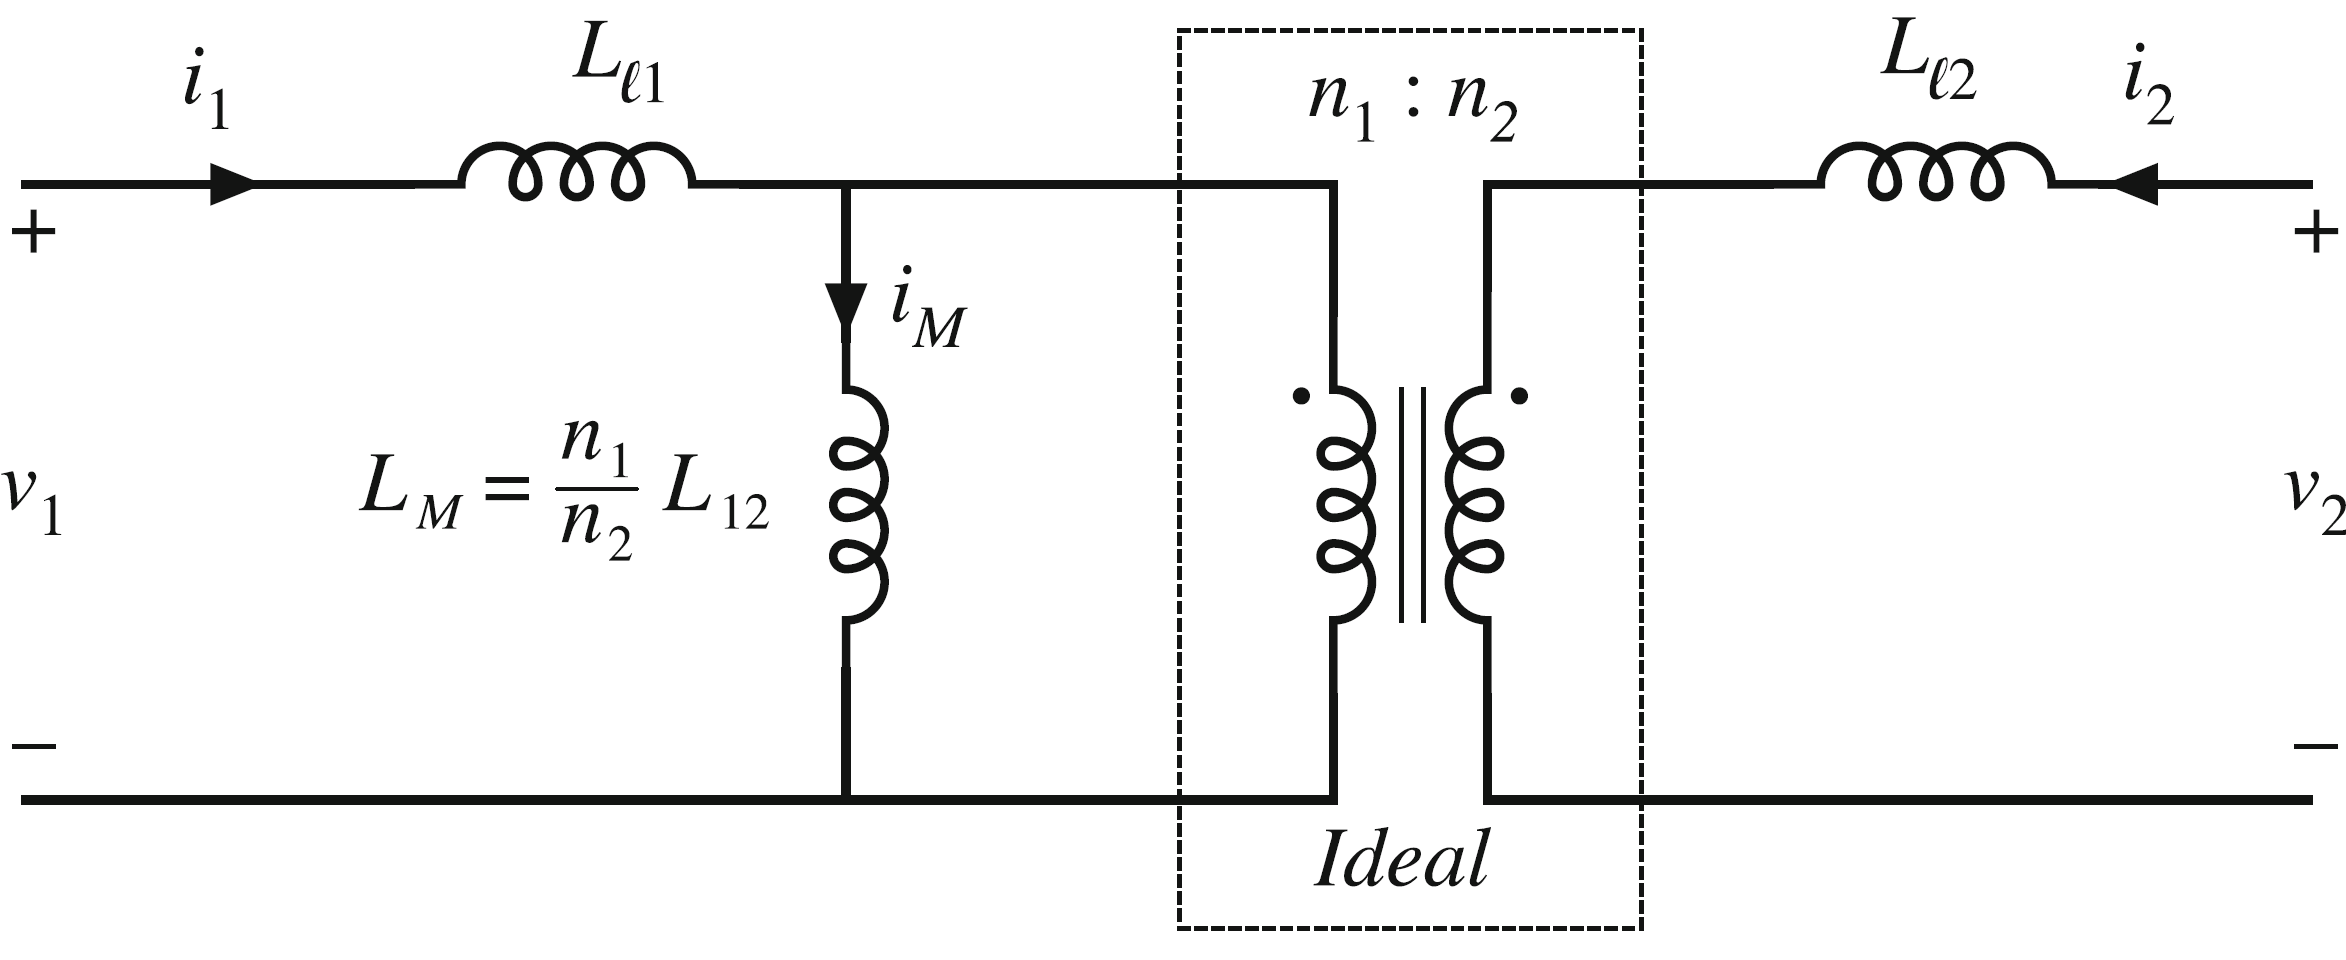
\includegraphics[width=\linewidth]{fig/lec07/transformer_equivalent_circuit.png}
                \caption{Two-winding transformer equivalent circuit including magnetizing inductance and primary/secondary leakage inductances. Adapted from Erickson and Maksimovi\'c, \textit{Fundamentals of Power Electronics}, 3rd edition}
            \end{figure}
        \end{column}
    \end{columns}
\end{frame}


%%%%%%%%%%%%%%%%%%%%%%%%%%%%%%%%%%%%%%%%%%%%%%%%%%%%%%%%%%%%%
%% Design verification and iteration
%%%%%%%%%%%%%%%%%%%%%%%%%%%%%%%%%%%%%%%%%%%%%%%%%%%%%%%%%%%%%
\begin{frame}
    \frametitle{Transformer Design Verification}

    \begin{columns}
        \begin{column}{0.58\textwidth}
            A transformer design is acceptable only after electrical, magnetic, thermal, and insulation checks are satisfied.

            \vspace{0.15cm}

            Minimum verification checklist:
            \begin{itemize}
                \item Flux density:
                \[
                    \Delta B < \Delta B_{\max}
                \]
                \item Core loss from material loss curves or Steinmetz model
                \item DC and AC copper losses
                \item Leakage inductance and parasitic capacitance
                \item Temperature rise at worst-case operation
                \item Isolation, creepage and clearance
                \item Manufacturability and repeatability
            \end{itemize}

        \end{column}

        \begin{column}{0.38\textwidth}
        High-frequency transformers usually require several design iterations.
            \begin{block}{First-Pass Design is Not Final}
                \small
                Analytical equations select a candidate core and turns. Final design requires loss estimation, thermal validation, parasitic extraction, and experimental measurement.
            \end{block}
        \end{column}
    \end{columns}
\end{frame}

%%%%%%%%%%%%%%%%%%%%%%%%%%%%%%%%%%%%%%%%%%%%%%%%%%%%%%%%%%%%%
%% Module 3
%%%%%%%%%%%%%%%%%%%%%%%%%%%%%%%%%%%%%%%%%%%%%%%%%%%%%%%%%%%%%
\begin{frame}
\begin{center}
  \textbf{\Huge{Winding Arrangements}}\\[0.4cm]
  \textbf{\Large{Leakage, AC Resistance, Capacitance, and Manufacturability}}
\end{center}
\end{frame}


%%%%%%%%%%%%%%%%%%%%%%%%%%%%%%%%%%%%%%%%%%%%%%%%%%%%%%%%%%%%%
%% Why winding arrangement matters
%%%%%%%%%%%%%%%%%%%%%%%%%%%%%%%%%%%%%%%%%%%%%%%%%%%%%%%%%%%%%
\begin{frame}
    \frametitle{Why Winding Arrangement Matters}

    \begin{columns}
        \begin{column}{0.58\textwidth}
            In high-frequency magnetic components, the winding arrangement is often as important as the core material. It directly influences:
            \begin{itemize}
                \item Leakage inductance
                \item Proximity-effect loss
                \item Skin-effect loss
                \item Interwinding capacitance
                \item Common-mode noise
                \item Thermal path from copper to ambient
                \item Manufacturability and repeatability
            \end{itemize}
            In low-frequency transformers, winding design is mainly about copper area and insulation. In high-frequency power electronics, it is also about controlling the magnetic field distribution inside the winding window.
        \end{column}

        \begin{column}{0.38\textwidth}
            \begin{block}{Design Message}
                \small
                A transformer with the correct turns ratio can still perform poorly if the winding layout produces excessive leakage inductance, AC resistance, or parasitic capacitance.
            \end{block}
        \end{column}
    \end{columns}
\end{frame}


%%%%%%%%%%%%%%%%%%%%%%%%%%%%%%%%%%%%%%%%%%%%%%%%%%%%%%%%%%%%%
%% Layered winding
%%%%%%%%%%%%%%%%%%%%%%%%%%%%%%%%%%%%%%%%%%%%%%%%%%%%%%%%%%%%%
\begin{frame}
    \frametitle{Layered Winding}

    \begin{columns}
        \begin{column}{0.58\textwidth}
            A layered winding places one winding layer after another inside the core window. This is simple and manufacturable, but it may produce high leakage inductance and high proximity loss. Typical structure:
            \begin{itemize}
                \item Primary layers grouped together
                \item Secondary layers grouped together
                \item Insulation placed between primary and secondary
            \end{itemize}

        \end{column}

        \begin{column}{0.38\textwidth}
            \begin{figure}
                \centering
                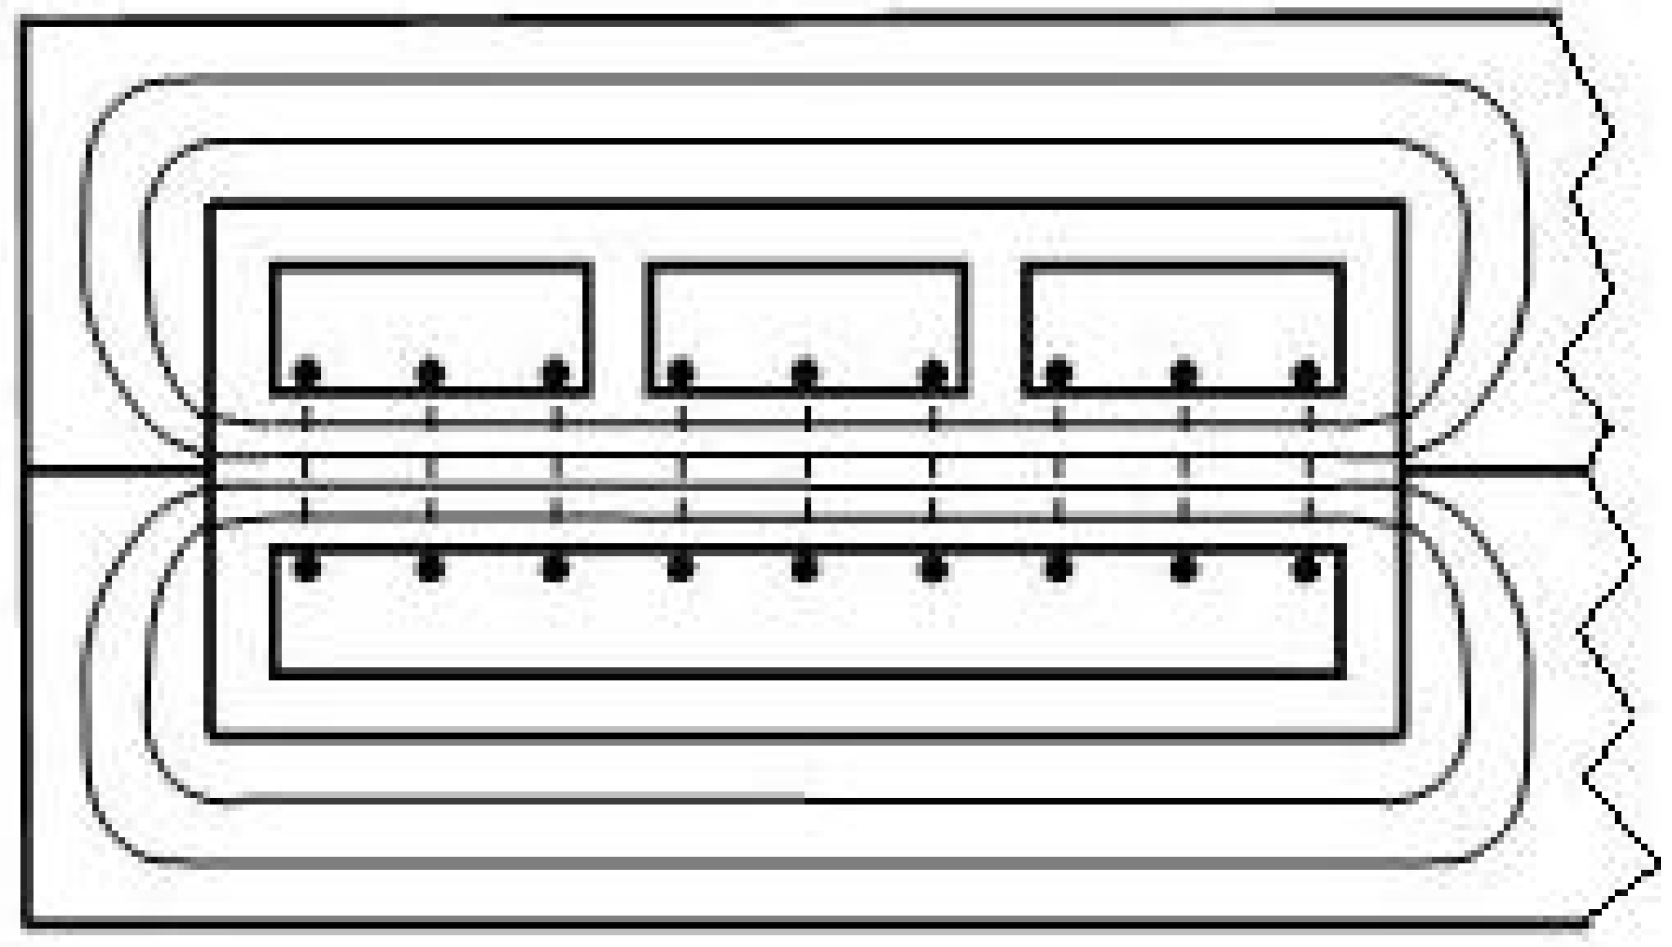
\includegraphics[width=\linewidth]{fig/lec07/planar_transformer_flux.png}
                \caption{Magnetic force equipotentials and leakage flux lines between primary and secondary windings in a planar transformer. Adapted from Dixon, Texas Instruments, \textit{Designing Planar Magnetics}}
            \end{figure}
        \end{column}
    \end{columns}
\end{frame}

%%%%%%%%%%%%%%%%%%%%%%%%%%%%%%%%%%%%%%%%%%%%%%%%%%%%%%%%%%%%%
%% Layered winding
%%%%%%%%%%%%%%%%%%%%%%%%%%%%%%%%%%%%%%%%%%%%%%%%%%%%%%%%%%%%%
\begin{frame}
    \frametitle{Layered Winding}

    \begin{columns}
        \begin{column}{0.58\textwidth}
            Advantages:
            \begin{itemize}
                \item Simple construction
                \item Good insulation control
                \item Easy to manufacture
            \end{itemize}

            Limitations:
            \begin{itemize}
                \item Larger leakage field between winding groups
                \item Increased AC winding resistance
                \item Poorer transient behaviour in hard-switched converters
            \end{itemize}
        \end{column}

        \begin{column}{0.38\textwidth}
            \begin{figure}
                \centering
                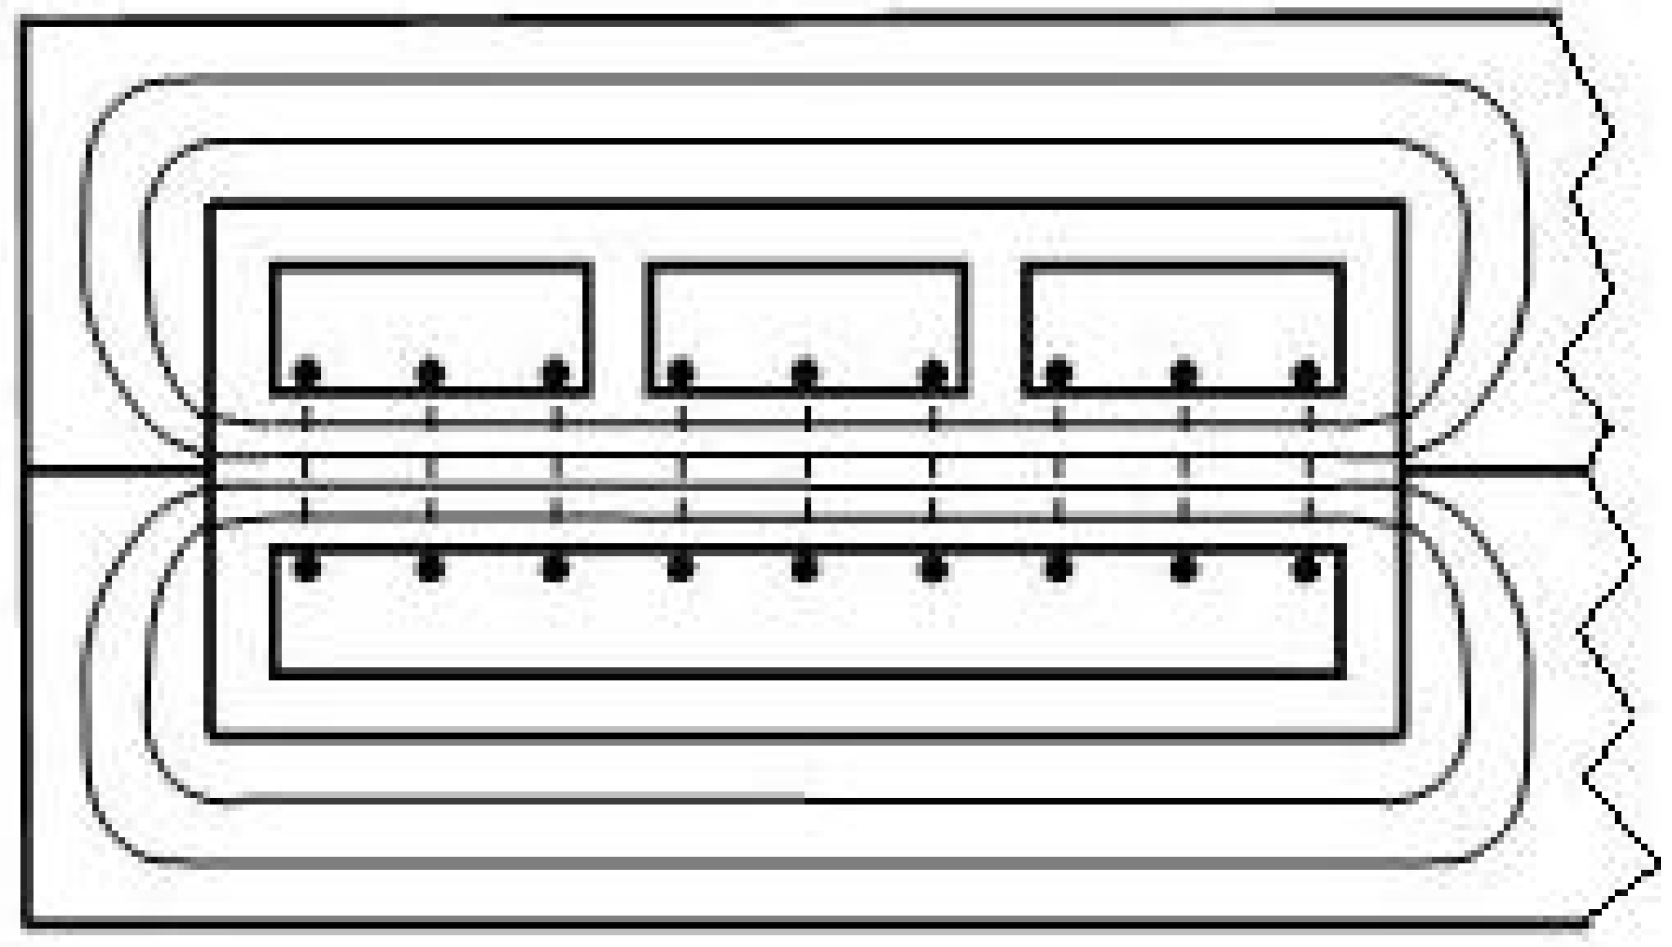
\includegraphics[width=\linewidth]{fig/lec07/planar_transformer_flux.png}
                \caption{Magnetic force equipotentials and leakage flux lines between primary and secondary windings in a planar transformer. Adapted from Dixon, Texas Instruments, \textit{Designing Planar Magnetics}}
            \end{figure}
        \end{column}
    \end{columns}
\end{frame}

%%%%%%%%%%%%%%%%%%%%%%%%%%%%%%%%%%%%%%%%%%%%%%%%%%%%%%%%%%%%%
%% Sectional winding
%%%%%%%%%%%%%%%%%%%%%%%%%%%%%%%%%%%%%%%%%%%%%%%%%%%%%%%%%%%%%
\begin{frame}
    \frametitle{Sectional Winding}

    \begin{columns}
        \begin{column}{0.58\textwidth}
            In sectional winding, the winding is divided into sections rather than being placed as one continuous block. The purpose is to control the spatial distribution of magnetic field and electric field inside the winding window.
            Sectional winding can be useful when:
            \begin{itemize}
                \item High isolation voltage is required
                \item Interwinding capacitance must be reduced
                \item Leakage inductance must be intentionally adjusted
                \item Multiple outputs require physical separation
            \end{itemize}

            Compared with full interleaving, sectional winding may increase leakage inductance, but can reduce capacitance and simplify insulation design.
        \end{column}

        \begin{column}{0.38\textwidth}
            \begin{block}{Engineering Trade-off}
                \small
                Interleaving generally reduces leakage inductance but increases capacitance.

                \vspace{0.15cm}

                Sectionalization generally reduces capacitance and improves insulation control but can increase leakage inductance.
            \end{block}
        \end{column}
    \end{columns}
\end{frame}


%%%%%%%%%%%%%%%%%%%%%%%%%%%%%%%%%%%%%%%%%%%%%%%%%%%%%%%%%%%%%
%% Interleaved winding
%%%%%%%%%%%%%%%%%%%%%%%%%%%%%%%%%%%%%%%%%%%%%%%%%%%%%%%%%%%%%
\begin{frame}
    \frametitle{Interleaved Winding}

    \begin{columns}
        \begin{column}{0.55\textwidth}
            Interleaving alternates primary and secondary winding sections to reduce the magnetic field energy stored between them. Examples:
            \begin{itemize}
                \item P--S--P
                \item S--P--S
                \item P--S--P--S
                \item PCB layer interleaving in planar transformers
            \end{itemize}
            Main benefits:
            \begin{itemize}
                \item Reduced leakage inductance
                \item Reduced voltage overshoot
                \item Better current transfer
                \item Lower proximity-effect loss in many transformer cases
            \end{itemize}
        \end{column}

        \begin{column}{0.44\textwidth}
            \begin{figure}
                \centering
                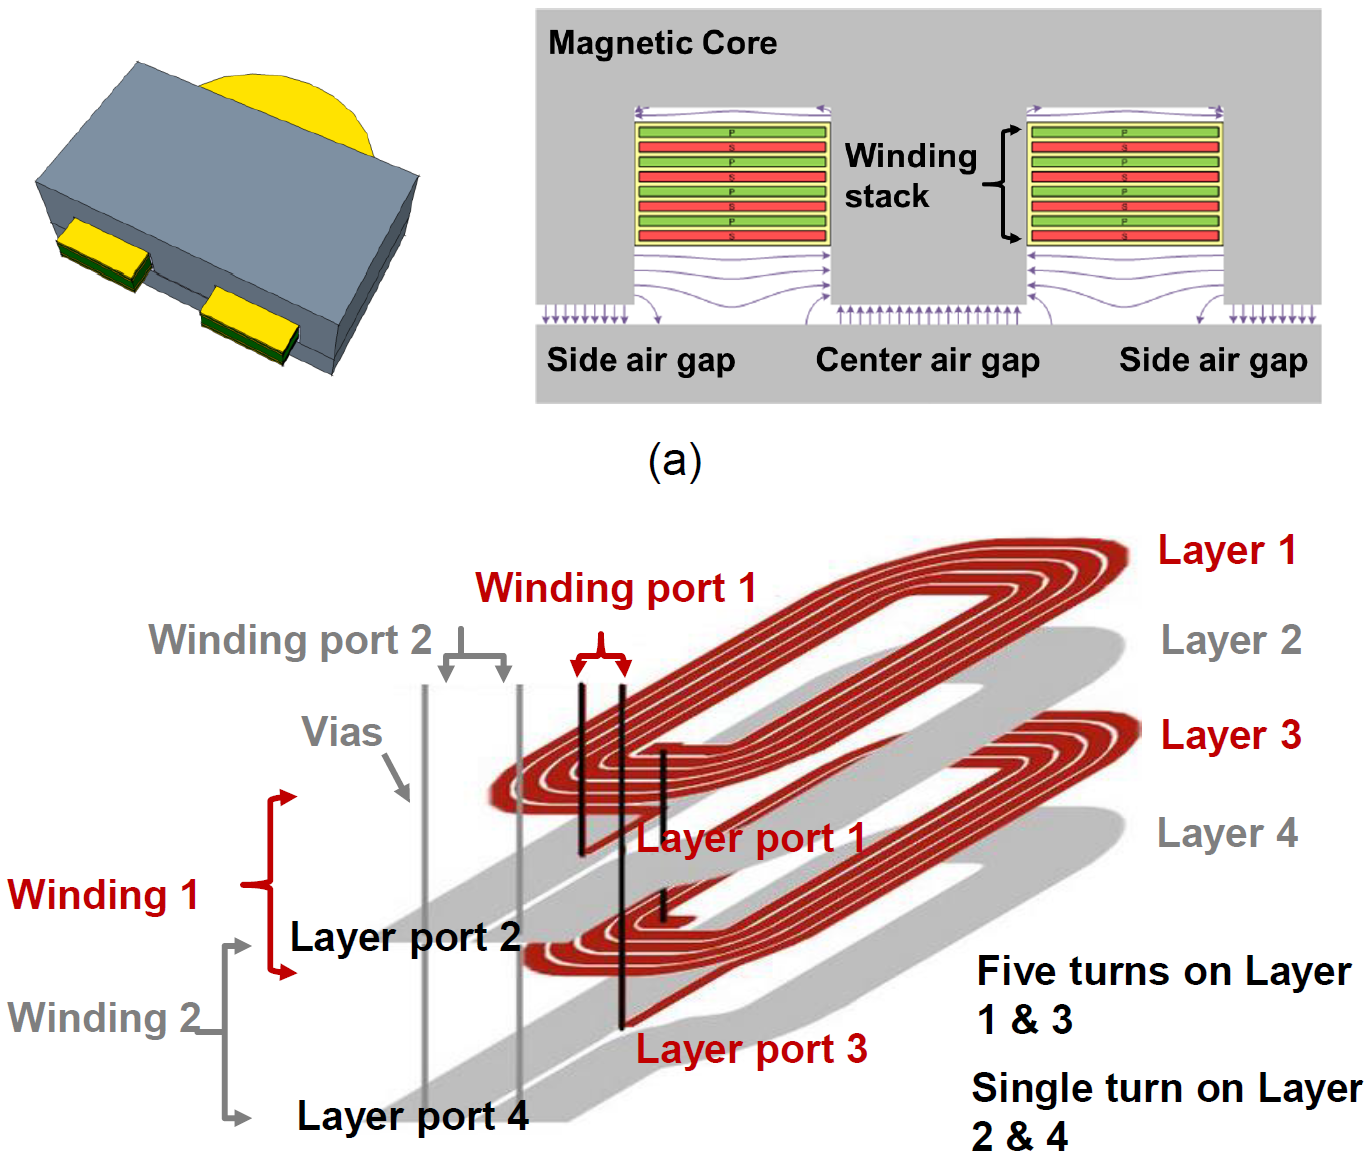
\includegraphics[width=0.8\linewidth]{fig/lec07/planar_winding_stack.png}
                \caption{Planar winding stack with multiple layers, winding ports and vias, illustrating how PCB layers can be connected and interleaved. Adapted from Chen et al., \textit{A Systematic Approach to Modeling Impedances and Current Distribution in Planar Magnetics}}
            \end{figure}
        \end{column}
    \end{columns}
However, interleaving can increase interwinding capacitance and common-mode noise.
\end{frame}


%%%%%%%%%%%%%%%%%%%%%%%%%%%%%%%%%%%%%%%%%%%%%%%%%%%%%%%%%%%%%
%% Foil winding
%%%%%%%%%%%%%%%%%%%%%%%%%%%%%%%%%%%%%%%%%%%%%%%%%%%%%%%%%%%%%
\begin{frame}
    \frametitle{Foil Winding}

    \begin{columns}
        \begin{column}{0.58\textwidth}
            Foil windings use wide, thin copper conductors instead of round wires.

            \vspace{0.15cm}

            They are attractive for high-current windings because:
            \begin{itemize}
                \item DC resistance can be low
                \item Current can be spread over a wide conductor surface
                \item Thermal contact area is large
                \item Winding height can be compact
            \end{itemize}

            \vspace{0.15cm}

            The conductor thickness must be selected carefully. If the foil is much thicker than the skin depth, the inner copper is poorly used at high frequency.

            \begin{align}
                \delta = \sqrt{\frac{2\rho}{\omega \mu}}
            \end{align}
        \end{column}

        \begin{column}{0.38\textwidth}
            Foil windings are therefore useful when the foil thickness is comparable to, or smaller than, the relevant skin depth.
            \begin{block}{Design Rule}
                \small
                Foil width reduces DC resistance, but foil thickness controls high-frequency AC resistance.

                \vspace{0.15cm}

                Thin, wide copper is usually preferable to thick copper for high-frequency transformer windings.
            \end{block}
        \end{column}
    \end{columns}
\end{frame}


%%%%%%%%%%%%%%%%%%%%%%%%%%%%%%%%%%%%%%%%%%%%%%%%%%%%%%%%%%%%%
%% Litz, foil, PCB comparison
%%%%%%%%%%%%%%%%%%%%%%%%%%%%%%%%%%%%%%%%%%%%%%%%%%%%%%%%%%%%%
\begin{frame}
    \frametitle{Comparison of Round Wire, Foil, Litz, and PCB Windings}

    \scriptsize
    \begin{table}
        \centering
        \begin{tabular}{p{0.18\textwidth}p{0.20\textwidth}p{0.25\textwidth}p{0.25\textwidth}}
            \hline
            \textbf{Winding} & \textbf{Main Strength} & \textbf{Main Limitation} & \textbf{Typical Use}\\
            \hline
            Round wire & Simple and low cost & High AC loss at high frequency & Low-frequency and low-power magnetics\\
            Foil & Low DC resistance and good thermal area & Proximity loss if poorly arranged & High-current transformer windings\\
            Litz wire & Reduced skin and proximity effects & Cost, termination complexity & Resonant and MHz-range magnetics\\
            PCB winding & Repeatable and low profile & Low fill factor and high capacitance & Planar transformers and integrated magnetics\\
            \hline
        \end{tabular}
    \end{table}

    \vspace{0.15cm}

    \begin{block}{Message}
        \small
        The best winding technology depends on frequency, current, voltage isolation, manufacturing volume, leakage requirement, and thermal path.
    \end{block}
\end{frame}


%%%%%%%%%%%%%%%%%%%%%%%%%%%%%%%%%%%%%%%%%%%%%%%%%%%%%%%%%%%%%
%% Module 4
%%%%%%%%%%%%%%%%%%%%%%%%%%%%%%%%%%%%%%%%%%%%%%%%%%%%%%%%%%%%%
\begin{frame}
\begin{center}
  \textbf{\Huge{Magnetic Losses}}\\[0.4cm]
  \textbf{\Large{Core Loss, Copper Loss, and High-Frequency Effects}}
\end{center}
\end{frame}


%%%%%%%%%%%%%%%%%%%%%%%%%%%%%%%%%%%%%%%%%%%%%%%%%%%%%%%%%%%%%
%% Loss map
%%%%%%%%%%%%%%%%%%%%%%%%%%%%%%%%%%%%%%%%%%%%%%%%%%%%%%%%%%%%%
\begin{frame}
    \frametitle{Loss Mechanisms in Magnetic Components}

    \begin{center}
    \begin{circuitikz}[scale=0.78, transform shape]
        \tikzstyle{block} = [draw, rounded corners, align=center,
        minimum width=3.0cm, minimum height=0.8cm]

        \node[block] (total) at (4,0) {Total magnetic\\component loss};
        \node[block] (core) at (0,-1.7) {Core loss};
        \node[block] (copper) at (4,-1.7) {Copper loss};
        \node[block] (parasitic) at (8,-1.7) {Parasitic-related\\loss};

        \node[block] (hyst) at (-1.5,-3.4) {Hysteresis};
        \node[block] (eddy) at (1.5,-3.4) {Core eddy\\current};

        \node[block] (dc) at (3,-3.4) {DC winding\\loss};
        \node[block] (ac) at (5.2,-3.4) {AC winding\\loss};

        \node[block] (skin) at (3.8,-5.1) {Skin effect};
        \node[block] (prox) at (6.2,-5.1) {Proximity effect};

        \draw[->, thick] (total) -- (core);
        \draw[->, thick] (total) -- (copper);
        \draw[->, thick] (total) -- (parasitic);
        \draw[->, thick] (core) -- (hyst);
        \draw[->, thick] (core) -- (eddy);
        \draw[->, thick] (copper) -- (dc);
        \draw[->, thick] (copper) -- (ac);
        \draw[->, thick] (ac) -- (skin);
        \draw[->, thick] (ac) -- (prox);
    \end{circuitikz}
    \end{center}

    \vspace{0.1cm}

    \begin{block}{Teaching Message}
        \small
        At low frequency, DC copper loss and saturation may dominate. At high frequency, core loss, skin effect, proximity effect, leakage energy, and capacitance-related effects become increasingly important.
    \end{block}
\end{frame}


%%%%%%%%%%%%%%%%%%%%%%%%%%%%%%%%%%%%%%%%%%%%%%%%%%%%%%%%%%%%%
%% Core loss
%%%%%%%%%%%%%%%%%%%%%%%%%%%%%%%%%%%%%%%%%%%%%%%%%%%%%%%%%%%%%
\begin{frame}
    \frametitle{Core Loss}

    \begin{columns}
        \begin{column}{0.58\textwidth}
            Core loss is the heat generated inside the magnetic material during cyclic magnetization. The main components are:
            \begin{itemize}
                \item Hysteresis loss
                \item Eddy-current loss
                \item Excess or residual loss
            \end{itemize}
            Hysteresis loss is related to the energy required to reverse magnetic domains. Eddy-current loss is caused by induced circulating currents in conductive core material. A common empirical representation is the Steinmetz form:
            \begin{align}
                P_v = k f^{\alpha} B_{\mathrm{pk}}^{\beta}
            \end{align}
            where $P_v$ is the volumetric core-loss density.
        \end{column}

        \begin{column}{0.38\textwidth}
            \begin{block}{Practical Meaning}
                At high switching frequency, the safe operating flux density is often much lower than the saturation flux density.

                \vspace{0.15cm}

                The design may be loss-limited rather than saturation-limited.
            \end{block}
        \end{column}
    \end{columns}
\end{frame}


%%%%%%%%%%%%%%%%%%%%%%%%%%%%%%%%%%%%%%%%%%%%%%%%%%%%%%%%%%%%%
%% Hysteresis loss
%%%%%%%%%%%%%%%%%%%%%%%%%%%%%%%%%%%%%%%%%%%%%%%%%%%%%%%%%%%%%
\begin{frame}
    \frametitle{Hysteresis Loss}

    \begin{columns}
        \begin{column}{0.58\textwidth}
            Hysteresis loss is associated with the non-recoverable energy required to magnetize and demagnetize the core material. The energy lost per cycle is proportional to the area enclosed by the $B$--$H$ loop:

            \begin{align}
                W_{\mathrm{hyst}} = V_c \oint H\,dB
            \end{align}

            The hysteresis power loss is then

            \begin{align}
                P_{\mathrm{hyst}} = f V_c \oint H\,dB
            \end{align}

            Therefore, hysteresis loss increases with frequency and with the size of the flux-density excursion.
        \end{column}

        \begin{column}{0.38\textwidth}
            \begin{figure}
                \centering
                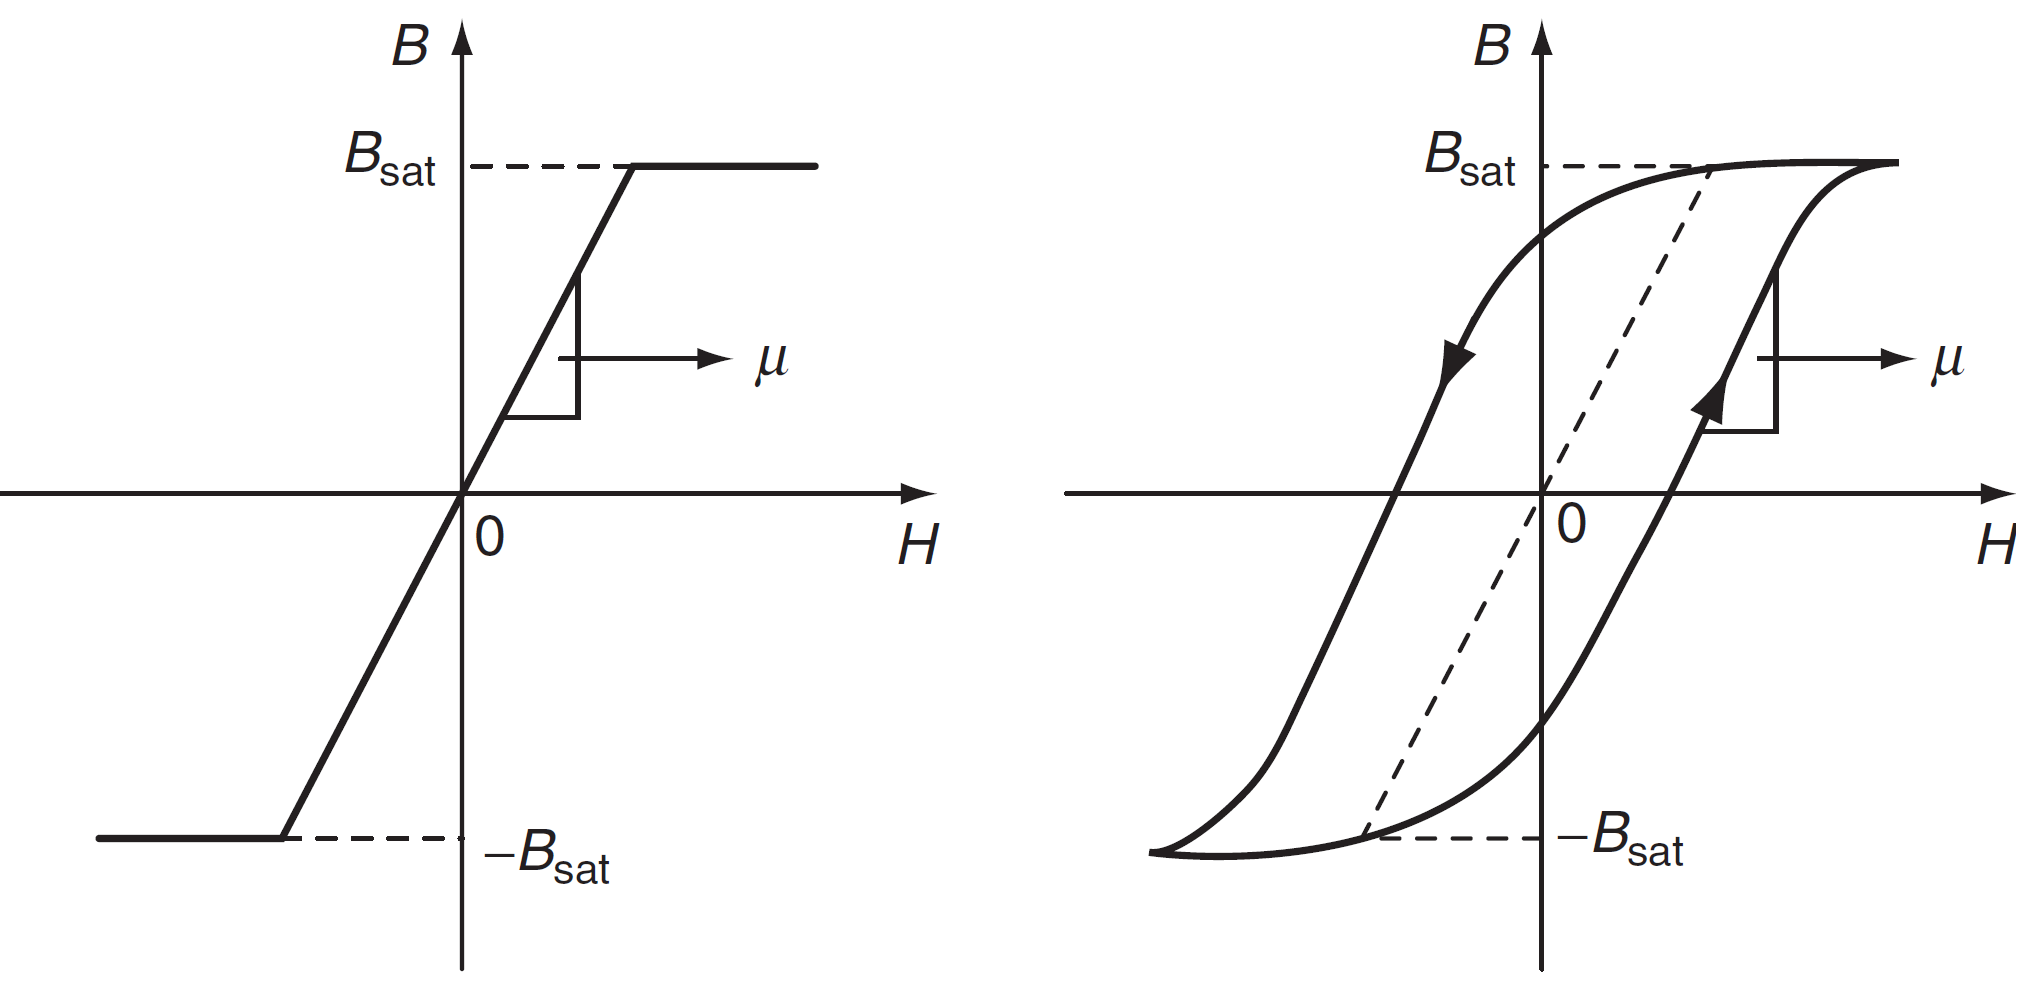
\includegraphics[width=\linewidth]{fig/lec07/BH_loop.png}
                \caption{Piecewise-linear and practical $B$--$H$ characteristics, including hysteresis loop behaviour. Adapted from Umanand, \textit{Power Electronics: Essentials and Applications}}
            \end{figure}
        \end{column}
    \end{columns}
\end{frame}


%%%%%%%%%%%%%%%%%%%%%%%%%%%%%%%%%%%%%%%%%%%%%%%%%%%%%%%%%%%%%
%% Eddy current loss
%%%%%%%%%%%%%%%%%%%%%%%%%%%%%%%%%%%%%%%%%%%%%%%%%%%%%%%%%%%%%
\begin{frame}
    \frametitle{Eddy-Current Loss in the Core}

    \begin{columns}
        \begin{column}{0.58\textwidth}
            A time-varying magnetic flux induces voltage inside conductive magnetic material. This voltage drives circulating currents called eddy currents. Eddy currents cause resistive heating inside the core:
            \begin{align}
                P_{\mathrm{eddy}} \sim i_{\mathrm{eddy}}^2 R_{\mathrm{core}}
            \end{align}
            Eddy-current loss increases strongly with frequency. This is why:
            \begin{itemize}
                \item Laminated steel is used at low line frequency.
                \item Ferrites are preferred at high frequency.
                \item Nanocrystalline and amorphous materials require careful loss evaluation.
            \end{itemize}
            High electrical resistivity of ferrite suppresses core eddy currents.
        \end{column}

        \begin{column}{0.38\textwidth}
            \begin{figure}
                \centering
                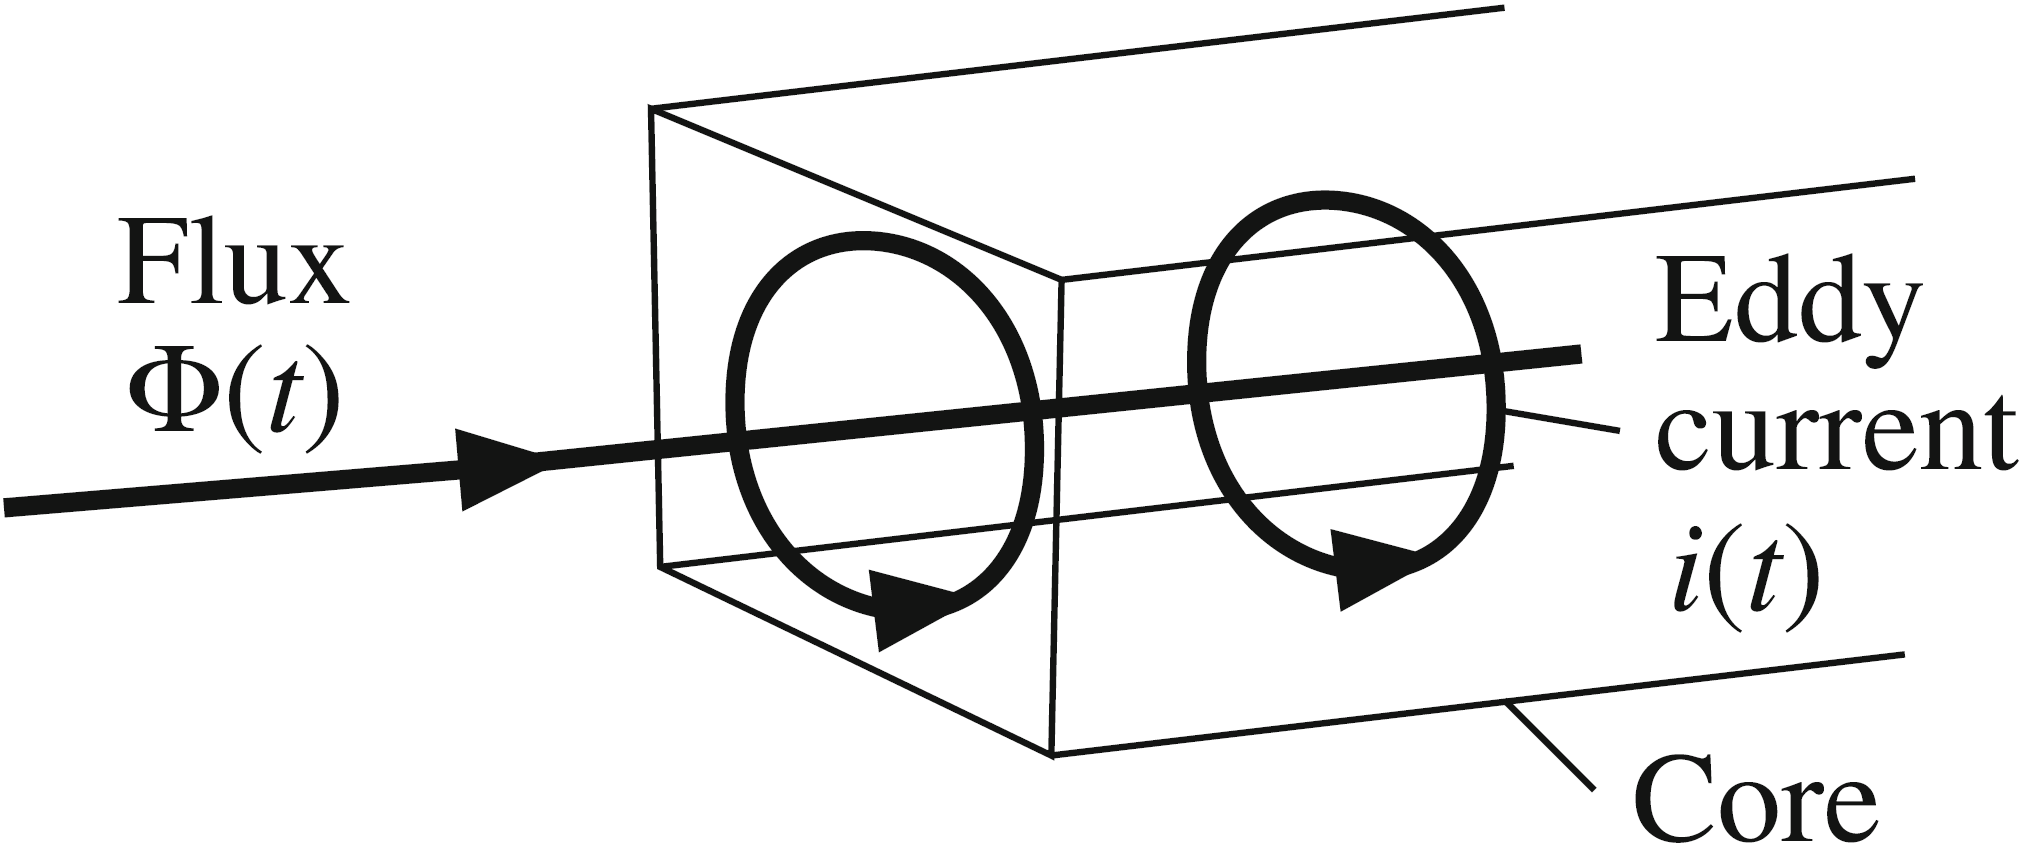
\includegraphics[width=\linewidth]{fig/lec07/eddy_current.png}
                \caption{Eddy currents induced in a magnetic core by time-varying flux. Adapted from Erickson and Maksimovi\'c, \textit{Fundamentals of Power Electronics}, 3rd edition}
            \end{figure}
        \end{column}
    \end{columns}
\end{frame}


%%%%%%%%%%%%%%%%%%%%%%%%%%%%%%%%%%%%%%%%%%%%%%%%%%%%%%%%%%%%%
%% Skin and proximity
%%%%%%%%%%%%%%%%%%%%%%%%%%%%%%%%%%%%%%%%%%%%%%%%%%%%%%%%%%%%%
\begin{frame}
    \frametitle{Skin Effect and Proximity Effect}

    \begin{columns}
        \begin{column}{0.58\textwidth}
            AC winding loss is usually much larger than DC winding loss at high frequency.
            \textbf{Skin effect:}
            \begin{itemize}
                \item Current crowds near the surface of a conductor.
                \item Effective conducting area decreases.
                \item AC resistance increases with frequency.
            \end{itemize}
            \begin{align}
                \delta = \sqrt{\frac{2\rho}{\omega\mu}}
            \end{align}
            \textbf{Proximity effect:}
            \begin{itemize}
                \item Nearby conductors impose additional magnetic fields.
                \item Current distribution becomes non-uniform.
                \item Multilayer windings can suffer severe AC resistance increase.
            \end{itemize}
        \end{column}
        \begin{column}{0.38\textwidth}
            \begin{figure}
                \centering
                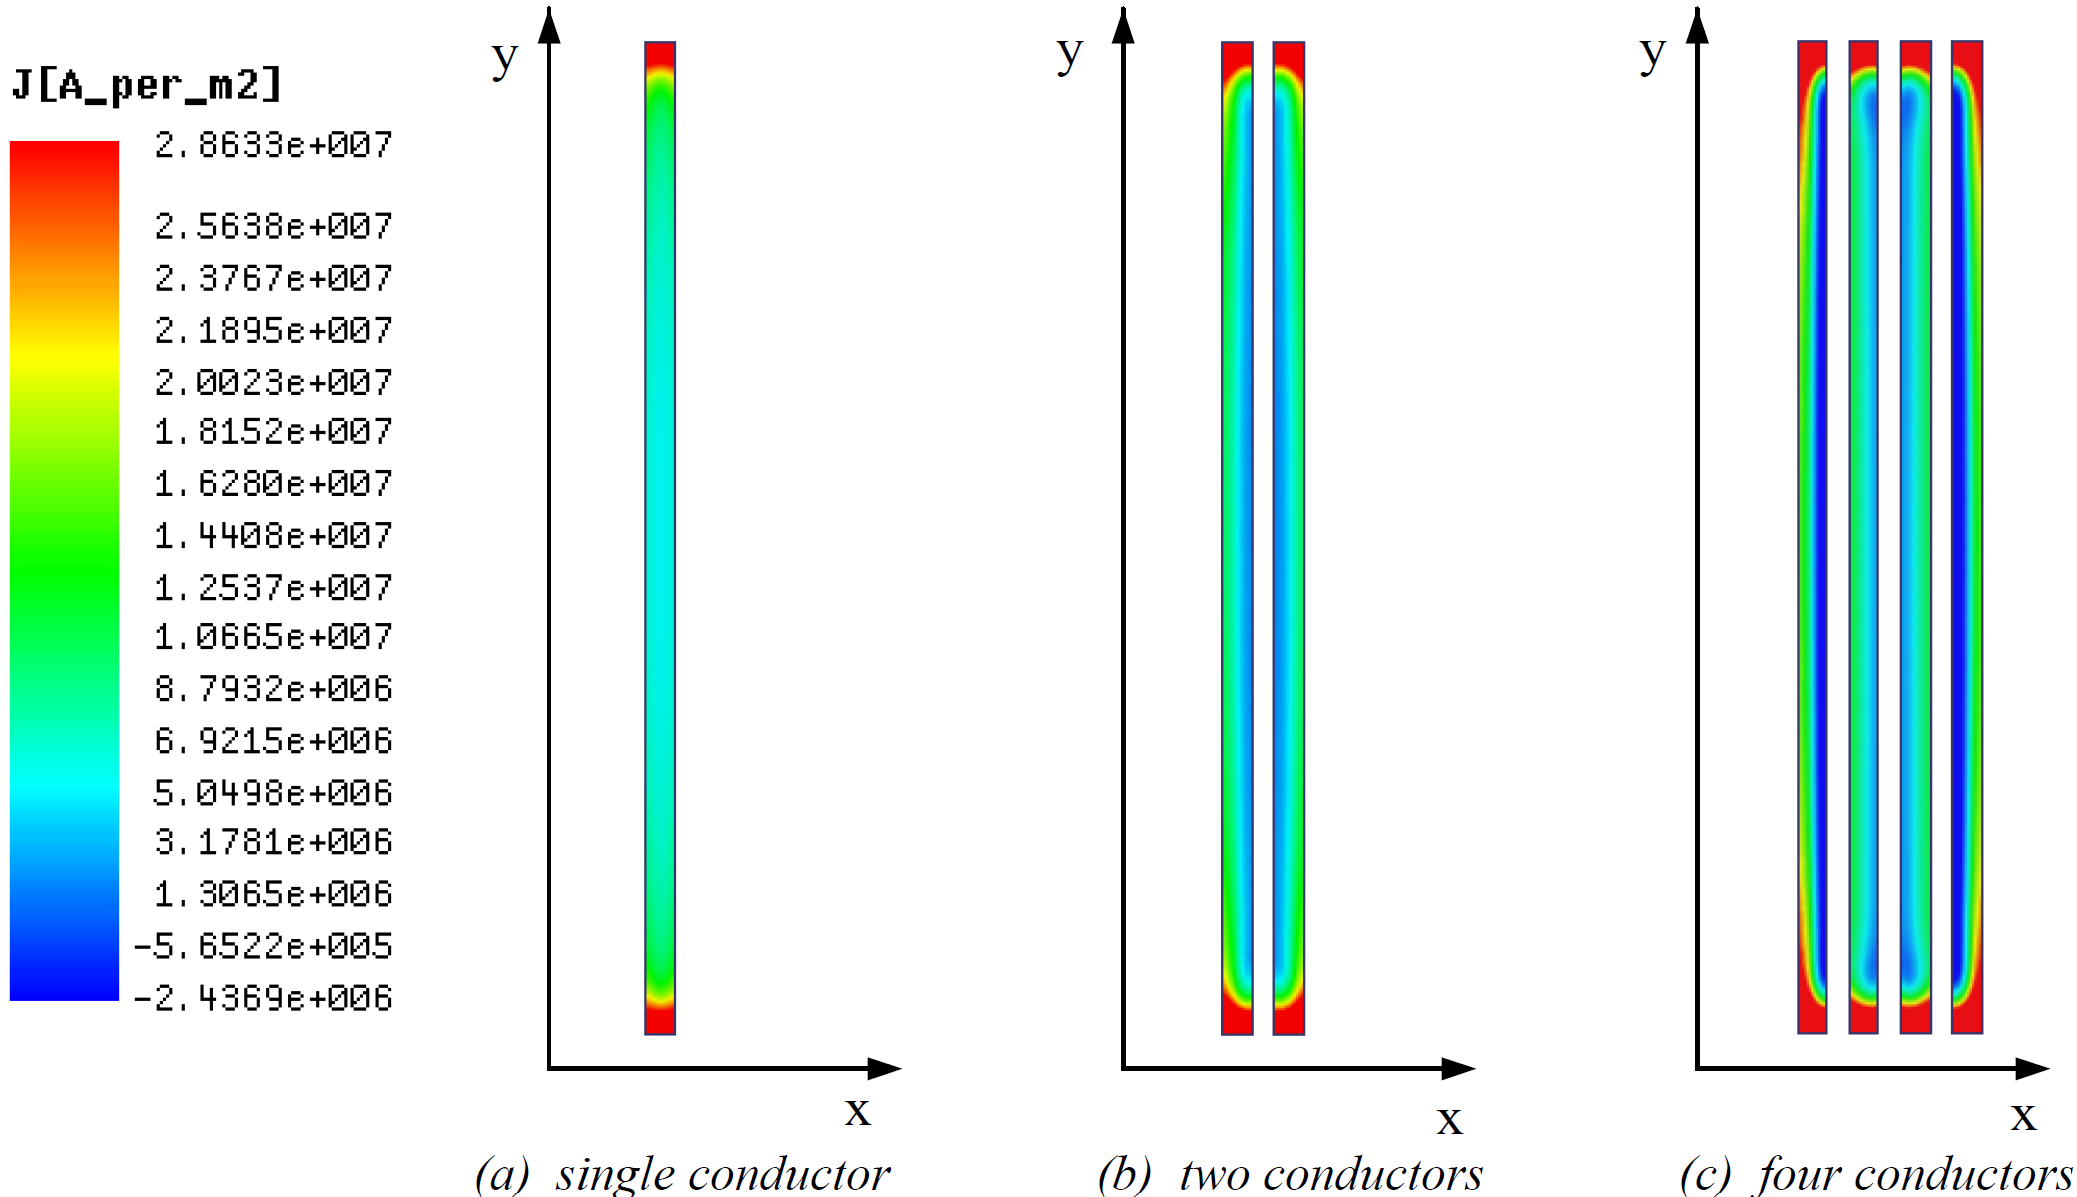
\includegraphics[width=\linewidth]{fig/lec07/current_density_distribution.png}
                \caption{Current-density distribution in single and multiple conductors showing skin and proximity effects. Adapted from Ouyang, \textit{Advances in Planar and Integrated Magnetics}}
            \end{figure}
        \end{column}
    \end{columns}
\end{frame}


%%%%%%%%%%%%%%%%%%%%%%%%%%%%%%%%%%%%%%%%%%%%%%%%%%%%%%%%%%%%%
%% Fringing and gapped inductor loss
%%%%%%%%%%%%%%%%%%%%%%%%%%%%%%%%%%%%%%%%%%%%%%%%%%%%%%%%%%%%%
\begin{frame}
    \frametitle{Fringing-Field Loss in Gapped Inductors}
            In gapped inductors and flyback magnetic components, the air gap stores most of the recoverable magnetic energy.

            \vspace{0.15cm}

            However, the gap also creates fringing flux. This flux can cut nearby windings and induce additional eddy-current loss.

            \vspace{0.15cm}

            Practical consequences:
            \begin{itemize}
                \item Local hot spots near the air gap
                \item Increased AC resistance
                \item Strong dependence on gap location
                \item Need for keep-away regions around the gap
            \end{itemize}

            \vspace{0.15cm}

            Distributed gaps or moving the gap away from windings can reduce fringing-field loss.

\end{frame}

\begin{frame}
    \frametitle{Fringing-Field Loss in Gapped Inductors}
            \begin{figure}
                \centering
                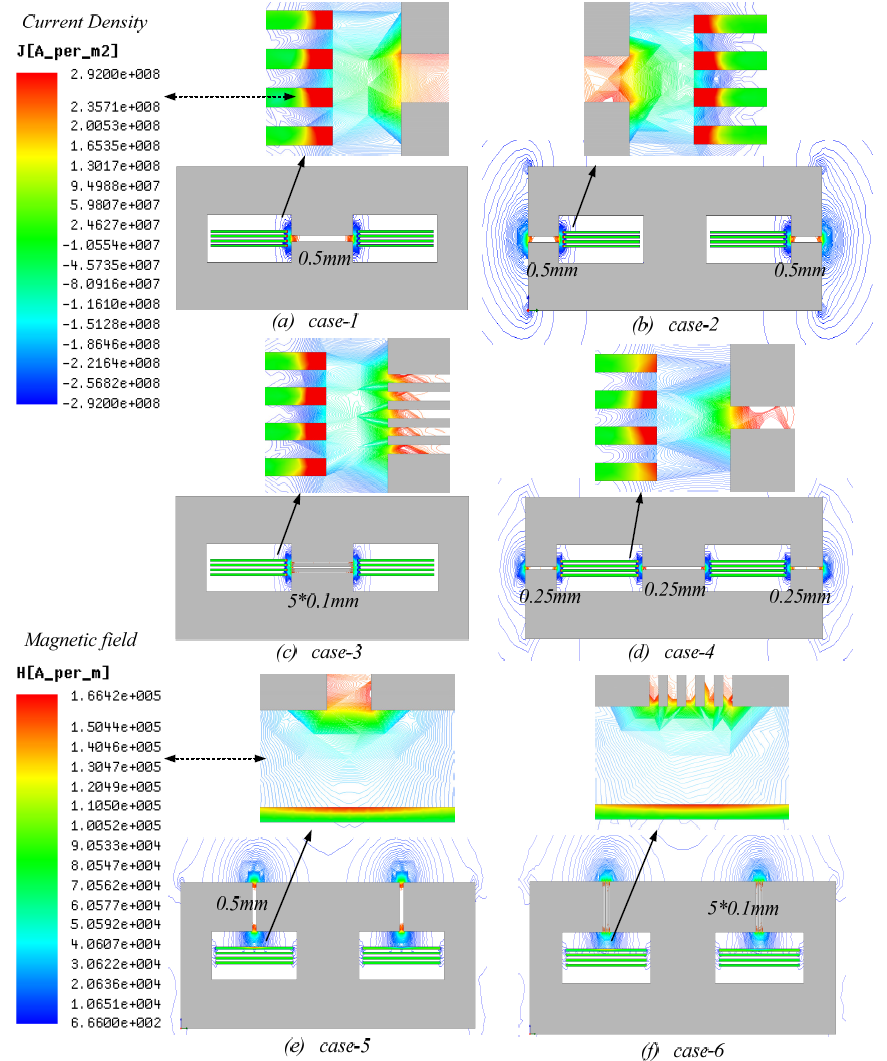
\includegraphics[width=0.3\linewidth]{fig/lec07/fringing_gap_cases.png}
                \caption{Comparison of fringing effects for different air-gap arrangements using 2-D FEA. Adapted from Ouyang, \textit{Advances in Planar and Integrated Magnetics}}
            \end{figure}
\end{frame}
%%%%%%%%%%%%%%%%%%%%%%%%%%%%%%%%%%%%%%%%%%%%%%%%%%%%%%%%%%%%%
%% Copper vs core loss trade-off
%%%%%%%%%%%%%%%%%%%%%%%%%%%%%%%%%%%%%%%%%%%%%%%%%%%%%%%%%%%%%
\begin{frame}
    \frametitle{Copper Loss versus Core Loss Trade-off}

    \begin{columns}
        \begin{column}{0.58\textwidth}
            Magnetic design is an optimization problem, not a single-equation calculation. If the designer increases the flux density:
            \begin{itemize}
                \item Fewer turns are required.
                \item Winding length decreases.
                \item Copper loss may decrease.
                \item Core loss increases.
            \end{itemize}
            If the designer decreases the flux density:
            \begin{itemize}
                \item More turns are required.
                \item Copper loss may increase.
                \item Core loss decreases.
                \item Core may become larger.
            \end{itemize}
        \end{column}

        \begin{column}{0.38\textwidth}
            \begin{align}
                P_{\mathrm{total}} =
                P_{\mathrm{core}} + P_{\mathrm{Cu,dc}} + P_{\mathrm{Cu,ac}}
            \end{align}
            \begin{block}{Design Objective}
                \small
                Do not minimize core loss alone or copper loss alone.

                \vspace{0.15cm}

                Select geometry, turns, flux density, and winding layout to minimize total loss subject to thermal, insulation, and parasitic constraints.
            \end{block}
        \end{column}
    \end{columns}
\end{frame}


%%%%%%%%%%%%%%%%%%%%%%%%%%%%%%%%%%%%%%%%%%%%%%%%%%%%%%%%%%%%%
%% Module 5
%%%%%%%%%%%%%%%%%%%%%%%%%%%%%%%%%%%%%%%%%%%%%%%%%%%%%%%%%%%%%
\begin{frame}
\begin{center}
  \textbf{\Huge{Modern Magnetics}}\\[0.4cm]
  \textbf{\Large{Planar, Integrated, MHz, and Thermally-Aware Designs}}
\end{center}
\end{frame}


%%%%%%%%%%%%%%%%%%%%%%%%%%%%%%%%%%%%%%%%%%%%%%%%%%%%%%%%%%%%%
%% Planar magnetics
%%%%%%%%%%%%%%%%%%%%%%%%%%%%%%%%%%%%%%%%%%%%%%%%%%%%%%%%%%%%%
\begin{frame}
    \frametitle{Planar Magnetics}

    \begin{columns}
        \begin{column}{0.40\textwidth}
            Planar magnetics use flat copper windings and low-profile magnetic cores instead of conventional round-wire windings on bobbins.

            Advantages:
            \begin{itemize}
                \item Low profile
                \item Good repeatability
                \item Improved thermal spreading
                \item Easier interleaving
                \item Controlled parasitics
                \item Suitable for automated manufacturing
            \end{itemize}
        \end{column}

        \begin{column}{0.60\textwidth}
            \begin{figure}
                \centering
                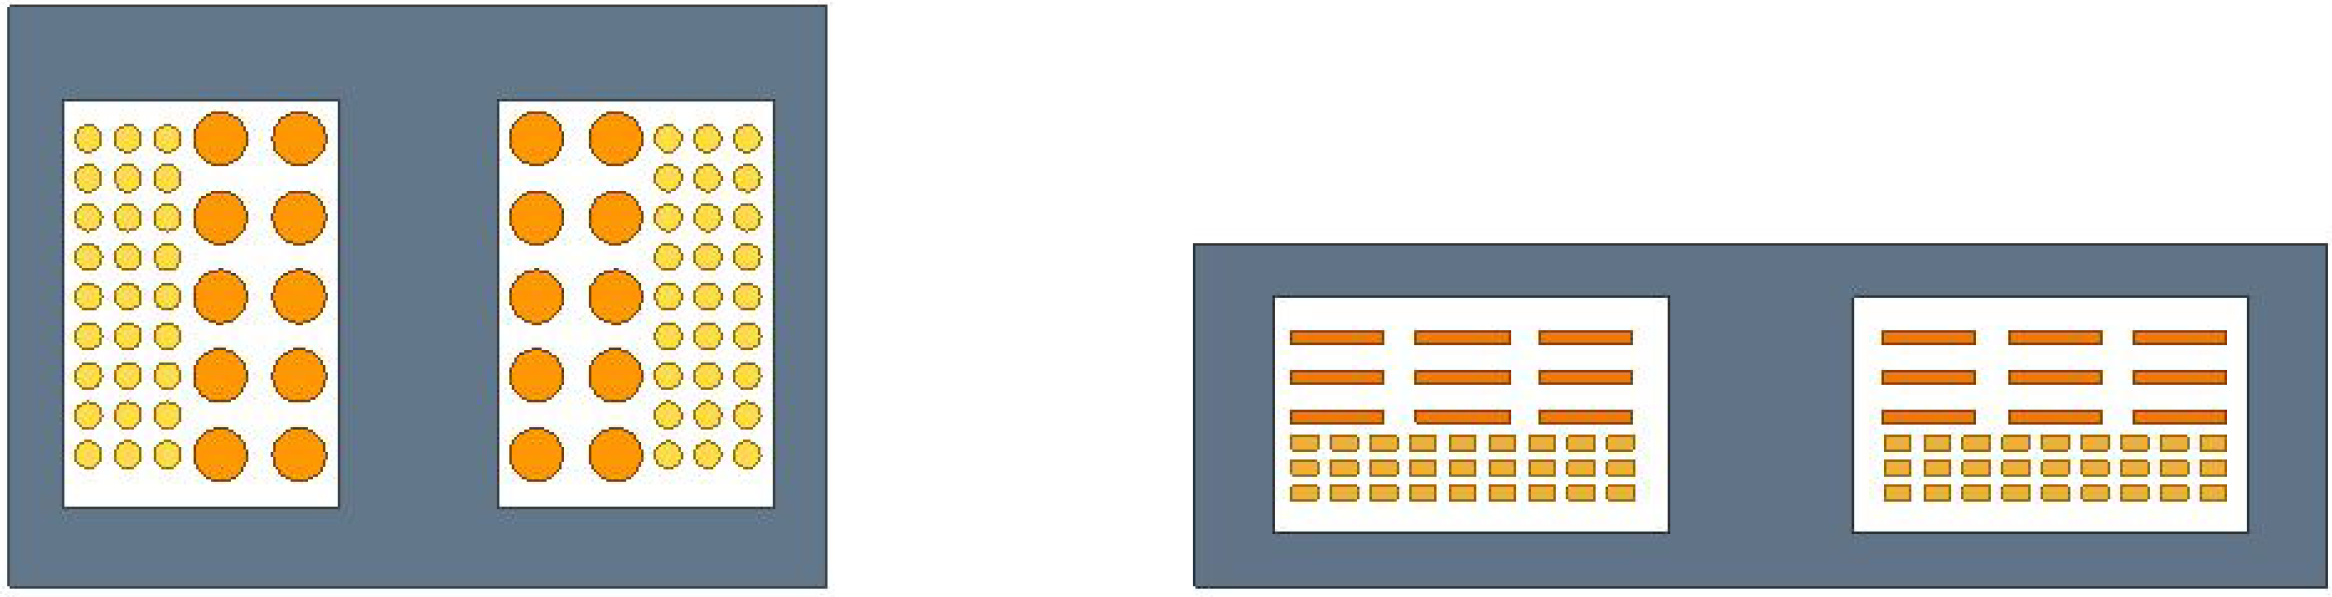
\includegraphics[width=\linewidth]{fig/lec07/standard_vs_planar_cross_section.png}
                \caption{Comparison of standard transformer and planar transformer cross-section structures. Adapted from STMicroelectronics, \textit{How Planar Magnetics Improve Performance in Power Electronics}}
            \end{figure}
        \end{column}
    \end{columns}
\end{frame}


%%%%%%%%%%%%%%%%%%%%%%%%%%%%%%%%%%%%%%%%%%%%%%%%%%%%%%%%%%%%%
%% Planar magnetics
%%%%%%%%%%%%%%%%%%%%%%%%%%%%%%%%%%%%%%%%%%%%%%%%%%%%%%%%%%%%%
\begin{frame}
    \frametitle{Planar Magnetics}
    \begin{columns}
        \begin{column}{0.38\textwidth}
            Drawbacks:
            \begin{itemize}
                \item Larger footprint
                \item Lower copper fill factor
                \item Limited number of turns
                \item Higher interwinding capacitance
                \item PCB manufacturing constraints
            \end{itemize}
        \end{column}

        \begin{column}{0.60\textwidth}
            \begin{figure}
                \centering
                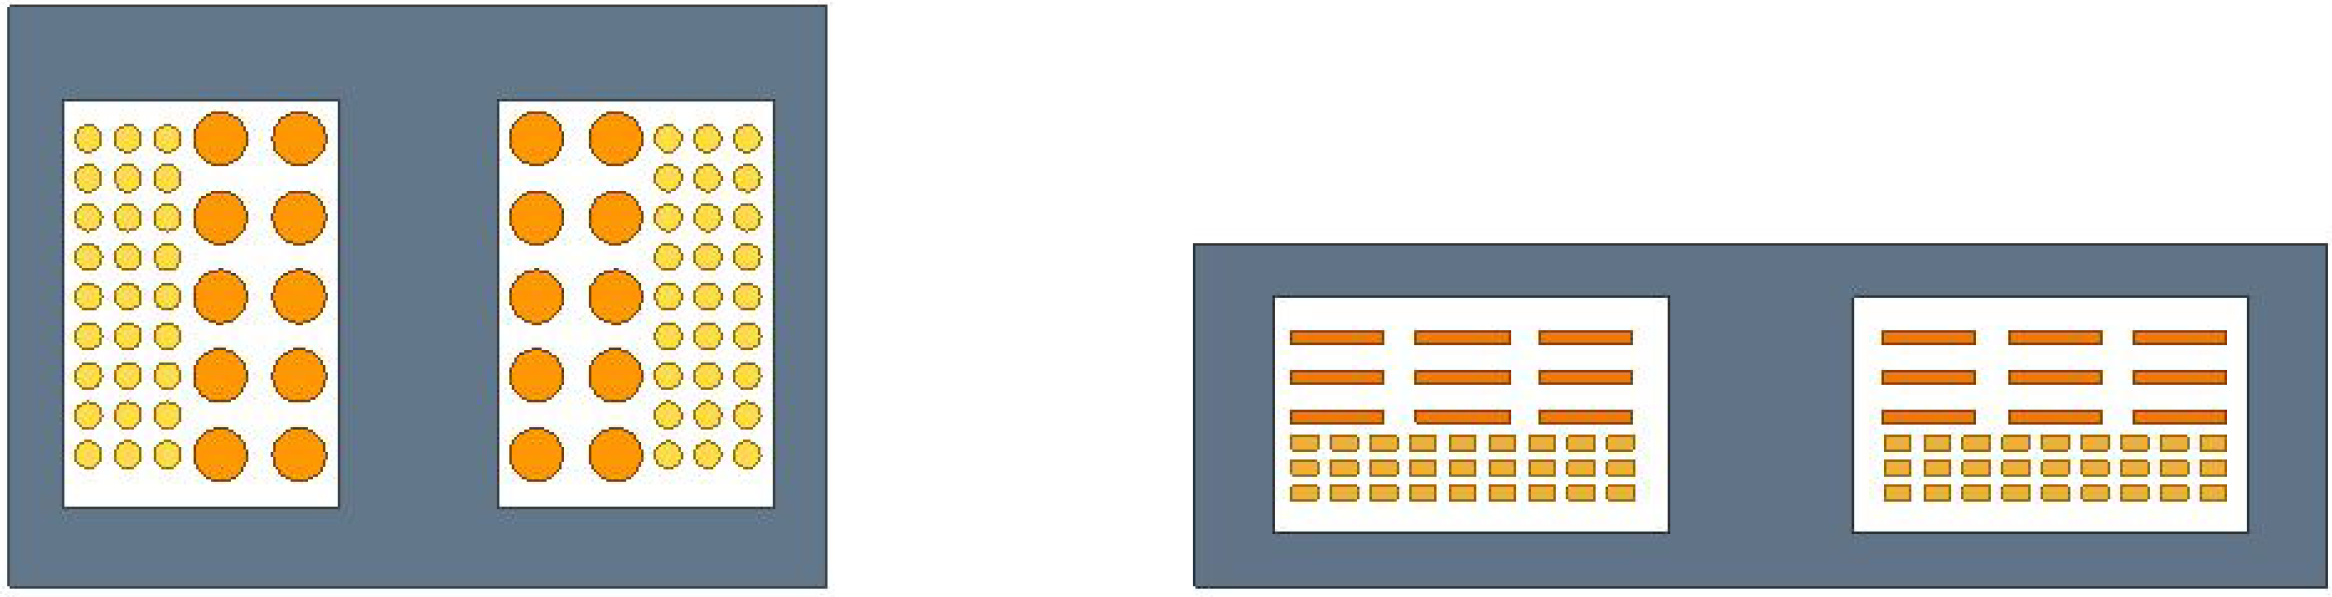
\includegraphics[width=\linewidth]{fig/lec07/standard_vs_planar_cross_section.png}
                \caption{Comparison of standard transformer and planar transformer cross-section structures. Adapted from STMicroelectronics, \textit{How Planar Magnetics Improve Performance in Power Electronics}}
            \end{figure}
        \end{column}
    \end{columns}
\end{frame}


%%%%%%%%%%%%%%%%%%%%%%%%%%%%%%%%%%%%%%%%%%%%%%%%%%%%%%%%%%%%%
%% Planar construction
%%%%%%%%%%%%%%%%%%%%%%%%%%%%%%%%%%%%%%%%%%%%%%%%%%%%%%%%%%%%%
\begin{frame}
    \frametitle{Planar Transformer Construction}

    \begin{columns}
        \begin{column}{0.58\textwidth}
            A planar transformer is usually built from:
            \begin{itemize}
                \item Low-profile ferrite core
                \item PCB or flexible-PCB winding layers
                \item Copper traces or stamped copper turns
                \item Insulation layers
                \item Vias or pins for interconnection
            \end{itemize}

            The geometry fixes the winding positions very precisely. Therefore, leakage inductance, capacitance, and resistance are more repeatable than in manually wound transformers.

            \vspace{0.15cm}

            This is a major advantage in resonant converters, where leakage inductance and parasitic capacitance can strongly affect the gain and EMI behaviour.
        \end{column}

        \begin{column}{0.38\textwidth}
            \begin{figure}
                \centering
                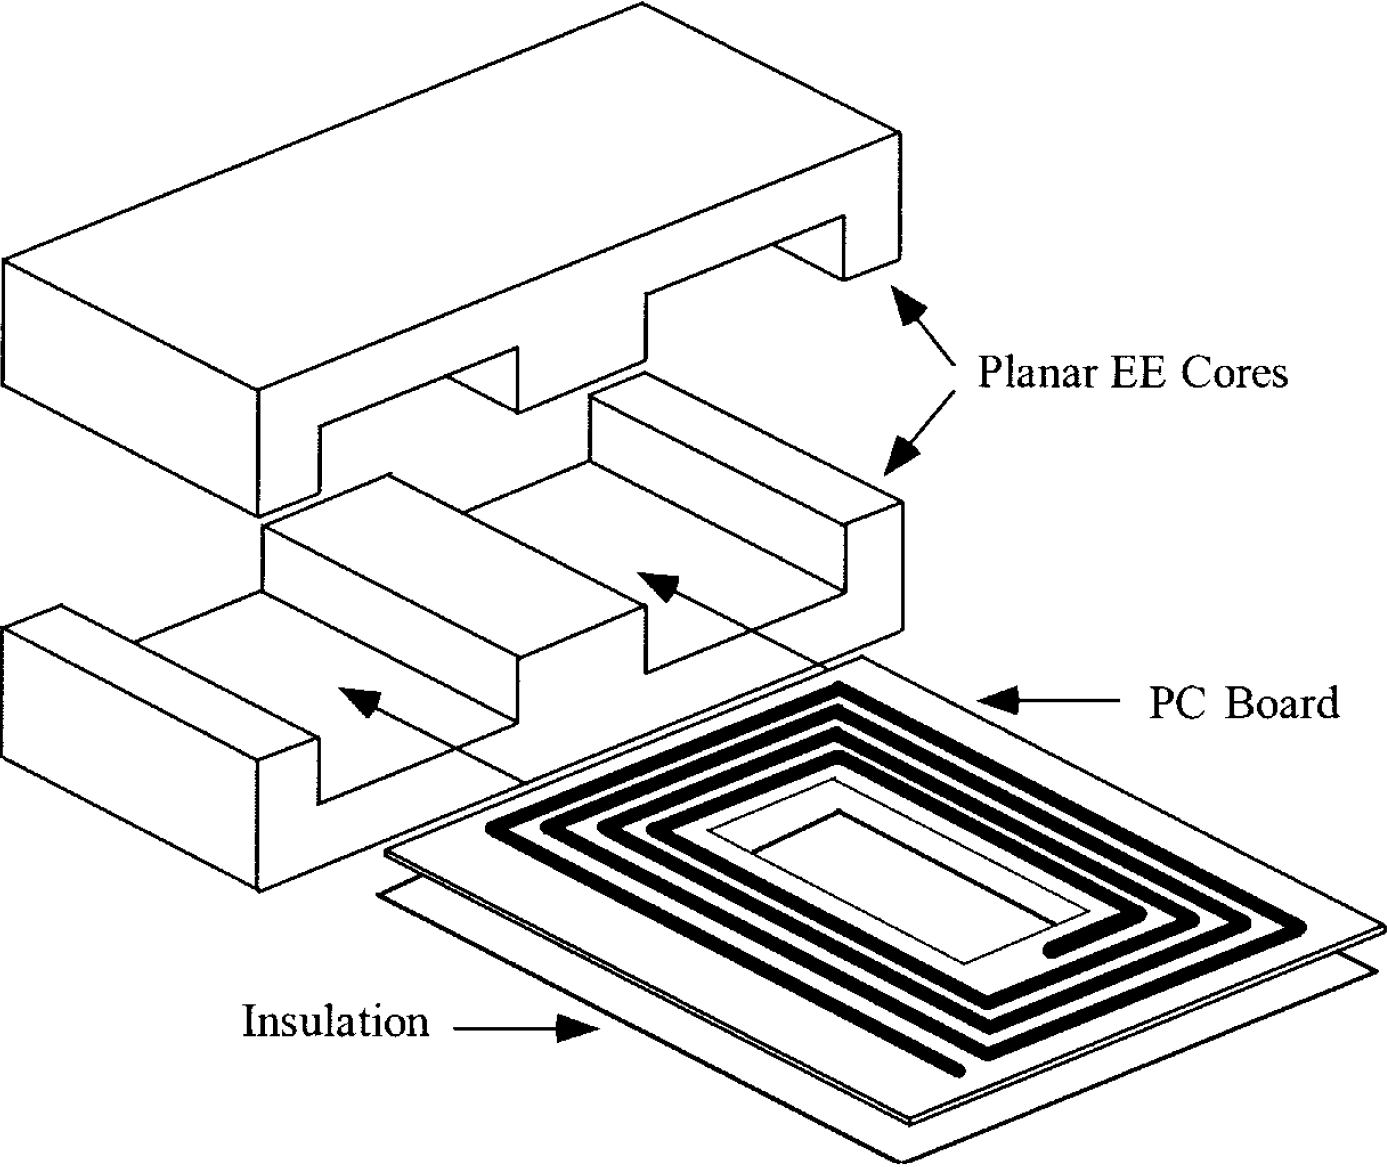
\includegraphics[width=\linewidth]{fig/lec07/planar_EE_perspective.png}
                \caption{Perspective view of a typical EE planar transformer using PC-board windings and planar EE cores. Adapted from \textit{Transformer and Inductor Design Handbook}}
            \end{figure}
        \end{column}
    \end{columns}
\end{frame}


%%%%%%%%%%%%%%%%%%%%%%%%%%%%%%%%%%%%%%%%%%%%%%%%%%%%%%%%%%%%%
%% PCB integrated transformer
%%%%%%%%%%%%%%%%%%%%%%%%%%%%%%%%%%%%%%%%%%%%%%%%%%%%%%%%%%%%%
\begin{frame}
    \frametitle{PCB-Integrated Planar Transformer}

    \begin{columns}
        \begin{column}{0.58\textwidth}
            Planar magnetics can be integrated into the main converter PCB. This reduces separate component count and improves mechanical repeatability.

            \vspace{0.15cm}

            A PCB-integrated transformer typically uses:
            \begin{itemize}
                \item Multiple copper layers for primary and secondary turns
                \item Vias for layer-to-layer connections
                \item Ferrite core halves inserted around the PCB
                \item Controlled insulation layers between primary and secondary
            \end{itemize}
        \end{column}

        \begin{column}{0.38\textwidth}
            \begin{figure}
                \centering
                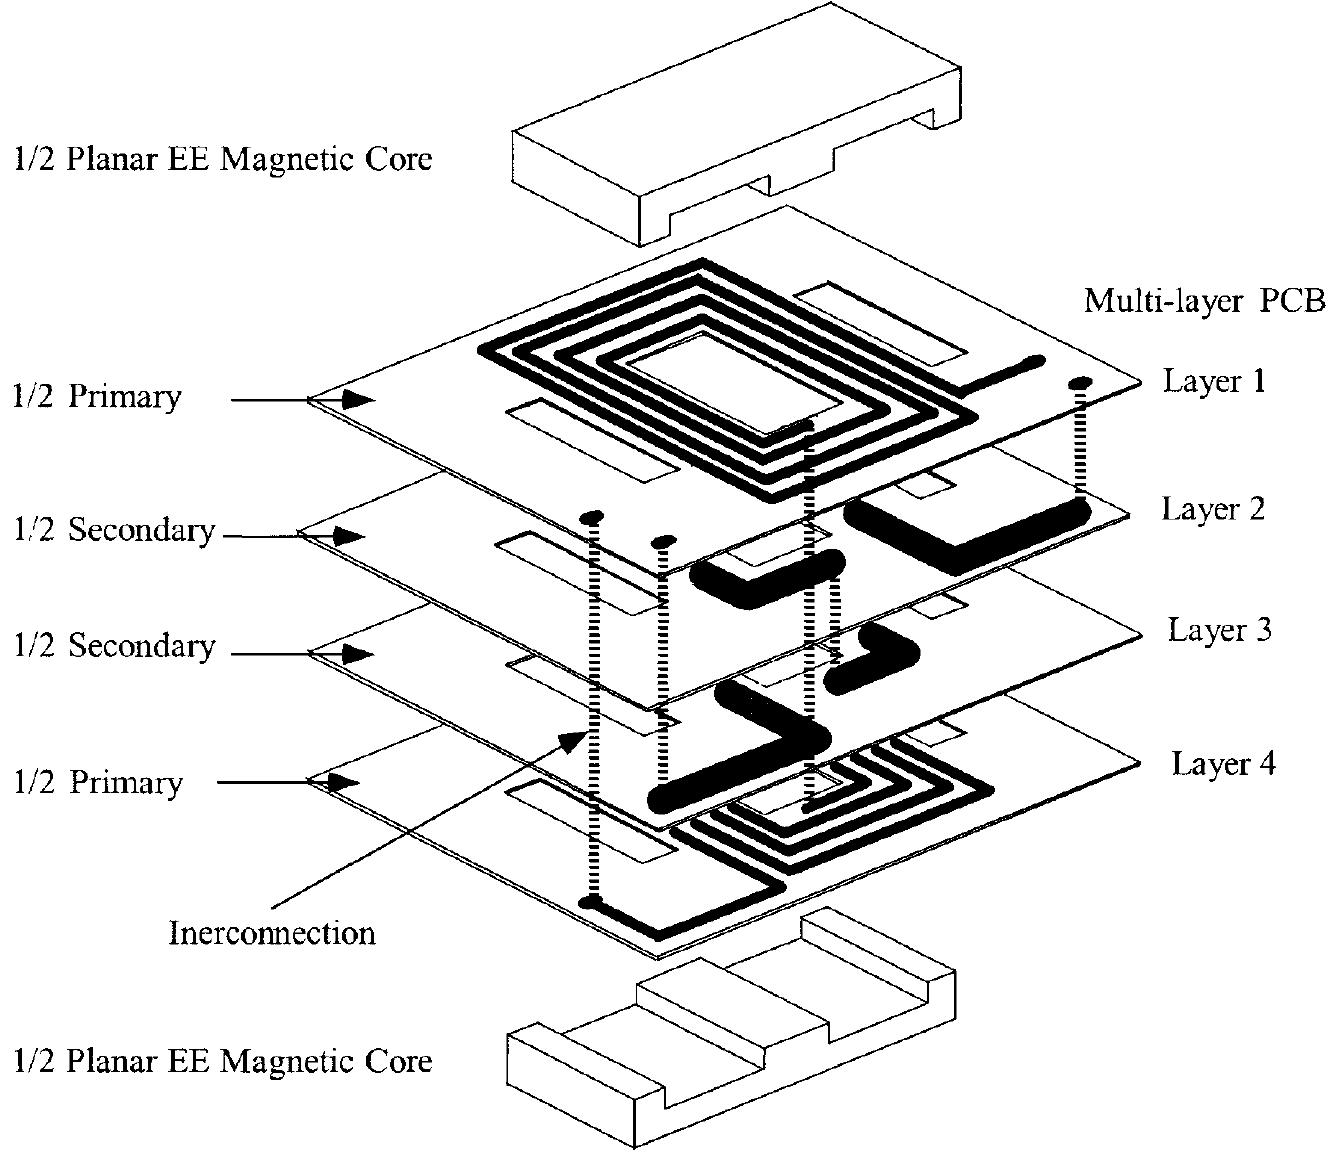
\includegraphics[width=\linewidth]{fig/lec07/planer_trans.png}
                \caption{Planar transformer integrated into the main PC board and final assembly. Adapted from \textit{Transformer and Inductor Design Handbook}, Chapter 20, Figs. 20-5 and 20-6.}
            \end{figure}
        \end{column}
    \end{columns}
\end{frame}



%%%%%%%%%%%%%%%%%%%%%%%%%%%%%%%%%%%%%%%%%%%%%%%%%%%%%%%%%%%%%
%% PCB integrated transformer
%%%%%%%%%%%%%%%%%%%%%%%%%%%%%%%%%%%%%%%%%%%%%%%%%%%%%%%%%%%%%
\begin{frame}
    \frametitle{PCB-Integrated Planar Transformer}

    \begin{columns}
        \begin{column}{0.58\textwidth}
            The design challenge is to simultaneously satisfy:
            \begin{itemize}
                \item Copper loss limit
                \item Core loss limit
                \item Isolation requirement
                \item Leakage and capacitance targets
                \item PCB manufacturing rules
            \end{itemize}
        \end{column}

        \begin{column}{0.38\textwidth}
            \begin{figure}
                \centering
                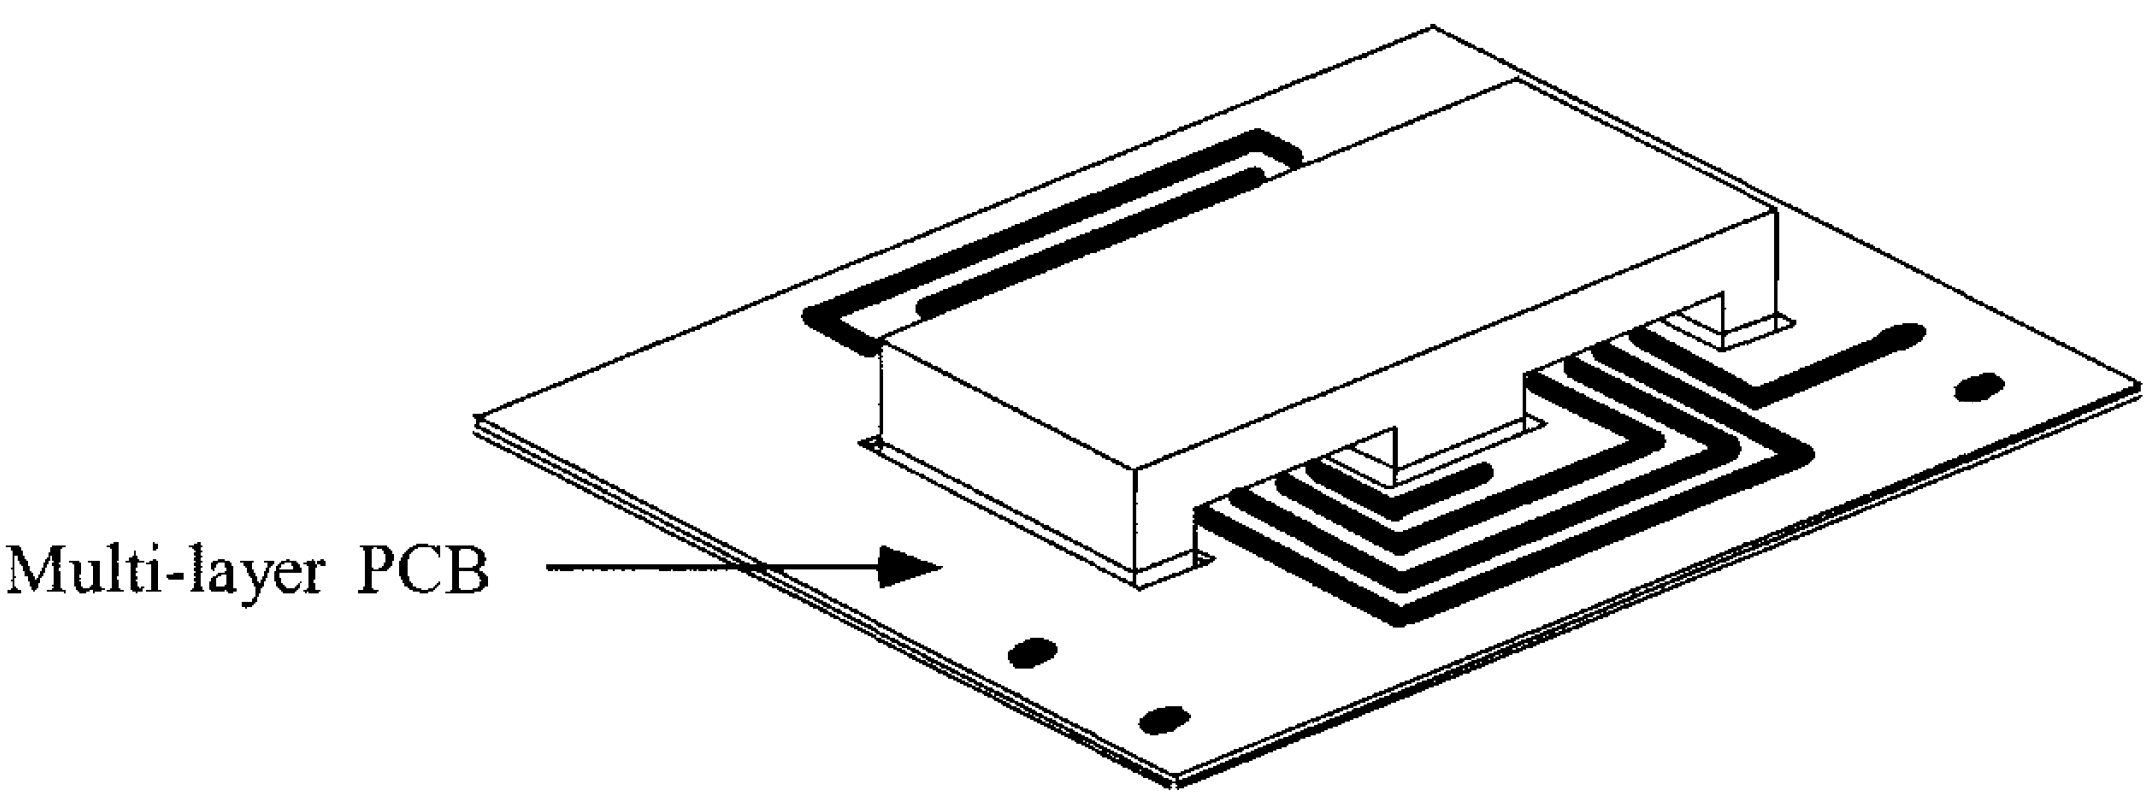
\includegraphics[width=\linewidth]{fig/lec07/planar_trans_assembly.png}
                \caption{Planar transformer integrated into the main PC board and final assembly. Adapted from \textit{Transformer and Inductor Design Handbook}, Chapter 20, Figs. 20-5 and 20-6.}
            \end{figure}
        \end{column}
    \end{columns}
\end{frame}


%%%%%%%%%%%%%%%%%%%%%%%%%%%%%%%%%%%%%%%%%%%%%%%%%%%%%%%%%%%%%
%% Modeling planar magnetics
%%%%%%%%%%%%%%%%%%%%%%%%%%%%%%%%%%%%%%%%%%%%%%%%%%%%%%%%%%%%%
\begin{frame}
    \frametitle{Modeling Planar Magnetics}

    \begin{columns}
        \begin{column}{0.58\textwidth}
            Planar magnetics are attractive, but they require accurate modeling because skin effect, proximity effect, vias, gaps, and layer coupling strongly influence performance.

            The Modular Layer Model represents each PCB layer as an impedance network. This allows the designer to predict:
            \begin{itemize}
                \item Current sharing
                \item AC resistance
                \item Winding impedance
                \item Stored reactive energy
                \item Field distribution
                \item Loss distribution
            \end{itemize}

            \vspace{0.15cm}
        \end{column}

        \begin{column}{0.38\textwidth}
            \begin{figure}
                \centering
                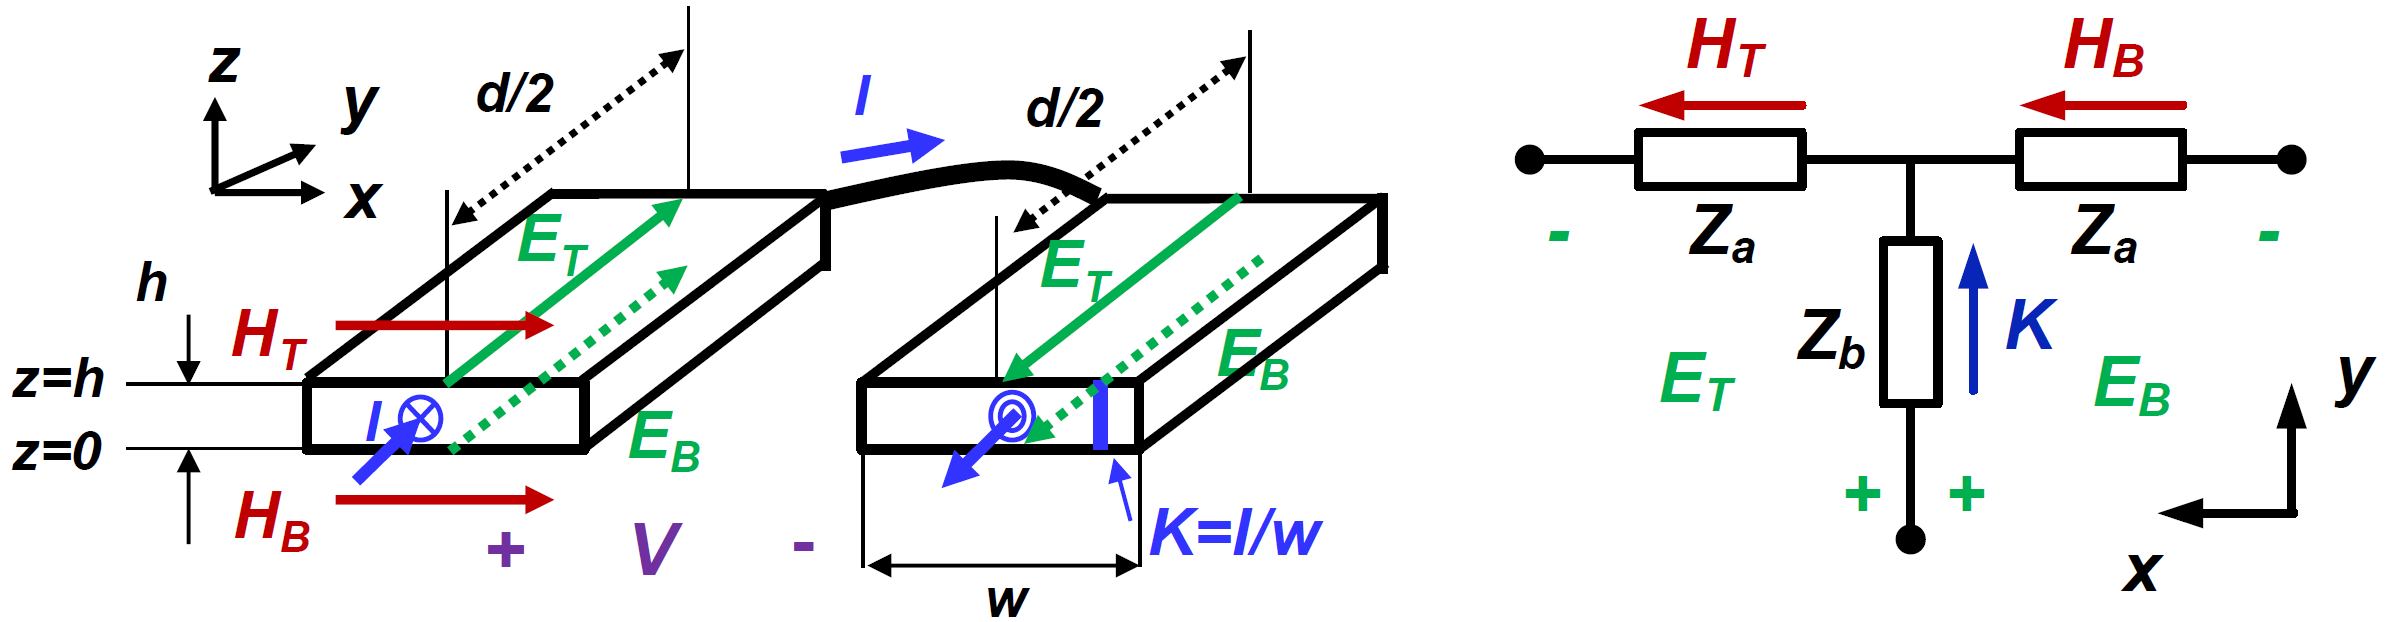
\includegraphics[width=\linewidth]{fig/lec07/one_turn_layer_model.png}
                \caption{One-turn planar layer and its three-terminal impedance network. Adapted from Chen et al., \textit{A Systematic Approach to Modeling Impedances and Current Distribution in Planar Magnetics}}
            \end{figure}
        \end{column}
    \end{columns}
Such models are useful before moving to detailed 2-D or 3-D finite-element simulations.
\end{frame}


%%%%%%%%%%%%%%%%%%%%%%%%%%%%%%%%%%%%%%%%%%%%%%%%%%%%%%%%%%%%%
%% MHz magnetics
%%%%%%%%%%%%%%%%%%%%%%%%%%%%%%%%%%%%%%%%%%%%%%%%%%%%%%%%%%%%%
\begin{frame}
    \frametitle{MHz Magnetics}

    \begin{columns}
        \begin{column}{0.58\textwidth}
            Wide-bandgap devices enable switching frequencies from hundreds of kHz into the MHz range.

            Higher frequency can reduce magnetic size because volt-seconds per cycle decrease:
            \begin{align}
                \Delta B =
                \frac{1}{N A_c}\int v(t)\,dt
            \end{align}
            However, MHz magnetics face severe constraints:
            \begin{itemize}
                \item Core loss rises rapidly with frequency
                \item AC winding resistance increases
                \item Parasitic capacitance becomes circuit-relevant
                \item Thermal paths become critical
                \item Layout and EMI dominate behaviour
            \end{itemize}
        \end{column}
        \begin{column}{0.38\textwidth}
            Ferrites, air-core structures, PCB windings, and thin low-loss cores are often considered.
            \begin{block}{MHz Design Message}
                \small
                Increasing frequency reduces magnetic volume only if core loss, winding loss, thermal rise, and EMI remain controlled.
            \end{block}
        \end{column}
    \end{columns}
\end{frame}


%%%%%%%%%%%%%%%%%%%%%%%%%%%%%%%%%%%%%%%%%%%%%%%%%%%%%%%%%%%%%
%% Integrated magnetics
%%%%%%%%%%%%%%%%%%%%%%%%%%%%%%%%%%%%%%%%%%%%%%%%%%%%%%%%%%%%%
\begin{frame}
    \frametitle{Integrated Magnetics}
            Integrated magnetics combine multiple magnetic functions into one magnetic structure.

            Examples include:
            \begin{itemize}
                \item Transformer plus resonant inductor
                \item Transformer plus output filter inductor
                \item Coupled inductors for multiphase converters
                \item Current balancing transformer plus common inductor
            \end{itemize}

            \vspace{0.15cm}

            Potential benefits:
            \begin{itemize}
                \item Fewer magnetic components
                \item Reduced converter volume
                \item Better power density
                \item Controlled leakage or coupling
                \item Lower assembly cost
            \end{itemize}

            The main challenge is controlling flux paths so that the intended functions are coupled while unwanted interactions are avoided.
\end{frame}


%%%%%%%%%%%%%%%%%%%%%%%%%%%%%%%%%%%%%%%%%%%%%%%%%%%%%%%%%%%%%
%% Cooling
%%%%%%%%%%%%%%%%%%%%%%%%%%%%%%%%%%%%%%%%%%%%%%%%%%%%%%%%%%%%%
\begin{frame}
    \frametitle{Cooling and Thermal Paths in Magnetics}
    \begin{columns}
        \begin{column}{0.58\textwidth}
            Magnetic components must be designed thermally as well as electrically.

            Heat sources:
            \begin{itemize}
                \item Core loss
                \item DC copper loss
                \item AC winding loss
                \item Fringing-induced local loss
                \item Termination and via loss
            \end{itemize}
        \end{column}

        \begin{column}{0.38\textwidth}
            \begin{figure}
                \centering
                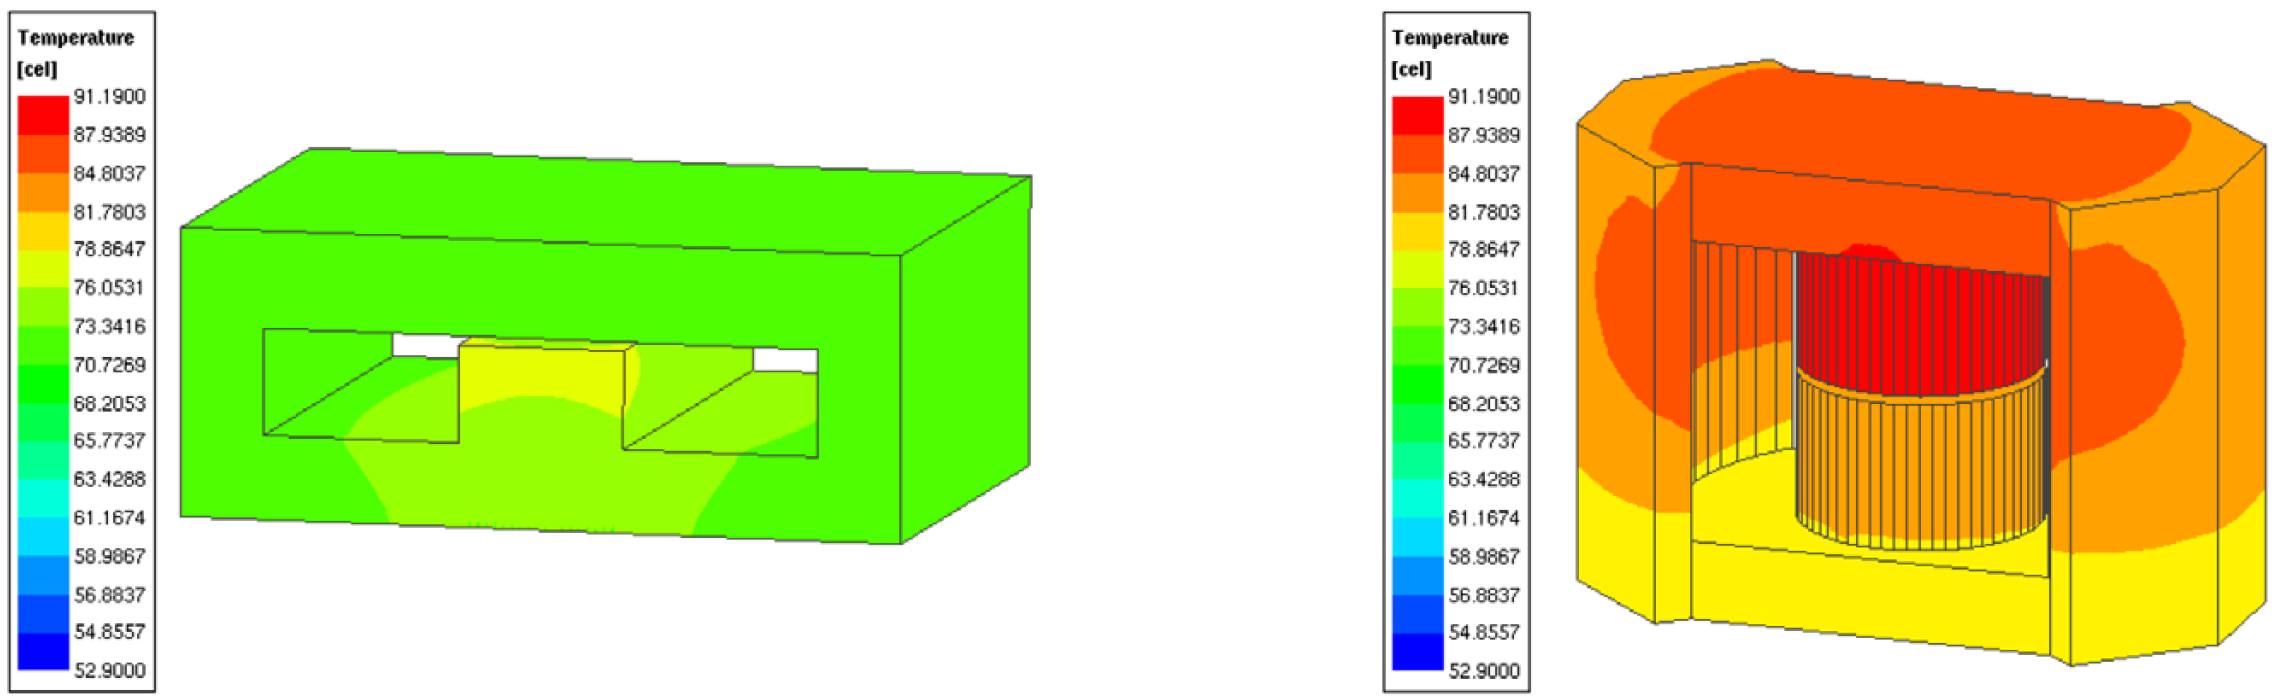
\includegraphics[width=\linewidth]{fig/lec07/thermal_profiles.png}
                \caption{Thermal comparison of planar and concentric transformers, including the effect of an aluminum dissipation plane. Adapted from STMicroelectronics, \textit{How Planar Magnetics Improve Performance in Power Electronics}, Figs. 4 and 5.}
            \end{figure}
        \end{column}
    \end{columns}
\end{frame}


%%%%%%%%%%%%%%%%%%%%%%%%%%%%%%%%%%%%%%%%%%%%%%%%%%%%%%%%%%%%%
%% Cooling
%%%%%%%%%%%%%%%%%%%%%%%%%%%%%%%%%%%%%%%%%%%%%%%%%%%%%%%%%%%%%
\begin{frame}
    \frametitle{Cooling and Thermal Paths in Magnetics}
    \begin{columns}
        \begin{column}{0.58\textwidth}
            Cooling options:
            \begin{itemize}
                \item Natural convection
                \item Forced-air cooling
                \item Heat spreading through PCB copper
                \item Aluminum baseplate or heat spreader
                \item Liquid-cooled cold plate for high power density
            \end{itemize}
            Planar cores often have favourable surface-to-volume ratio, improving heat spreading.
        \end{column}

        \begin{column}{0.38\textwidth}
            \begin{figure}
                \centering
                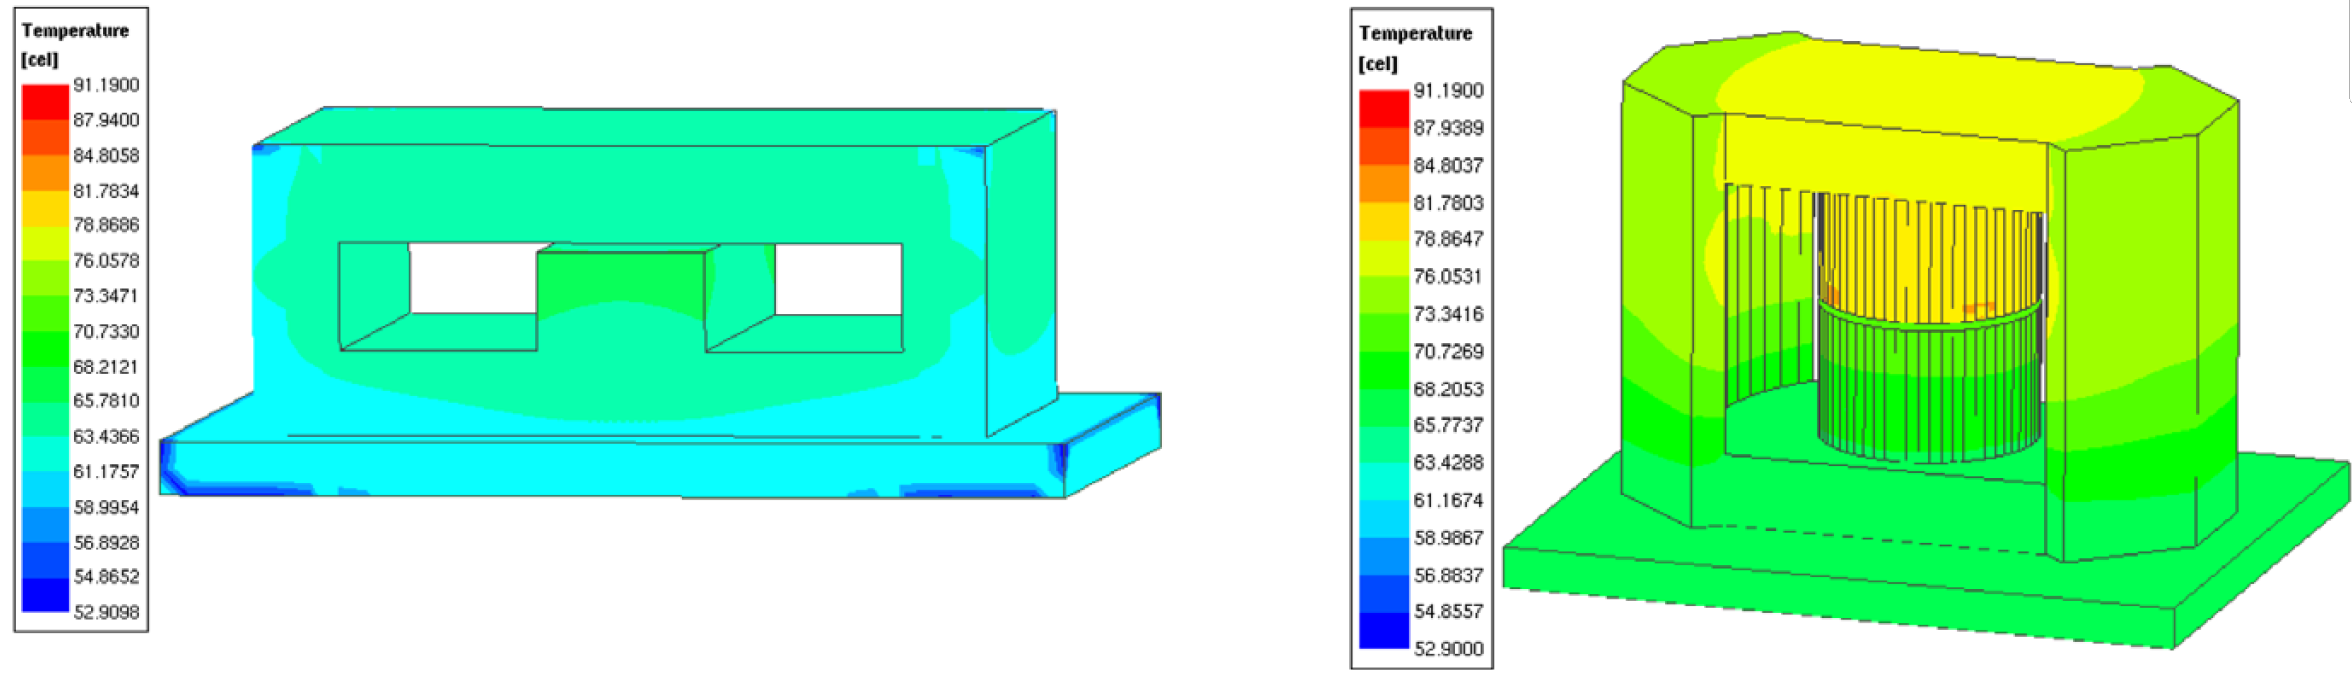
\includegraphics[width=\linewidth]{fig/lec07/thermal_profiles_2.png}
                \caption{Thermal comparison of planar and concentric transformers, including the effect of an aluminum dissipation plane. Adapted from STMicroelectronics, \textit{How Planar Magnetics Improve Performance in Power Electronics}, Figs. 4 and 5.}
            \end{figure}
        \end{column}
    \end{columns}
\end{frame}

%%%%%%%%%%%%%%%%%%%%%%%%%%%%%%%%%%%%%%%%%%%%%%%%%%%%%%%%%%%%%
%% Conventional to future magnetics
%%%%%%%%%%%%%%%%%%%%%%%%%%%%%%%%%%%%%%%%%%%%%%%%%%%%%%%%%%%%%
\begin{frame}
    \frametitle{Evolution of Magnetic Components}

    \scriptsize
    \begin{table}
        \centering
        \begin{tabular}{p{0.18\textwidth}p{0.23\textwidth}p{0.26\textwidth}p{0.22\textwidth}}
            \hline
            \textbf{Technology} & \textbf{Main Feature} & \textbf{Strength} & \textbf{Challenge}\\
            \hline
            Conventional wire-wound & Round wire on bobbin & Mature, flexible, low cost & Large size and variable parasitics\\
            Foil / Litz magnetics & Optimized conductor geometry & Lower AC loss & Manufacturing and termination complexity\\
            Planar magnetics & PCB or flat copper winding & Low profile, repeatable, good thermal spreading & Low fill factor and capacitance\\
            Integrated magnetics & Multiple magnetic functions in one core & Higher power density & Complex flux-path design\\
            Future 3-D / additive magnetics & Geometrically optimized cores and windings & Custom field shaping & Material, cost, and qualification issues\\
            \hline
        \end{tabular}
    \end{table}

    \vspace{0.15cm}

    \begin{block}{Conclusion}
        \small
        Modern magnetic design is moving from component selection toward co-design of core, winding, layout, thermal path, converter topology, and switching frequency.
    \end{block}
\end{frame}


%%%%%%%%%%%%%%%%%%%%%%%%%%%%%%%%%%%%%%%%%%%%%%%%%%%%%%%%%%%%%
%% Final magnetics summary
%%%%%%%%%%%%%%%%%%%%%%%%%%%%%%%%%%%%%%%%%%%%%%%%%%%%%%%%%%%%%
\begin{frame}
    \frametitle{Concluding Remarks on Magnetics}

    \begin{itemize}
        \item Magnetic components are not auxiliary parts; they often define the achievable efficiency, size, EMI performance, and thermal limit of a converter.

        \item Inductors, transformers, coupled inductors, flyback magnetics, and current transformers have different design objectives.

        \item Transformer design begins from volt-seconds, turns ratio, current waveforms, isolation, and thermal constraints.

        \item Winding arrangement controls leakage inductance, proximity effect, capacitance, and cooling.

        \item At high frequency, losses are dominated by core loss, skin effect, proximity effect, fringing fields, and parasitics.

        \item Planar and integrated magnetics are powerful technologies for high-power-density converters, but they require careful electromagnetic, thermal, and manufacturing co-design.

        \item For GaN and SiC converters, the magnetic component is often the bottleneck that determines whether MHz operation is practically useful.
    \end{itemize}
\end{frame}

 % Passive components in power electronics
%\section{Passive components in power electronics- Capacitors}
\title[Passive components- Capacitors]{Passive components- Capacitors}  

\begin{frame}[plain]
    \titlepage
\end{frame}

%%%%%%%%%%%%%%%%%%%%%%%%%%%%%%%%%%%%%%%%%%%%%%%%%%%%%%%%%%%%%
%% Capacitors in Power Electronics
%%%%%%%%%%%%%%%%%%%%%%%%%%%%%%%%%%%%%%%%%%%%%%%%%%%%%%%%%%%%%
\begin{frame}
\begin{center}
  \textbf{\Huge{Passive Components}}\\[0.4cm]
  \textbf{\Large{Capacitors in Power Electronics Converters}}\\[0.8cm]

  \large
  Electric-field energy storage, filtering, DC-link design, snubbers, and high-frequency applications
\end{center}
\end{frame}


%%%%%%%%%%%%%%%%%%%%%%%%%%%%%%%%%%%%%%%%%%%%%%%%%%%%%%%%%%%%%
%% Why capacitors matter
%%%%%%%%%%%%%%%%%%%%%%%%%%%%%%%%%%%%%%%%%%%%%%%%%%%%%%%%%%%%%
\begin{frame}
\frametitle{Why are Capacitors Important in Power Electronics?}

Capacitors are indispensable in power electronic converters because they store electric-field energy, control voltage ripple, supply pulsed currents, suppress transients, and shape frequency-dependent impedance.

\begin{itemize}
    \item In DC--DC converters, capacitors reduce input and output voltage ripple.
    \item In inverters and motor drives, DC-link capacitors buffer instantaneous power mismatch between source and load.
    \item In snubber circuits, capacitors limit overvoltage caused by stray inductance during switching.
    \item In EMI filters, capacitors provide low-impedance paths for high-frequency noise.
    \item In resonant converters, capacitors define the resonant frequency and circulating current.
    \item In modern SiC and GaN converters, capacitor ESR, ESL, layout, and thermal design strongly influence efficiency, EMI, and reliability.
\end{itemize}

A capacitor must therefore be selected not only by capacitance, but also by voltage rating, ripple-current capability, impedance, lifetime, temperature, and layout compatibility.

\end{frame}


%%%%%%%%%%%%%%%%%%%%%%%%%%%%%%%%%%%%%%%%%%%%%%%%%%%%%%%%%%%%%
%% Capacitor functions in converters
%%%%%%%%%%%%%%%%%%%%%%%%%%%%%%%%%%%%%%%%%%%%%%%%%%%%%%%%%%%%%
\begin{frame}
\frametitle{Main Functions of Capacitors in Power Converters}

\begin{columns}
\begin{column}{0.57\textwidth}

Capacitors appear at several positions in power converters, each with a different design objective.

\vspace{0.15cm}

\begin{itemize}
    \item \textbf{Input capacitors:} reduce source-side ripple and supply local switching current.
    \item \textbf{DC-link capacitors:} store energy and stabilize the intermediate DC bus.
    \item \textbf{Output capacitors:} reduce output voltage ripple and improve load-transient response.
    \item \textbf{Snubber capacitors:} absorb switching energy and limit device overvoltage.
    \item \textbf{AC filter capacitors:} attenuate switching harmonics at the grid or motor side.
    \item \textbf{Resonant capacitors:} form LLC, CLLC, series-resonant, and wireless-power resonant tanks.
\end{itemize}

\end{column}

\begin{column}{0.39\textwidth}
\begin{figure}
    \centering
    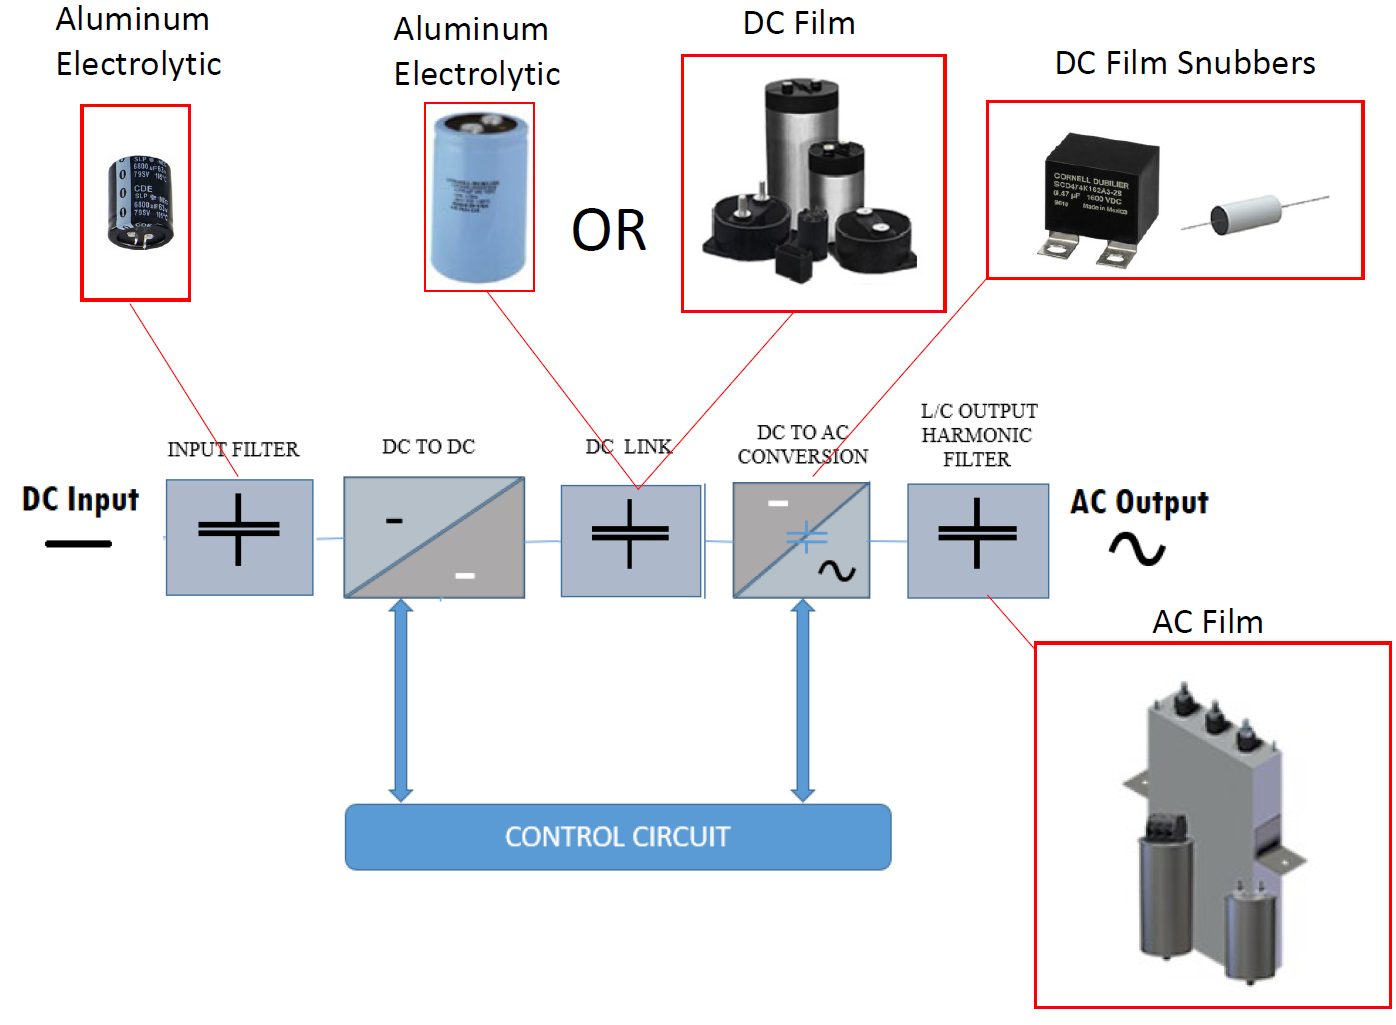
\includegraphics[width=\linewidth]{fig/lec08/capacitors_types.png}
    \caption{Typical capacitor locations in inverter and converter systems: input filter, DC-link, snubber, and AC harmonic filter capacitors. Adapted from Cornell Dubilier, \textit{Capacitors for High Power Inverters and Converters}}
\end{figure}
\end{column}
\end{columns}

\end{frame}


%%%%%%%%%%%%%%%%%%%%%%%%%%%%%%%%%%%%%%%%%%%%%%%%%%%%%%%%%%%%%
%% Capacitors in converter system examples
%%%%%%%%%%%%%%%%%%%%%%%%%%%%%%%%%%%%%%%%%%%%%%%%%%%%%%%%%%%%%
\begin{frame}
\frametitle{Capacitors in Practical Converter Systems}

\begin{columns}
\begin{column}{0.56\textwidth}
The same capacitor principles appear repeatedly in different converter systems.
\begin{itemize}
    \item \textbf{Fast DC EV charger:}
    \begin{itemize}
        \item AC input filter capacitor,
        \item DC-link capacitor,
        \item DC output filter capacitor.
    \end{itemize}

    \item \textbf{Solar inverter:}
    \begin{itemize}
        \item PV-side input filter,
        \item DC-link energy buffer,
        \item AC-side harmonic filter.
    \end{itemize}

    \item \textbf{UPS and VFD systems:}
    \begin{itemize}
        \item rectifier-side filtering,
        \item intermediate DC-link storage,
        \item inverter output filtering.
    \end{itemize}
\end{itemize}
\end{column}

\begin{column}{0.40\textwidth}
\begin{figure}
    \centering
    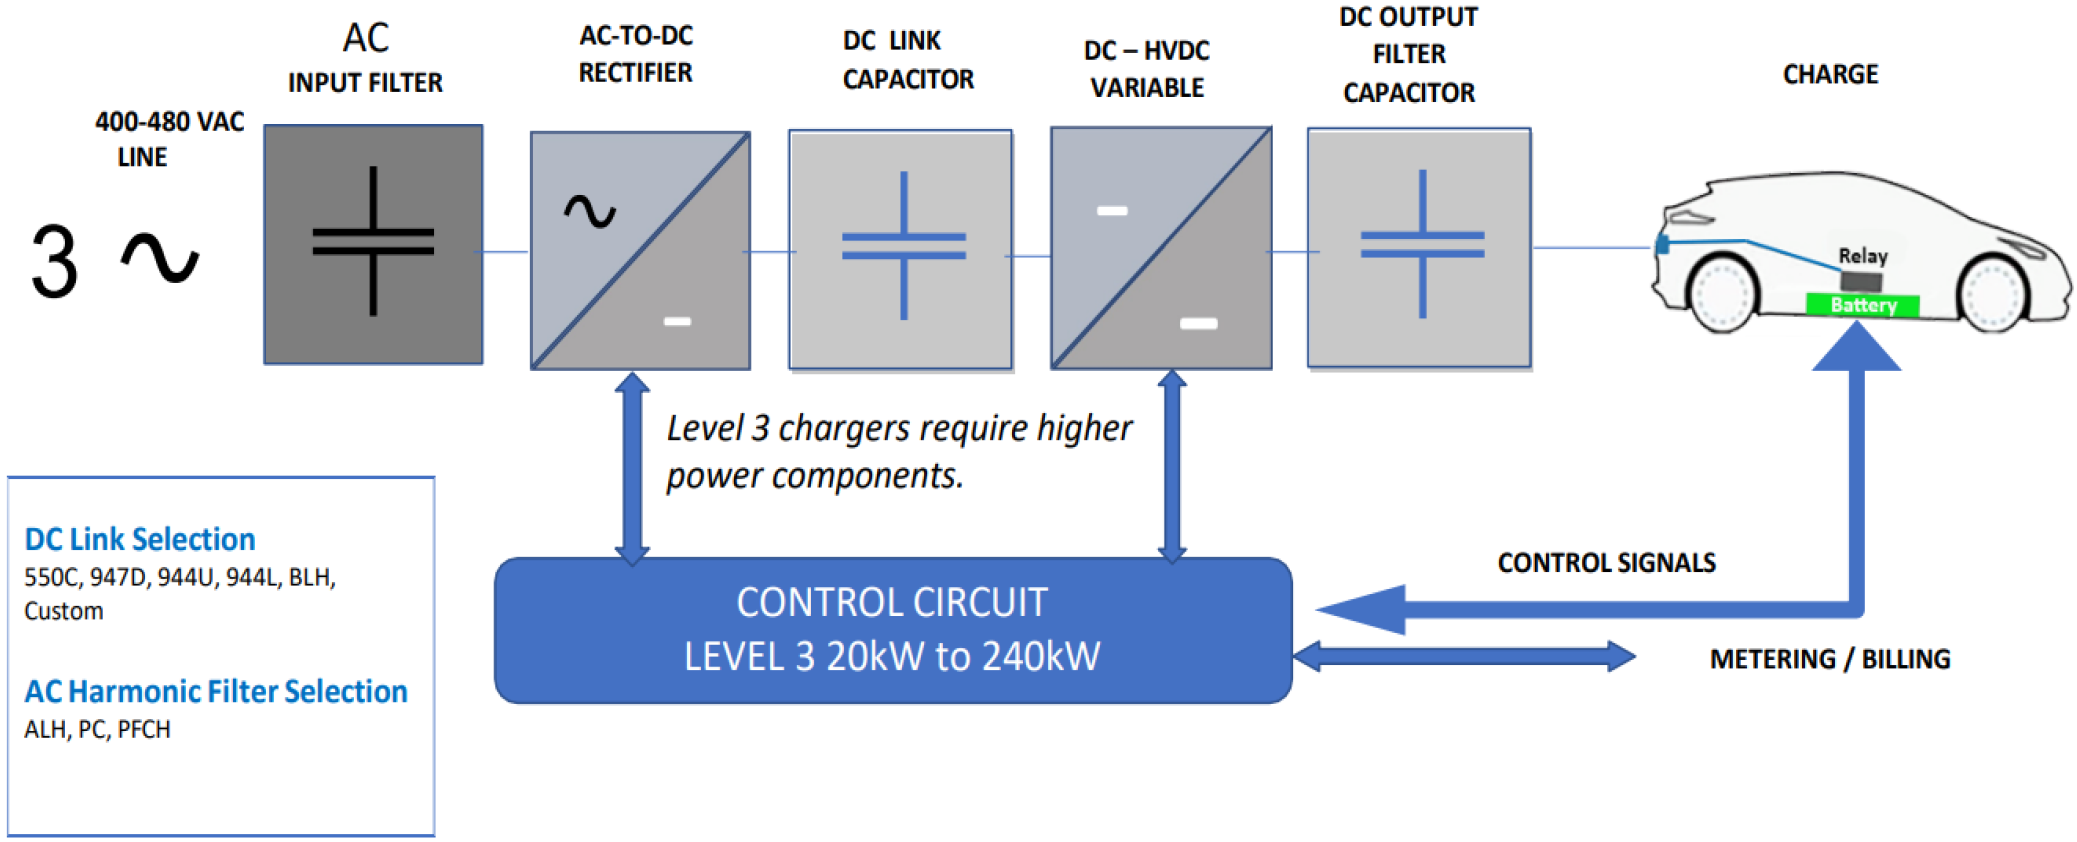
\includegraphics[width=\linewidth]{fig/lec08/fast_dc_ev_charger.png}
    \caption{Capacitor positions in a level-3 fast DC EV charger. Adapted from Cornell Dubilier, \textit{Capacitors for High Power Inverters and Converters}}
\end{figure}
\end{column}
\end{columns}
The capacitor technology changes with the location: electrolytic or film for energy storage, film for DC-link and snubber duties, and ceramics for high-frequency decoupling.
\end{frame}


%%%%%%%%%%%%%%%%%%%%%%%%%%%%%%%%%%%%%%%%%%%%%%%%%%%%%%%%%%%%%
%% Capacitor vs inductor
%%%%%%%%%%%%%%%%%%%%%%%%%%%%%%%%%%%%%%%%%%%%%%%%%%%%%%%%%%%%%
\begin{frame}
\frametitle{Capacitor versus Inductor: Electric-Field and Magnetic-Field Storage}

\begin{columns}
\begin{column}{0.55\textwidth}
A capacitor is the electrical dual of an inductor.
\begin{itemize}
    \item An inductor stores energy in a \textbf{magnetic field}.
    \item A capacitor stores energy in an \textbf{electric field}.
    \item An inductor resists a change in current:
    \begin{align}
        v_L = L\frac{di_L}{dt}
    \end{align}
    \item A capacitor resists a change in voltage:
    \begin{align}
        i_C = C\frac{dv_C}{dt}
    \end{align}
\end{itemize}
This is why inductors smooth current, whereas capacitors smooth voltage.
\end{column}

\begin{column}{0.41\textwidth}
\begin{center}
\begin{circuitikz}[scale=0.85, transform shape]
    \draw (0,0) to[L,l=$L$] (2,0);
    \node at (1,-0.7) {\small magnetic-field storage};
    \draw[->, thick] (-0.2,0.35) -- (0.5,0.35);
    \node at (0.2,0.65) {\small $i_L$};

    \draw (0,-2.0) to[C,l=$C$] (2,-2.0);
    \node at (1,-2.7) {\small electric-field storage};
    \draw[->, thick] (-0.2,-1.65) -- (0.5,-1.65);
    \node at (0.2,-1.35) {\small $i_C$};
\end{circuitikz}
\end{center}

\vspace{0.15cm}

\begin{block}{Power Electronics Interpretation}
\small
The inductor controls the current trajectory; the capacitor controls the voltage trajectory. Converter dynamics are largely shaped by the interaction of both.
\end{block}
\end{column}
\end{columns}

\end{frame}


%%%%%%%%%%%%%%%%%%%%%%%%%%%%%%%%%%%%%%%%%%%%%%%%%%%%%%%%%%%%%
%% Capacitor design questions
%%%%%%%%%%%%%%%%%%%%%%%%%%%%%%%%%%%%%%%%%%%%%%%%%%%%%%%%%%%%%
\begin{frame}
\frametitle{Capacitor Design Questions}
Before selecting a capacitor, the designer must identify the electrical, thermal, mechanical, and reliability requirements.
\begin{columns}
\begin{column}{0.56\textwidth}
\begin{itemize}
    \item What is the required capacitance?
    \item What is the maximum DC voltage?
    \item What ripple voltage is allowed?
    \item What RMS ripple current flows through the capacitor?
    \item What peak current or $dv/dt$ stress occurs during switching?
    \item What ESR and ESL are acceptable?
    \item What temperature rise is acceptable?
    \item What lifetime is required?
    \item Is the capacitor used for DC-link, snubber, EMI, resonant, or output filtering?
\end{itemize}

\end{column}

\begin{column}{0.40\textwidth}
\begin{block}{Selection Principle}
\small
A capacitor is not selected by capacitance alone. In power electronics, the correct capacitor is selected by a combined requirement:
\[
V,\; C,\; I_{\mathrm{rms}},\; I_{\mathrm{pk}},\; ESR,\; ESL,\; T,\; L_{\mathrm{life}}
\]
\end{block}

\begin{block}{Practical Source}
\small
The selection guide for capacitors should be structured based on voltage, capacitance, current withstand, and power-loss/temperature-rise checks.
\end{block}
\end{column}
\end{columns}

\end{frame}


%%%%%%%%%%%%%%%%%%%%%%%%%%%%%%%%%%%%%%%%%%%%%%%%%%%%%%%%%%%%%
%% Capacitance definition
%%%%%%%%%%%%%%%%%%%%%%%%%%%%%%%%%%%%%%%%%%%%%%%%%%%%%%%%%%%%%
\begin{frame}
\frametitle{Capacitance: Ability to Store Electric Charge}

\begin{columns}
\begin{column}{0.55\textwidth}
Capacitance describes how much electric charge is stored per unit voltage $C = \frac{Q}{V}$, where
\begin{itemize}
    \item $C$ is capacitance in farads,
    \item $Q$ is stored charge in coulombs,
    \item $V$ is voltage across the capacitor.
\end{itemize}
The current through a capacitor follows from differentiating charge:
\begin{align}
    i_C(t) = \frac{dQ}{dt}
           = C\frac{dv_C(t)}{dt}
\end{align}
Therefore, a capacitor conducts current only when its voltage changes. Under ideal steady-state DC conditions, capacitor current becomes zero.
\end{column}

\begin{column}{0.41\textwidth}
\begin{figure}
    \centering
    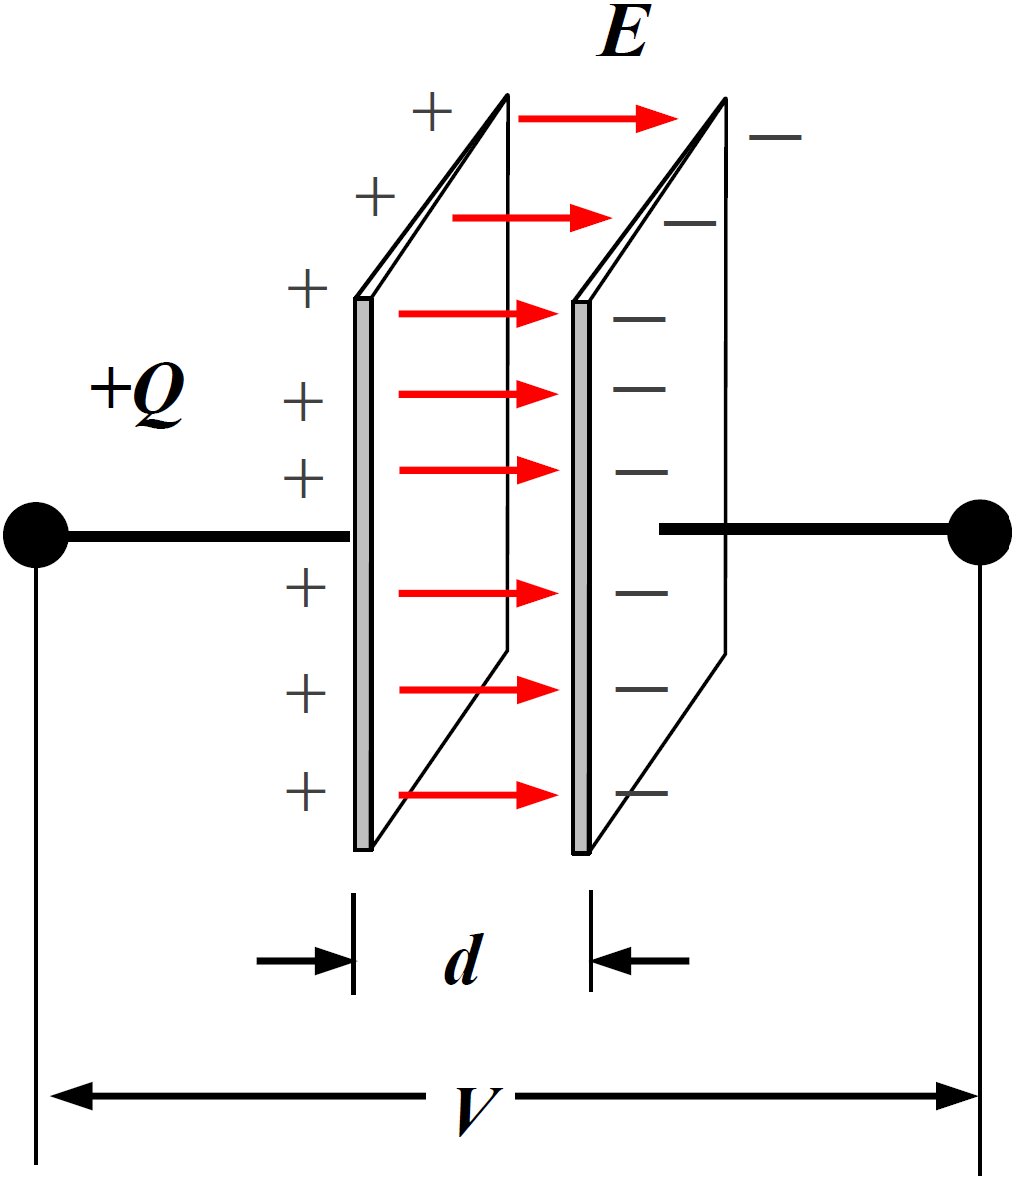
\includegraphics[width=0.6\linewidth]{fig/lec08/charge_and_electric_field.png}
    \caption{Electric charge and electric field strength between capacitor plates. Adapted from AIC tech, \textit{The Three Essential Characteristics of Capacitors}}
\end{figure}
\end{column}
\end{columns}

\end{frame}


%%%%%%%%%%%%%%%%%%%%%%%%%%%%%%%%%%%%%%%%%%%%%%%%%%%%%%%%%%%%%
%% Parallel plate capacitor
%%%%%%%%%%%%%%%%%%%%%%%%%%%%%%%%%%%%%%%%%%%%%%%%%%%%%%%%%%%%%
\begin{frame}
\frametitle{Parallel-Plate Capacitor}

\begin{columns}
\begin{column}{0.55\textwidth}
For an ideal parallel-plate capacitor,
\begin{align}
    C = \varepsilon_0\varepsilon_r \frac{A}{d}
\end{align}
where
\begin{itemize}
    \item $\varepsilon_0$ is the permittivity of free space,
    \item $\varepsilon_r$ is the relative permittivity of the dielectric,
    \item $A$ is the electrode area,
    \item $d$ is the dielectric thickness.
\end{itemize}
Hence three main ways to increase capacitance:
\begin{itemize}
    \item increase electrode area,
    \item use a dielectric with higher $\varepsilon_r$,
    \item reduce dielectric thickness.
\end{itemize}
\end{column}

\begin{column}{0.41\textwidth}
\begin{figure}
    \centering
    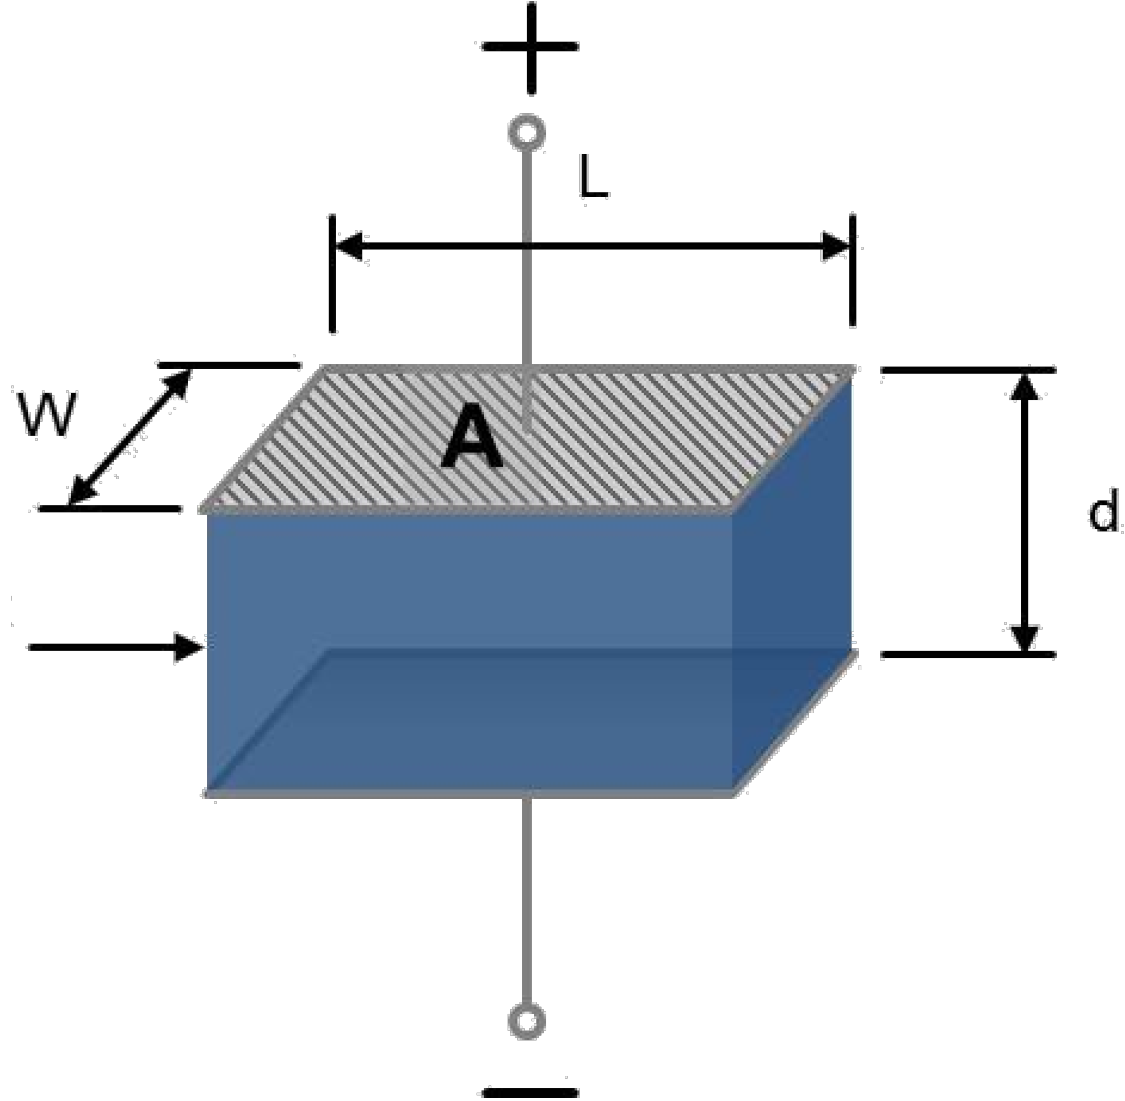
\includegraphics[width=0.6\linewidth]{fig/lec08/plate_capacitor.png}
    \caption{Construction of a plate capacitor and the relation $C=\varepsilon_0\varepsilon_r A/d$. Adapted from W{\"u}rth Elektronik, \textit{Fundamentals of Capacitor Technology and Their Applications}}
\end{figure}
\end{column}
\end{columns}
However, reducing $d$ increases the electric field stress and reduces voltage withstand capability.
\end{frame}


%%%%%%%%%%%%%%%%%%%%%%%%%%%%%%%%%%%%%%%%%%%%%%%%%%%%%%%%%%%%%
%% Electric field and dielectric stress
%%%%%%%%%%%%%%%%%%%%%%%%%%%%%%%%%%%%%%%%%%%%%%%%%%%%%%%%%%%%%
\begin{frame}
\frametitle{Electric Field and Dielectric Stress}

\begin{columns}
\begin{column}{0.56\textwidth}
The electric field inside a parallel-plate capacitor is approximately $E = \frac{V}{d}$, where $V$ is the applied voltage and $d$ is the dielectric thickness. This simple equation is extremely important for power electronics:
\begin{itemize}
    \item Higher voltage increases dielectric stress.
    \item Thinner dielectric increases capacitance but also increases electric field.
    \item Exceeding the dielectric strength causes partial discharge, insulation degradation, or breakdown.
    \item Voltage derating is therefore essential for long lifetime.
\end{itemize}
\end{column}

\begin{column}{0.40\textwidth}
    \vspace{-0.75cm}
\begin{block}{Design Interpretation}
The capacitance equation encourages small dielectric thickness, but the electric-field equation limits how small the dielectric can be:
\[
C \uparrow \quad \text{when} \quad d \downarrow
\]
\[
E \uparrow \quad \text{when} \quad d \downarrow
\]
\end{block}
\begin{block}{Practical Consequence}
Capacitor design is a compromise between capacitance density, voltage rating, loss, reliability, and lifetime.
\end{block}
\end{column}
\end{columns}
In real capacitors, field enhancement also occurs near electrode edges, metallization boundaries, terminals, and defects.
\end{frame}


%%%%%%%%%%%%%%%%%%%%%%%%%%%%%%%%%%%%%%%%%%%%%%%%%%%%%%%%%%%%%
%% Dielectric polarization
%%%%%%%%%%%%%%%%%%%%%%%%%%%%%%%%%%%%%%%%%%%%%%%%%%%%%%%%%%%%%
\begin{frame}
\frametitle{Dielectric Polarization}

\begin{columns}
\begin{column}{0.55\textwidth}
A dielectric is an insulating material that becomes polarized when exposed to an electric field.
When the dielectric is inserted between the plates:
\begin{itemize}
    \item bound charges shift slightly inside the material,
    \item an induced electric field is created,
    \item the net electric field for a given charge is reduced,
    \item more charge can be stored at the same applied voltage.
\end{itemize}
The capacitance therefore increases by the relative permittivity:
\begin{align}
    C = \varepsilon_r C_0
\end{align}
where $C_0$ is the capacitance without the dielectric.
\end{column}

\begin{column}{0.41\textwidth}
\begin{figure}
    \centering
    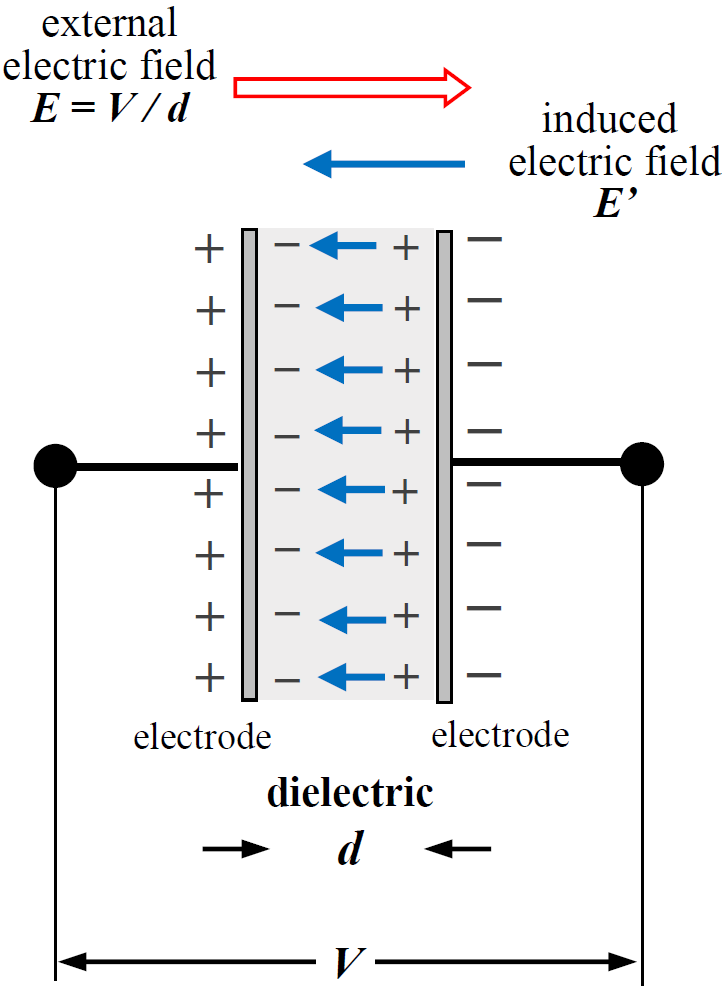
\includegraphics[width=0.5\linewidth]{fig/lec08/dielectric_polarization.png}
    \caption{Dielectric polarization caused by an applied electric field. Adapted from AIC tech, \textit{The Three Essential Characteristics of Capacitors}}
\end{figure}
\end{column}
\end{columns}
Different capacitor technologies are largely distinguished by their dielectric material.
\end{frame}


%%%%%%%%%%%%%%%%%%%%%%%%%%%%%%%%%%%%%%%%%%%%%%%%%%%%%%%%%%%%%
%% Dielectric materials
%%%%%%%%%%%%%%%%%%%%%%%%%%%%%%%%%%%%%%%%%%%%%%%%%%%%%%%%%%%%%
\begin{frame}
\frametitle{Dielectric Materials and Relative Permittivity}

\begin{columns}
\begin{column}{0.56\textwidth}
The dielectric determines capacitance density, loss, temperature stability, voltage dependence, and ageing. Typical examples:
\begin{itemize}
    \item \textbf{Polypropylene:} low loss, stable, widely used in film capacitors.
    \item \textbf{Aluminum oxide:} dielectric of aluminum electrolytic capacitors.
    \item \textbf{Tantalum oxide:} used in tantalum electrolytic capacitors.
    \item \textbf{Class 1 ceramics:} stable, low loss, lower capacitance.
    \item \textbf{Class 2 ceramics:} high capacitance, but voltage- and temperature-dependent.
\end{itemize}

\end{column}

\begin{column}{0.40\textwidth}
\begin{figure}
    \centering
    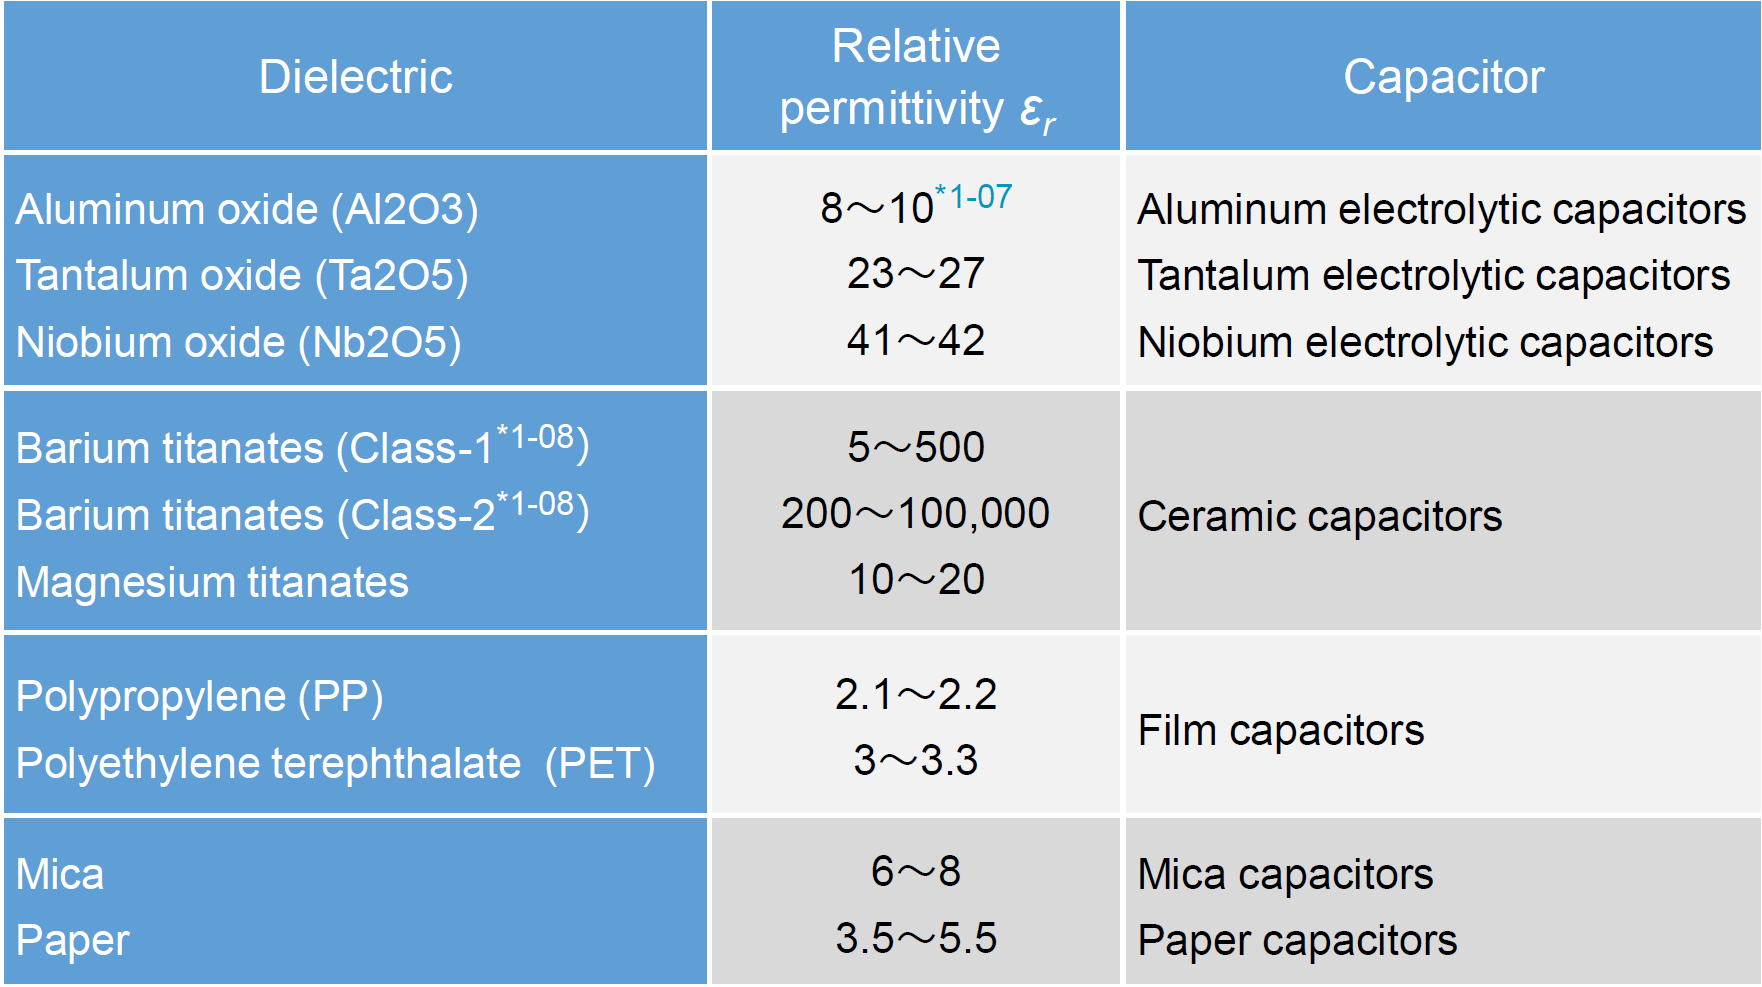
\includegraphics[width=\linewidth]{fig/lec08/dielectrics.png}
    \caption{Dielectric types, relative permittivity, and corresponding capacitor families. Adapted from AIC tech, \textit{The Three Essential Characteristics of Capacitors}}
\end{figure}
\end{column}
\end{columns}
High $\varepsilon_r$ gives high capacitance density, but not necessarily the best power-electronics capacitor. Loss, voltage dependence, ripple current, and thermal behaviour must also be considered.
\end{frame}


%%%%%%%%%%%%%%%%%%%%%%%%%%%%%%%%%%%%%%%%%%%%%%%%%%%%%%%%%%%%%
%% Stored energy
%%%%%%%%%%%%%%%%%%%%%%%%%%%%%%%%%%%%%%%%%%%%%%%%%%%%%%%%%%%%%
\begin{frame}
\frametitle{Energy Stored in a Capacitor}

\begin{columns}
\begin{column}{0.56\textwidth}
The energy stored in a capacitor is
\begin{align}
    E_C = \int_0^Q v\,dq
\end{align}
\begin{align}
    E_C = \frac{1}{2}CV^2 [\text{using} q = Cv]
\end{align}
Important observations:
\begin{itemize}
    \item Stored energy increases linearly with capacitance.
    \item Stored energy increases with the square of voltage.
    \item High-voltage DC-link capacitors can store dangerous energy even after the converter is switched off.
    \item Discharge resistors and safe handling procedures are therefore essential.
\end{itemize}

\end{column}

\begin{column}{0.40\textwidth}
\begin{figure}
    \centering
    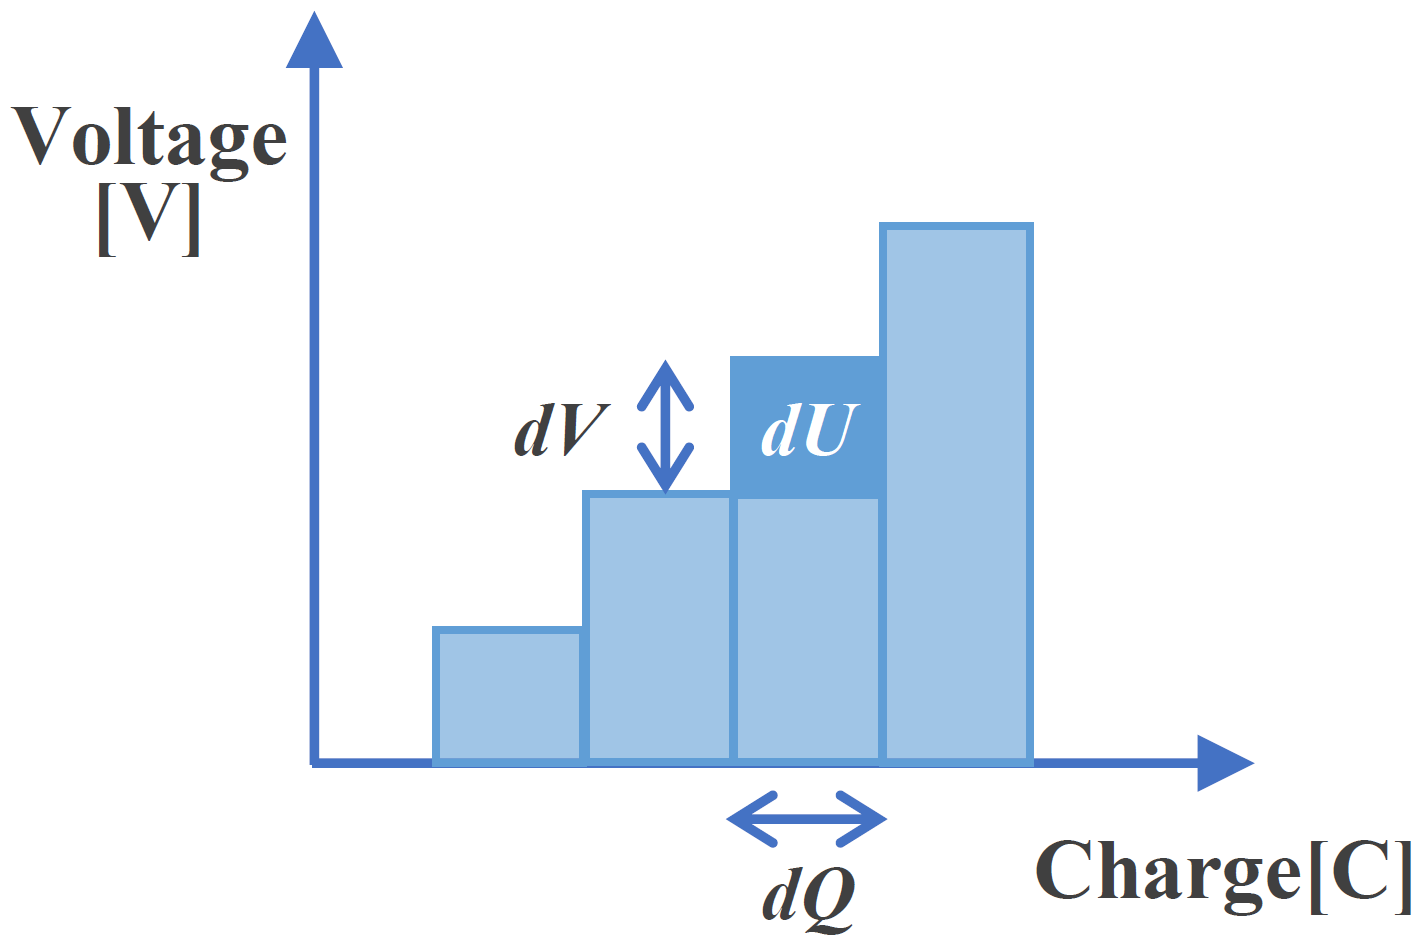
\includegraphics[width=0.5\linewidth]{fig/lec08/cap_energy_storage.png}
    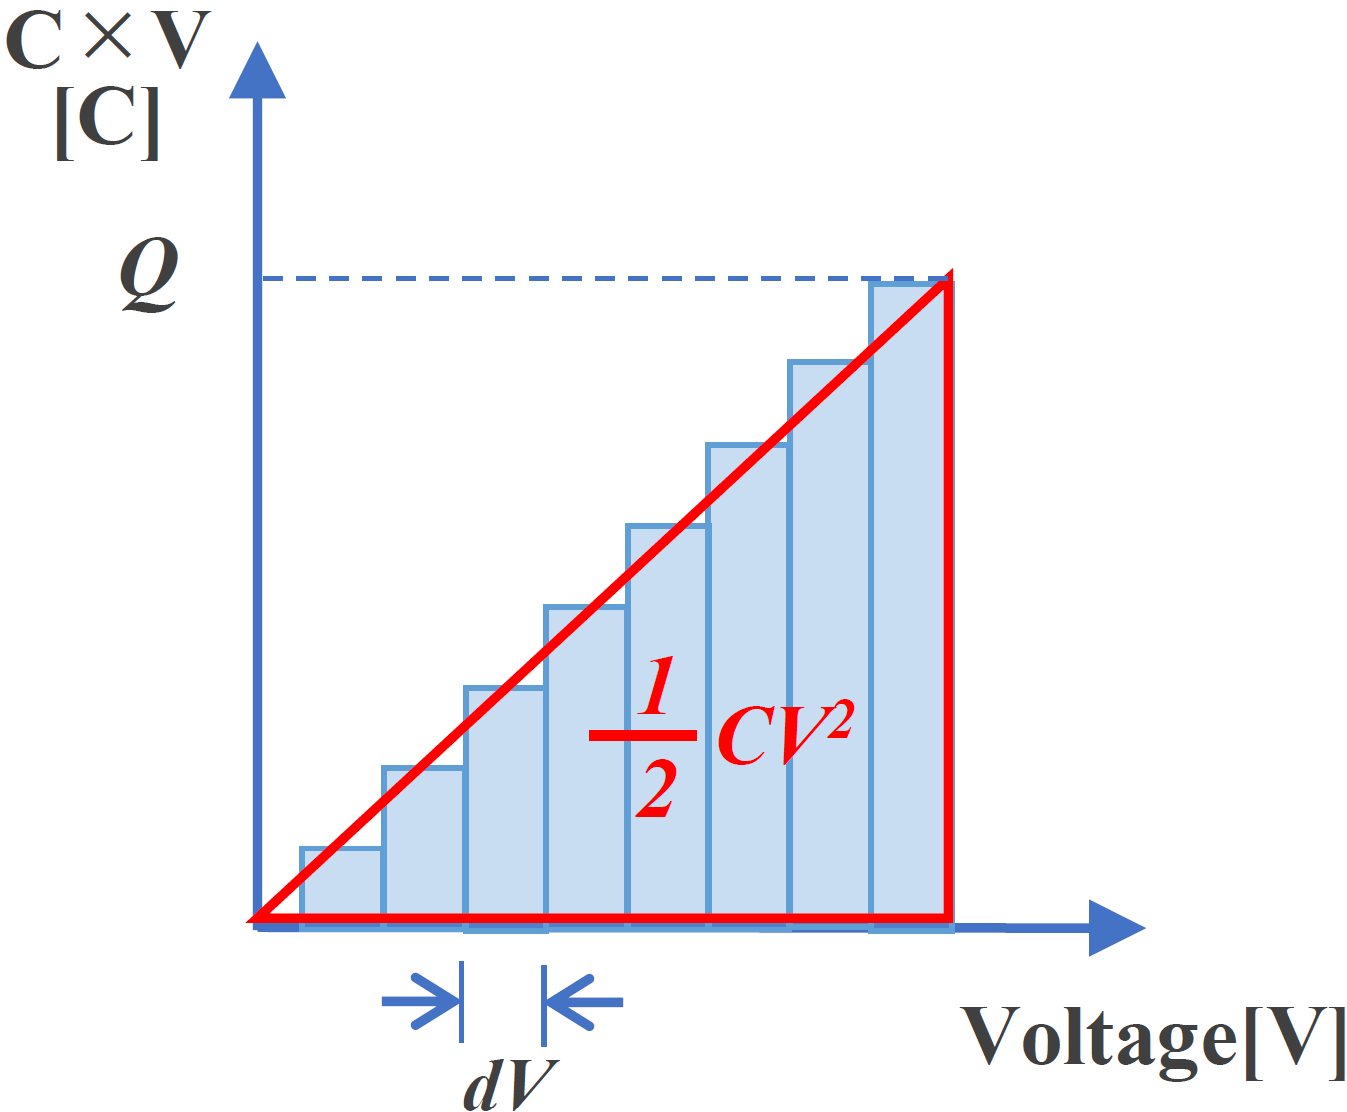
\includegraphics[width=0.5\linewidth]{fig/lec08/cap_energy_storage2.png}
    \caption{Charge--voltage relation and stored energy in a capacitor. Adapted from AIC tech, \textit{The Three Essential Characteristics of Capacitors}}
\end{figure}
\end{column}
\end{columns}
\end{frame}


%%%%%%%%%%%%%%%%%%%%%%%%%%%%%%%%%%%%%%%%%%%%%%%%%%%%%%%%%%%%%
%% Capacitor current and dvdt
%%%%%%%%%%%%%%%%%%%%%%%%%%%%%%%%%%%%%%%%%%%%%%%%%%%%%%%%%%%%%
\begin{frame}
\frametitle{Capacitor Current and $dv/dt$ Stress}

\begin{columns}
\begin{column}{0.55\textwidth}
The capacitor current is $i_C(t)=C\frac{dv_C(t)}{dt}$. This equation is central in switched-mode power converters.
\begin{itemize}
    \item A slowly varying voltage produces small capacitor current.
    \item A fast switching edge produces large current.
    \item High $dv/dt$ creates high peak current stress.
    \item In snubbers and DC-link decoupling, the capacitor must withstand repetitive high-current pulses.
\end{itemize}
For a linear voltage transition,
\begin{align}
    I_{\mathrm{pk}} = C\frac{\Delta V}{\Delta t}
\end{align}
\end{column}

\begin{column}{0.41\textwidth}
\begin{center}
\begin{circuitikz}[scale=0.80, transform shape]
    \draw (0,0) to[C,l=$C$] (0,-2);
    \draw (-1,0) -- (1,0);
    \draw (-1,-2) -- (1,-2);
    \draw[->, thick] (1.2,-1.7) -- (1.2,-0.3);
    \node at (1.55,-1.0) {$i_C$};

    \draw[->] (-0.6,-2.6) -- (2.8,-2.6);
    \draw[->] (-0.6,-2.6) -- (-0.6,-0.6);
    \draw[thick] (-0.4,-2.4) -- (0.5,-2.4) -- (2.1,-1.0) -- (2.6,-1.0);
    \node at (2.65,-2.75) {\small $t$};
    \node at (-0.95,-0.8) {\small $v_C$};
    \node at (1.3,-1.9) {\small $\Delta V/\Delta t$};
\end{circuitikz}
\end{center}

\begin{block}{Power Electronics Interpretation}
\small
Fast SiC/GaN switching increases $dv/dt$, so the capacitor must be evaluated for peak current, RMS current, ESL, mounting inductance, and thermal stress.
\end{block}
\end{column}
\end{columns}
Thus, increasing capacitance or reducing rise time increases pulse current.
\end{frame}


%%%%%%%%%%%%%%%%%%%%%%%%%%%%%%%%%%%%%%%%%%%%%%%%%%%%%%%%%%%%%
%% Charging and discharging
%%%%%%%%%%%%%%%%%%%%%%%%%%%%%%%%%%%%%%%%%%%%%%%%%%%%%%%%%%%%%
\begin{frame}
\frametitle{Charging and Discharging of a Capacitor}

\begin{columns}
\begin{column}{0.65\textwidth}
In RC charging circuit, the capacitor voltage rises exponentially:
\begin{align}
    v_C(t)=V\left(1-e^{-t/RC}\right)
\end{align}
The charging current is
\begin{align}
    i_C(t)=\frac{V}{R}e^{-t/RC}
\end{align}
The time constant is $\tau = RC$. In power electronics, this principle appears in:
\begin{itemize}
    \item DC-link pre-charge circuits,
    \item discharge resistors,
    \item soft-start circuits,
    \item hold-up time design, and safety after shutdown.
\end{itemize}
\end{column}

\begin{column}{0.35\textwidth}
\begin{figure}
    \centering
    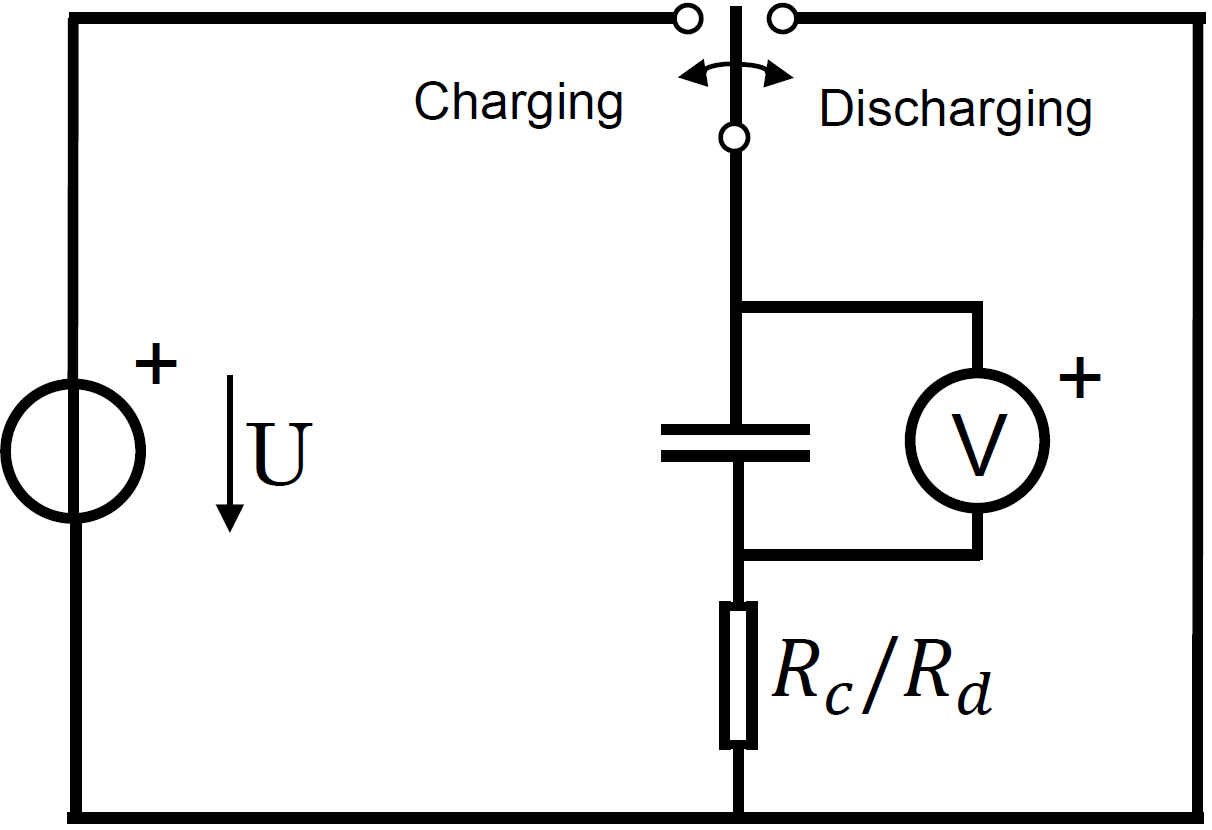
\includegraphics[width=0.8\linewidth]{fig/lec08/charging_discharging.png}
    \caption{Charging and discharging waveforms of a capacitor with time constant $\tau=RC$. Adapted from W{\"u}rth Elektronik, \textit{Fundamentals of Capacitor Technology and Their Applications}}
\end{figure}
\end{column}
\end{columns}

\end{frame}


%%%%%%%%%%%%%%%%%%%%%%%%%%%%%%%%%%%%%%%%%%%%%%%%%%%%%%%%%%%%%
%% Capacitive reactance
%%%%%%%%%%%%%%%%%%%%%%%%%%%%%%%%%%%%%%%%%%%%%%%%%%%%%%%%%%%%%
\begin{frame}
\frametitle{Capacitor in AC Circuits: Capacitive Reactance}
\begin{columns}
\begin{column}{0.56\textwidth}
For sinusoidal excitation, the impedance of an ideal capacitor is $Z_C = \frac{1}{j\omega C}$, and the capacitive reactance magnitude is
\begin{align}
    X_C = \frac{1}{\omega C}
        = \frac{1}{2\pi f C}
\end{align}
Therefore:
\begin{itemize}
    \item at low frequency, $X_C$ is large,
    \item at high frequency, $X_C$ becomes small,
    \item capacitor current leads capacitor voltage by $90^\circ$ in the ideal case,
    \item capacitors can be used for filtering, bypassing, coupling, and resonance.
\end{itemize}
\end{column}

\begin{column}{0.40\textwidth}
\begin{center}
\begin{circuitikz}[scale=0.80, transform shape]
    \draw (0,0) to[sV,l=$v_C$] (0,-2)
          to[C,l=$C$] (2,-2)
          -- (2,0) -- (0,0);

    \draw[->, thick] (3.0,-1.2) -- (4.2,-1.2);
    \node at (4.4,-1.2) {$V_C$};

    \draw[->, thick] (3.0,-1.2) -- (3.0,0.0);
    \node at (3.0,0.25) {$I_C$};

    \node at (3.75,-0.5) {\small $I_C$ leads $V_C$};
\end{circuitikz}
\end{center}
\begin{block}{Design Message}
\small
Capacitors are selected by their impedance over the relevant frequency range, not only by their nominal capacitance.
\end{block}
\end{column}
\end{columns}
However, real capacitors stop behaving ideally at high frequency due to ESR and ESL.
\end{frame}


%%%%%%%%%%%%%%%%%%%%%%%%%%%%%%%%%%%%%%%%%%%%%%%%%%%%%%%%%%%%%
%% Ideal capacitor summary
%%%%%%%%%%%%%%%%%%%%%%%%%%%%%%%%%%%%%%%%%%%%%%%%%%%%%%%%%%%%%
\begin{frame}
\frametitle{Summary of Ideal Capacitor Behaviour}
\begin{itemize}
    \item A capacitor stores electric charge according to $Q=CV$.
    \item The capacitance of an ideal parallel-plate capacitor is
    \begin{align}
        C=\varepsilon_0\varepsilon_r\frac{A}{d}
    \end{align}
    \item The electric field stress is approximately
    \begin{align}
        E=\frac{V}{d}
    \end{align}
    \item The capacitor current is proportional to voltage slew rate:
    \begin{align}
        i_C=C\frac{dv_C}{dt}
    \end{align}
    \item The stored energy is
    \begin{align}
        E_C=\frac{1}{2}CV^2
    \end{align}
    \item In DC steady state, an ideal capacitor behaves as an open circuit.
    \item In AC and switching circuits, it provides a frequency-dependent current path.
\end{itemize}
\end{frame}


%%%%%%%%%%%%%%%%%%%%%%%%%%%%%%%%%%%%%%%%%%%%%%%%%%%%%%%%%%%%%
%% Why ideal capacitor model is not enough
%%%%%%%%%%%%%%%%%%%%%%%%%%%%%%%%%%%%%%%%%%%%%%%%%%%%%%%%%%%%%
\begin{frame}
\frametitle{Why is the Ideal Capacitor Model Not Enough?}
The ideal capacitor relation $i_C = C\frac{dv_C}{dt}$ is useful for understanding the basic function of a capacitor. However, it is not sufficient for practical power electronic converter design. A real capacitor also contains parasitic and loss elements:

\begin{itemize}
    \item \textbf{Equivalent series resistance (ESR):} produces heat under ripple current.
    \item \textbf{Equivalent series inductance (ESL):} causes high-frequency impedance rise and voltage spikes.
    \item \textbf{Leakage resistance:} allows a small DC current through the dielectric.
    \item \textbf{Dielectric loss:} produces additional AC loss, usually represented by $\tan\delta$.
    \item \textbf{Dielectric absorption:} causes residual or recovery voltage after discharge.
\end{itemize}

Therefore, in power electronics, a capacitor must be treated as a frequency-dependent impedance rather than as a fixed capacitance.

\end{frame}


%%%%%%%%%%%%%%%%%%%%%%%%%%%%%%%%%%%%%%%%%%%%%%%%%%%%%%%%%%%%%
%% Real capacitor equivalent circuit
%%%%%%%%%%%%%%%%%%%%%%%%%%%%%%%%%%%%%%%%%%%%%%%%%%%%%%%%%%%%%
\begin{frame}
\frametitle{Equivalent Circuit of a Real Capacitor}

\begin{columns}
\begin{column}{0.55\textwidth}
A practical capacitor can be represented by an ideal capacitance combined with parasitic resistance, inductance, and leakage paths.
\begin{itemize}
    \item $C$ represents the useful capacitance.
    \item $R_{\mathrm{ESR}}$ represents ohmic and dielectric losses.
    \item $L_{\mathrm{ESL}}$ represents terminal, lead, winding, and layout inductance.
    \item $R_{\mathrm{leak}}$ represents insulation resistance and DC leakage.
\end{itemize}
The simplified impedance is
\begin{align}
    Z(j\omega)
    =
    R_{\mathrm{ESR}}
    +
    j\omega L_{\mathrm{ESL}}
    +
    \frac{1}{j\omega C}
\end{align}
\end{column}
\begin{column}{0.41\textwidth}
\begin{center}
\begin{circuitikz}[scale=0.88, transform shape]
    \draw (0,0) to[L,l=$L_{\mathrm{ESL}}$] (1.7,0)
              to[R,l=$R_{\mathrm{ESR}}$] (3.4,0)
              to[C,l=$C$] (3.4,-2.0)
              -- (0,-2.0) -- (0,0);

    \draw (4.2,0) -- (4.2,-2.0);
    \draw (3.4,0) -- (4.2,0);
    \draw (3.4,-2.0) -- (4.2,-2.0);
    \draw (4.2,0) to[R,l=$R_{\mathrm{leak}}$] (4.2,-2.0);

    \node at (-0.25,-1.0) {$+$};
    \node at (-0.25,-1.35) {$-$};
\end{circuitikz}
\end{center}

\begin{block}{Model Interpretation}
The useful capacitance stores energy, but ESR, ESL, and leakage determine loss, heating, resonance, switching spikes, and long-term reliability.
\end{block}
\end{column}
\end{columns}
This expression already explains why the same capacitor behaves differently at low, medium, and high frequency.
\end{frame}


%%%%%%%%%%%%%%%%%%%%%%%%%%%%%%%%%%%%%%%%%%%%%%%%%%%%%%%%%%%%%
%% ESR
%%%%%%%%%%%%%%%%%%%%%%%%%%%%%%%%%%%%%%%%%%%%%%%%%%%%%%%%%%%%%
\begin{frame}
\frametitle{Equivalent Series Resistance: ESR}

\begin{columns}
\begin{column}{0.56\textwidth}
The equivalent series resistance represents all loss mechanisms that appear as an effective resistance in series with the capacitance. Main contributors include:
\begin{itemize}
    \item electrode resistance,
    \item metallization resistance,
    \item terminal and contact resistance,
    \item electrolyte resistance in electrolytic capacitors,
    \item dielectric losses under AC excitation.
\end{itemize}
The most important consequence of ESR is self-heating:
\begin{align}
    P_{\mathrm{ESR}}
    =
    I_{\mathrm{rms}}^2 R_{\mathrm{ESR}}
\end{align}
\end{column}

\begin{column}{0.40\textwidth}
\begin{figure}
    \centering
    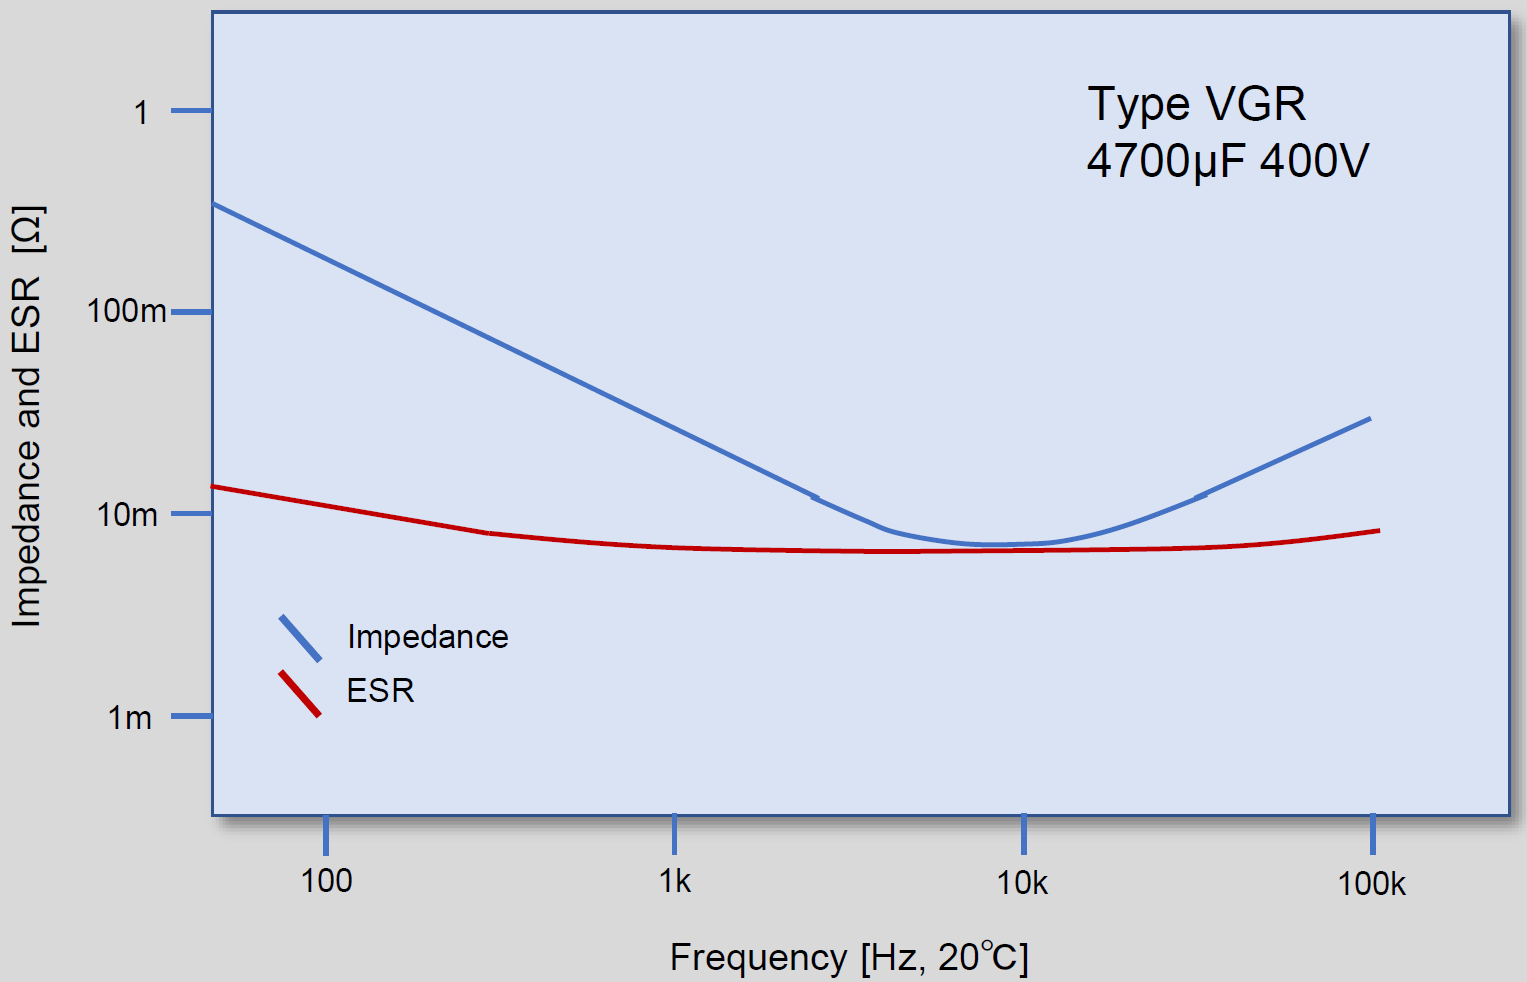
\includegraphics[width=0.8\linewidth]{fig/lec08/impedance_ESR_frequency.png}
    \caption{Impedance and ESR variation with frequency for an aluminum electrolytic capacitor. Adapted from AIC tech, \textit{The Three Essential Characteristics of Capacitors}}
\end{figure}
\end{column}
\end{columns}
A capacitor carrying high ripple current can fail thermally even when its voltage and capacitance ratings appear correct.
\end{frame}


%%%%%%%%%%%%%%%%%%%%%%%%%%%%%%%%%%%%%%%%%%%%%%%%%%%%%%%%%%%%%
%% ESR design implication
%%%%%%%%%%%%%%%%%%%%%%%%%%%%%%%%%%%%%%%%%%%%%%%%%%%%%%%%%%%%%
\begin{frame}
\frametitle{ESR: Design Consequences}
\begin{columns}
\begin{column}{0.5\textwidth}
ESR is critical in converter capacitors: it sets ripple voltage, loss, and lifetime. For a ripple current component,
\begin{align}
    \Delta v_{\mathrm{ESR}}
    =
    i_C R_{\mathrm{ESR}}
\end{align}
and the thermal loss is
\begin{align}
    P_{\mathrm{loss}}
    =
    I_{\mathrm{C,rms}}^2R_{\mathrm{ESR}}
\end{align}
High ESR causes:
\begin{itemize}
    \item larger ripple voltage,
    \item increased internal hot-spot temperature,
    \item accelerated ageing,
    \item reduced ripple-current capability,
    \item possible thermal runaway in severe cases.
\end{itemize}
\end{column}

\begin{column}{0.48\textwidth}
\begin{block}{Power Electronics Interpretation}
\small
In a DC-link or output capacitor, the RMS current rating is often more restrictive than the capacitance rating. A larger capacitance value does not automatically mean a better capacitor if ESR and thermal resistance are poor.
\end{block}
\begin{block}{Practical Check}
\small
Always check:
\[
I_{\mathrm{C,rms}} < I_{\mathrm{rated,rms}}
\]
at the expected operating temperature and cooling condition.
\end{block}
\end{column}
\end{columns}

\end{frame}


%%%%%%%%%%%%%%%%%%%%%%%%%%%%%%%%%%%%%%%%%%%%%%%%%%%%%%%%%%%%%
%% ESL
%%%%%%%%%%%%%%%%%%%%%%%%%%%%%%%%%%%%%%%%%%%%%%%%%%%%%%%%%%%%%
\begin{frame}
\frametitle{Equivalent Series Inductance: ESL}

\begin{columns}
\begin{column}{0.56\textwidth}
The equivalent series inductance is caused by the current path through terminals, leads, internal electrodes, tabs, windings, busbars, and PCB layout. At high frequency, $X_L = \omega L_{\mathrm{ESL}}$ becomes significant. ESL causes:
\begin{itemize}
    \item impedance increase above self-resonance,
    \item voltage overshoot during fast current commutation,
    \item reduced high-frequency decoupling effectiveness,
    \item increased switching-loop ringing,
    \item EMI problems in SiC and GaN converters.
\end{itemize}
The voltage generated by ESL is
\begin{align}
    v_{\mathrm{ESL}} = L_{\mathrm{ESL}}\frac{di}{dt}
\end{align}
\end{column}

\begin{column}{0.40\textwidth}
\begin{figure}
    \centering
    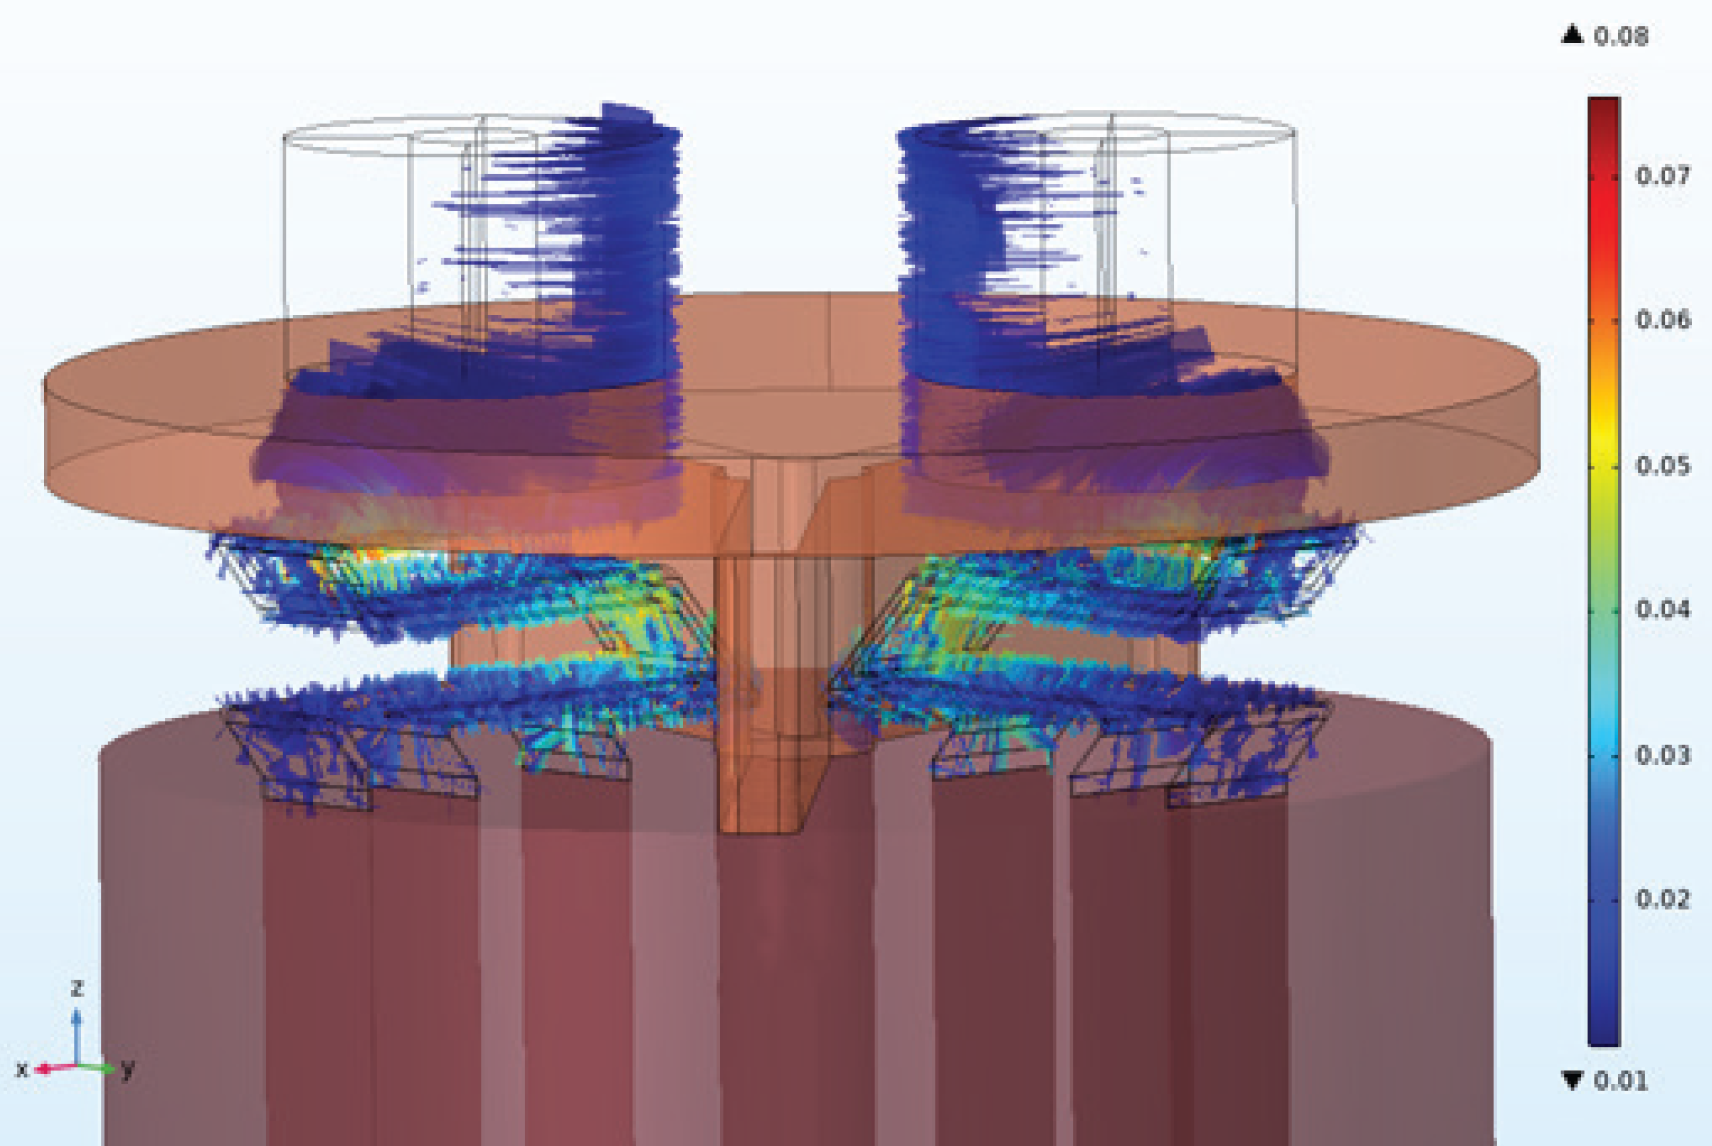
\includegraphics[width=0.8\linewidth]{fig/lec08/flux_lines_terminal_inductance.png}
    \caption{Typical magnetic flux lines in a screw-terminal capacitor with ripple current, illustrating terminal and tab loop inductance. Adapted from Knowles/Cornell Dubilier, \textit{Aluminum Electrolytic Capacitor Application Guide}}
\end{figure}
\end{column}
\end{columns}

\end{frame}


%%%%%%%%%%%%%%%%%%%%%%%%%%%%%%%%%%%%%%%%%%%%%%%%%%%%%%%%%%%%%
%% ESL and switching spikes
%%%%%%%%%%%%%%%%%%%%%%%%%%%%%%%%%%%%%%%%%%%%%%%%%%%%%%%%%%%%%
\begin{frame}
\frametitle{ESL and Switching Voltage Spikes}

\begin{columns}
\begin{column}{0.55\textwidth}
In fast-switching converters, the capacitor current can change within a few nanoseconds. The parasitic inductive voltage becomes
\begin{align}
    v_{\mathrm{spike}}
    =
    L_{\mathrm{loop}}
    \frac{di}{dt}
\end{align}
with $L_{\mathrm{loop}} =$ capacitor ESL + layout inductance. In SiC/GaN converters:
\begin{itemize}
    \item high $di/dt$,
    \item minimize loop area,
    \item use compact PCB loops or laminated busbars,
    \item add local HF ceramic/power-ceramic capacitors.
\end{itemize}
\end{column}

\begin{column}{0.41\textwidth}
\begin{center}
\begin{circuitikz}[scale=0.82, transform shape]
    \draw (0,0) to[V,l=$V_{\mathrm{dc}}$] (0,-2.5);
    \draw (0,0) -- (1.2,0)
          to[L,l=$L_{\mathrm{loop}}$] (2.7,0)
          to[C,l=$C_{\mathrm{dc}}$] (2.7,-2.5)
          -- (0,-2.5);

    \draw (2.7,0) -- (4.2,0)
          to[short] (4.2,-0.8)
          to[closing switch,l=$S$] (4.2,-1.7)
          to[short] (4.2,-2.5)
          -- (2.7,-2.5);

    \draw[->, thick] (1.3,0.45) -- (2.4,0.45);
    \node at (1.85,0.75) {\small $di/dt$};
    \node at (2.0,-3.0) {\small compact DC-link loop};
\end{circuitikz}
\end{center}

\begin{block}{Design Message}
For WBG converters, the capacitor and layout must be designed together. A low-ESL capacitor can still perform poorly if the external loop inductance is large.
\end{block}
\end{column}
\end{columns}

\end{frame}


%%%%%%%%%%%%%%%%%%%%%%%%%%%%%%%%%%%%%%%%%%%%%%%%%%%%%%%%%%%%%
%% Impedance versus frequency
%%%%%%%%%%%%%%%%%%%%%%%%%%%%%%%%%%%%%%%%%%%%%%%%%%%%%%%%%%%%%
\begin{frame}
\frametitle{Impedance versus Frequency}
\begin{columns}
\begin{column}{0.56\textwidth}
For the simplified series RLC capacitor model,
\begin{align}
    Z(j\omega)
    =
    R_{\mathrm{ESR}}
    +
    j\left(
    \omega L_{\mathrm{ESL}}
    -
    \frac{1}{\omega C}
    \right)
\end{align}
The magnitude becomes
\begin{align}
    |Z|
    =
    \sqrt{
    R_{\mathrm{ESR}}^2
    +
    \left(
    \omega L_{\mathrm{ESL}}
    -
    \frac{1}{\omega C}
    \right)^2
    }
\end{align}
Three regions are observed:
\begin{itemize}
    \item \textbf{Low frequency:} capacitive reactance dominates.
    \item \textbf{Near resonance:} impedance is close to ESR.
    \item \textbf{High frequency:} ESL dominates and the capacitor behaves inductively.
\end{itemize}
\end{column}

\begin{column}{0.40\textwidth}
\begin{figure}
    \centering
    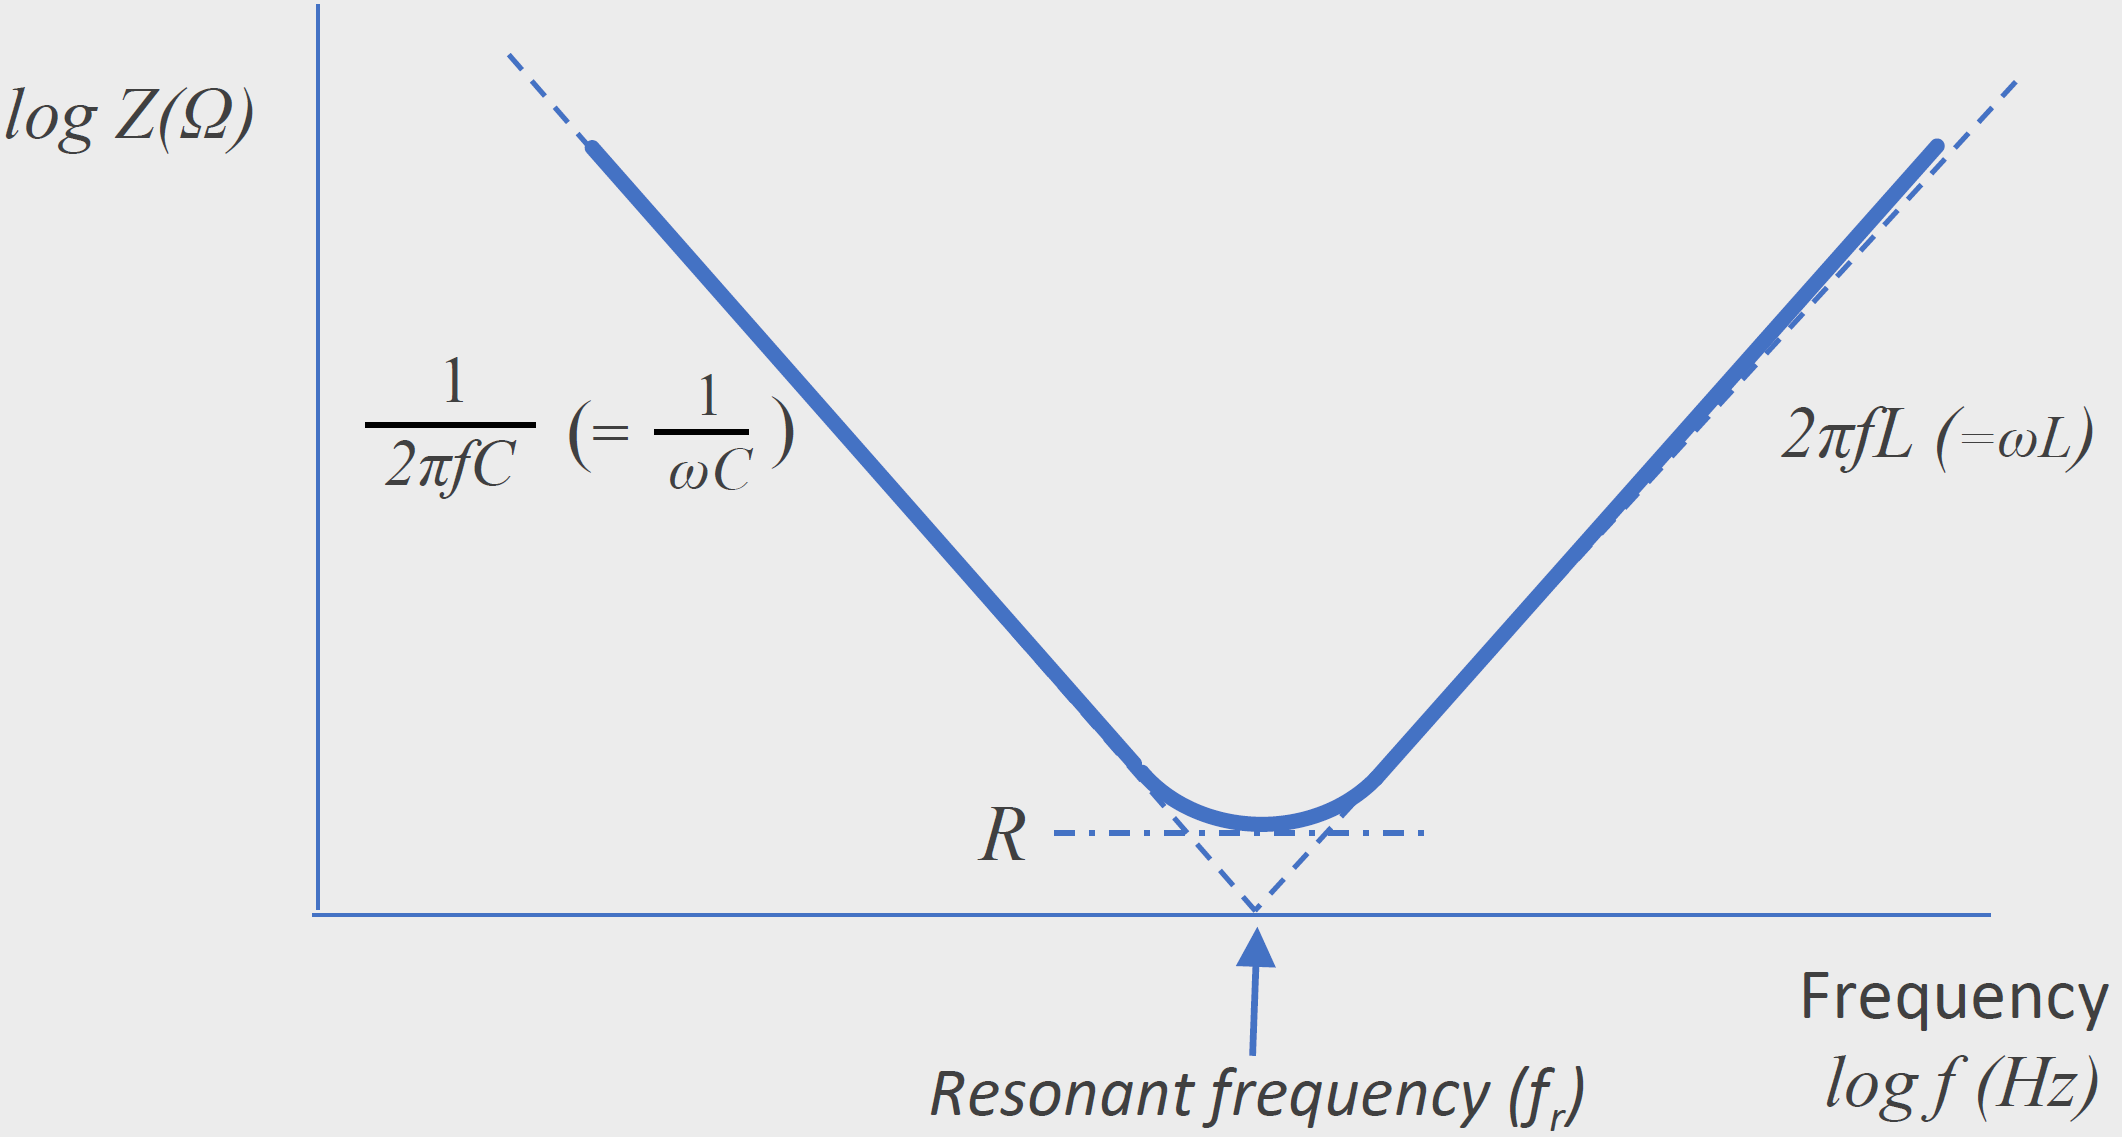
\includegraphics[width=\linewidth]{fig/lec08/impedance_vs_frequency.png}
    \caption{Schematic impedance curve of a real capacitor showing capacitive, resistive, and inductive regions. Adapted from AIC tech, \textit{The Three Essential Characteristics of Capacitors}}
\end{figure}
\end{column}
\end{columns}

\end{frame}


%%%%%%%%%%%%%%%%%%%%%%%%%%%%%%%%%%%%%%%%%%%%%%%%%%%%%%%%%%%%%
%% Self resonant frequency
%%%%%%%%%%%%%%%%%%%%%%%%%%%%%%%%%%%%%%%%%%%%%%%%%%%%%%%%%%%%%
\begin{frame}
\frametitle{Self-Resonant Frequency}
\begin{columns}
\begin{column}{0.56\textwidth}
The self-resonant frequency occurs when the capacitive and inductive reactances cancel:
\begin{align}
    \omega_0 L_{\mathrm{ESL}}
    =
    \frac{1}{\omega_0 C}
\end{align}
\begin{align}
    f_{\mathrm{SRF}}
    =
    \frac{1}{2\pi\sqrt{L_{\mathrm{ESL}}C}}
\end{align}
Below $f_{\mathrm{SRF}}$:
\begin{align}
    |X_C| > |X_L|
\end{align}
and the component behaves mainly as a capacitor. Above $f_{\mathrm{SRF}}$:
\begin{align}
    |X_L| > |X_C|
\end{align}
and the component behaves mainly as an inductor.
\end{column}

\begin{column}{0.40\textwidth}
\begin{block}{Practical Rule}
Do not assume that a large capacitor is useful at all frequencies. Large electrolytics are effective at low frequencies, while small ceramics are effective at much higher frequencies.
\end{block}
\begin{block}{Design Implication}
For high-frequency decoupling, low ESL and short mounting paths are often more important than large capacitance.
\end{block}
\end{column}
\end{columns}
\end{frame}


%%%%%%%%%%%%%%%%%%%%%%%%%%%%%%%%%%%%%%%%%%%%%%%%%%%%%%%%%%%%%
%% Impedance of different capacitor technologies
%%%%%%%%%%%%%%%%%%%%%%%%%%%%%%%%%%%%%%%%%%%%%%%%%%%%%%%%%%%%%
\begin{frame}
\frametitle{Impedance of Different Capacitor Technologies}
\begin{columns}
\begin{column}{0.56\textwidth}
Different capacitor technologies are effective over different frequency ranges.
\begin{itemize}
    \item \textbf{Aluminum electrolytic capacitors}
    \begin{itemize}
        \item high capacitance,
        \item useful for low-frequency energy buffering,
        \item higher ESR and ESL.
    \end{itemize}

    \item \textbf{Film capacitors}
    \begin{itemize}
        \item lower loss,
        \item high ripple-current capability,
        \item useful for DC-link and snubber applications.
    \end{itemize}

    \item \textbf{MLCCs}
    \begin{itemize}
        \item very low ESL,
        \item effective at high frequency,
        \item capacitance may strongly depend on DC bias.
    \end{itemize}
\end{itemize}
A practical converter often uses a capacitor bank combining several technologies.
\end{column}

\begin{column}{0.40\textwidth}
\begin{figure}
    \centering
    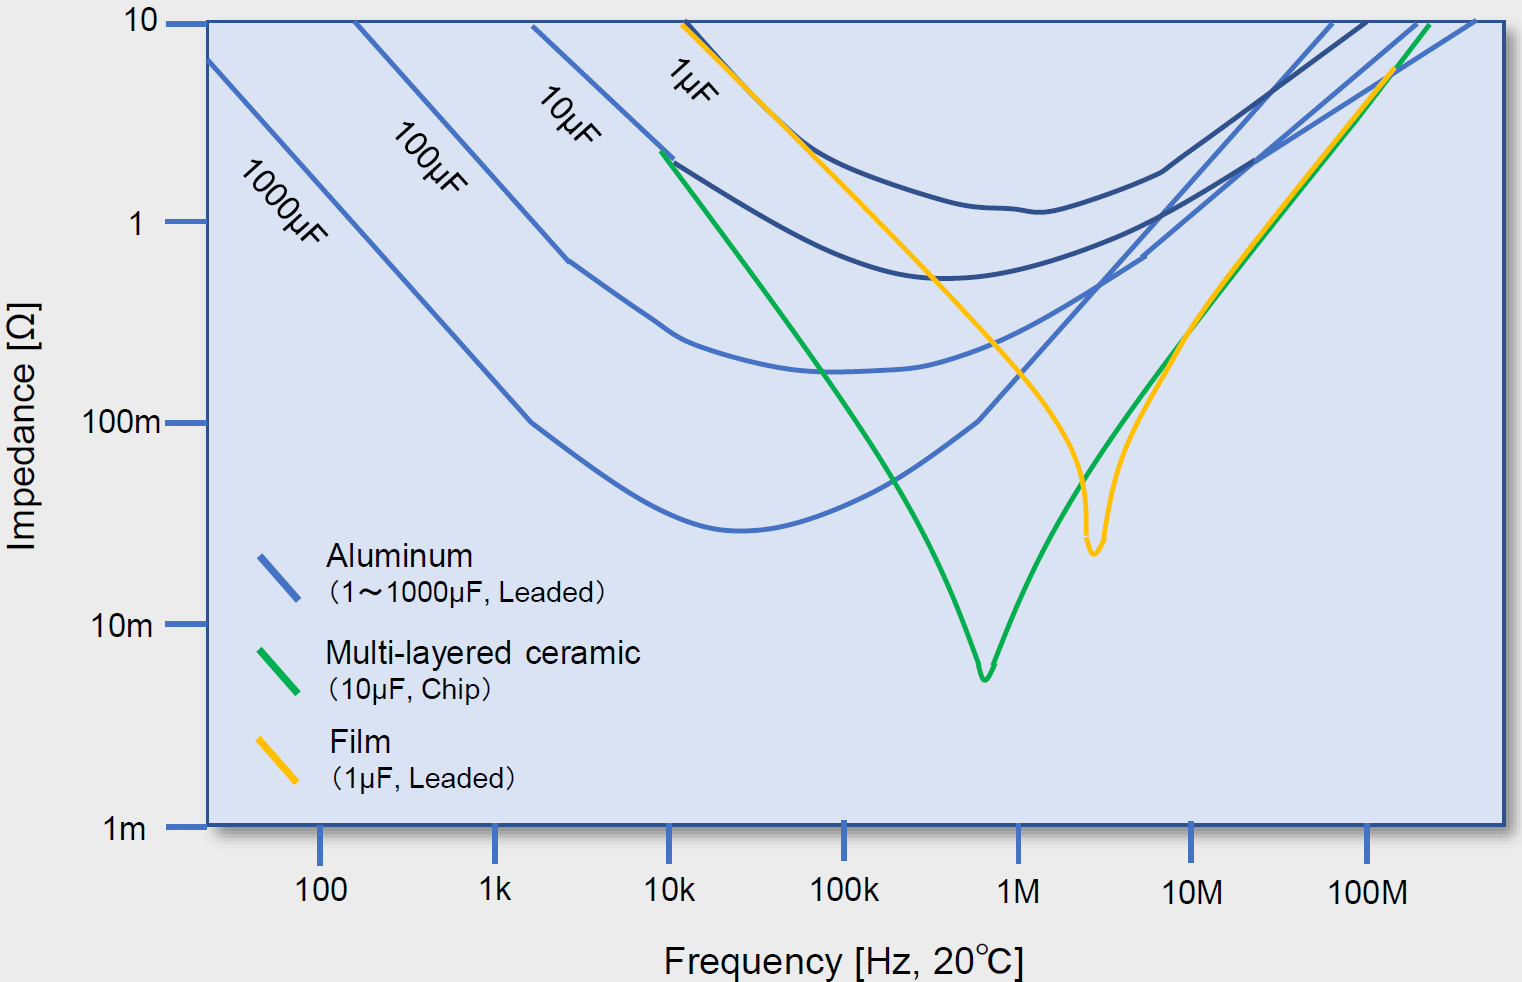
\includegraphics[width=\linewidth]{fig/lec08/impedance_various_capacitors.png}
    \caption{Impedance versus frequency for aluminum electrolytic, film, and multilayer ceramic capacitors. Adapted from AIC tech, \textit{The Three Essential Characteristics of Capacitors}}
\end{figure}
\end{column}
\end{columns}

\end{frame}


%%%%%%%%%%%%%%%%%%%%%%%%%%%%%%%%%%%%%%%%%%%%%%%%%%%%%%%%%%%%%
%% Parallel capacitor networks
%%%%%%%%%%%%%%%%%%%%%%%%%%%%%%%%%%%%%%%%%%%%%%%%%%%%%%%%%%%%%
\begin{frame}
\frametitle{Why are Multiple Capacitors Connected in Parallel?}
\begin{columns}
\begin{column}{0.55\textwidth}
A single capacitor type cannot provide low impedance over a wide frequency range. Therefore, practical converters often combine:
\begin{itemize}
    \item \textbf{bulk capacitor:} low-frequency energy storage,
    \item \textbf{film or polymer capacitor:} mid-frequency ripple current,
    \item \textbf{ceramic capacitor:} high-frequency switching current,
    \item \textbf{local decoupling capacitor:} device-level transient current.
\end{itemize}
For capacitors in parallel,
\begin{align}
    C_{\mathrm{eq}} = C_1+C_2+C_3+\cdots
\end{align}
\end{column}

\begin{column}{0.41\textwidth}
\begin{center}
\begin{circuitikz}[scale=0.78, transform shape]
    \draw (0,0) -- (4.0,0);
    \draw (0,-2.5) -- (4.0,-2.5);

    \draw (0.6,0) to[C,l=$C_{\mathrm{bulk}}$] (0.6,-2.5);
    \draw (1.8,0) to[C,l=$C_{\mathrm{film}}$] (1.8,-2.5);
    \draw (3.0,0) to[C,l=$C_{\mathrm{cer}}$] (3.0,-2.5);

    \draw[->, thick] (-0.5,-1.25) -- (0.2,-1.25);
    \node at (-0.85,-1.25) {$i_C$};

    \node at (0.6,-3.0) {\scriptsize low $f$};
    \node at (1.8,-3.0) {\scriptsize mid $f$};
    \node at (3.0,-3.0) {\scriptsize high $f$};
\end{circuitikz}
\end{center}

\begin{block}{Layout Warning}
The high-frequency capacitor must be physically close to the switching loop. Otherwise PCB and busbar inductance dominate the impedance.
\end{block}
\end{column}
\end{columns}
and ideally ESR and ESL reduce. In practice, layout determines whether this benefit is achieved.
\end{frame}


%%%%%%%%%%%%%%%%%%%%%%%%%%%%%%%%%%%%%%%%%%%%%%%%%%%%%%%%%%%%%
%% Capacitor impedance network
%%%%%%%%%%%%%%%%%%%%%%%%%%%%%%%%%%%%%%%%%%%%%%%%%%%%%%%%%%%%%
\begin{frame}
\frametitle{Impedance Target of a Capacitor Network}
\begin{columns}
\begin{column}{0.56\textwidth}
In a regulator or converter, the objective is usually not to minimize the impedance of one capacitor, but to shape the total impedance of the full capacitor network. Important design ideas:
\begin{itemize}
    \item The bulk capacitor controls low-frequency energy demand.
    \item Polymer or film capacitors reduce mid-frequency impedance.
    \item MLCCs reduce high-frequency impedance.
    \item Excessively low impedance at some frequencies can interact with the control loop and reduce damping.
    \item The impedance at the actual load terminals can differ from the impedance at the regulator terminals due to PCB parasitics.
\end{itemize}
Therefore, capacitor selection should be performed together with layout and stability analysis.
\end{column}

\begin{column}{0.40\textwidth}
\begin{figure}
    \centering
    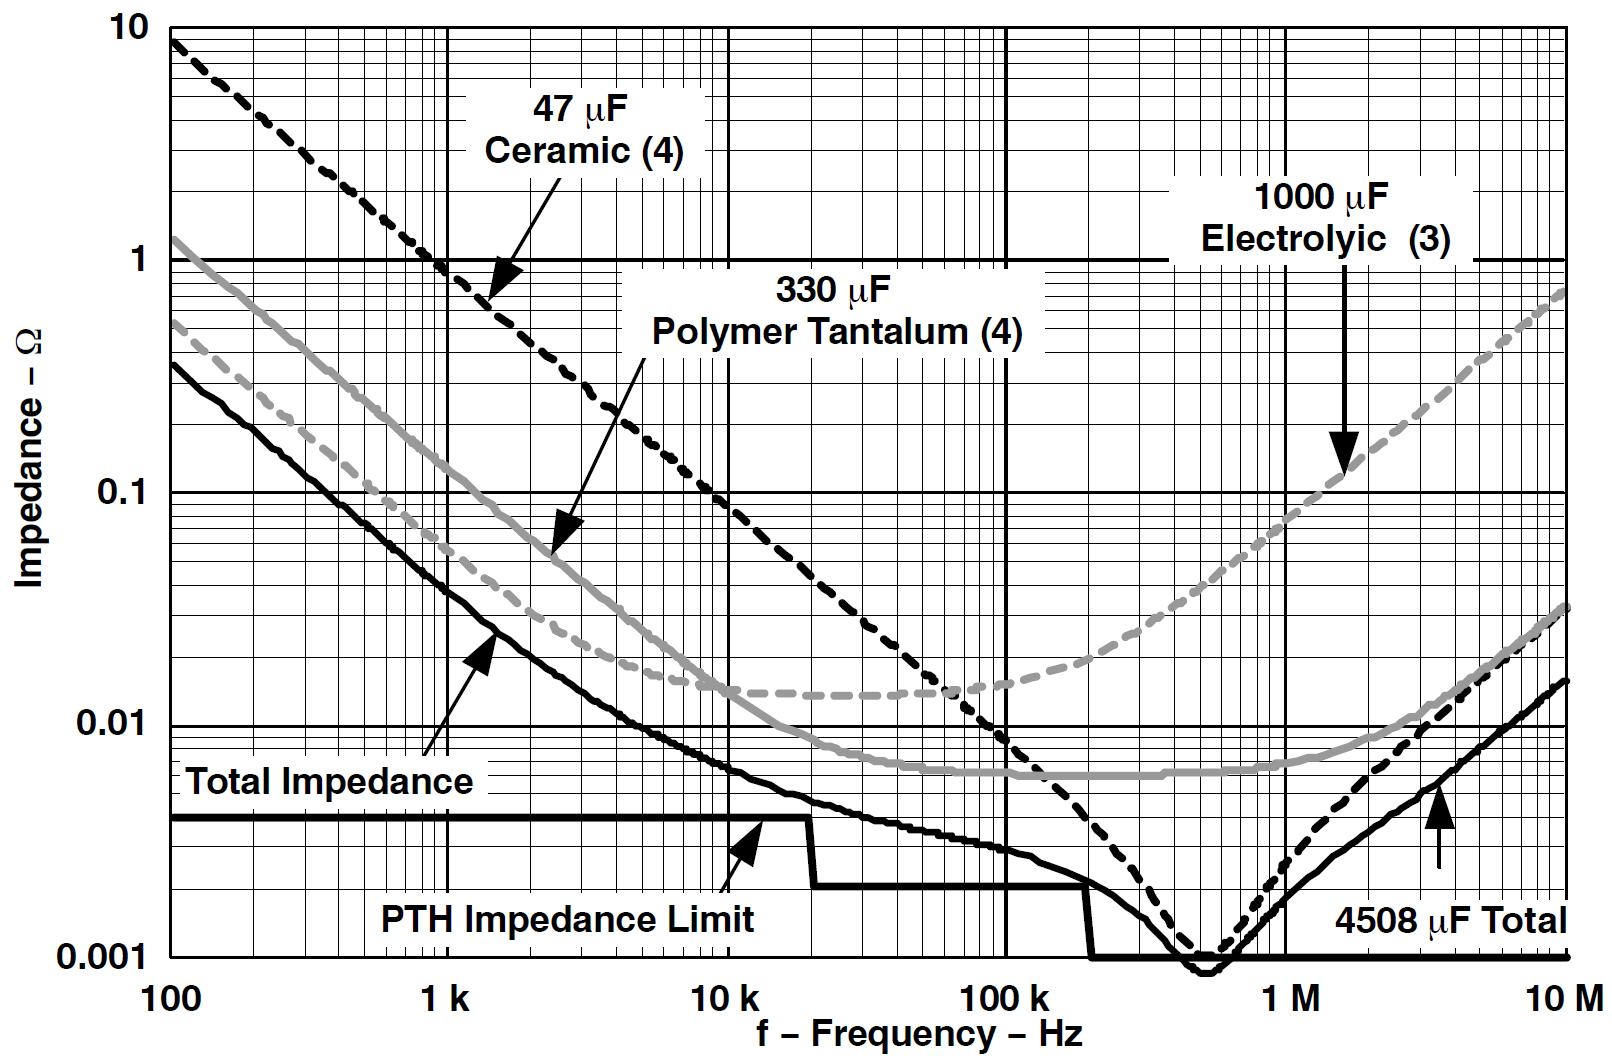
\includegraphics[width=\linewidth]{fig/lec08/impedance_limits.png}
    \caption{Output capacitor impedance limits and combined impedance of electrolytic, polymer tantalum, and ceramic capacitor networks. Adapted from Texas Instruments, \textit{Input and Output Capacitor Selection}}
\end{figure}
\end{column}
\end{columns}
\end{frame}


%%%%%%%%%%%%%%%%%%%%%%%%%%%%%%%%%%%%%%%%%%%%%%%%%%%%%%%%%%%%%
%% Leakage current
%%%%%%%%%%%%%%%%%%%%%%%%%%%%%%%%%%%%%%%%%%%%%%%%%%%%%%%%%%%%%
\begin{frame}
\frametitle{Leakage Current and Insulation Resistance}

\begin{columns}
\begin{column}{0.5\textwidth}
A real capacitor does not perfectly block DC. A small leakage current flows through or around the dielectric. Leakage current can be represented by an insulation resistance in parallel with the capacitance:
\begin{align}
    i_{\mathrm{leak}}
    =
    \frac{V}{R_{\mathrm{iso}}}
\end{align}
where,
\begin{itemize}
    \item $i_{\mathrm{leak}}$ is leakage current,
    \item $V$ is applied voltage,
    \item $R_{\mathrm{iso}}$ is insulation resistance.
\end{itemize}

\end{column}

\begin{column}{0.5\textwidth}
    Leakage current is important for:
\begin{itemize}
    \item DC-link discharge behaviour,
    \item capacitor bank voltage balancing,
    \item standby power loss,
    \item safety after shutdown,
    \item health monitoring and ageing assessment.
\end{itemize}
\begin{figure}
    \centering
    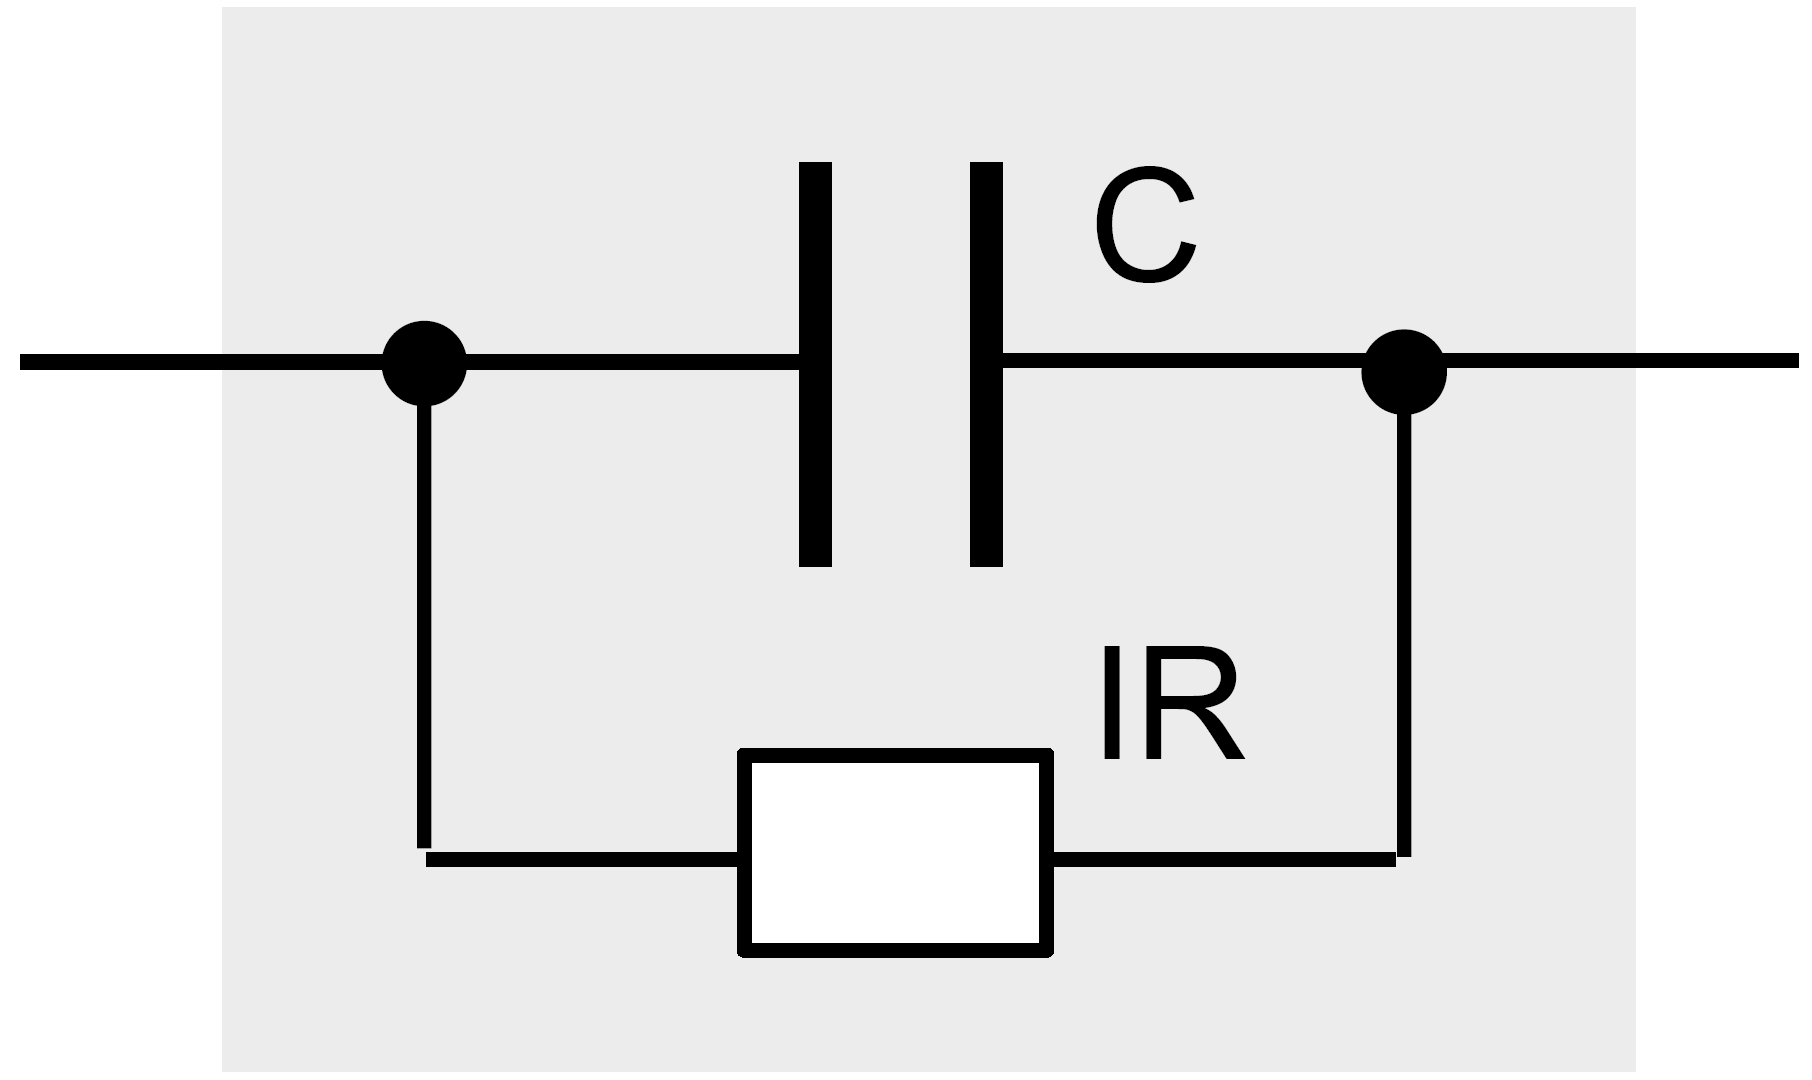
\includegraphics[width=0.3\linewidth]{fig/lec08/capacitance_insulation_resistance.png}
    \caption{Leakage current represented by insulation resistance in parallel with capacitance. Adapted from AIC tech, \textit{The Three Essential Characteristics of Capacitors}}
\end{figure}
\end{column}
\end{columns}

\end{frame}


%%%%%%%%%%%%%%%%%%%%%%%%%%%%%%%%%%%%%%%%%%%%%%%%%%%%%%%%%%%%%
%% Leakage current dependence
%%%%%%%%%%%%%%%%%%%%%%%%%%%%%%%%%%%%%%%%%%%%%%%%%%%%%%%%%%%%%
\begin{frame}
\frametitle{Leakage Current Depends on Voltage, Temperature, and History}
\begin{columns}
\begin{column}{0.56\textwidth}
Leakage current is not a fixed constant. It depends strongly on operating condition and capacitor technology. Important dependencies:
\begin{itemize}
    \item Leakage current increases with applied voltage.
    \item Leakage current usually increases with temperature.
    \item Electrolytic capacitor leakage depends on formation condition and voltage history.
    \item Humidity, contamination, dielectric defects, and ageing can increase leakage.
\end{itemize}
For capacitor banks, leakage mismatch is especially important because it can cause unequal voltage sharing between series-connected capacitors. Therefore, series capacitor banks usually require voltage-balancing resistors.
\end{column}

\begin{column}{0.40\textwidth}
\begin{figure}
    \centering
    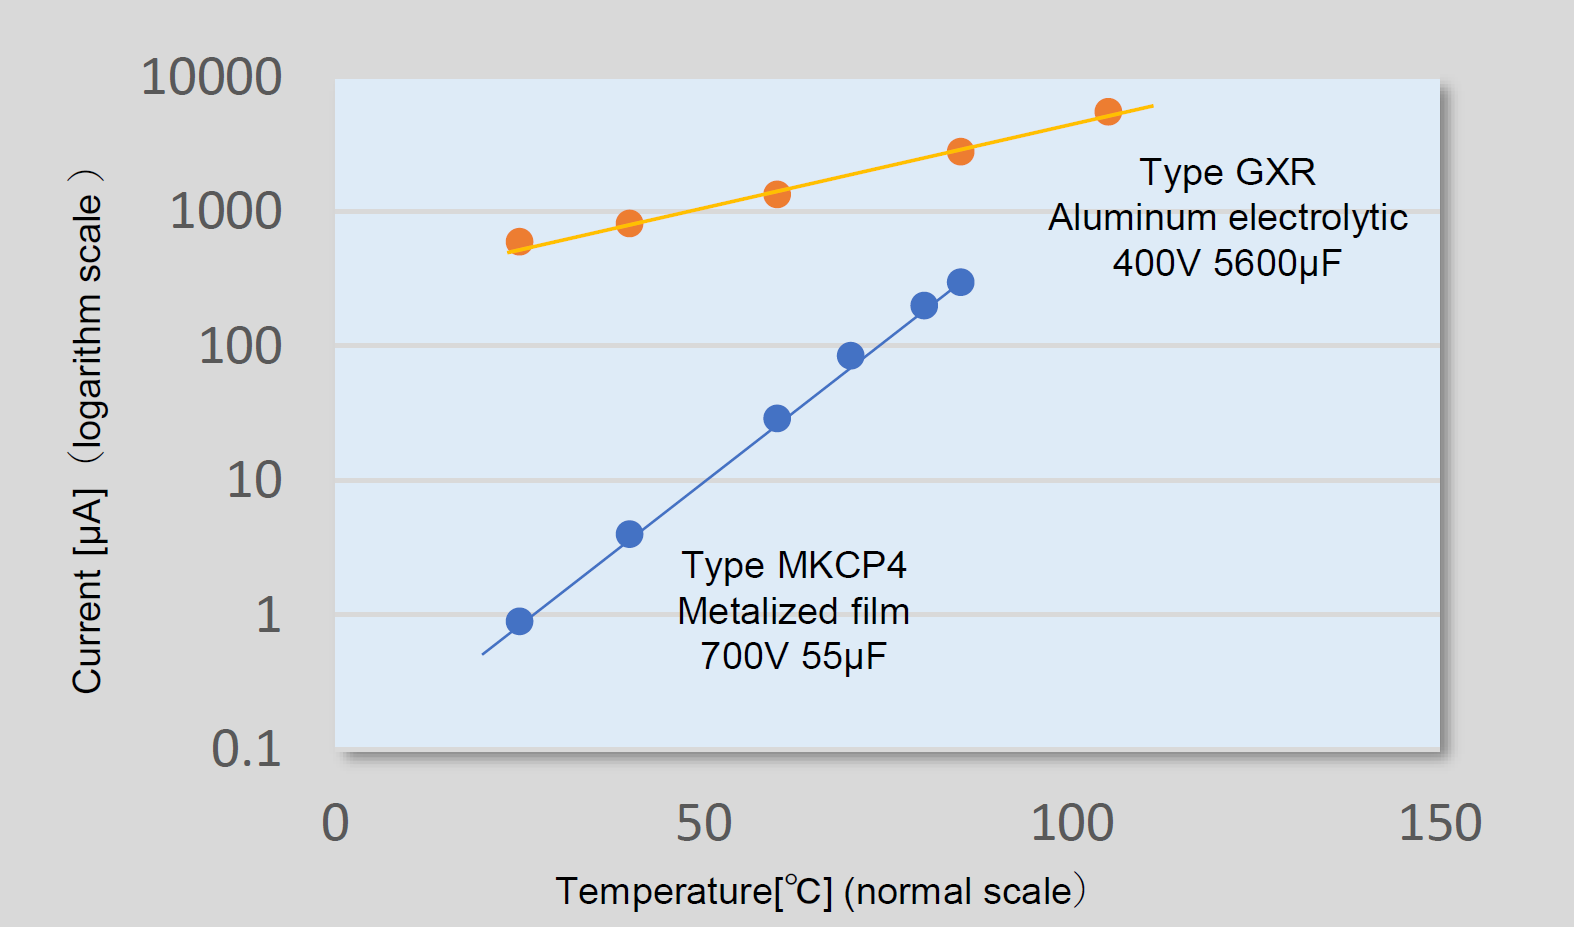
\includegraphics[width=\linewidth]{fig/lec08/leakage_temperature.png}
    \caption{Leakage current versus temperature for aluminum electrolytic and metallized film capacitors. Adapted from AIC tech, \textit{The Three Essential Characteristics of Capacitors}}
\end{figure}
\end{column}
\end{columns}

\end{frame}


%%%%%%%%%%%%%%%%%%%%%%%%%%%%%%%%%%%%%%%%%%%%%%%%%%%%%%%%%%%%%
%% Dissipation factor and tan delta
%%%%%%%%%%%%%%%%%%%%%%%%%%%%%%%%%%%%%%%%%%%%%%%%%%%%%%%%%%%%%
\begin{frame}
\frametitle{Dissipation Factor and $\tan\delta$}
\begin{columns}
\begin{column}{0.56\textwidth}
In an ideal capacitor, the current leads the voltage by exactly $90^\circ$. In a real capacitor, losses reduce this phase angle slightly. The dissipation factor is commonly written as
\begin{align}
    \tan\delta
    =
    \frac{R_{\mathrm{ESR}}}{X_C}
    =
    \omega C R_{\mathrm{ESR}}
\end{align}
where
\begin{align}
    X_C=\frac{1}{\omega C}
\end{align}
A smaller $\tan\delta$ means lower dielectric and resistive loss. For sinusoidal operation, dielectric loss can be estimated using
\begin{align}
    P_{\mathrm{diel}}
    =
    \omega C V_{\mathrm{rms}}^2 \tan\delta
\end{align}
\end{column}

\begin{column}{0.40\textwidth}
\begin{figure}
    \centering
    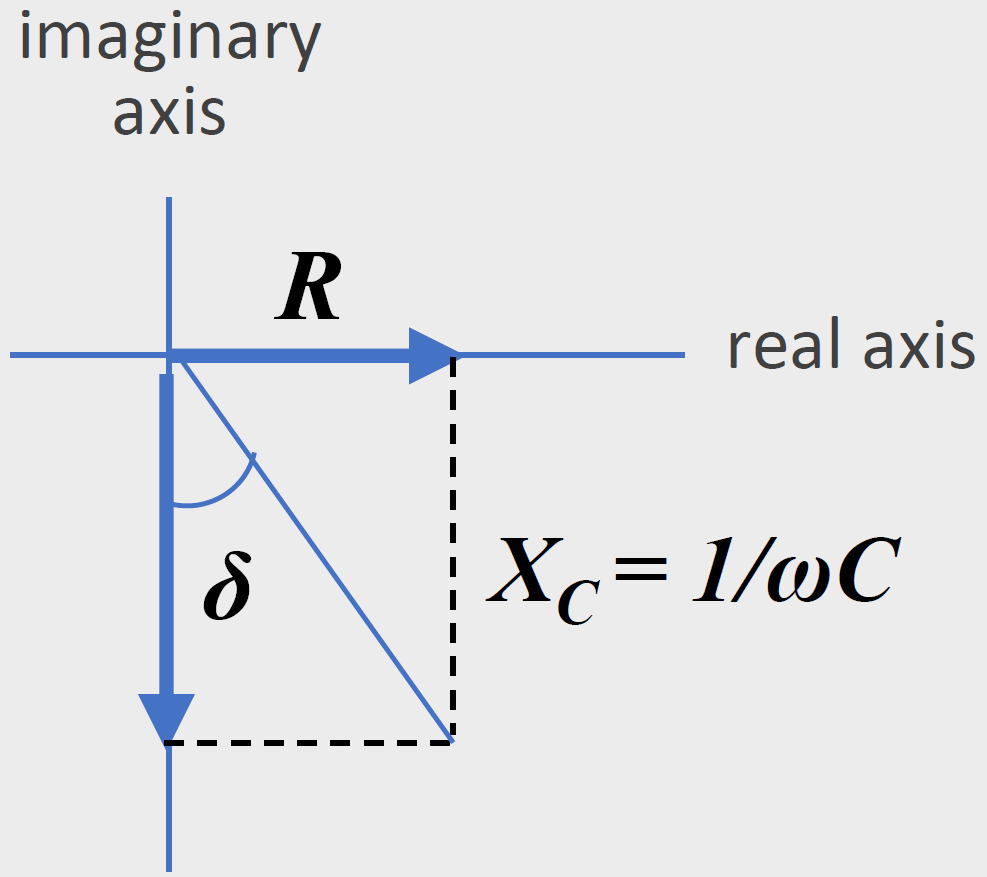
\includegraphics[width=0.5\linewidth]{fig/lec08/vector_R_Xc_tandelta.png}
    \caption{Vector expression of resistance and capacitive reactance used to define $\tan\delta$. Adapted from AIC tech, \textit{The Three Essential Characteristics of Capacitors}}
\end{figure}
\end{column}
\end{columns}

\end{frame}


%%%%%%%%%%%%%%%%%%%%%%%%%%%%%%%%%%%%%%%%%%%%%%%%%%%%%%%%%%%%%
%% Equivalent circuit for sinusoidal loss
%%%%%%%%%%%%%%%%%%%%%%%%%%%%%%%%%%%%%%%%%%%%%%%%%%%%%%%%%%%%%
\begin{frame}
\frametitle{Equivalent Circuits for Capacitor Losses}
\begin{columns}
\begin{column}{0.56\textwidth}
Capacitor losses are often represented using either a parallel or series equivalent circuit. For sinusoidal operation, the two forms can be transformed into one another. The series representation is especially useful in power electronics because ripple current directly produces ESR loss:
\begin{align}
    P_{\mathrm{loss}}
    =
    I_{\mathrm{rms}}^2R_{\mathrm{ESR}}
\end{align}
The parallel representation is useful for interpreting insulation resistance and dielectric leakage. For non-sinusoidal power-converter waveforms, losses should be evaluated from the harmonic content or measured under realistic operating conditions.
\end{column}

\begin{column}{0.40\textwidth}
\begin{figure}
    \centering
    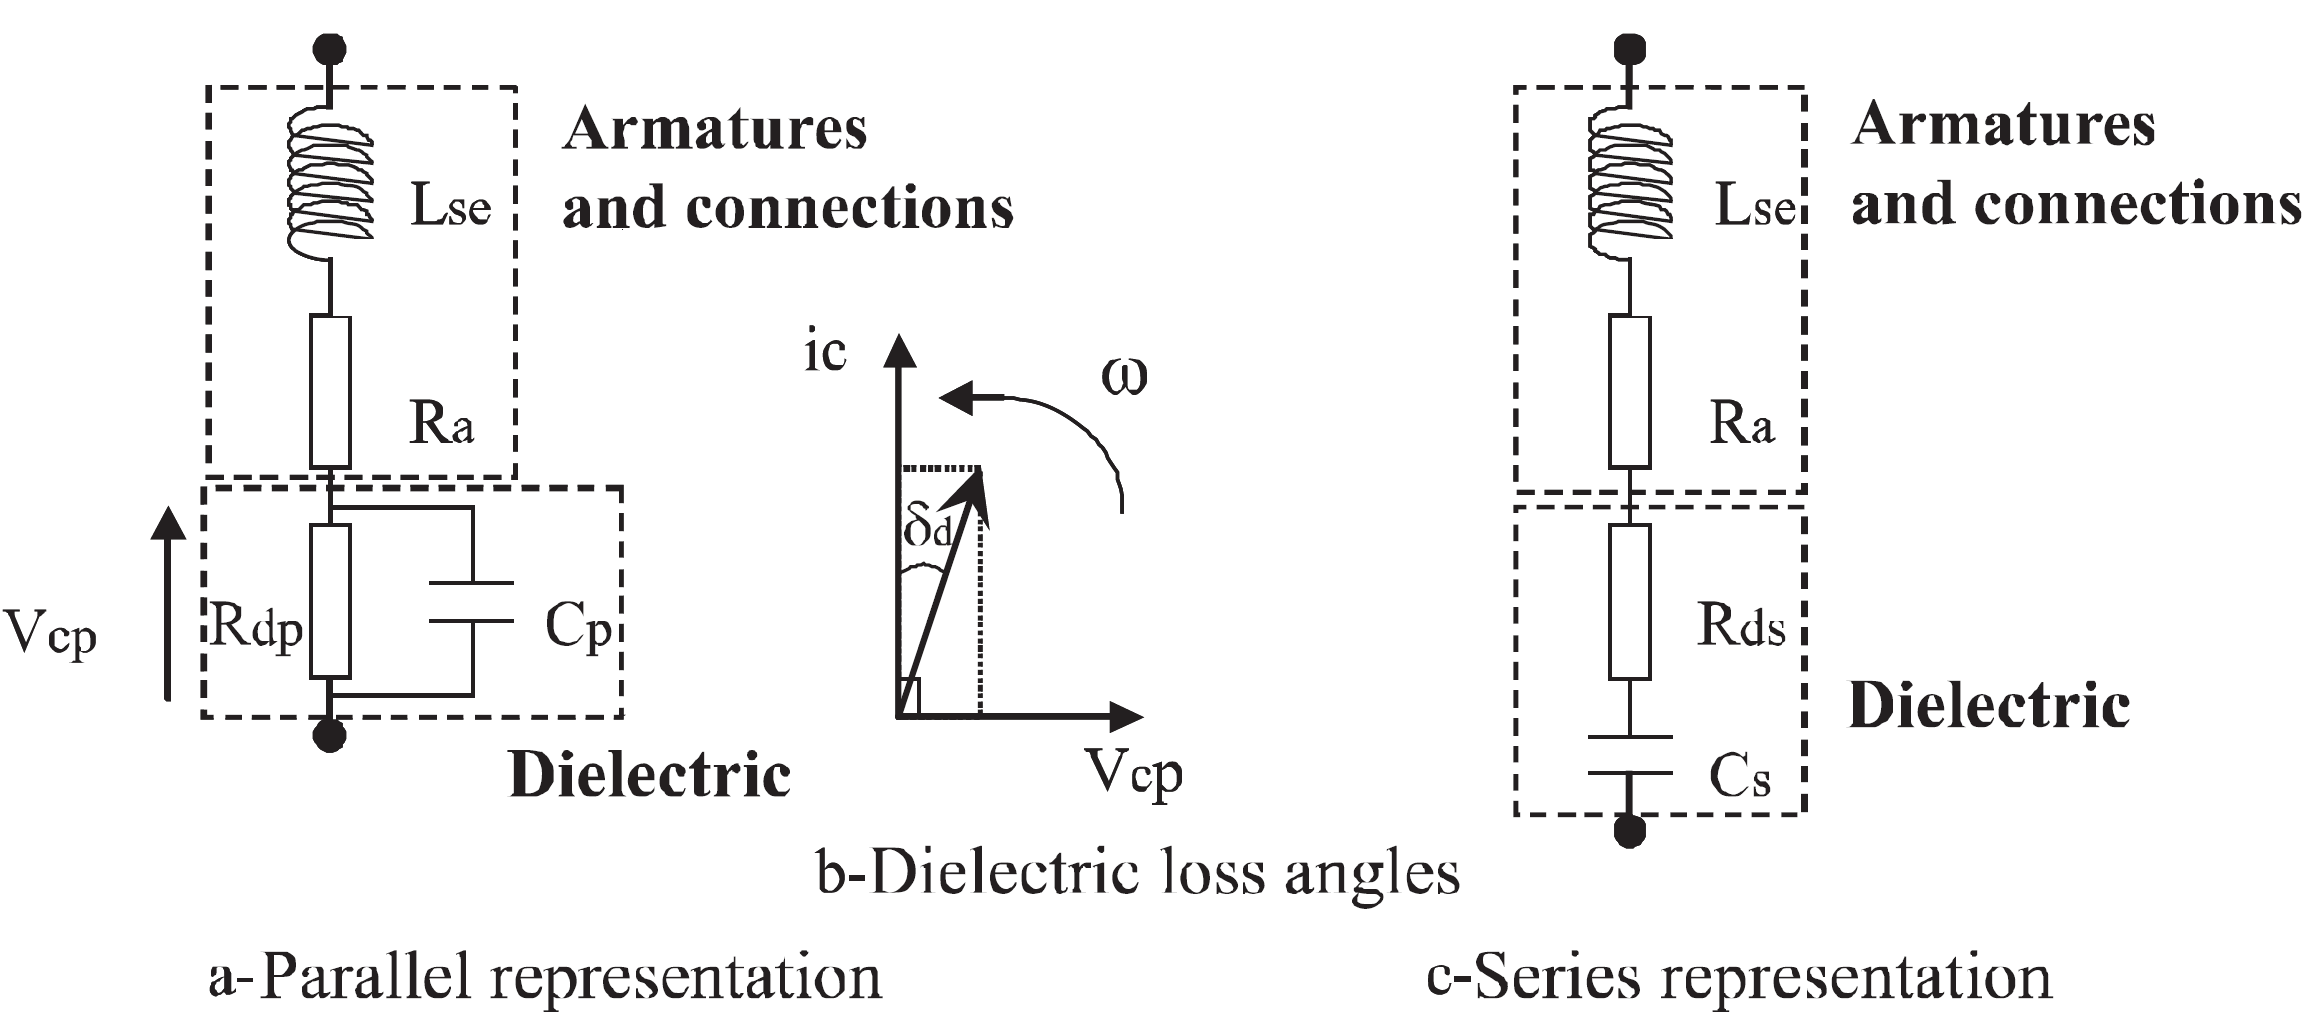
\includegraphics[width=\linewidth]{fig/lec08/capacitor_equivalent_circuits.png}
    \caption{Parallel and series equivalent electrical circuits of a capacitor under sinusoidal operation. Adapted from Perret, \textit{Power Electronics Semiconductor Devices}, Wiley, 2009.}
\end{figure}
\end{column}
\end{columns}
\end{frame}


%%%%%%%%%%%%%%%%%%%%%%%%%%%%%%%%%%%%%%%%%%%%%%%%%%%%%%%%%%%%%
%% Dielectric absorption
%%%%%%%%%%%%%%%%%%%%%%%%%%%%%%%%%%%%%%%%%%%%%%%%%%%%%%%%%%%%%
\begin{frame}
\frametitle{Dielectric Absorption and Recovery Voltage}

\begin{columns}
\begin{column}{0.56\textwidth}
Dielectric absorption is when a capacitor regains a small voltage after being discharged and left open-circuited:
\begin{itemize}
    \item Polarization processes inside the dielectric are not instantaneous.
    \item Some dipoles relax slowly after the external voltage is removed.
    \item Charge redistribution can produce a residual recovery voltage.
\end{itemize}
\end{column}

\begin{column}{0.40\textwidth}
\begin{figure}
    \centering
    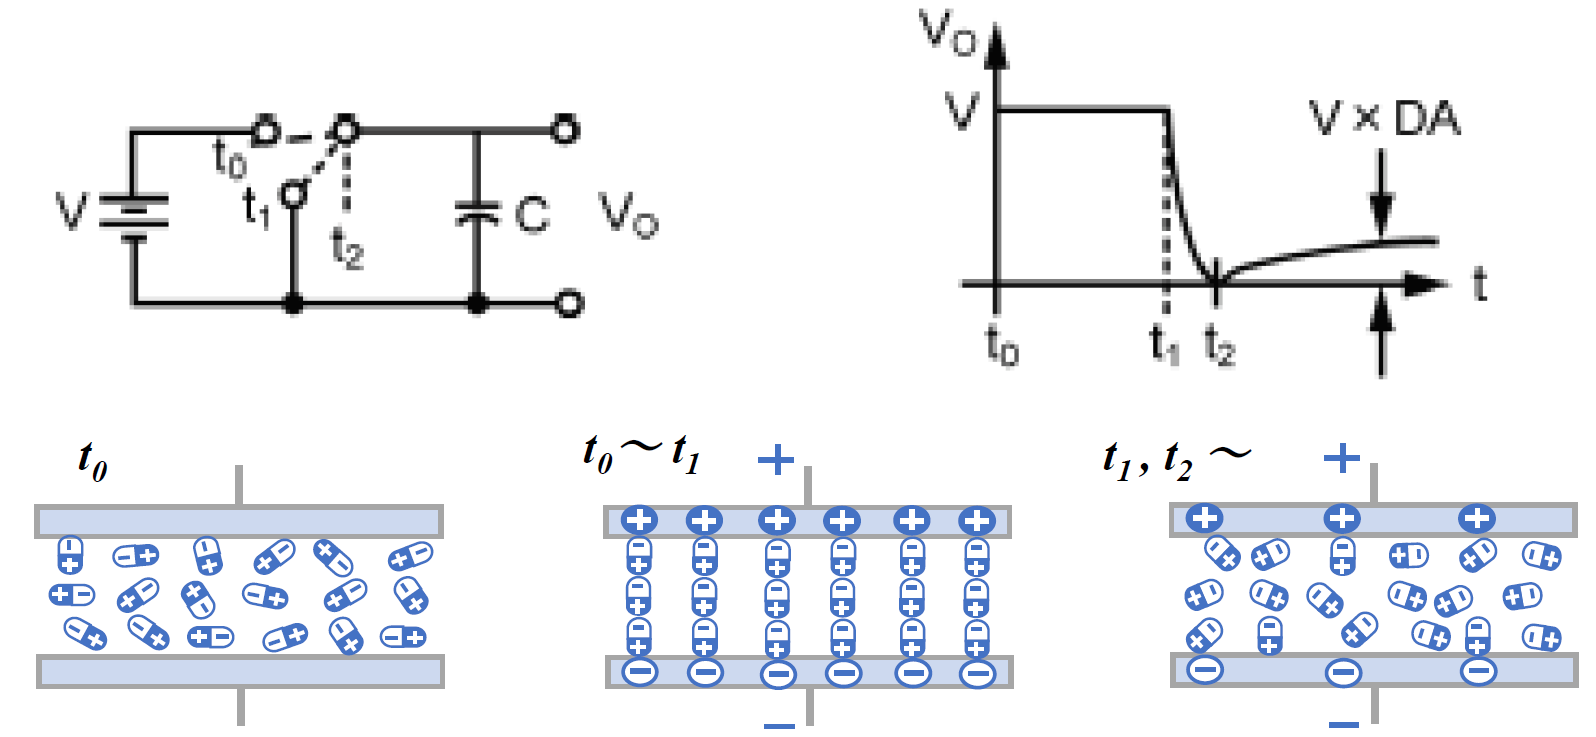
\includegraphics[width=\linewidth]{fig/lec08/dielectric_absorption_and_recovery_voltage.png}
    \caption{Dielectric absorption and recovery voltage after short-circuit discharge. Adapted from AIC tech, \textit{The Three Essential Characteristics of Capacitors}}
\end{figure}
\end{column}
\end{columns}

\end{frame}



%%%%%%%%%%%%%%%%%%%%%%%%%%%%%%%%%%%%%%%%%%%%%%%%%%%%%%%%%%%%%
%% Dielectric absorption
%%%%%%%%%%%%%%%%%%%%%%%%%%%%%%%%%%%%%%%%%%%%%%%%%%%%%%%%%%%%%
\begin{frame}
\frametitle{Dielectric Absorption and Recovery Voltage}
\begin{columns}
\begin{column}{0.56\textwidth}
Dielectric absorption effect is important in:
\begin{itemize}
    \item precision sampling circuits,
    \item high-voltage DC-link safety,
    \item insulation testing,
    \item pulse capacitors,
    \item stored-energy applications.
\end{itemize}
A discharged capacitor should therefore still be treated carefully in high-voltage systems.
\end{column}

\begin{column}{0.40\textwidth}
\begin{block}{Practical Safety Message}
\small
Large capacitors may show recovery voltage after discharge due to dielectric absorption. Discharge resistors and voltage verification are required before handling high-energy capacitor banks.
\end{block}
\end{column}
\end{columns}
\end{frame}


%%%%%%%%%%%%%%%%%%%%%%%%%%%%%%%%%%%%%%%%%%%%%%%%%%%%%%%%%%%%%
%% Real capacitor design summary
%%%%%%%%%%%%%%%%%%%%%%%%%%%%%%%%%%%%%%%%%%%%%%%%%%%%%%%%%%%%%
\begin{frame}
\frametitle{Summary: What Defines a Real Capacitor?}
\begin{itemize}
    \item Capacitance determines ideal charge storage: $Q=CV$.
    \item ESR determines ripple-current heating: $P_{\mathrm{ESR}}=I_{\mathrm{rms}}^2R_{\mathrm{ESR}}$.
    \item ESL determines high-frequency voltage spikes:
    \begin{align}
        v_{\mathrm{ESL}}=L_{\mathrm{ESL}}\frac{di}{dt}
    \end{align}
    \item Self-resonant frequency separates capacitive and inductive behaviour:
    \begin{align}
        f_{\mathrm{SRF}}=\frac{1}{2\pi\sqrt{L_{\mathrm{ESL}}C}}
    \end{align}
    \item Leakage current affects safety, voltage balancing, standby loss, and ageing:
    \begin{align}
        i_{\mathrm{leak}}=\frac{V}{R_{\mathrm{iso}}}
    \end{align}
    \item In power electronics, the useful capacitor is the one that gives the required impedance, ripple-current capability, thermal margin, and lifetime in the actual converter layout.
\end{itemize}

\end{frame}

%%%%%%%%%%%%%%%%%%%%%%%%%%%%%%%%%%%%%%%%%%%%%%%%%%%%%%%%%%%%%
%% Capacitors in converter applications
%%%%%%%%%%%%%%%%%%%%%%%%%%%%%%%%%%%%%%%%%%%%%%%%%%%%%%%%%%%%%
\begin{frame}
\begin{center}
  \textbf{\Huge{Capacitors in Converter Applications}}\\[0.4cm]
  \textbf{\Large{Input, Output, DC-Link, Snubber, Resonant, and Filter Capacitors}}
\end{center}
\end{frame}


%%%%%%%%%%%%%%%%%%%%%%%%%%%%%%%%%%%%%%%%%%%%%%%%%%%%%%%%%%%%%
%% Capacitor placement in power converters
%%%%%%%%%%%%%%%%%%%%%%%%%%%%%%%%%%%%%%%%%%%%%%%%%%%%%%%%%%%%%
\begin{frame}
\frametitle{Where are Capacitors Used in a Power Converter?}

\begin{columns}
\begin{column}{0.58\textwidth}
Capacitors appear at several locations in a power electronic system. Each location imposes different stress and requires a distinct design approach.
\begin{itemize}
    \item \textbf{Input filter capacitor:} reduces source-side ripple and reflected switching noise.
    \item \textbf{DC-link capacitor:} buffers energy and stabilizes the intermediate DC voltage.
    \item \textbf{Local decoupling capacitor:} supplies very fast switching current close to semiconductor devices.
    \item \textbf{Snubber capacitor:} limits overvoltage during switching transients.
    \item \textbf{Output capacitor:} reduces output-voltage ripple and supports load transients.
    \item \textbf{AC harmonic filter capacitor:} attenuates switching-frequency harmonics at the AC side.
\end{itemize}
Thus, capacitor selection must always begin with the converter function.
\end{column}

\begin{column}{0.38\textwidth}
\begin{figure}
    \centering
    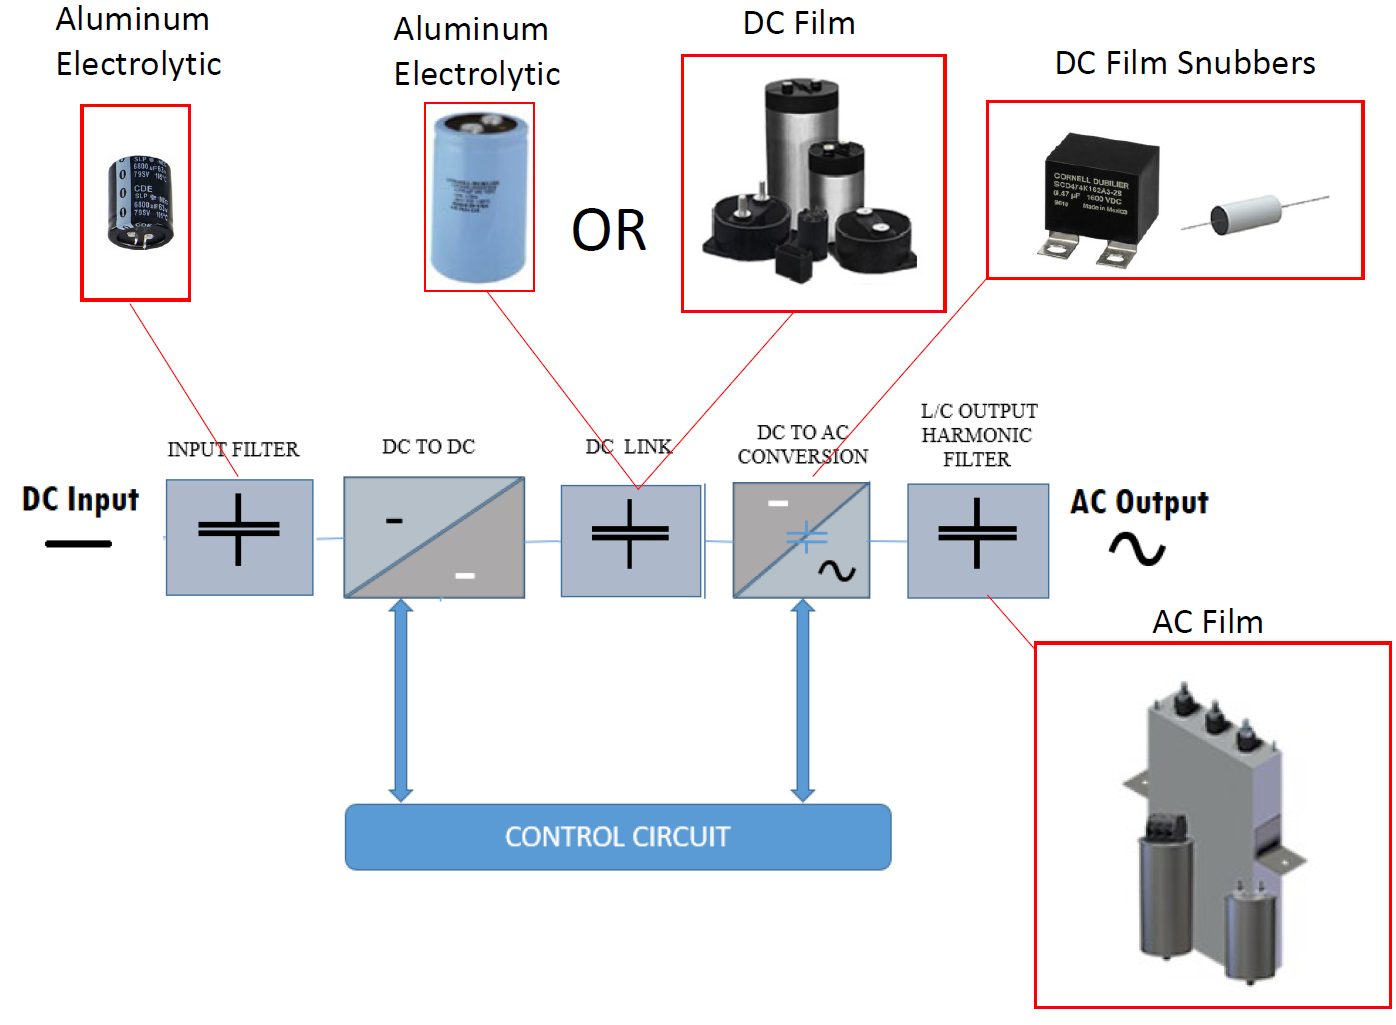
\includegraphics[width=\linewidth]{fig/lec08/capacitors_types.png}
    \caption{Capacitor locations in inverter and converter systems: input filter, DC-link, snubber, and AC harmonic filter. Adapted from Cornell Dubilier, \textit{Capacitors for High Power Inverters and Converters}}
\end{figure}
\end{column}
\end{columns}

\end{frame}


%%%%%%%%%%%%%%%%%%%%%%%%%%%%%%%%%%%%%%%%%%%%%%%%%%%%%%%%%%%%%
%% Application map using circuitikz
%%%%%%%%%%%%%%%%%%%%%%%%%%%%%%%%%%%%%%%%%%%%%%%%%%%%%%%%%%%%%
\begin{frame}
\frametitle{Capacitor Function Map in a Converter}
\begin{center}
\begin{circuitikz}[scale=0.77, transform shape]
    \tikzstyle{block} = [draw, rounded corners, align=center,
    minimum width=2.35cm, minimum height=0.78cm, font=\scriptsize]

    \node[block] (source) at (0,0) {DC or AC\\source};
    \node[block] (input) at (2.8,0) {Input\\filter};
    \node[block] (stage1) at (5.6,0) {Rectifier /\\DC--DC};
    \node[block] (dclink) at (8.4,0) {DC link};
    \node[block] (stage2) at (11.2,0) {Inverter /\\DC--DC};
    \node[block] (output) at (14.0,0) {Output\\filter};
    \node[block] (load) at (16.6,0) {Load};

    \draw[->, thick] (source) -- (input);
    \draw[->, thick] (input) -- (stage1);
    \draw[->, thick] (stage1) -- (dclink);
    \draw[->, thick] (dclink) -- (stage2);
    \draw[->, thick] (stage2) -- (output);
    \draw[->, thick] (output) -- (load);

    \node at (2.8,-1.05) {\scriptsize $C_{\mathrm{in}}$};
    \node at (8.4,-1.05) {\scriptsize $C_{\mathrm{dc}}$};
    \node at (11.2,-1.05) {\scriptsize $C_{\mathrm{snub}}$};
    \node at (14.0,-1.05) {\scriptsize $C_{\mathrm{out}}$};

    \draw (2.8,-0.55) to[C] (2.8,-1.55);
    \draw (8.4,-0.55) to[C] (8.4,-1.55);
    \draw (11.2,-0.55) to[C] (11.2,-1.55);
    \draw (14.0,-0.55) to[C] (14.0,-1.55);

    \node[align=center, font=\scriptsize] at (2.8,-2.05) {ripple and\\EMI reduction};
    \node[align=center, font=\scriptsize] at (8.4,-2.05) {energy buffer and\\DC-bus stabilization};
    \node[align=center, font=\scriptsize] at (11.2,-2.05) {switching\\overvoltage control};
    \node[align=center, font=\scriptsize] at (14.0,-2.05) {output ripple and\\transient support};
\end{circuitikz}
\end{center}

\begin{block}{Teaching Message}
The same symbol \(C\) can represent very different hardware requirements depending on its converter location. A DC-link capacitor, snubber capacitor, and output capacitor are not interchangeable design objects.
\end{block}

\end{frame}


%%%%%%%%%%%%%%%%%%%%%%%%%%%%%%%%%%%%%%%%%%%%%%%%%%%%%%%%%%%%%
%% Input capacitor in buck converter
%%%%%%%%%%%%%%%%%%%%%%%%%%%%%%%%%%%%%%%%%%%%%%%%%%%%%%%%%%%%%
\begin{frame}
\frametitle{Input Capacitor in a Buck Converter}

\begin{columns}
\begin{column}{0.56\textwidth}
The buck input capacitor supplies the switch-node pulsed current and limits input-source ripple voltage. For a single-phase buck converter:
\begin{itemize}
    \item the input capacitor current is strongly pulsed,
    \item the RMS ripple current depends on duty cycle,
    \item worst ripple-current stress near \(D=0.5\),
    \item ceramic capacitors are required close to the switching stage for high-frequency ripple control,
    \item bulk capacitors alone are usually not sufficient because of ESR and ESL.
\end{itemize}
\end{column}

\begin{column}{0.40\textwidth}
\begin{figure}
    \centering
    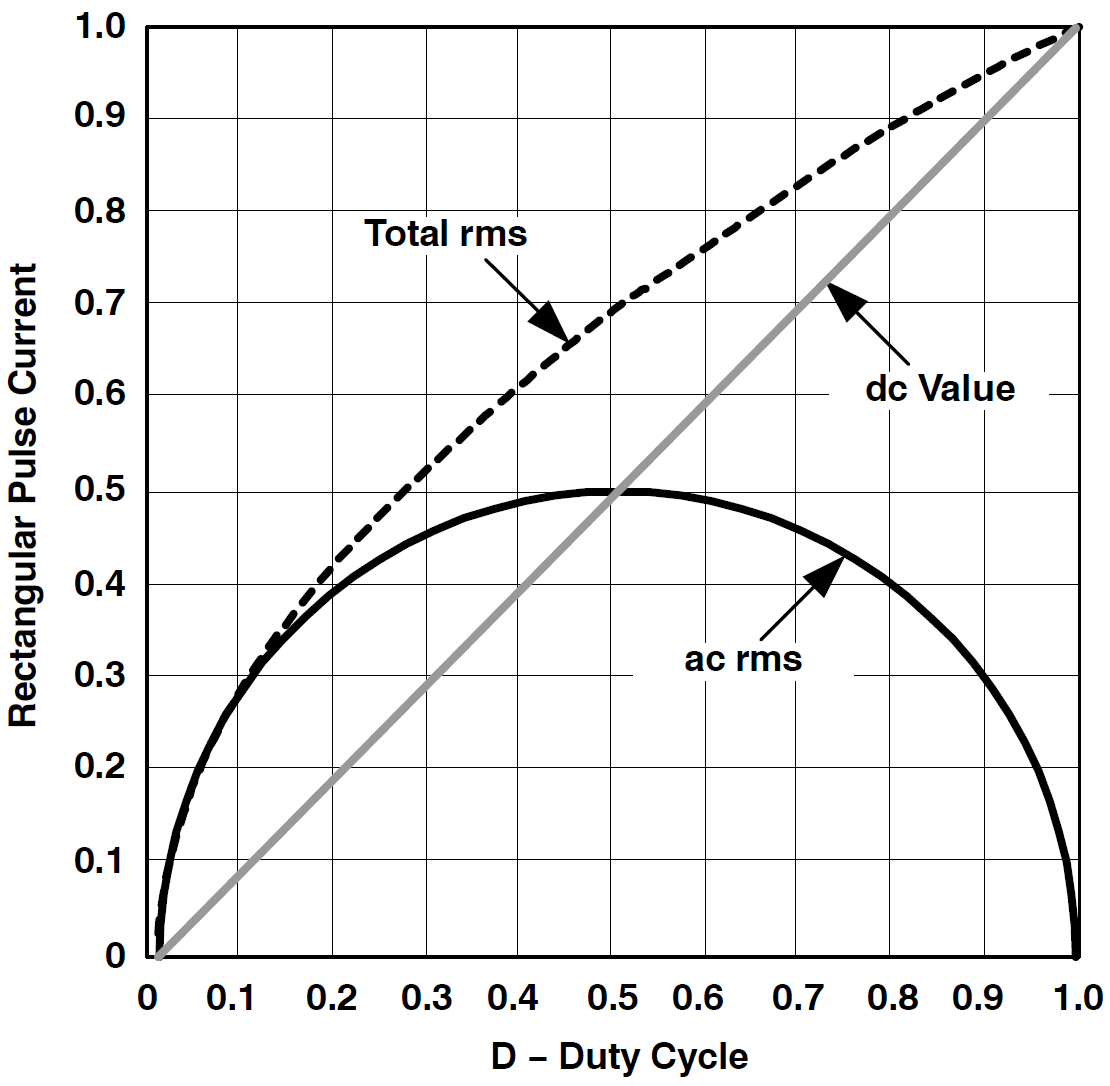
\includegraphics[width=0.8\linewidth]{fig/lec08/input_pulse_current_duty_cycle.png}
    \caption{Input pulse-current components versus duty cycle for a single-phase buck regulator. Adapted from Texas Instruments, \textit{Input and Output Capacitor Selection}, SLTA055}
\end{figure}
\end{column}
\end{columns}

\end{frame}


%%%%%%%%%%%%%%%%%%%%%%%%%%%%%%%%%%%%%%%%%%%%%%%%%%%%%%%%%%%%%
%% Input ceramic capacitance
%%%%%%%%%%%%%%%%%%%%%%%%%%%%%%%%%%%%%%%%%%%%%%%%%%%%%%%%%%%%%
\begin{frame}
\frametitle{Input Ceramic Capacitor Sizing}

\begin{columns}
\begin{column}{0.56\textwidth}
A first estimate of the required input ceramic capacitance for a buck regulator can be obtained from the allowable input ripple voltage. For a triangular charge-balance approximation,
\begin{align}
    C_{\mathrm{in,min}}
    \approx
    \frac{I_oD(1-D)}
    {f_s\Delta V_{\mathrm{in,pp}}}
\end{align}
where
\begin{itemize}
    \item \(I_o\) is the output load current,
    \item \(D\) is duty cycle,
    \item \(f_s\) is switching frequency,
    \item \(\Delta V_{\mathrm{in,pp}}\) is allowable peak-to-peak input ripple.
\end{itemize}
\end{column}

\begin{column}{0.40\textwidth}
\begin{block}{Important Practical Note}
\small
Texas Instruments recommends using the effective ceramic capacitance at operating DC voltage, not only the nominal datasheet value. In MLCCs, the effective capacitance can be much smaller than the rated value.
\end{block}
\end{column}
\end{columns}

\end{frame}


%%%%%%%%%%%%%%%%%%%%%%%%%%%%%%%%%%%%%%%%%%%%%%%%%%%%%%%%%%%%%
%% Input ceramic capacitance
%%%%%%%%%%%%%%%%%%%%%%%%%%%%%%%%%%%%%%%%%%%%%%%%%%%%%%%%%%%%%
\begin{frame}
\frametitle{Input Ceramic Capacitor Sizing}

\begin{columns}
\begin{column}{0.56\textwidth}

Important practical corrections:
\begin{itemize}
    \item use effective MLCC capacitance at DC bias,
    \item include temperature and tolerance,
    \item place capacitors close to the regulator input pins,
    \item minimize the high-frequency current loop.
\end{itemize}
\end{column}

\begin{column}{0.40\textwidth}

\begin{block}{Rule of Thumb}
\small
A small ripple target, such as tens of millivolts, can significantly reduce RMS ripple current flowing into the bulk capacitor.
\end{block}
\end{column}
\end{columns}

\end{frame}

%%%%%%%%%%%%%%%%%%%%%%%%%%%%%%%%%%%%%%%%%%%%%%%%%%%%%%%%%%%%%
%% Input capacitor placement
%%%%%%%%%%%%%%%%%%%%%%%%%%%%%%%%%%%%%%%%%%%%%%%%%%%%%%%%%%%%%
\begin{frame}
\frametitle{Input Capacitor Placement and Ripple Reduction}

\begin{columns}
\begin{column}{0.56\textwidth}

Input ceramic capacitors must be placed physically close to the converter input pins or switching devices. The reason is parasitic inductance: $Z_L = j\omega L_{\mathrm{par}}$.
Even a few nanohenries can significantly increase impedance at the switching frequency and its harmonics. Good placement achieves:
\begin{itemize}
    \item lower input ripple voltage,
    \item reduced RMS ripple current in bulk capacitors,
    \item lower EMI,
    \item reduced switching-loop ringing,
    \item lower stress on upstream supply cables.
\end{itemize}
\end{column}

\begin{column}{0.40\textwidth}
\begin{figure}
    \centering
    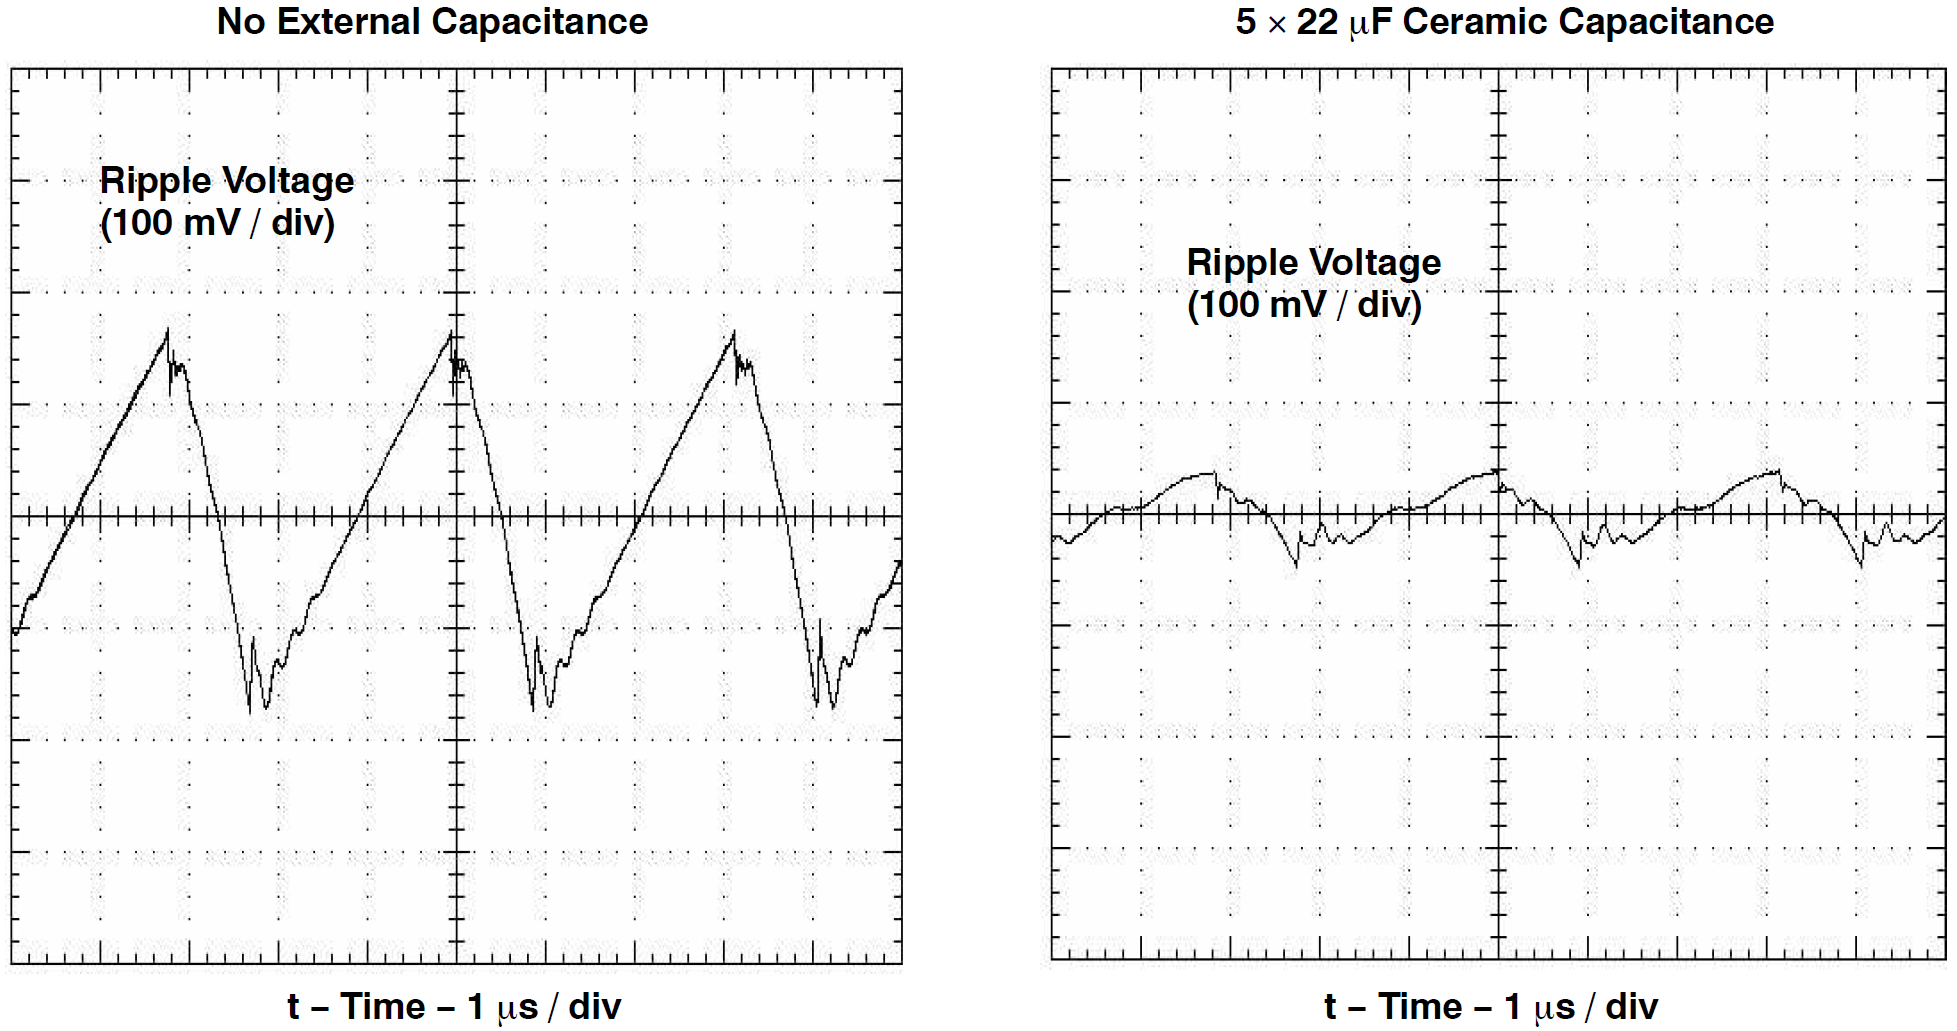
\includegraphics[width=\linewidth]{fig/lec08/input_ripple_voltage_plots.png}
    \caption{Input ripple-voltage reduction after adding ceramic input capacitors. Adapted from Texas Instruments, \textit{Input and Output Capacitor Selection}}
\end{figure}
\end{column}
\end{columns}
The bulk capacitor supports low-frequency energy demand; the local ceramic capacitor handles high-frequency switching current.
\end{frame}


%%%%%%%%%%%%%%%%%%%%%%%%%%%%%%%%%%%%%%%%%%%%%%%%%%%%%%%%%%%%%
%% Output capacitor function
%%%%%%%%%%%%%%%%%%%%%%%%%%%%%%%%%%%%%%%%%%%%%%%%%%%%%%%%%%%%%
\begin{frame}
\frametitle{Output Capacitor in a Buck Converter}

\begin{columns}
\begin{column}{0.56\textwidth}

The output capacitor reduces output-voltage ripple and supplies transient load current until the converter control loop and inductor current can respond. The output ripple contains several components:
\begin{align}
    \Delta v_o
    =
    \Delta v_C
    +
    \Delta v_{\mathrm{ESR}}
    +
    \Delta v_{\mathrm{ESL}}
\end{align}
where
\begin{itemize}
    \item \(\Delta v_C\) is due to charge/discharge of capacitance,
    \item \(\Delta v_{\mathrm{ESR}}\) is due to ripple current through ESR,
    \item \(\Delta v_{\mathrm{ESL}}\) is due to fast current transitions through ESL.
\end{itemize}
\end{column}

\begin{column}{0.40\textwidth}
\begin{figure}
    \centering
    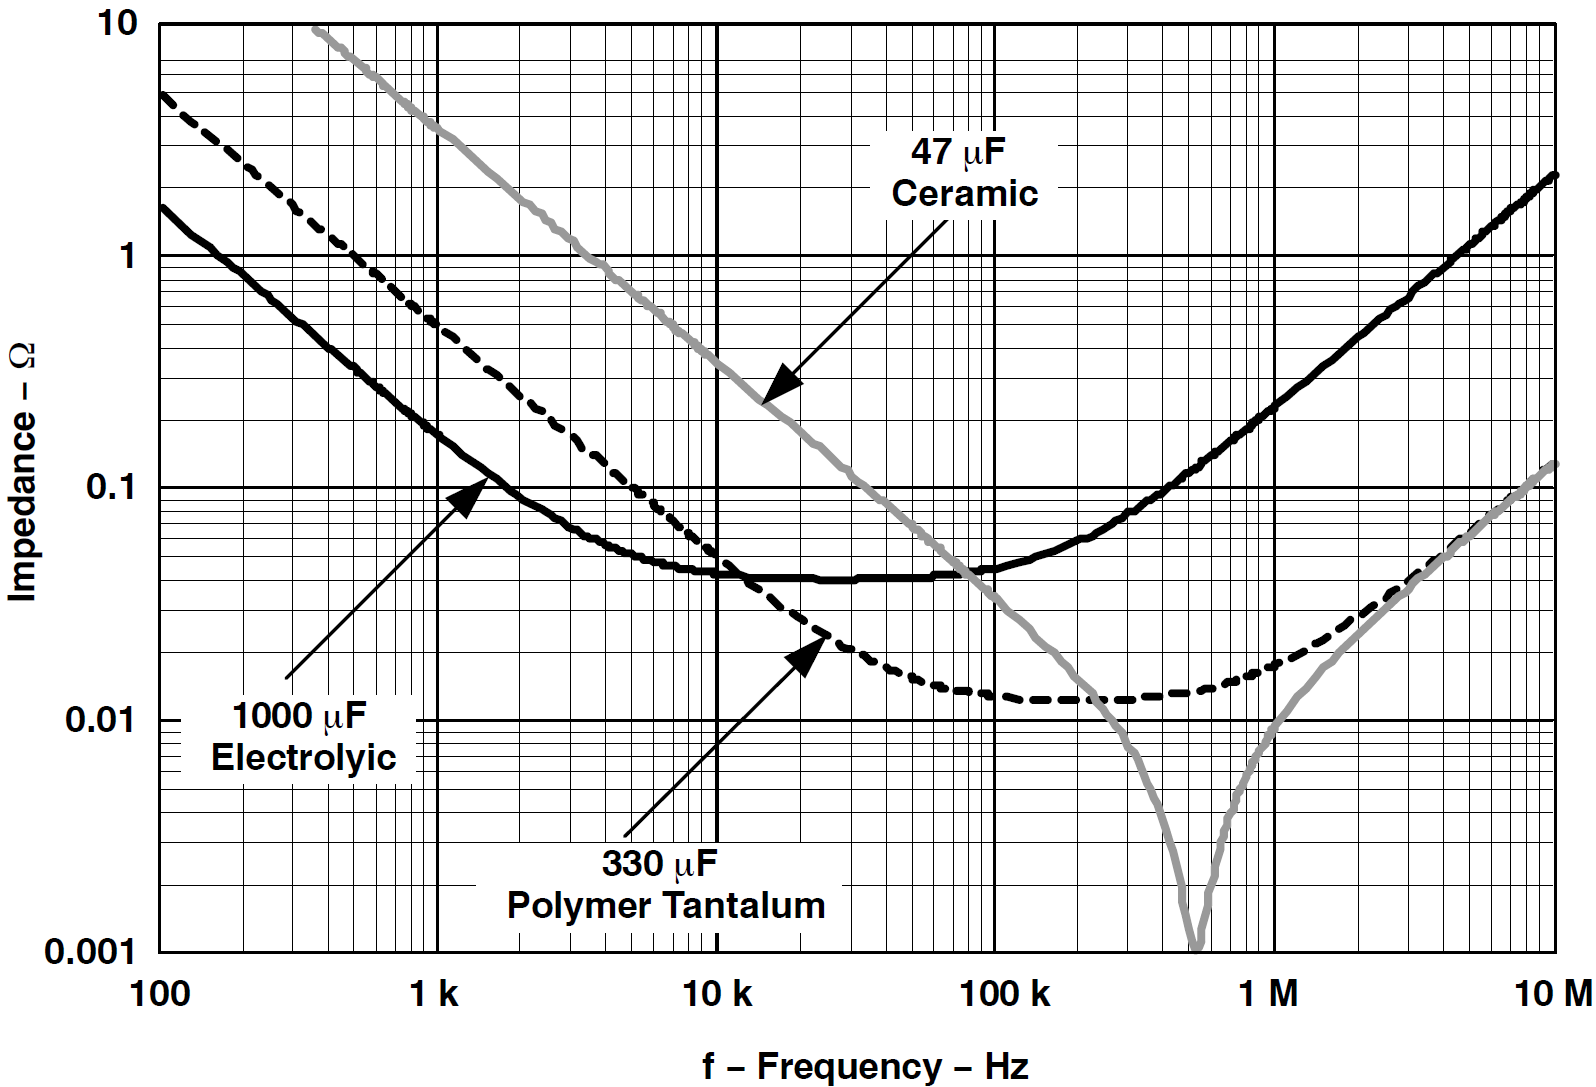
\includegraphics[width=\linewidth]{fig/lec08/capacitor_impedance_characteristics.png}
    \caption{Capacitor impedance characteristics relevant to output capacitor selection. Adapted from Texas Instruments, \textit{Input and Output Capacitor Selection}}
\end{figure}
\end{column}
\end{columns}

\end{frame}

%%%%%%%%%%%%%%%%%%%%%%%%%%%%%%%%%%%%%%%%%%%%%%%%%%%%%%%%%%%%%
%% Output capacitor function
%%%%%%%%%%%%%%%%%%%%%%%%%%%%%%%%%%%%%%%%%%%%%%%%%%%%%%%%%%%%%
\begin{frame}
\frametitle{Output Capacitor in a Buck Converter}

\begin{columns}
\begin{column}{0.56\textwidth}
For inductor ripple current \(\Delta i_L\), the ideal capacitive ripple is approximately
\begin{align}
    \Delta v_C
    \approx
    \frac{\Delta i_L}{8f_sC_o}
\end{align}
for a buck converter with triangular ripple current.
\end{column}

\begin{column}{0.40\textwidth}
\begin{figure}
    \centering
    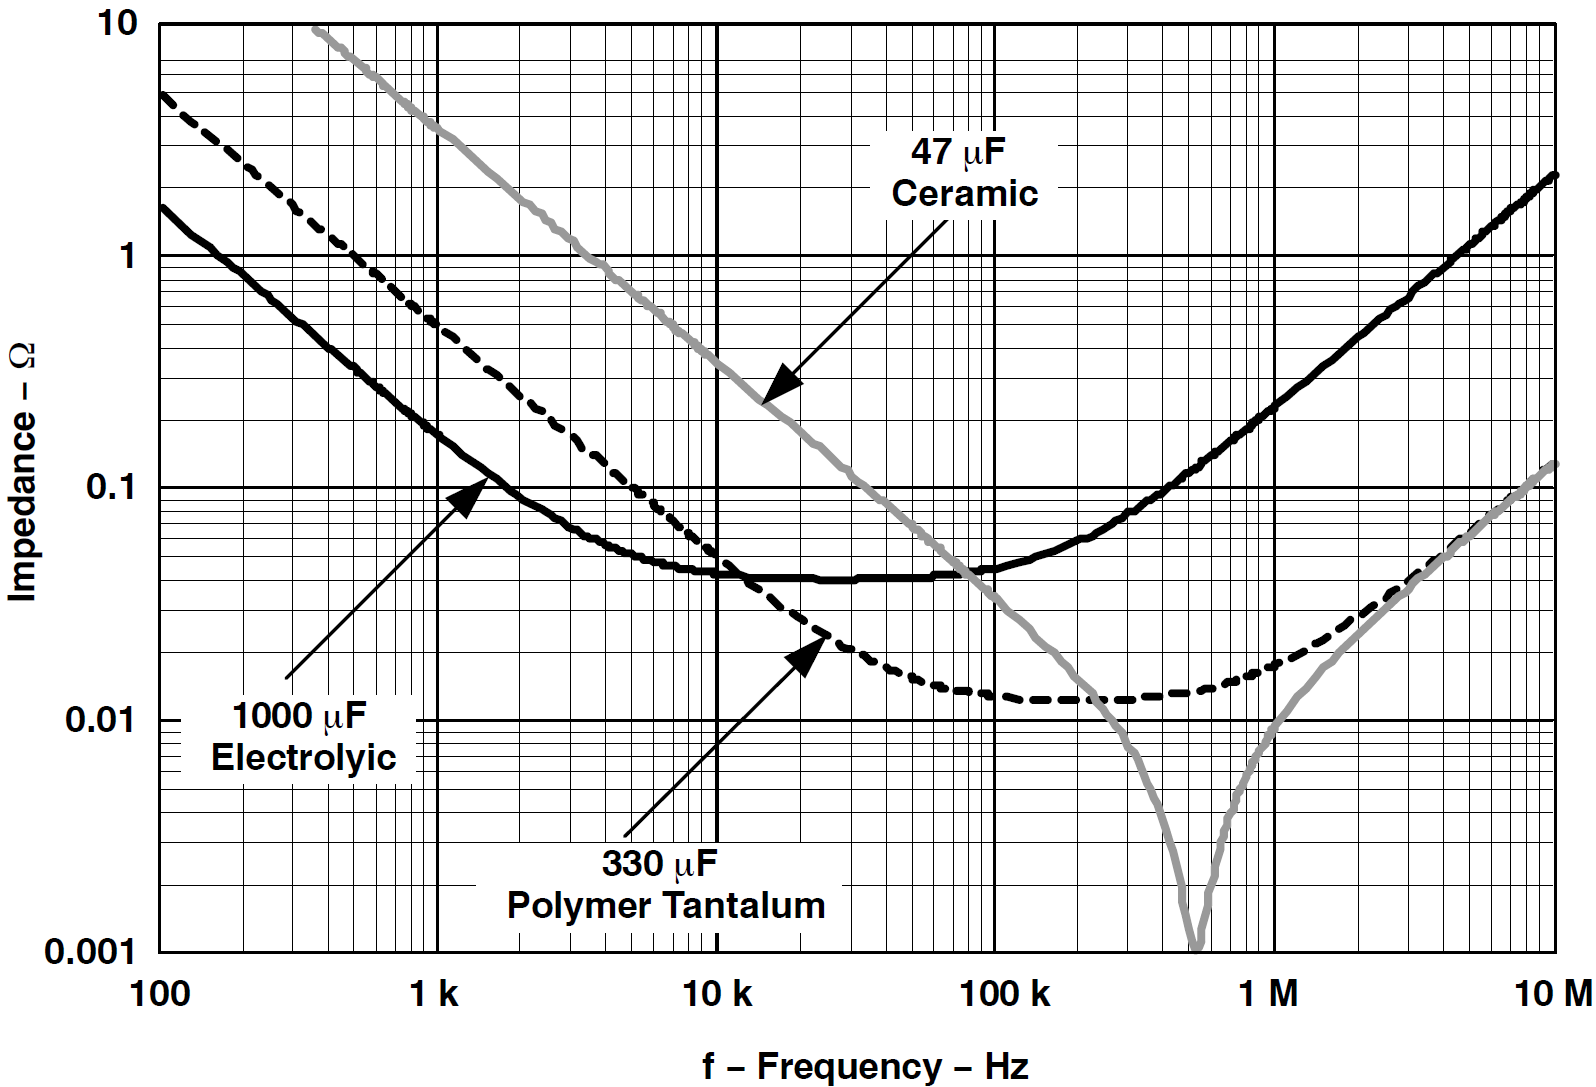
\includegraphics[width=\linewidth]{fig/lec08/capacitor_impedance_characteristics.png}
    \caption{Capacitor impedance characteristics relevant to output capacitor selection. Adapted from Texas Instruments, \textit{Input and Output Capacitor Selection}}
\end{figure}
\end{column}
\end{columns}

\end{frame}

%%%%%%%%%%%%%%%%%%%%%%%%%%%%%%%%%%%%%%%%%%%%%%%%%%%%%%%%%%%%%
%% Output capacitor load transient
%%%%%%%%%%%%%%%%%%%%%%%%%%%%%%%%%%%%%%%%%%%%%%%%%%%%%%%%%%%%%
\begin{frame}
\frametitle{Output Capacitor During Load Transients}
\begin{columns}
\begin{column}{0.56\textwidth}
During a sudden load-current increase, the converter inductor current cannot change instantaneously. The maximum inductor current slew rate is limited by
\begin{align}
    \frac{di_L}{dt}
    =
    \frac{\Delta V_L}{L}
\end{align}
Until the inductor current reaches the new load current, the current deficit must be supplied by the output capacitor. For a fast transient, the first voltage drop is often dominated by ESR:
\begin{align}
    \Delta V_{\mathrm{ESR}}
    =
    \Delta I_{\mathrm{load}} R_{\mathrm{ESR,eq}}
\end{align}
For slower transients, capacitance and control-loop response also contribute. Therefore, output capacitor design is a combination of impedance, capacitance, ESR, ESL, and control-loop bandwidth.
\end{column}

\begin{column}{0.40\textwidth}
\begin{figure}
    \centering
    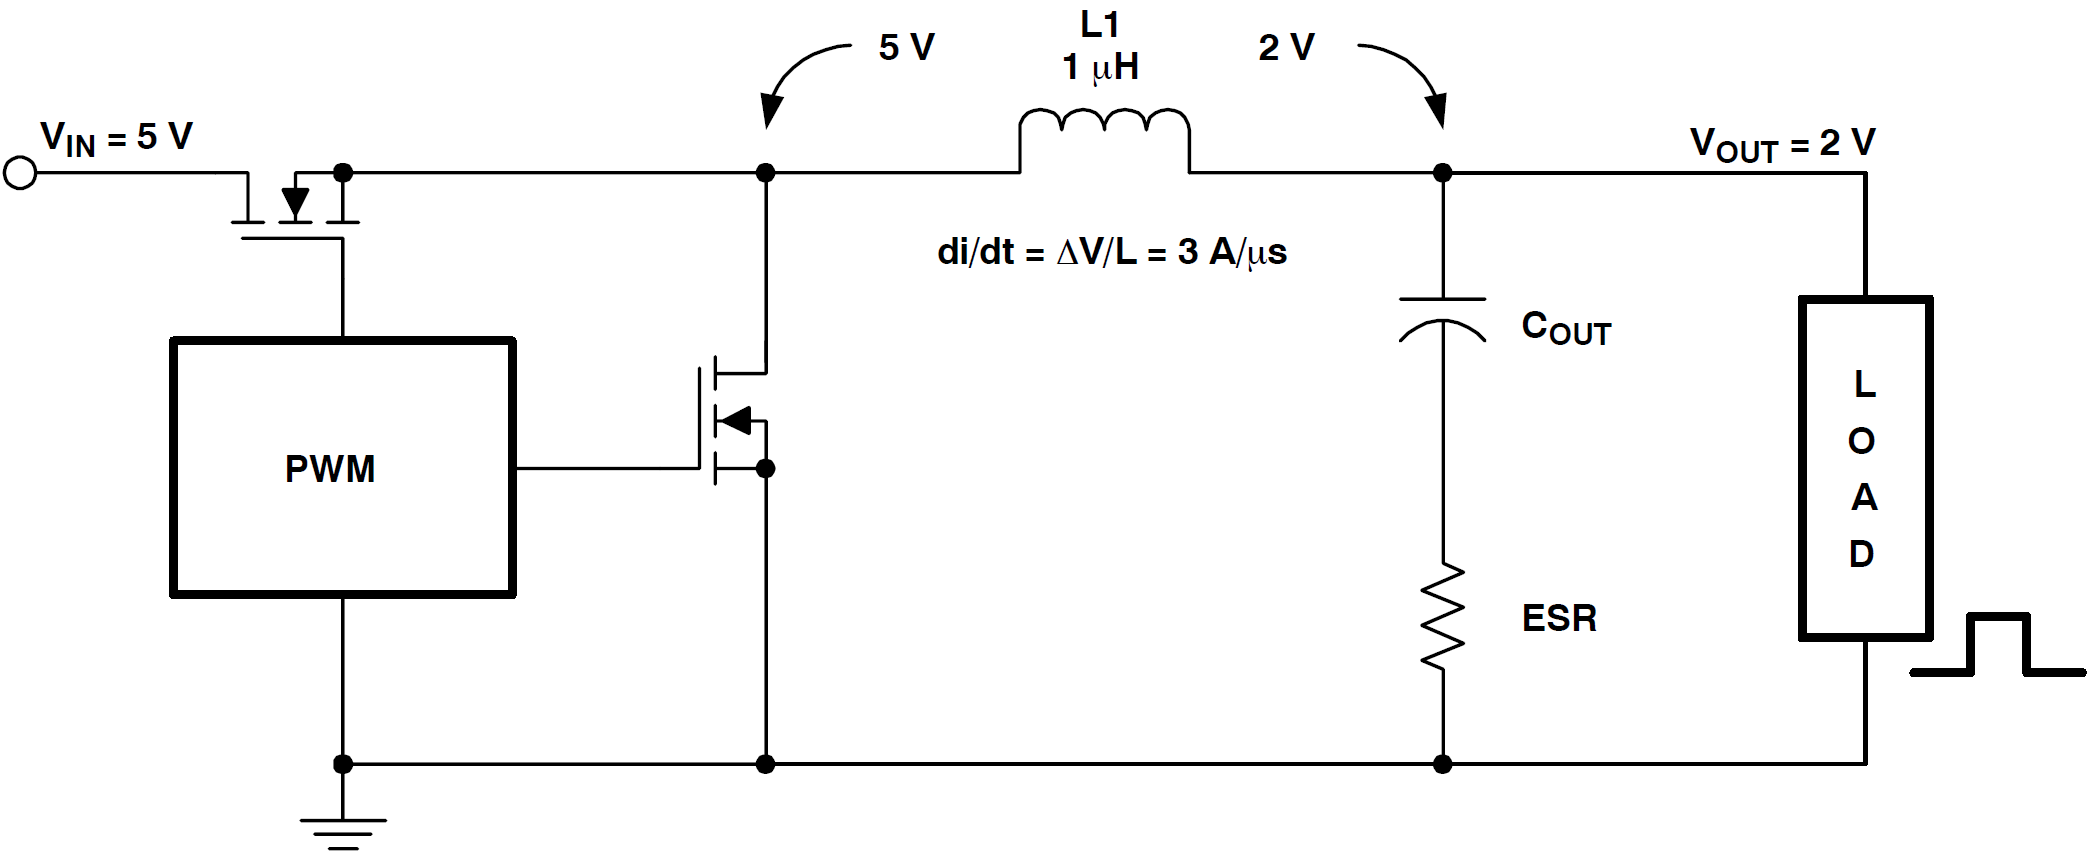
\includegraphics[width=\linewidth]{fig/lec08/regulator_slew_rate_example.png}
    \caption{Buck regulator slew-rate limitation during a load transient. Adapted from Texas Instruments, \textit{Input and Output Capacitor Selection}}
\end{figure}
\end{column}
\end{columns}

\end{frame}


%%%%%%%%%%%%%%%%%%%%%%%%%%%%%%%%%%%%%%%%%%%%%%%%%%%%%%%%%%%%%
%% Target impedance
%%%%%%%%%%%%%%%%%%%%%%%%%%%%%%%%%%%%%%%%%%%%%%%%%%%%%%%%%%%%%
\begin{frame}
\frametitle{Target Impedance for Output Capacitor Networks}
\begin{columns}
\begin{column}{0.56\textwidth}
A practical way to design output decoupling is the target-impedance method. For a maximum allowable transient voltage deviation \(\Delta V_{\max}\) and load step \(\Delta I_{\mathrm{load}}\),
\begin{align}
    Z_{\max}
    =
    \frac{\Delta V_{\max}}
    {\Delta I_{\mathrm{load}}}
\end{align}
The capacitor network should maintain
\begin{align}
    |Z_{\mathrm{out}}(j\omega)| < Z_{\max}
\end{align}
over the frequency range where the regulator cannot respond quickly enough. 
\end{column}

\begin{column}{0.40\textwidth}
\begin{figure}
    \centering
    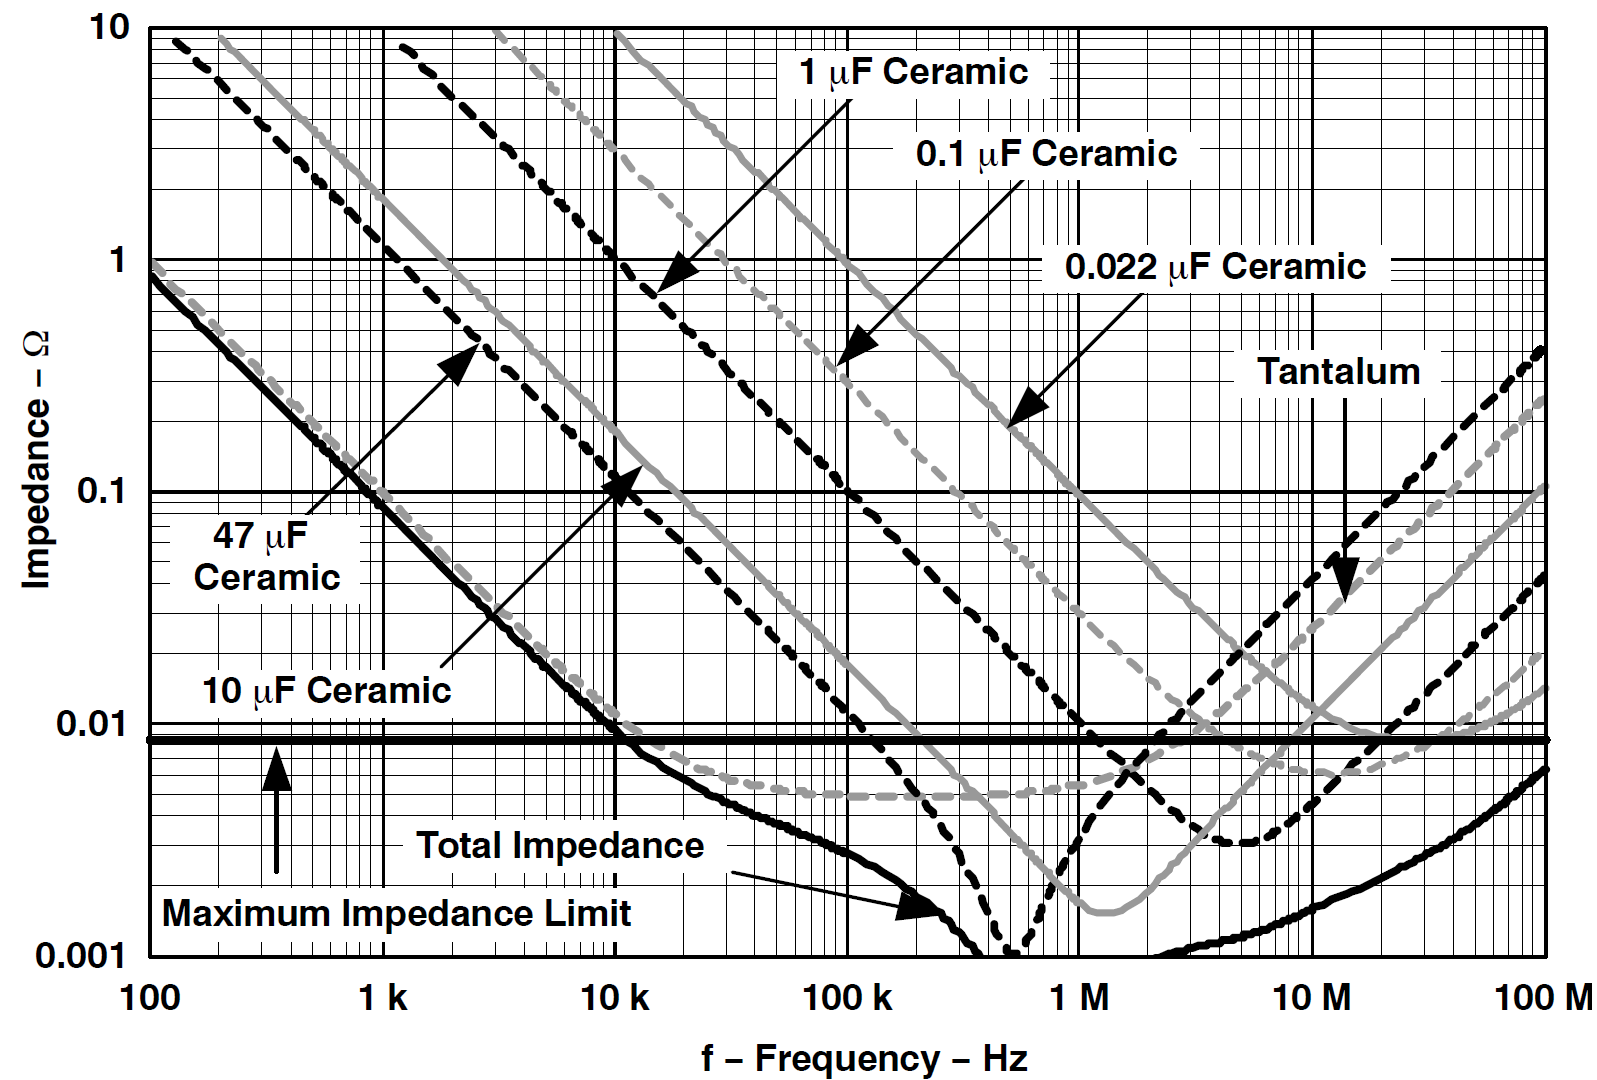
\includegraphics[width=\linewidth]{fig/lec08/high_frequency_impedance_plot.png}
    \caption{Output capacitor network impedance using multiple capacitor values and technologies. Adapted from Texas Instruments, \textit{Input and Output Capacitor Selection}}
\end{figure}
\end{column}
\end{columns}

\end{frame}


%%%%%%%%%%%%%%%%%%%%%%%%%%%%%%%%%%%%%%%%%%%%%%%%%%%%%%%%%%%%%
%% Target impedance
%%%%%%%%%%%%%%%%%%%%%%%%%%%%%%%%%%%%%%%%%%%%%%%%%%%%%%%%%%%%%
\begin{frame}
\frametitle{Target Impedance for Output Capacitor Networks}
\begin{columns}
\begin{column}{0.56\textwidth}
This usually requires several capacitor types:
\begin{itemize}
    \item bulk capacitor for low frequency,
    \item polymer or film capacitor for mid-frequency,
    \item MLCCs for high-frequency transients,
    \item very small MLCCs for MHz-range local decoupling.
\end{itemize}
\end{column}

\begin{column}{0.40\textwidth}
\begin{figure}
    \centering
    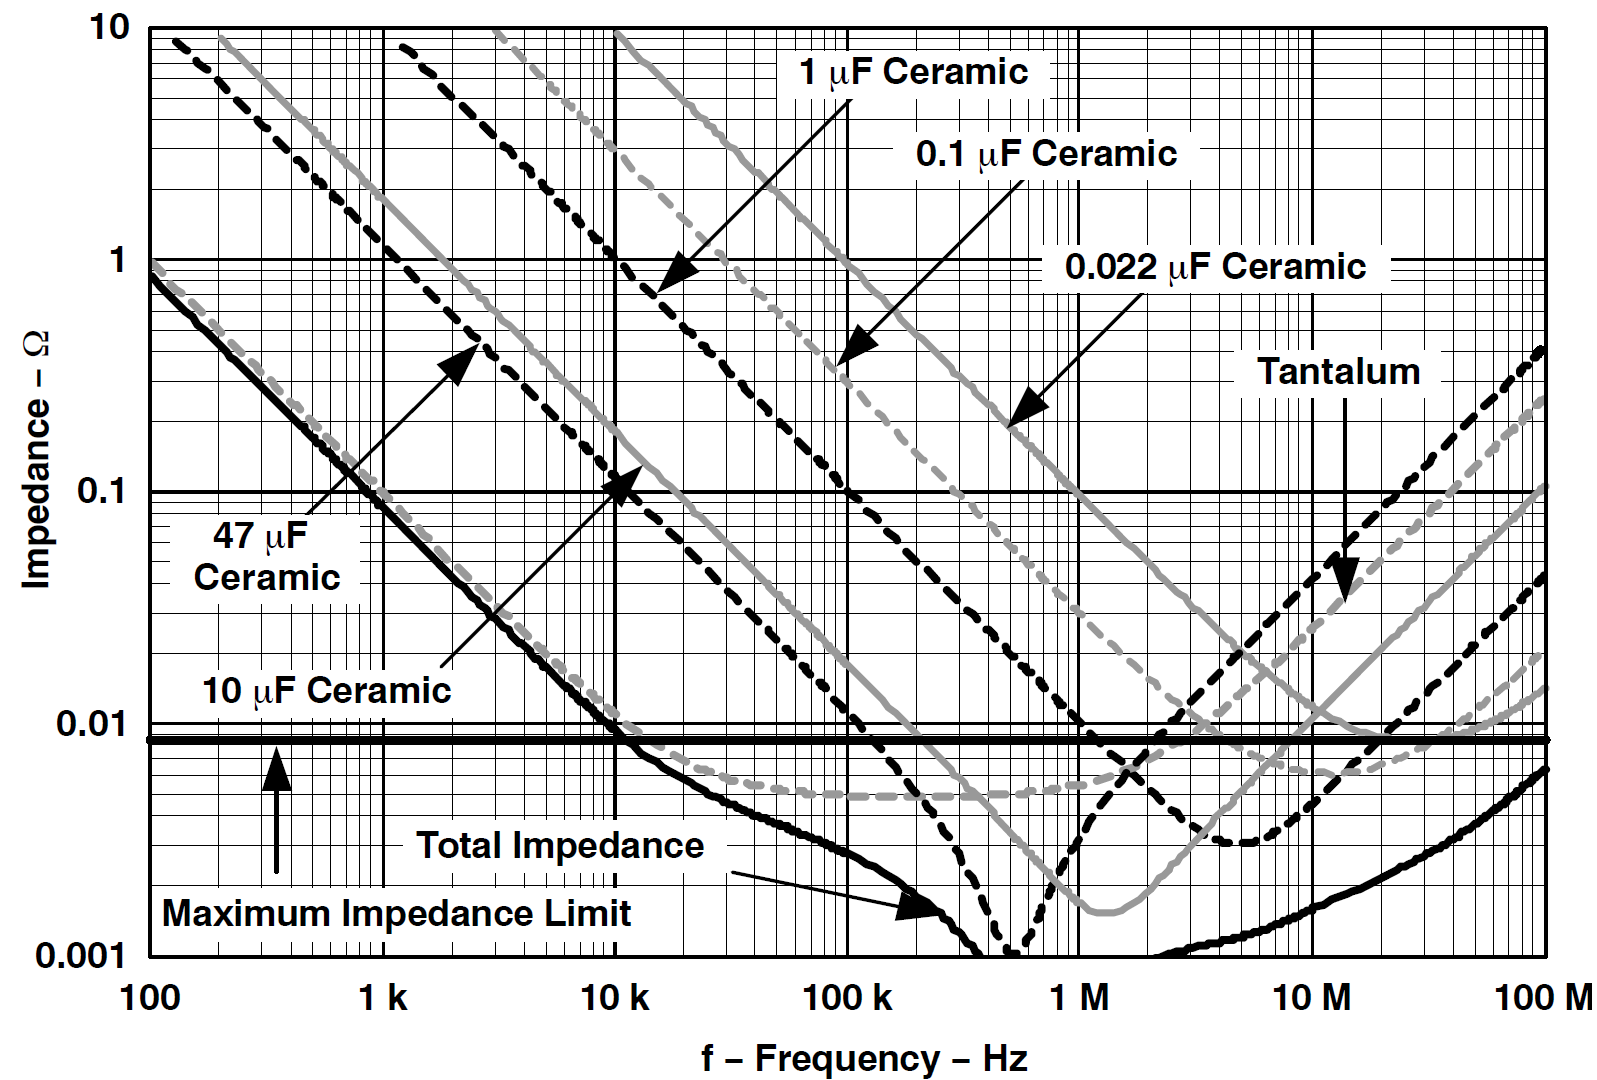
\includegraphics[width=\linewidth]{fig/lec08/high_frequency_impedance_plot.png}
    \caption{Output capacitor network impedance using multiple capacitor values and technologies. Adapted from Texas Instruments, \textit{Input and Output Capacitor Selection}}
\end{figure}
\end{column}
\end{columns}

\end{frame}
%%%%%%%%%%%%%%%%%%%%%%%%%%%%%%%%%%%%%%%%%%%%%%%%%%%%%%%%%%%%%
%% DC-link capacitor
%%%%%%%%%%%%%%%%%%%%%%%%%%%%%%%%%%%%%%%%%%%%%%%%%%%%%%%%%%%%%
\begin{frame}
\frametitle{DC-Link Capacitor}
\begin{columns}
\begin{column}{0.56\textwidth}
The DC-link capacitor is placed between two converter stages, for example between a rectifier and an inverter. Its main functions are:
\begin{itemize}
    \item balance instantaneous power between source and load,
    \item limit DC-bus voltage ripple,
    \item provide transient energy storage,
    \item reduce interaction between converter stages,
    \item provide a low-impedance path for switching ripple current.
\end{itemize}
\end{column}

\begin{column}{0.40\textwidth}
\begin{figure}
    \centering
    \vspace{-0.5cm}
    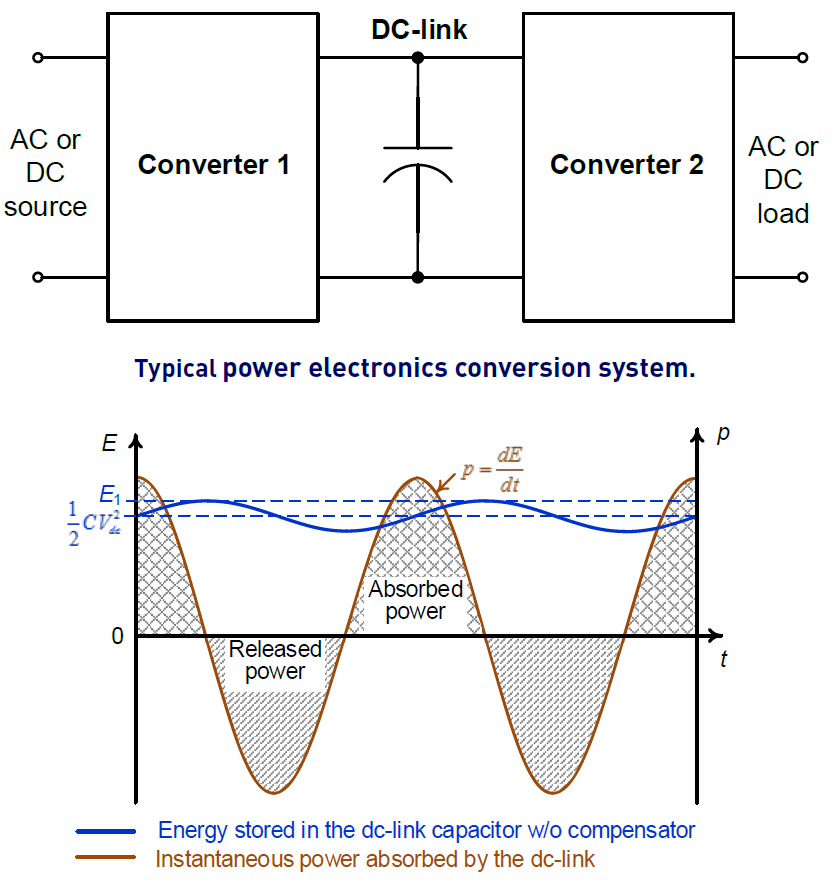
\includegraphics[width=0.75\linewidth]{fig/lec08/DC_link_function.png}
    \caption{Function of a capacitive DC link: power balancing, voltage-ripple limitation, and energy storage. Adapted from Huai Wang, \textit{Capacitors in Power Electronics Applications -- Reliability and Circuit Design}, IECON 2016 tutorial}
\end{figure}
\end{column}
\end{columns}
\end{frame}


%%%%%%%%%%%%%%%%%%%%%%%%%%%%%%%%%%%%%%%%%%%%%%%%%%%%%%%%%%%%%
%% DC-link capacitor
%%%%%%%%%%%%%%%%%%%%%%%%%%%%%%%%%%%%%%%%%%%%%%%%%%%%%%%%%%%%%
\begin{frame}
\frametitle{DC-Link Capacitor}
\begin{columns}
\begin{column}{0.56\textwidth}
The DC-link capacitor stored energy is
\begin{align}
    E_{\mathrm{dc}}
    =
    \frac{1}{2}C_{\mathrm{dc}}V_{\mathrm{dc}}^2
\end{align}
A small change in DC-link voltage corresponds to an energy change:
\begin{align}
    \Delta E
    =
    \frac{1}{2}C_{\mathrm{dc}}
    \left(
    V_{\max}^2 - V_{\min}^2
    \right)
\end{align}
\end{column}

\begin{column}{0.40\textwidth}
\begin{figure}
    \centering
    \vspace{-0.5cm}
    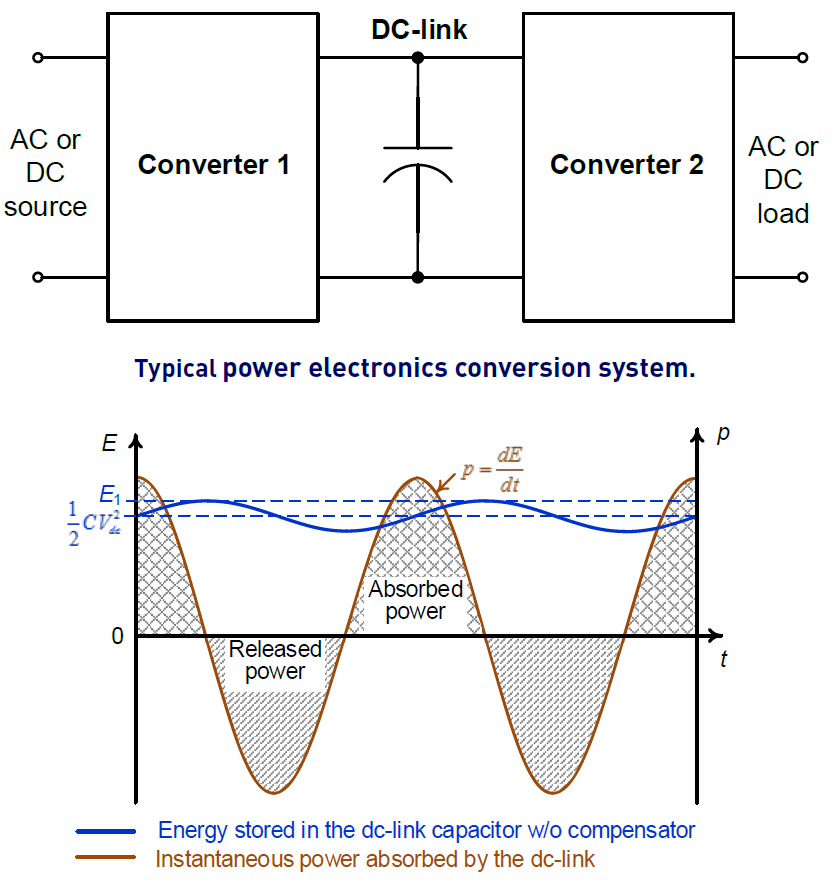
\includegraphics[width=0.75\linewidth]{fig/lec08/DC_link_function.png}
    \caption{Function of a capacitive DC link: power balancing, voltage-ripple limitation, and energy storage. Adapted from Huai Wang, \textit{Capacitors in Power Electronics Applications -- Reliability and Circuit Design}, IECON 2016 tutorial}
\end{figure}
\end{column}
\end{columns}
\end{frame}

%%%%%%%%%%%%%%%%%%%%%%%%%%%%%%%%%%%%%%%%%%%%%%%%%%%%%%%%%%%%%
%% DC-link capacitor in inverter
%%%%%%%%%%%%%%%%%%%%%%%%%%%%%%%%%%%%%%%%%%%%%%%%%%%%%%%%%%%%%
\begin{frame}
\frametitle{DC-Link Capacitor in Inverters and Motor Drives}
\begin{columns}
\begin{column}{0.56\textwidth}
In inverter systems, the DC-link capacitor is exposed to both low-frequency and high-frequency stress. Typical stress components include:
\begin{itemize}
    \item rectifier-side ripple,
    \item inverter switching ripple,
    \item load-dependent RMS ripple current,
    \item regenerative braking energy,
    \item overvoltage during load transients,
    \item thermal cycling from mission-profile variation.
\end{itemize}
\end{column}

\begin{column}{0.40\textwidth}
\begin{figure}
    \centering
    \vspace{-0.5cm}
    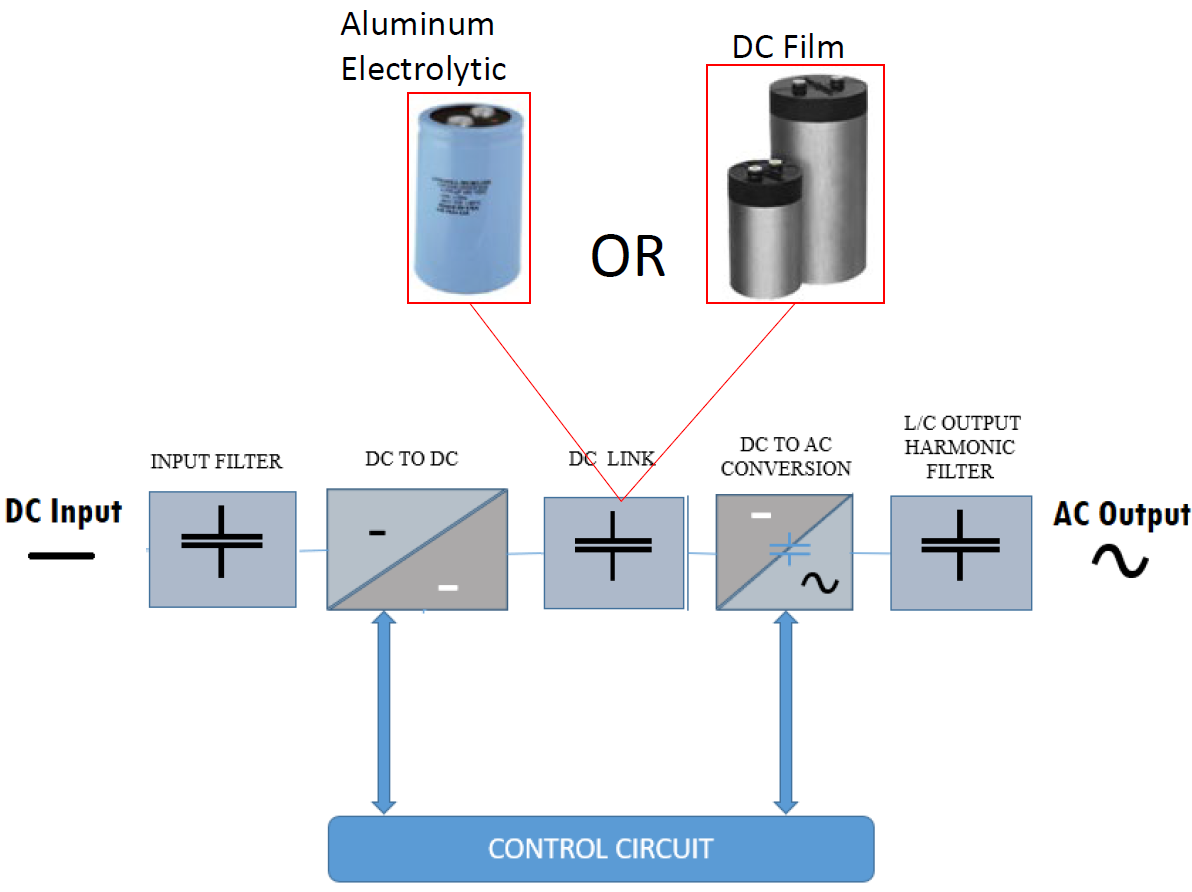
\includegraphics[width=\linewidth]{fig/lec08/DC_link_capacitors.png}
    \caption{DC-link capacitor location in a high-power inverter/converter system. Adapted from Cornell Dubilier, \textit{Capacitors for High Power Inverters and Converters}}
\end{figure}
\end{column}
\end{columns}

\end{frame}


%%%%%%%%%%%%%%%%%%%%%%%%%%%%%%%%%%%%%%%%%%%%%%%%%%%%%%%%%%%%%
%% DC-link capacitor in inverter
%%%%%%%%%%%%%%%%%%%%%%%%%%%%%%%%%%%%%%%%%%%%%%%%%%%%%%%%%%%%%
\begin{frame}
\frametitle{DC-Link Capacitor in Inverters and Motor Drives}
\begin{columns}
\begin{column}{0.56\textwidth}
For motor drives and grid converters, the DC-link capacitor is often one of the lifetime-critical components. Technology choice:
\begin{itemize}
    \item aluminum electrolytic: high capacitance and lower cost,
    \item film: higher ripple current, lower ESR, longer life, non-polar operation.
\end{itemize}
\end{column}

\begin{column}{0.40\textwidth}
\begin{figure}
    \centering
    \vspace{-0.5cm}
    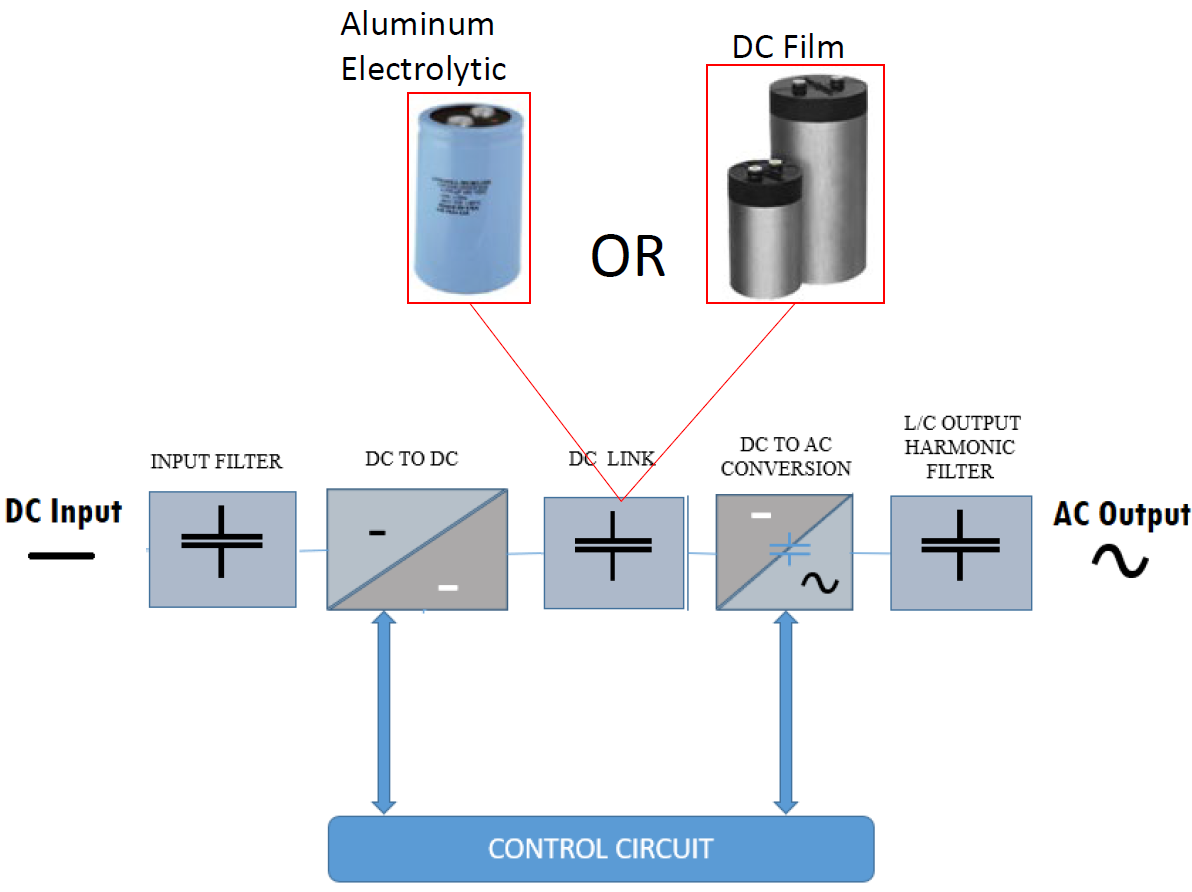
\includegraphics[width=\linewidth]{fig/lec08/DC_link_capacitors.png}
    \caption{DC-link capacitor location in a high-power inverter/converter system. Adapted from Cornell Dubilier, \textit{Capacitors for High Power Inverters and Converters}}
\end{figure}
\end{column}
\end{columns}

\end{frame}

%%%%%%%%%%%%%%%%%%%%%%%%%%%%%%%%%%%%%%%%%%%%%%%%%%%%%%%%%%%%%
%% Snubber capacitor
%%%%%%%%%%%%%%%%%%%%%%%%%%%%%%%%%%%%%%%%%%%%%%%%%%%%%%%%%%%%%
\begin{frame}
\frametitle{Snubber Capacitor}
\begin{columns}
\begin{column}{0.56\textwidth}
A snubber capacitor limits switching overvoltage caused by stray inductance:
\begin{align}
    v_{\mathrm{transient}}
    =
    L_{\sigma}\frac{di}{dt}
\end{align}
where \(L_{\sigma}\) is the commutation-loop stray inductance. It provides a local switching-current path and reduces device voltage rise. Key requirements:
\begin{itemize}
    \item low ESL,
    \item high pulse-current capability,
    \item high \(dv/dt\) rating,
    \item low loss at switching frequency,
    \item high voltage rating and surge capability.
\end{itemize}

\end{column}

\begin{column}{0.40\textwidth}
\begin{figure}
    \centering
    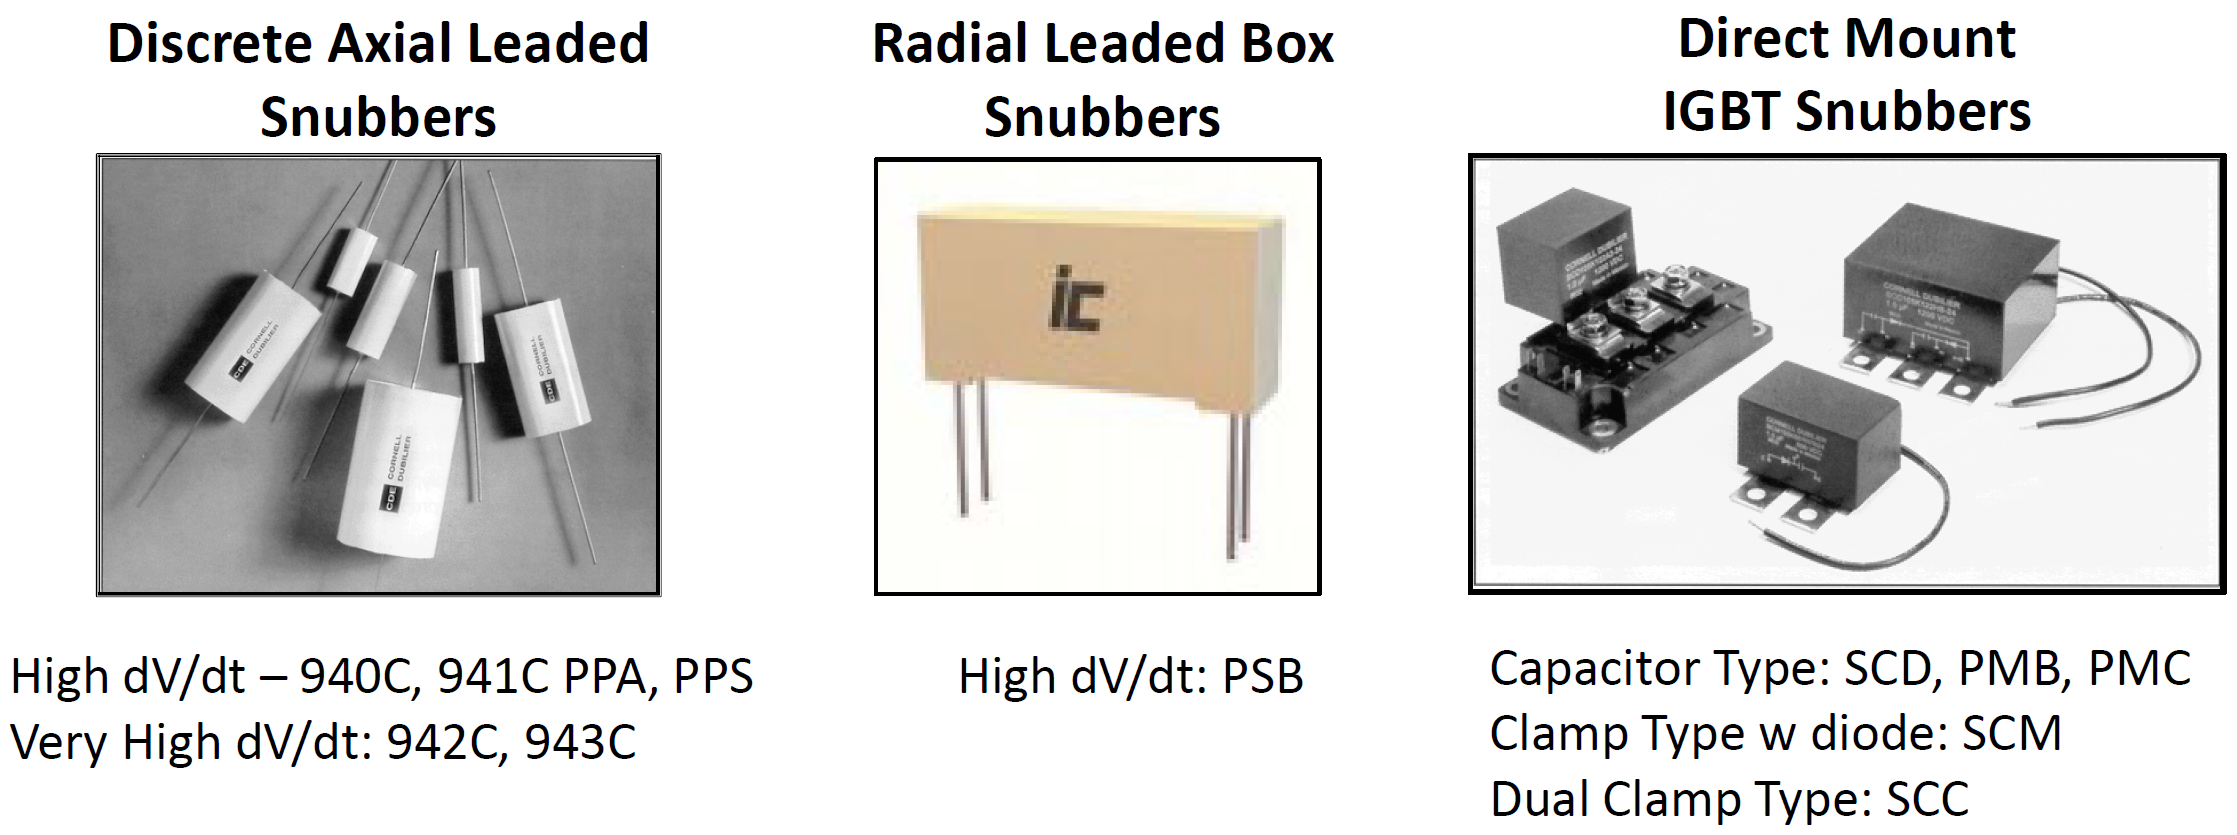
\includegraphics[width=\linewidth]{fig/lec08/snubber_definition_slide.png}
    \caption{Snubber concept: protection of switching devices from turn-off overvoltage caused by stray inductance and fast current change. Adapted from Cornell Dubilier, \textit{Capacitors for High Power Inverters and Converters}}
\end{figure}
\end{column}
\end{columns}

\end{frame}


%%%%%%%%%%%%%%%%%%%%%%%%%%%%%%%%%%%%%%%%%%%%%%%%%%%%%%%%%%%%%
%% Snubber voltage waveform
%%%%%%%%%%%%%%%%%%%%%%%%%%%%%%%%%%%%%%%%%%%%%%%%%%%%%%%%%%%%%
\begin{frame}
\frametitle{Snubber Capacitor Voltage Stress}
\begin{columns}
\begin{column}{0.56\textwidth}
Snubber capacitors require verification of voltage waveform, peak current, RMS current, and \(dv/dt\) rating. The capacitor current is
\begin{align}
    i_C = C\frac{dv_C}{dt}
\end{align}
High \(dv/dt\) produces high pulse current. For repetitive duty, verify:
\begin{itemize}
    \item maximum peak voltage,
    \item repetitive peak current,
    \item RMS current,
    \item pulse energy and thermal rise,
    \item permissible \(dv/dt\),
    \item mounting inductance.
\end{itemize}
\end{column}

\begin{column}{0.40\textwidth}
\begin{block}{Message}
Film capacitors are commonly used because of low loss, self-healing, and high pulse-current capability.
\end{block}
\begin{figure}
    \centering
    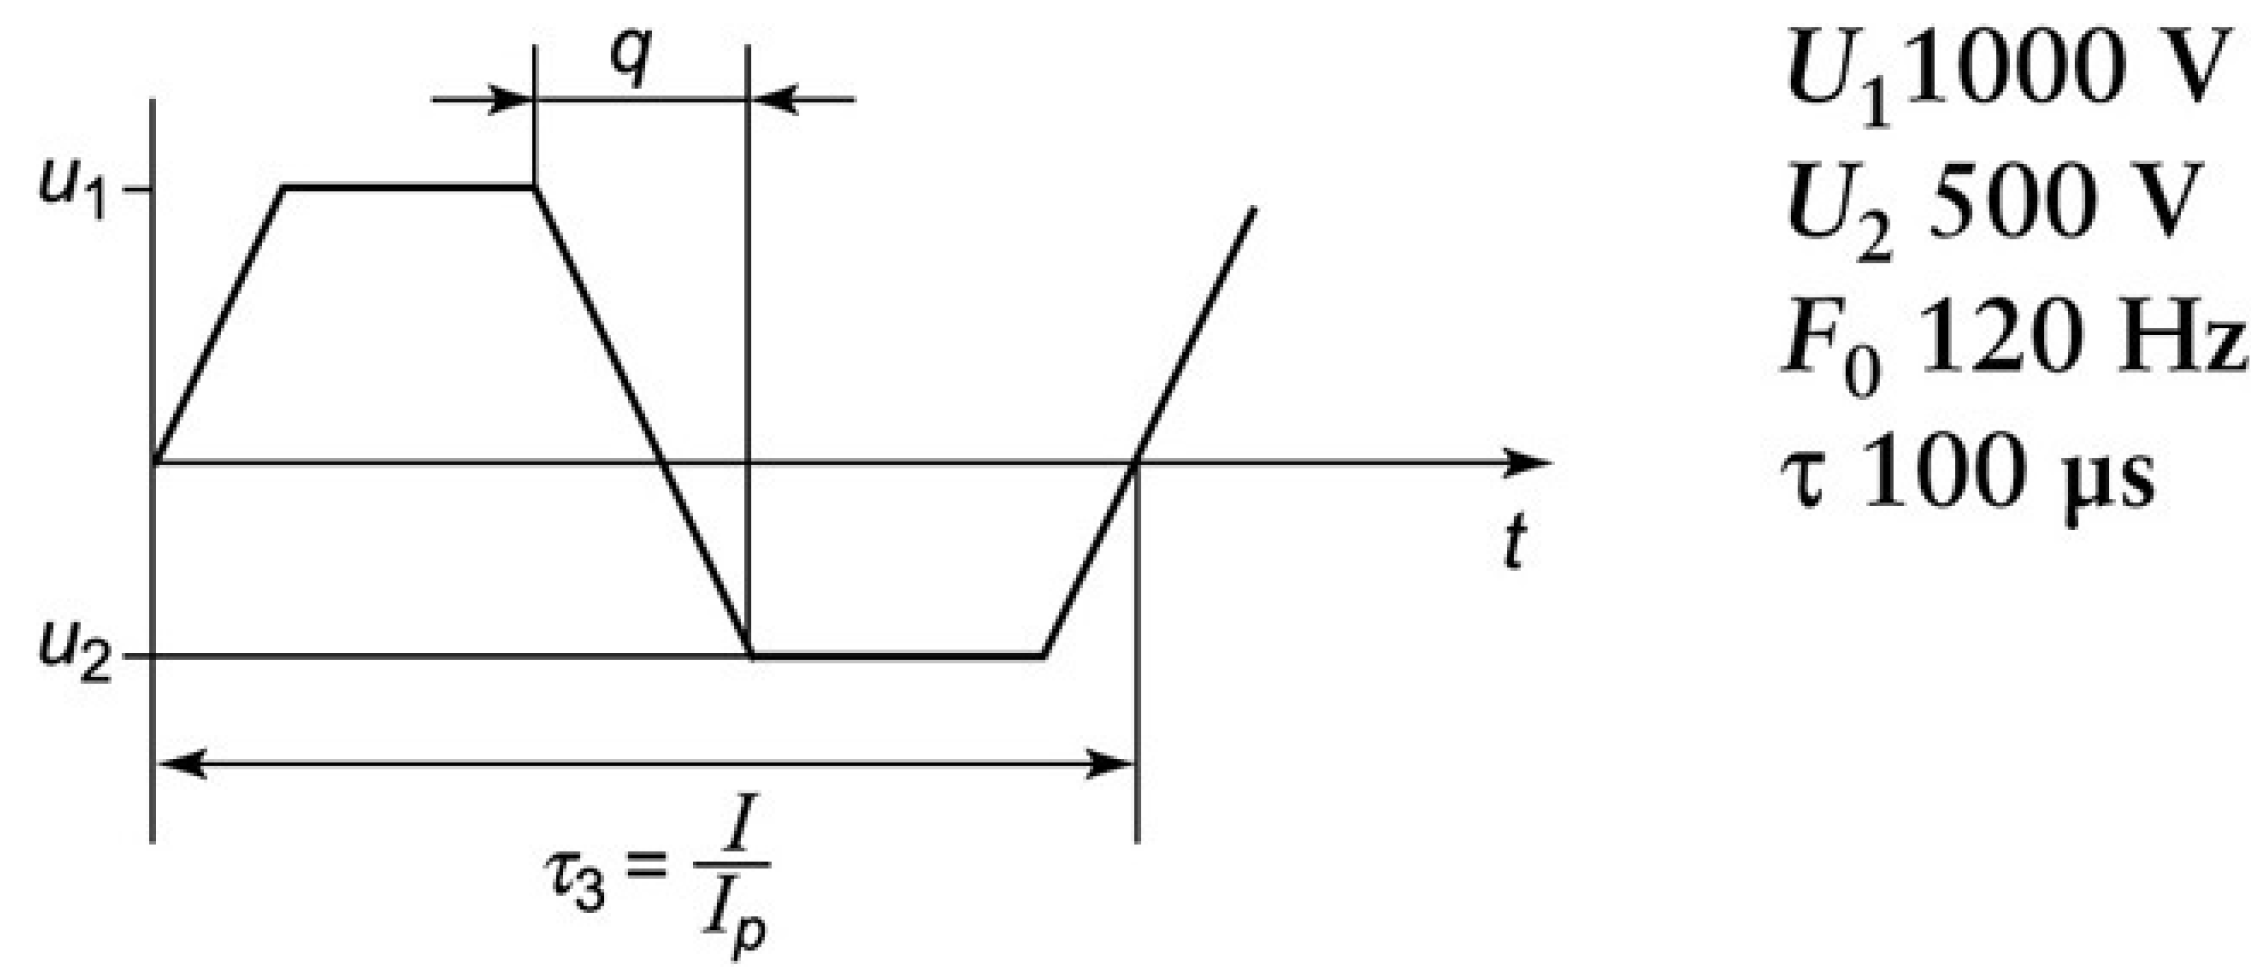
\includegraphics[width=\linewidth]{fig/lec08/snubber_turn_off_waveform.png}
    \caption{Turn-off voltage waveform used for snubber capacitor voltage-stress selection. Adapted from Deshpande, \textit{Capacitors} McGraw-Hill, 2015.}
\end{figure}
\end{column}
\end{columns}

\end{frame}


%%%%%%%%%%%%%%%%%%%%%%%%%%%%%%%%%%%%%%%%%%%%%%%%%%%%%%%%%%%%%
%% Resonant capacitor
%%%%%%%%%%%%%%%%%%%%%%%%%%%%%%%%%%%%%%%%%%%%%%%%%%%%%%%%%%%%%
\begin{frame}
\frametitle{Resonant Capacitor}
\begin{columns}
\begin{column}{0.56\textwidth}
In resonant converters, the capacitor is not only a filter element; it is part of the power-transfer mechanism. For an ideal series resonant tank,
\begin{align}
    f_r
    =
    \frac{1}{2\pi\sqrt{L_rC_r}}
\end{align}
The resonant capacitor must withstand:
\begin{itemize}
    \item high RMS current,
    \item sinusoidal or quasi-sinusoidal AC voltage,
    \item high reactive power circulation,
    \item frequency-dependent dielectric loss,
    \item capacitance tolerance and temperature drift.
\end{itemize}

\end{column}

\begin{column}{0.40\textwidth}
\centering
\begin{circuitikz}[scale=0.82, transform shape]
    \draw (0,0) to[sV,l=$v_{\mathrm{sw}}$] (0,-2.4)
          -- (4.2,-2.4)
          to[C,l=$C_r$] (4.2,-1.2)
          to[L,l=$L_r$] (4.2,0)
          -- (0,0);

    \draw[->, thick] (2.0,0.35) -- (3.4,0.35);
    \node at (2.7,0.68) {\small $i_r$};

    \node at (2.2,-3.0) {\small Simplified series resonant tank};
\end{circuitikz}

\begin{block}{Design Message}
In resonant converters, capacitor stability and loss directly affect resonant frequency, gain curve, circulating current, efficiency, and thermal stress.
\end{block}
\end{column}
\end{columns}
Typical technologies include polypropylene film capacitors, high-quality ceramic capacitors, and specialized resonant capacitors.
\end{frame}


%%%%%%%%%%%%%%%%%%%%%%%%%%%%%%%%%%%%%%%%%%%%%%%%%%%%%%%%%%%%%
%% AC harmonic filter capacitors
%%%%%%%%%%%%%%%%%%%%%%%%%%%%%%%%%%%%%%%%%%%%%%%%%%%%%%%%%%%%%
\begin{frame}
\frametitle{AC Harmonic Filter Capacitors}

\begin{columns}
\begin{column}{0.56\textwidth}
Inverters generate switching-frequency harmonics that must often be attenuated before the grid, motor, or load. AC harmonic filter capacitors are used together with inductors to form:
\begin{itemize}
    \item LC filters and LCL grid filters,
    \item tuned harmonic filters,
    \item motor-output sine filters,
    \item differential-mode EMI filters.
\end{itemize}
The capacitor must be selected for:
\begin{itemize}
    \item RMS voltage and current,
    \item harmonic current spectrum,
    \item dielectric loss and thermal rise,
    \item grid or motor-side overvoltage conditions.
\end{itemize}
\end{column}

\begin{column}{0.40\textwidth}
\begin{figure}
    \centering
    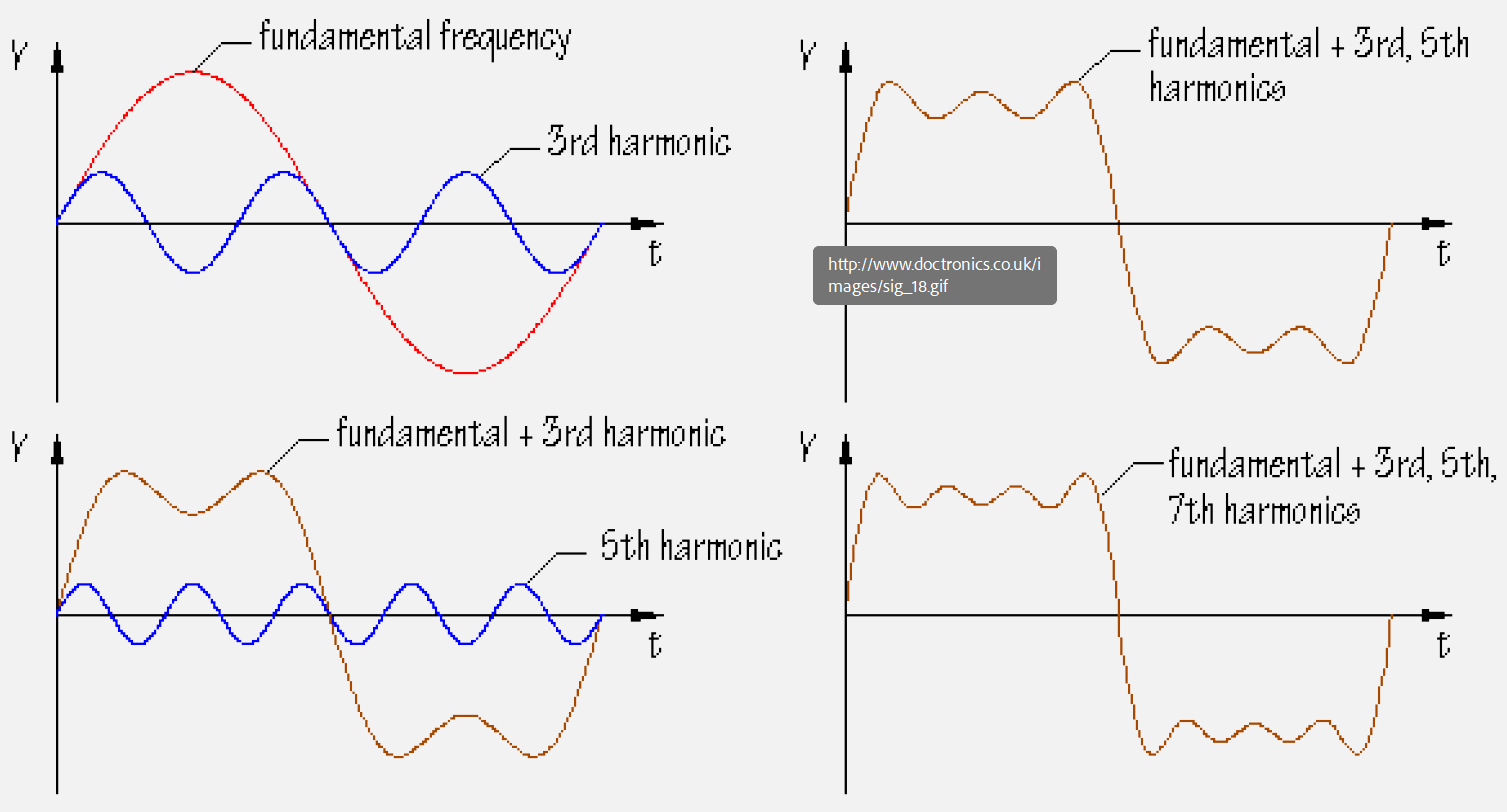
\includegraphics[width=\linewidth]{fig/lec08/AC_harmonic_filtering.png}
    \caption{Inverter switching harmonics and AC harmonic-filter capacitors used with tuned LC networks. Adapted from Cornell Dubilier, \textit{Capacitors for High Power Inverters and Converters}}
\end{figure}
\end{column}
\end{columns}
For AC use, non-polar film capacitors are commonly preferred.
\end{frame}


%%%%%%%%%%%%%%%%%%%%%%%%%%%%%%%%%%%%%%%%%%%%%%%%%%%%%%%%%%%%%
%% EMI and safety capacitors
%%%%%%%%%%%%%%%%%%%%%%%%%%%%%%%%%%%%%%%%%%%%%%%%%%%%%%%%%%%%%
\begin{frame}
\frametitle{EMI and Safety Capacitors}
\begin{columns}
\begin{column}{0.56\textwidth}
Capacitors used in EMI filters must satisfy both electrical and safety requirements.

\textbf{Y capacitors} are connected from line or DC rail to protective earth or chassis:
\begin{itemize}
    \item suppress common-mode noise,
    \item leakage current is safety-critical,
    \item capacitance value is limited by touch-current requirements.
\end{itemize}
\textbf{Y capacitors} are connected from line or DC rail to protective earth or chassis:
\begin{itemize}
    \item suppress common-mode noise,
    \item leakage current is safety-critical,
    \item capacitance value is limited by touch-current requirements.
\end{itemize}
\end{column}

\begin{column}{0.40\textwidth}
\begin{center}
\begin{circuitikz}[scale=0.83, transform shape]
    \draw (0,0) node[left]{L} -- (4,0);
    \draw (0,-1.2) node[left]{N} -- (4,-1.2);
    \draw (0,-2.4) node[left]{PE} -- (4,-2.4);

    \draw (1.3,0) to[C,l=$C_X$] (1.3,-1.2);
    \draw (2.7,0) to[C,l=$C_Y$] (2.7,-2.4);
    \draw (3.5,-1.2) to[C,l=$C_Y$] (3.5,-2.4);

    \node at (2.0,0.45) {\small EMI filter capacitors};
\end{circuitikz}
\end{center}
\end{column}
\end{columns}
\end{frame}



%%%%%%%%%%%%%%%%%%%%%%%%%%%%%%%%%%%%%%%%%%%%%%%%%%%%%%%%%%%%%
%% EMI and safety capacitors
%%%%%%%%%%%%%%%%%%%%%%%%%%%%%%%%%%%%%%%%%%%%%%%%%%%%%%%%%%%%%
\begin{frame}
\frametitle{EMI and Safety Capacitors}
\begin{columns}
\begin{column}{0.56\textwidth}
EMI capacitors are therefore selected not only by capacitance and voltage, but also by safety class, impulse rating, leakage current, and insulation requirements.
\end{column}

\begin{column}{0.40\textwidth}
\begin{figure}
    \centering
    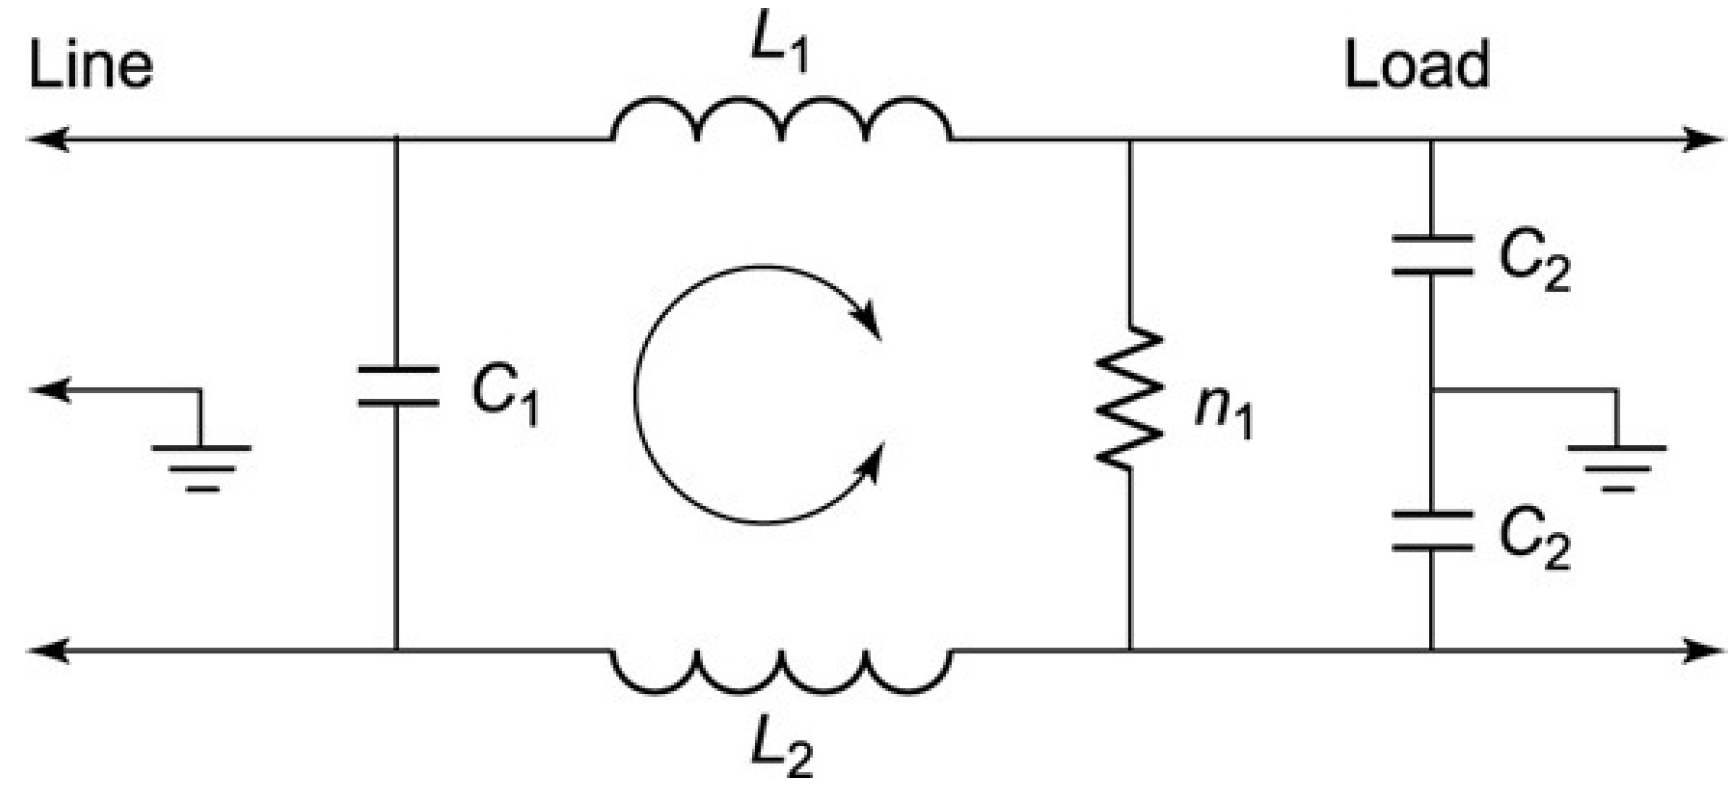
\includegraphics[width=\linewidth]{fig/lec08/XY_capacitors.png}
    \caption{X and Y capacitors used in EMI filters. Adapted from Deshpande, \textit{Capacitors} McGraw-Hill, 2015.}
\end{figure}

\end{column}
\end{columns}
\end{frame}

%%%%%%%%%%%%%%%%%%%%%%%%%%%%%%%%%%%%%%%%%%%%%%%%%%%%%%%%%%%%%
%% Summary of capacitor applications
%%%%%%%%%%%%%%%%%%%%%%%%%%%%%%%%%%%%%%%%%%%%%%%%%%%%%%%%%%%%%
\begin{frame}
\frametitle{Summary: Capacitor Functions in Converters}

\scriptsize
\begin{table}
\centering
\begin{tabular}{p{0.20\textwidth}p{0.25\textwidth}p{0.22\textwidth}p{0.22\textwidth}}
\hline
\textbf{Application} & \textbf{Main Function} & \textbf{Dominant Stress} & \textbf{Typical Technology}\\
\hline
Input capacitor &
Reduce source ripple and supply pulsed current &
High-frequency RMS current, ESL &
MLCC, polymer, electrolytic, film\\

Output capacitor &
Reduce ripple and support load transients &
Target impedance, ESR, transient current &
MLCC, polymer, electrolytic\\

DC-link capacitor &
Energy buffer and DC-bus stabilization &
RMS ripple current, voltage, lifetime &
Film, electrolytic, hybrid banks\\

Snubber capacitor &
Limit switching overvoltage &
High \(dv/dt\), peak current, ESL &
Film, ceramic, power ceramic\\

Resonant capacitor &
Define resonant frequency and transfer power &
High RMS current, low loss, stability &
Polypropylene film, ceramic\\

AC/EMI filter capacitor &
Suppress harmonics and noise &
AC RMS voltage/current, safety &
Film, X/Y safety capacitors\\
\hline
\end{tabular}
\end{table}

\vspace{0.15cm}

\begin{block}{Message}
\small
The capacitor function determines the dominant design constraint. Therefore, the same nominal capacitance value may be suitable in one converter position and completely unsuitable in another.
\end{block}

\end{frame}


%%%%%%%%%%%%%%%%%%%%%%%%%%%%%%%%%%%%%%%%%%%%%%%%%%%%%%%%%%%%%
%% Capacitor sizing and selection methodology
%%%%%%%%%%%%%%%%%%%%%%%%%%%%%%%%%%%%%%%%%%%%%%%%%%%%%%%%%%%%%
\begin{frame}
\begin{center}
  \textbf{\Huge{Capacitor Sizing and Selection}}\\[0.4cm]
  \textbf{\Large{Voltage, Capacitance, Ripple Current, Losses, Temperature, and Layout}}
\end{center}
\end{frame}


%%%%%%%%%%%%%%%%%%%%%%%%%%%%%%%%%%%%%%%%%%%%%%%%%%%%%%%%%%%%%
%% Capacitor selection workflow
%%%%%%%%%%%%%%%%%%%%%%%%%%%%%%%%%%%%%%%%%%%%%%%%%%%%%%%%%%%%%
\begin{frame}
\frametitle{Capacitor Selection Workflow}

\begin{columns}
\begin{column}{0.56\textwidth}
Capacitor selection in power electronics should follow a systematic procedure. The nominal capacitance is only one part of the design. A practical workflow is:

\begin{enumerate}
    \item Define the capacitor function.
    \item Select voltage rating and derating.
    \item Determine required capacitance.
    \item Check RMS and peak current.
    \item Estimate losses and temperature rise.
    \item Verify ESR, ESL and resonance.
    \item Check lifetime and end-of-life limits.
    \item Validate layout, cooling and mechanical mounting.
\end{enumerate}
The final capacitor is acceptable only if all electrical, thermal, reliability and layout constraints are simultaneously satisfied.
\end{column}

\begin{column}{0.40\textwidth}
\begin{figure}
    \centering
    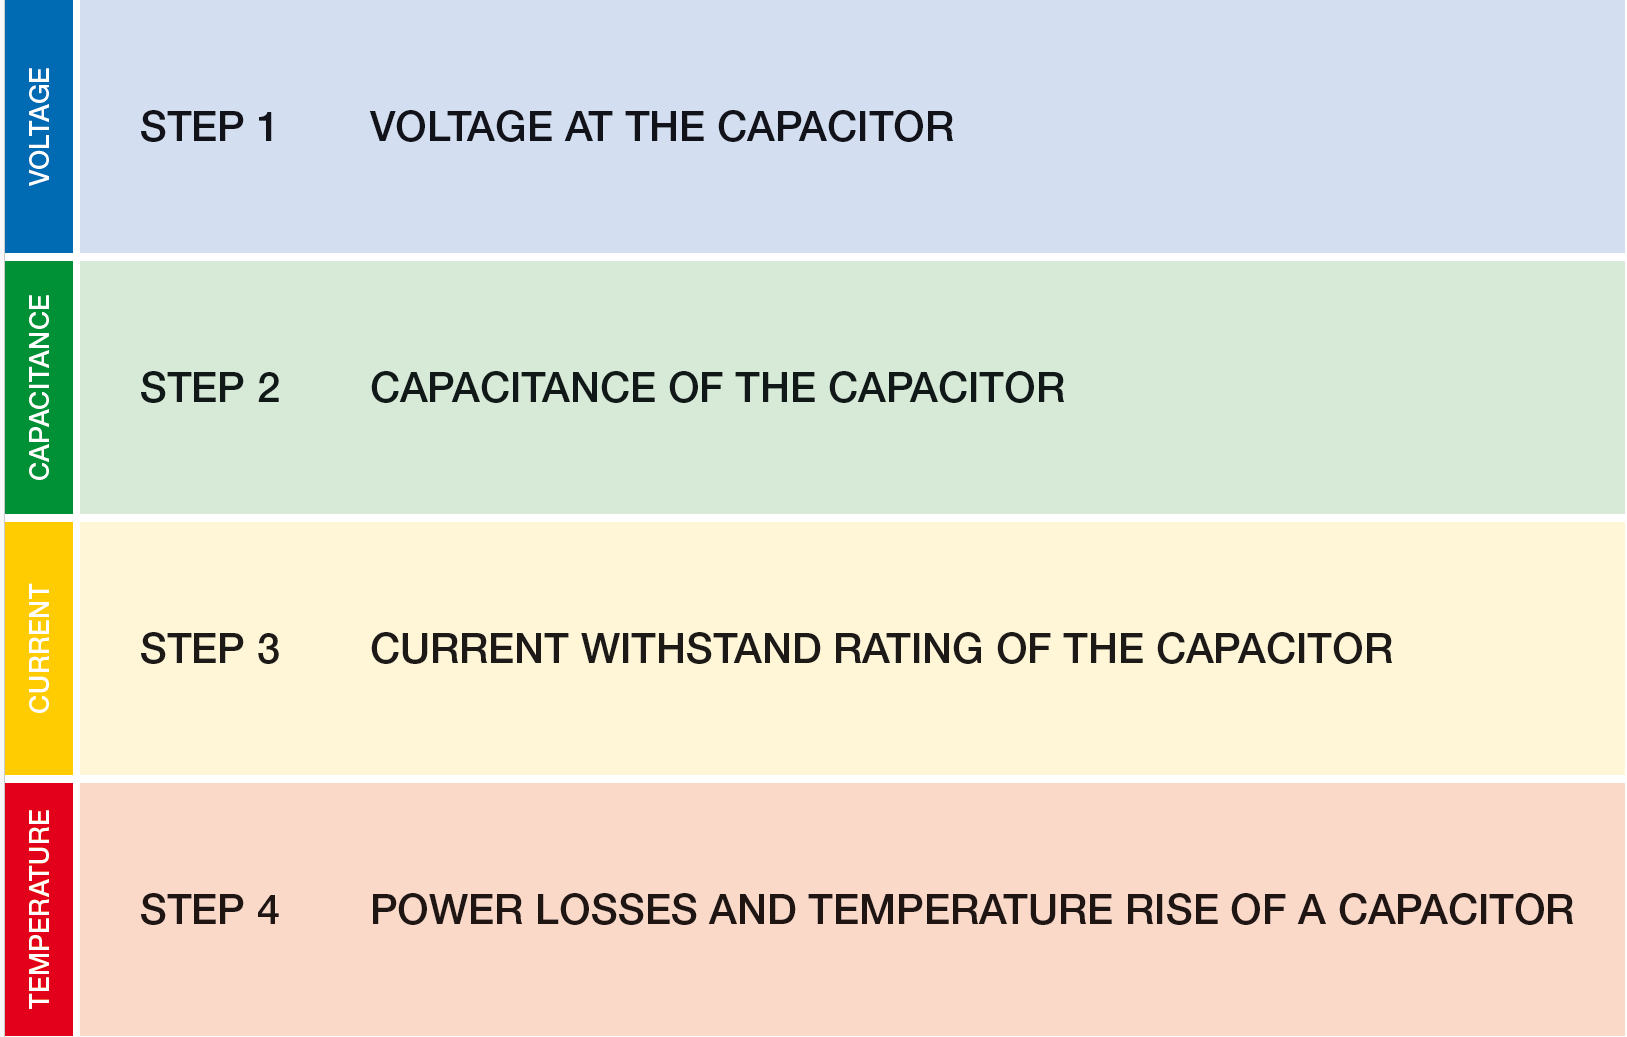
\includegraphics[width=\linewidth]{fig/lec08/selection_steps.png}
    \caption{Four-step selection procedure: voltage, capacitance, current withstand, and power-loss/temperature-rise verification. Adapted from FRAKO, \textit{Power Electronics Capacitors Selection Guide}}
\end{figure}
\end{column}
\end{columns}

\end{frame}


%%%%%%%%%%%%%%%%%%%%%%%%%%%%%%%%%%%%%%%%%%%%%%%%%%%%%%%%%%%%%
%% Selection workflow using circuitikz
%%%%%%%%%%%%%%%%%%%%%%%%%%%%%%%%%%%%%%%%%%%%%%%%%%%%%%%%%%%%%
\begin{frame}
\frametitle{Engineering Workflow for Capacitor Selection}

\begin{center}
\begin{circuitikz}[scale=0.73, transform shape]
    \tikzstyle{block} = [draw, rounded corners, align=center,
    minimum width=2.7cm, minimum height=0.75cm, font=\scriptsize]

    \node[block] (app) at (0,0) {Application\\function};
    \node[block] (volt) at (3.3,0) {Voltage rating\\and derating};
    \node[block] (cap) at (6.6,0) {Capacitance\\requirement};
    \node[block] (curr) at (9.9,0) {RMS and peak\\current rating};

    \node[block] (loss) at (9.9,-2.0) {Loss and\\temperature rise};
    \node[block] (imp) at (6.6,-2.0) {ESR, ESL and\\resonance};
    \node[block] (life) at (3.3,-2.0) {Lifetime and\\end-of-life};
    \node[block] (layout) at (0,-2.0) {Layout, cooling\\and mounting};

    \node[block, minimum width=3.2cm] (valid) at (4.95,-4.0) {Prototype, measurement\\and iteration};

    \draw[->, thick] (app) -- (volt);
    \draw[->, thick] (volt) -- (cap);
    \draw[->, thick] (cap) -- (curr);
    \draw[->, thick] (curr) -- (loss);
    \draw[->, thick] (loss) -- (imp);
    \draw[->, thick] (imp) -- (life);
    \draw[->, thick] (life) -- (layout);
    \draw[->, thick] (layout) -- (valid);

    \draw[->, thick, dashed] (valid.north) .. controls (4.95,-1.0) and (1.5,-1.0) .. (app.south);
\end{circuitikz}
\end{center}

\begin{block}{Message}
\small
Capacitor selection is iterative. Increasing capacitance may reduce voltage ripple, but it can increase volume, cost, inrush current and stored energy. Reducing ESR may improve heating, but layout ESL can still dominate high-frequency behaviour.
\end{block}

\end{frame}


%%%%%%%%%%%%%%%%%%%%%%%%%%%%%%%%%%%%%%%%%%%%%%%%%%%%%%%%%%%%%
%% Voltage rating and derating
%%%%%%%%%%%%%%%%%%%%%%%%%%%%%%%%%%%%%%%%%%%%%%%%%%%%%%%%%%%%%
\begin{frame}
\frametitle{Step 1: Voltage Rating and Derating}
The voltage rating must be selected from the worst-case voltage appearing at the capacitor terminals. The designer should consider:
\begin{itemize}
    \item nominal DC voltage and RMS AC voltage,
    \item peak repetitive voltage,
    \item switching overvoltage,
    \item surge voltage,
    \item regenerative or abnormal operating conditions,
    \item lifetime derating.
\end{itemize}
For DC operation,
\begin{align}
    V_{\mathrm{rated}} > V_{\mathrm{dc,max}}
\end{align}
For AC operation, the rated voltage must exceed the peak of the applied AC waveform:
\begin{align}
    V_{\mathrm{rated}} > V_{\mathrm{pk}}
\end{align}
In PWM filter applications, the capacitor peak voltage can be higher than the inverter DC-bus voltage due to switching and resonance effects.
\end{frame}


%%%%%%%%%%%%%%%%%%%%%%%%%%%%%%%%%%%%%%%%%%%%%%%%%%%%%%%%%%%%%
%% Capacitor voltage rating and capacitance selection
%%%%%%%%%%%%%%%%%%%%%%%%%%%%%%%%%%%%%%%%%%%%%%%%%%%%%%%%%%%%%
\begin{frame}
\frametitle{Example: Voltage Rating and Capacitance Selection}

\begin{columns}
\begin{column}{0.56\textwidth}
\textbf{Example:}
\begin{align}
    V_{\mathrm{pk,max}} = 420~\si{\volt}
    \quad \Rightarrow \quad
    V_N = 450~\si{\volt}
\end{align}
\begin{itemize}
    \item Choose the next higher catalogue voltage class.
    \item Include steady-state voltage, transients and safety margin.
    \item In PWM filter applications, the capacitor peak voltage can be higher than the inverter DC-bus voltage.
\end{itemize}
\end{column}

\begin{column}{0.40\textwidth}
\begin{block}{Selection Logic}
Once the voltage class is fixed, select the capacitance from the catalogue based on:
\begin{itemize}
    \item required capacitance,
    \item RMS current rating,
    \item peak current capability,
    \item thermal resistance,
    \item ESR and dimensions.
\end{itemize}
\end{block}

\begin{block}{Example Target}
\small
\[
V_N = 450~\si{\volt}, 
\qquad
C_{\mathrm{desired}} = 50~\si{\micro\farad}
\]
\end{block}
\end{column}
\end{columns}

\end{frame}


%%%%%%%%%%%%%%%%%%%%%%%%%%%%%%%%%%%%%%%%%%%%%%%%%%%%%%%%%%%%%
%% Catalogue-based capacitor selection
%%%%%%%%%%%%%%%%%%%%%%%%%%%%%%%%%%%%%%%%%%%%%%%%%%%%%%%%%%%%%
\begin{frame}
\frametitle{Catalogue-Based Capacitor Selection Example}
\small
For a three-phase AC filter capacitor with
\[
V_N = 450~\si{\volt},
\qquad
C_{\mathrm{desired}} = 50~\si{\micro\farad},
\]
the closest catalogue choice is selected from the 450~V capacitor family.

\begin{table}
\centering
\scriptsize
\renewcommand{\arraystretch}{1.15}
\begin{tabular}{p{0.17\textwidth}p{0.22\textwidth}c c c c c}
\hline
\textbf{Article No.} & \textbf{Type} & 
\textbf{$C$} & 
\textbf{$I_{\max}$} & 
\textbf{$\hat{i}$} & 
\textbf{$R_{\mathrm{th}}$} & 
\textbf{$R_s$} \\
 & & 
\textbf{in $\si{\micro\farad}$} & 
\textbf{in A} & 
\textbf{in kA} & 
\textbf{in K/W} & 
\textbf{in m$\Omega$} \\
\hline
31-13002 & LKT-F-040.0-3-450-BF & $3\times40$ & 28 & 1.4 & $\leq 3.5$ & 1.79 \\

\rowcolor{green!15}
31-13003 & LKT-F-050.0-3-450-BF & $3\times50$ & 28 & 1.7 & $\leq 3.5$ & 1.66 \\

31-13004 & LKT-F-075.0-3-450-BF & $3\times75$ & 28 & 2.6 & $\leq 3.5$ & 1.49 \\
\hline
\end{tabular}
\end{table}

\vspace{0.1cm}

\begin{block}{Selected Component}
\small
The suitable choice is:
\[
\boxed{\text{LKT-F-050.0-3-450-BF}}
\]
because it matches the required voltage class and capacitance:
\[
V_N = 450~\si{\volt},
\qquad
C = 3\times50~\si{\micro\farad}.
\]
\end{block}
\end{frame}


%%%%%%%%%%%%%%%%%%%%%%%%%%%%%%%%%%%%%%%%%%%%%%%%%%%%%%%%%%%%%
%% Capacitance from ripple
%%%%%%%%%%%%%%%%%%%%%%%%%%%%%%%%%%%%%%%%%%%%%%%%%%%%%%%%%%%%%
\begin{frame}
\frametitle{Step 2: Capacitance from Ripple-Voltage Requirement}

\begin{columns}
\begin{column}{0.56\textwidth}
One common sizing criterion is the maximum allowable voltage ripple. If the capacitor current is approximately known, the voltage ripple can be estimated from the capacitor impedance:
\begin{align}
    \hat{U}_{r}
    =
    \hat{I}_{r}
    \left|
    \frac{1}{j2\pi f C}
    +
    ESR
    \right|
\end{align}
Neglecting ESL, the ripple magnitude becomes
\begin{align}
    U_r
    =
    I_r
    \sqrt{
    \frac{1}{4\pi^2 f^2 C^2}
    +
    ESR^2
    }
\end{align}
Therefore, the capacitance must be large enough so that
\begin{align}
    U_r < U_{r,\max}
\end{align}
\end{column}

\begin{column}{0.40\textwidth}
\begin{block}{Design Interpretation}
At low frequency, the capacitive term dominates:
\[
\frac{1}{2\pi f C}
\]
At higher frequency, ESR and ESL can dominate. Therefore, simply increasing \(C\) may not reduce ripple if ESR or ESL is already limiting the impedance.
\end{block}

\begin{block}{Important}
\small
Use the effective capacitance at operating voltage, temperature and frequency, especially for MLCCs.
\end{block}
\end{column}
\end{columns}
\end{frame}


%%%%%%%%%%%%%%%%%%%%%%%%%%%%%%%%%%%%%%%%%%%%%%%%%%%%%%%%%%%%%
%% Capacitance from hold-up energy
%%%%%%%%%%%%%%%%%%%%%%%%%%%%%%%%%%%%%%%%%%%%%%%%%%%%%%%%%%%%%
\begin{frame}
\frametitle{Step 2: Capacitance from Hold-Up Energy}
\begin{columns}
\begin{column}{0.56\textwidth}
In DC-link and hold-up applications, the capacitor is sized from the energy required during a temporary input interruption or power mismatch. The stored energy is
\begin{align}
    E_C = \frac{1}{2}CV^2
\end{align}
If the capacitor supplies power \(P\) for a hold-up time \(t_h\), then
\begin{align}
    P t_h
    =
    \frac{1}{2}C
    \left(
    V_{\max}^2 - V_{\min}^2
    \right)
\end{align}
Thus,
\begin{align}
    C
    =
    \frac{2Pt_h}
    {V_{\max}^2 - V_{\min}^2}
\end{align}
This method is common in DC-link design, UPS systems, auxiliary supplies and ride-through energy buffers.
\end{column}

\begin{column}{0.40\textwidth}
\begin{block}{Power Electronics Interpretation}
\small
Capacitance requirement can come from different constraints:
\begin{itemize}
    \item ripple voltage,
    \item hold-up energy,
    \item transient load step,
    \item stability,
    \item impedance target.
\end{itemize}
The largest resulting capacitance is usually the starting design value.
\end{block}
\end{column}
\end{columns}

\end{frame}


%%%%%%%%%%%%%%%%%%%%%%%%%%%%%%%%%%%%%%%%%%%%%%%%%%%%%%%%%%%%%
%% DC-link sizing criteria
%%%%%%%%%%%%%%%%%%%%%%%%%%%%%%%%%%%%%%%%%%%%%%%%%%%%%%%%%%%%%
\begin{frame}
\frametitle{DC-Link Capacitor Sizing Criteria}
\begin{columns}
\begin{column}{0.56\textwidth}
DC-link capacitor sizing is application-specific. A single equation is rarely sufficient. Important sizing criteria include:
\begin{itemize}
    \item steady-state DC-link voltage ripple,
    \item transient and abnormal-operation voltage ripple,
    \item energy-storage or hold-up requirement,
    \item stability of cascaded converter stages,
    \item RMS ripple-current capability,
    \item temperature range and capacitance stability,
    \item frequency characteristics,
    \item lifetime and end-of-life tolerance.
\end{itemize}
\end{column}

\begin{column}{0.40\textwidth}
    \vspace{-1cm}
    \begin{figure}
        \centering
        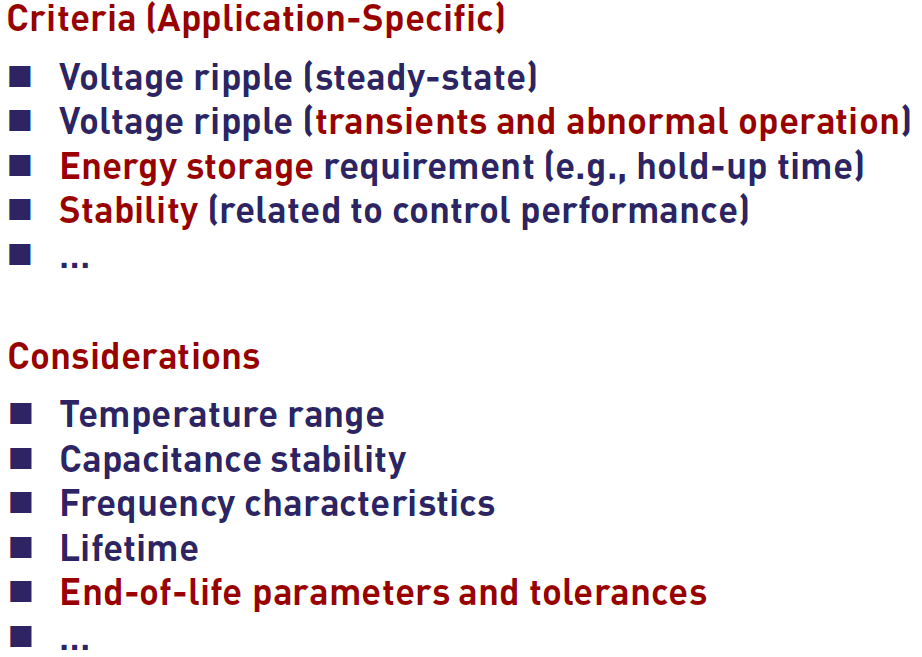
\includegraphics[width=\linewidth]{fig/lec08/DC_link_sizing_criteria.png}
        \caption{DC-link capacitor sizing criteria and practical considerations, Adapted from Huai Wang, \textit{Capacitors in Power Electronics Applications -- Reliability and Circuit Design}, IECON 2016 tutorial.}
    \end{figure}
\end{column}
\end{columns}
For high-reliability systems, the DC-link capacitor should be designed from the mission profile, not only from a single rated operating point.
\end{frame}


%%%%%%%%%%%%%%%%%%%%%%%%%%%%%%%%%%%%%%%%%%%%%%%%%%%%%%%%%%%%%
%% Ripple current and peak current
%%%%%%%%%%%%%%%%%%%%%%%%%%%%%%%%%%%%%%%%%%%%%%%%%%%%%%%%%%%%%
\begin{frame}
\frametitle{Step 3: RMS and Peak Current Rating}
The capacitor must withstand both RMS ripple current and peak current. The peak current caused by a voltage transition is
\begin{align}
    I_{\mathrm{pk}}
    =
    C\frac{dv}{dt}
\end{align}
The RMS current determines heating:
\begin{align}
    P_{\mathrm{ohmic}}
    =
    I_{\mathrm{rms}}^2 R_s
\end{align}
For a non-sinusoidal capacitor current composed of harmonics,
\begin{align}
    I_{\mathrm{rms}}
    =
    \sqrt{
    I_1^2+I_2^2+I_3^2+\cdots+I_n^2
    }
\end{align}
This is important because power-converter capacitor current is usually pulsed or nonsinusoidal.
\end{frame}

%%%%%%%%%%%%%%%%%%%%%%%%%%%%%%%%%%%%%%%%%%%%%%%%%%%%%%%%%%%%%
%% Losses and temperature rise
%%%%%%%%%%%%%%%%%%%%%%%%%%%%%%%%%%%%%%%%%%%%%%%%%%%%%%%%%%%%%
\begin{frame}
\frametitle{Step 4: Losses and Temperature Rise}
\begin{columns}
\begin{column}{0.56\textwidth}
After the voltage, capacitance and current ratings are selected, the thermal operating point must be checked. The total capacitor loss is
\begin{align}
    P_{\mathrm{loss}}
    =
    P_{\mathrm{ohmic}}
    +
    P_{\mathrm{dielectric}}
\end{align}
where
\begin{align}
    P_{\mathrm{ohmic}}
    =
    I_{\mathrm{rms}}^2R_s
\end{align}
and, for sinusoidal AC operation,
\begin{align}
    P_{\mathrm{dielectric}}
    =
    V_{\mathrm{pp}}^2\pi f_0 C \tan\delta_0
\end{align}
The temperature rise is
\begin{align}
    \Delta T
    =
    R_{\mathrm{th}}P_{\mathrm{loss}}
\end{align}
The design is acceptable only if the hot-spot temperature remains below the specified limit.
\end{column}
\begin{column}{0.40\textwidth}
    \vspace{-1cm}
\begin{figure}
    \centering
    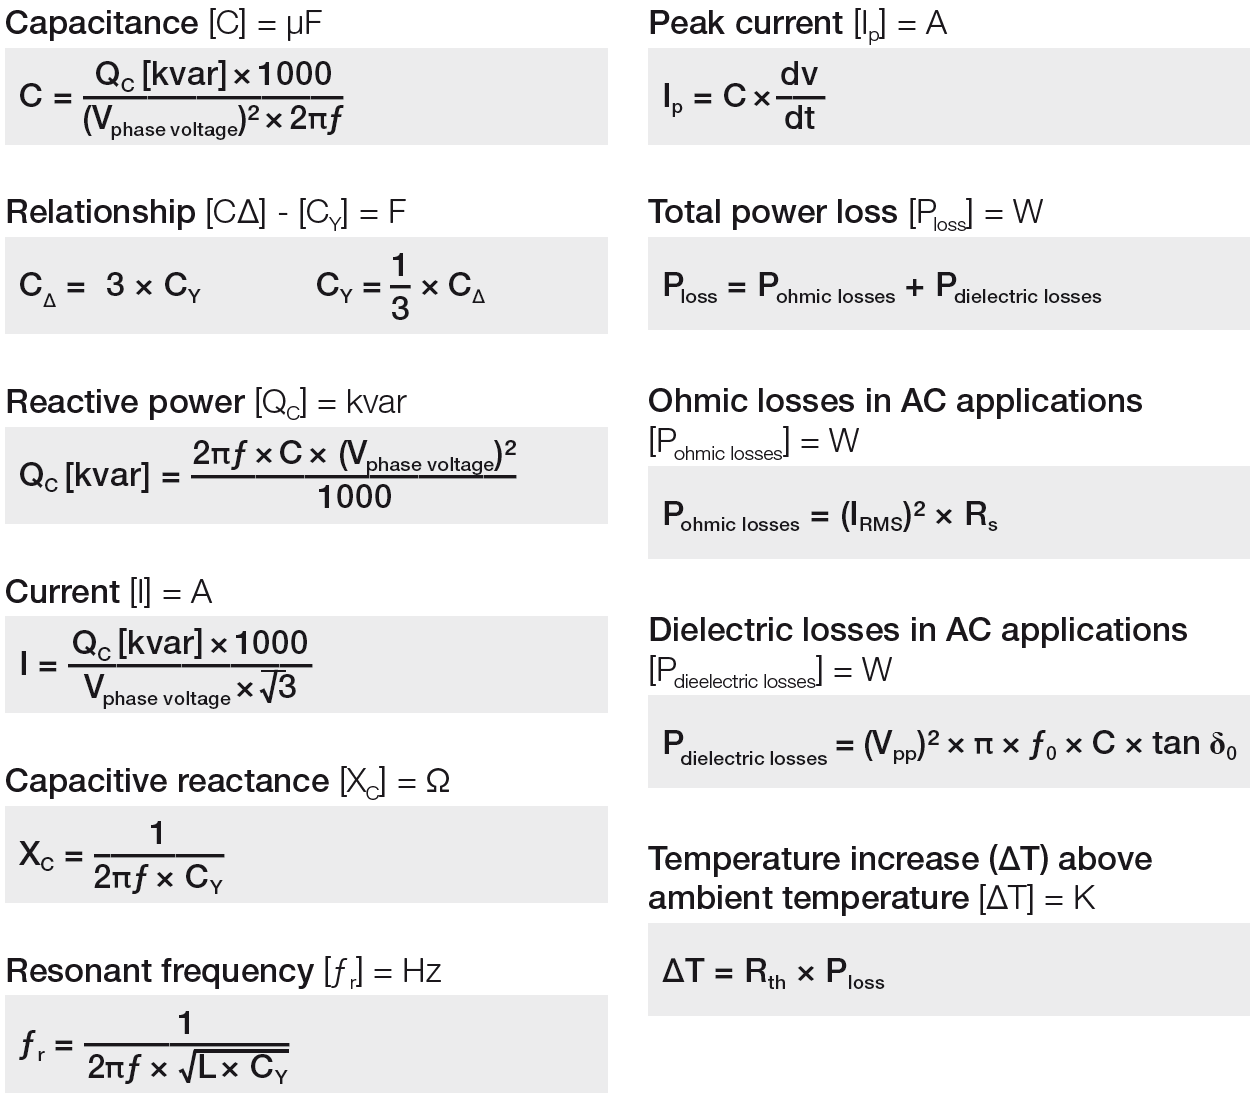
\includegraphics[width=\linewidth]{fig/lec08/losses_temperature_formulas.png}
    \caption{Useful power-electronics capacitor formulas for peak current, ohmic loss, dielectric loss and temperature rise. Adapted from FRAKO, \textit{Power Electronics Capacitors Selection Guide}}
\end{figure}
\end{column}
\end{columns}
\end{frame}


%%%%%%%%%%%%%%%%%%%%%%%%%%%%%%%%%%%%%%%%%%%%%%%%%%%%%%%%%%%%%
%% Series capacitor connection
%%%%%%%%%%%%%%%%%%%%%%%%%%%%%%%%%%%%%%%%%%%%%%%%%%%%%%%%%%%%%
\begin{frame}
\frametitle{Series Connection of Capacitors}

\begin{columns}
\begin{column}{0.56\textwidth}
Capacitors are connected in series when the required voltage rating exceeds the rating of one capacitor. For two capacitors in series,
\begin{align}
    C_{\mathrm{eq}}
    =
    \frac{C_1C_2}{C_1+C_2}
\end{align}
For identical capacitors, $C_{\mathrm{eq}}=\frac{C}{n}$, where \(n\) is the number of series-connected capacitors. The voltage sharing is affected by:
\begin{itemize}
    \item capacitance tolerance,
    \item leakage-current mismatch,
    \item insulation resistance mismatch,
    \item temperature variation and ageing.
\end{itemize}
Voltage-balancing resistors or active balancing circuits are therefore often required.
\end{column}

\begin{column}{0.40\textwidth}
    \vspace{-0.75cm}
\begin{figure}
    \centering
    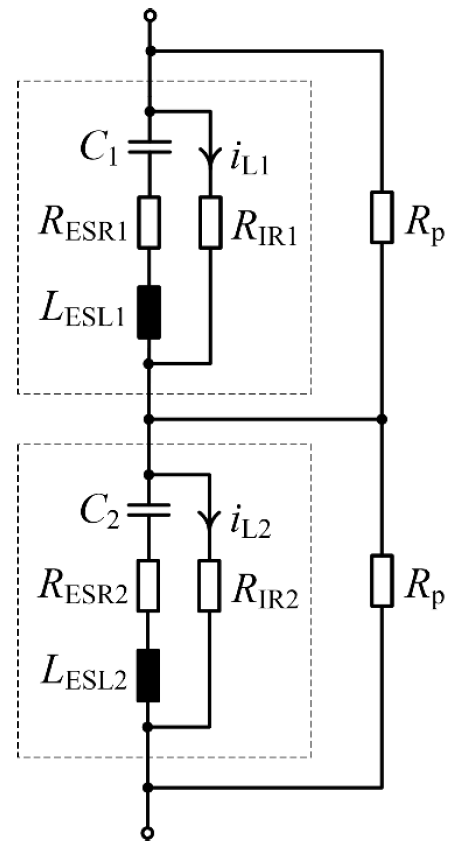
\includegraphics[width=0.4\linewidth]{fig/lec08/series_capacitor_balancing.png}
    \caption{Voltage balancing of series-connected capacitors with insulation resistance, leakage current and balancing resistance. Adapted from Huai Wang, \textit{Capacitors in Power Electronics Applications -- Reliability and Circuit Design}, IECON 2016 tutorial}
\end{figure}
\end{column}
\end{columns}
\end{frame}


%%%%%%%%%%%%%%%%%%%%%%%%%%%%%%%%%%%%%%%%%%%%%%%%%%%%%%%%%%%%%
%% Parallel capacitor connection
%%%%%%%%%%%%%%%%%%%%%%%%%%%%%%%%%%%%%%%%%%%%%%%%%%%%%%%%%%%%%
\begin{frame}
\frametitle{Parallel Connection of Capacitors}

\begin{columns}
\begin{column}{0.56\textwidth}
Capacitors are connected in parallel to increase capacitance, ripple-current capability, and reduce equivalent ESR. For capacitors connected in parallel,
\begin{align}
    C_{\mathrm{eq}}
    =
    C_1+C_2+C_3+\cdots
\end{align}
The equivalent ESR ideally becomes
\begin{align}
    ESR_{\mathrm{eq}}
    \approx
    \frac{ESR}{n}
\end{align}
for \(n\) identical capacitors. However, current sharing is not automatically equal. It depends on:
\begin{itemize}
    \item ESR and ESL mismatch,
    \item layout symmetry,
    \item terminal impedance,
    \item frequency.
\end{itemize}
\end{column}

\begin{column}{0.40\textwidth}
\begin{center}
\begin{circuitikz}[scale=0.82, transform shape]
    \draw (0,0) -- (4.2,0);
    \draw (0,-2.2) -- (4.2,-2.2);

    \draw (0.7,0) to[C,l=$C_1$] (0.7,-2.2);
    \draw (2.1,0) to[C,l=$C_2$] (2.1,-2.2);
    \draw (3.5,0) to[C,l=$C_3$] (3.5,-2.2);

    \draw[->, thick] (-0.5,-1.1) -- (0.2,-1.1);
    \node at (-0.85,-1.1) {$i_C$};

    \node at (2.1,-2.8) {\small parallel bank for higher current capability};
\end{circuitikz}
\end{center}
\begin{block}{Design Message}
\small
Parallel connection is effective only when the physical layout provides comparable impedance paths to all capacitors.
\end{block}
\end{column}
\end{columns}
A poor layout can cause one capacitor to carry excessive ripple current.
\end{frame}


%%%%%%%%%%%%%%%%%%%%%%%%%%%%%%%%%%%%%%%%%%%%%%%%%%%%%%%%%%%%%
%% Hybrid DC-link bank
%%%%%%%%%%%%%%%%%%%%%%%%%%%%%%%%%%%%%%%%%%%%%%%%%%%%%%%%%%%%%
\begin{frame}
\frametitle{Hybrid DC-Link Capacitor Bank}
\begin{columns}
\begin{column}{0.56\textwidth}
A hybrid DC-link bank combines capacitor technologies to exploit their complementary strengths. Typical arrangement:
\begin{itemize}
    \item electrolytic capacitors = large energy storage,
    \item film capacitors carry high ripple current and reduce mid-frequency impedance,
    \item ceramic or power ceramic capacitors suppress high-frequency switching transients.
\end{itemize}
This strategy improves:
\begin{itemize}
    \item ripple-current sharing and voltage ripple reduction,
    \item high-frequency decoupling and thermal distribution,
    \item lifetime of the electrolytic bank.
\end{itemize}
\end{column}

\begin{column}{0.40\textwidth}
    \vspace{-0.75cm}
\begin{figure}
    \centering
    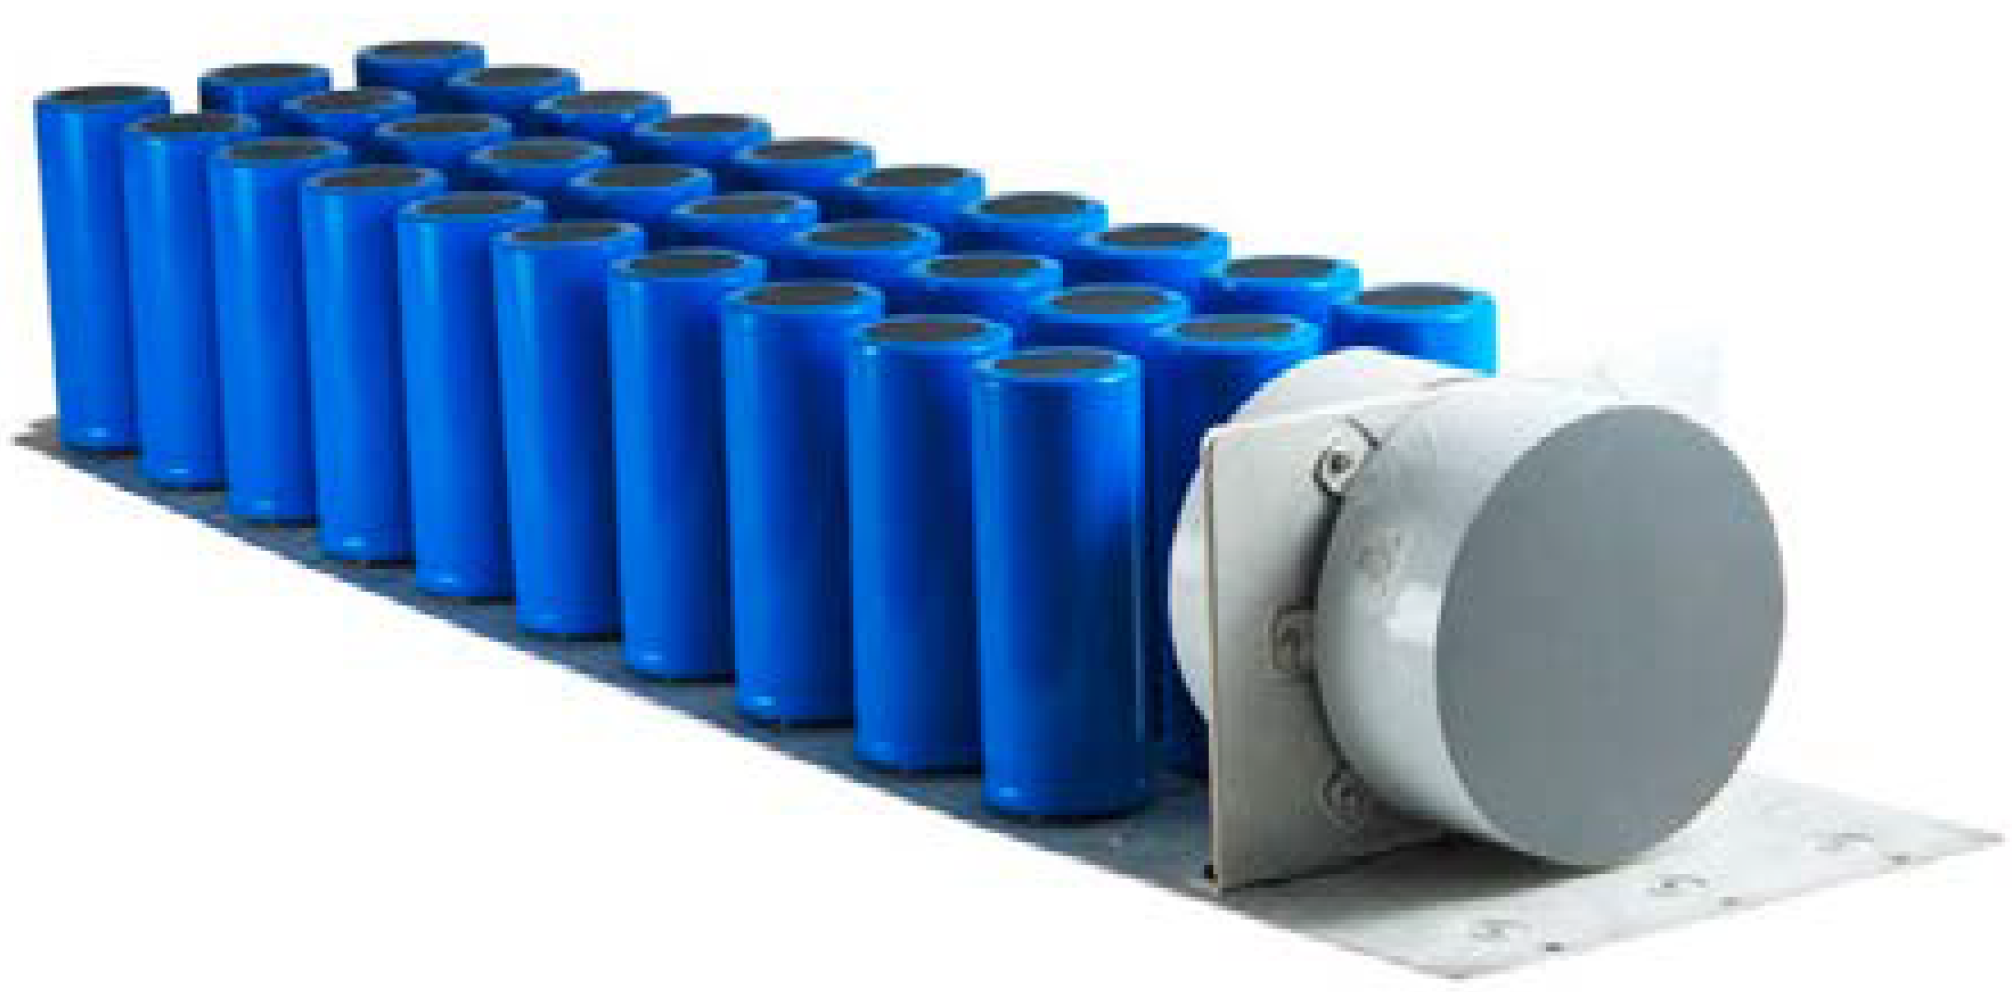
\includegraphics[width=\linewidth]{fig/lec08/hybrid_DC_link_bank.png}
    \caption{Hybrid DC-link capacitor bank showing ripple-current harmonic reduction by adding a film capacitor in parallel with an electrolytic bank. Adapted from Huai Wang, \textit{Capacitors in Power Electronics Applications -- Reliability and Circuit Design}, IECON 2016 tutorial}
\end{figure}
\end{column}
\end{columns}
The bank must still be checked for anti-resonance and layout-induced current imbalance.
\end{frame}


%%%%%%%%%%%%%%%%%%%%%%%%%%%%%%%%%%%%%%%%%%%%%%%%%%%%%%%%%%%%%
%% Low inductance DC link layout
%%%%%%%%%%%%%%%%%%%%%%%%%%%%%%%%%%%%%%%%%%%%%%%%%%%%%%%%%%%%%
\begin{frame}
\frametitle{Low-Inductance DC-Link Layout}
In fast-switching converters, the physical capacitor-bank layout can be as important as the capacitor datasheet. The DC-link loop inductance causes switching overvoltage:
\begin{align}
    v_{\sigma}
    =
    L_{\sigma}\frac{di}{dt}
\end{align}
Low-inductance design requires:
\begin{itemize}
    \item short current paths,
    \item laminated positive and negative busbars,
    \item magnetic-field cancellation,
    \item symmetric capacitor placement,
    \item local high-frequency capacitors near devices,
    \item minimized commutation-loop area.
\end{itemize}
For SiC and GaN converters, a low-ESL capacitor is insufficient if the busbar or PCB layout has large loop inductance.

\end{frame}

\begin{frame}
\frametitle{Low-Inductance DC-Link Layout}
\begin{figure}
    \centering
    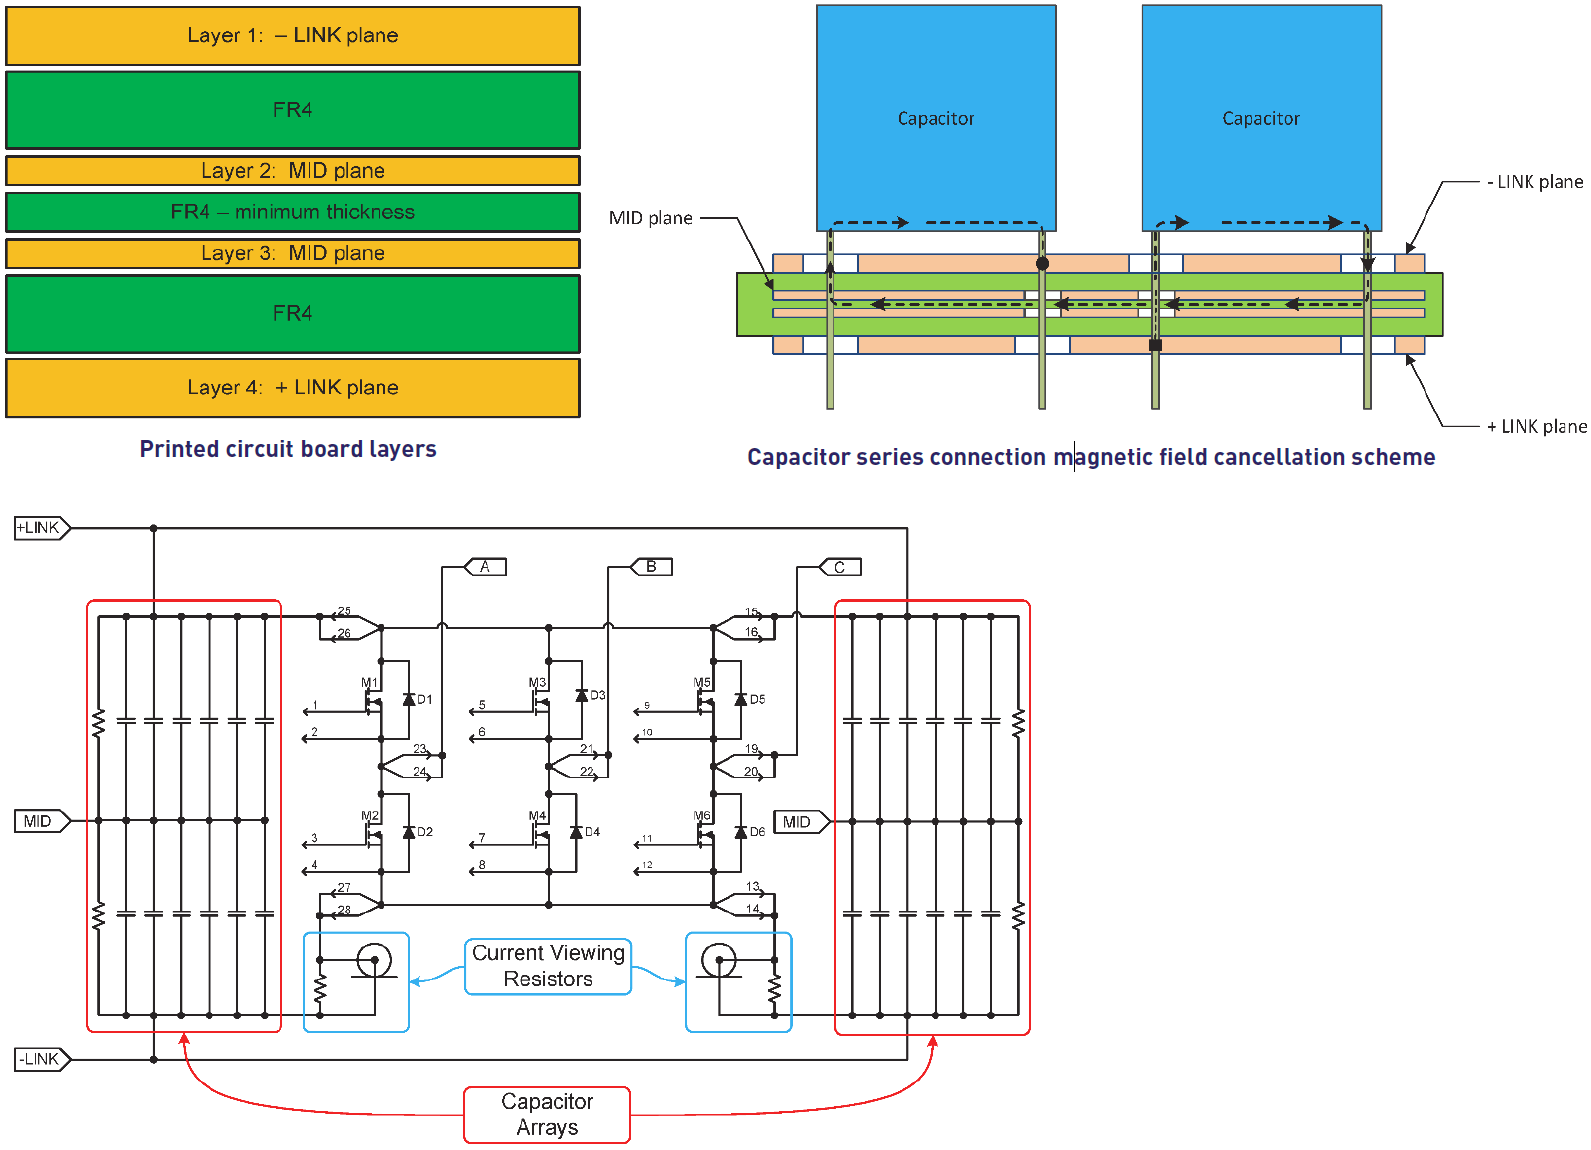
\includegraphics[width=0.5\linewidth]{fig/lec08/low_inductance_bank.png}
    \caption{Low-inductance capacitor-bank design using magnetic-field cancellation and PCB/busbar layout concepts. Adapted from Huai Wang, \textit{Capacitors in Power Electronics Applications -- Reliability and Circuit Design}, IECON 2016 tutorial}
\end{figure}
\end{frame}

%%%%%%%%%%%%%%%%%%%%%%%%%%%%%%%%%%%%%%%%%%%%%%%%%%%%%%%%%%%%%
%% Selection verification checklist
%%%%%%%%%%%%%%%%%%%%%%%%%%%%%%%%%%%%%%%%%%%%%%%%%%%%%%%%%%%%%
\begin{frame}
\frametitle{Final Capacitor Selection Checklist}

\begin{itemize}
    \item \textbf{Voltage check:}
    \[
        V_{\mathrm{rated}} > V_{\mathrm{max,operating}} + V_{\mathrm{surge\ margin}}
    \]

    \item \textbf{Capacitance check:}
    \[
        C_{\mathrm{effective}} \geq C_{\mathrm{required}}
    \]
    using bias, temperature, tolerance and ageing corrections.

    \item \textbf{Ripple-current check:} $I_{\mathrm{C,rms}} < I_{\mathrm{rated,rms}}$.

    \item \textbf{Peak-current and \(dv/dt\) check:}
    \[
        I_{\mathrm{pk}} = C\frac{dv}{dt}
    \]

    \item \textbf{Thermal check:}
    \[
        T_{\mathrm{hotspot}} = T_{\mathrm{amb}} + R_{\mathrm{th}}P_{\mathrm{loss}}
    \]
    \item \textbf{Impedance check:}
    ESR, ESL, self-resonance, anti-resonance and layout parasitics must satisfy the required frequency-domain impedance.
    \item \textbf{Reliability check:}
    lifetime, end-of-life capacitance loss, ESR increase, leakage current and mission-profile stress must be acceptable.
\end{itemize}
\end{frame}


%%%%%%%%%%%%%%%%%%%%%%%%%%%%%%%%%%%%%%%%%%%%%%%%%%%%%%%%%%%%%
%% Losses, thermal design, reliability
%%%%%%%%%%%%%%%%%%%%%%%%%%%%%%%%%%%%%%%%%%%%%%%%%%%%%%%%%%%%%
\begin{frame}
\begin{center}
  \textbf{\Huge{Losses, Thermal Design, and Reliability}}\\[0.4cm]
  \textbf{\Large{From Electrical Stress to Lifetime and Condition Monitoring}}
\end{center}
\end{frame}


%%%%%%%%%%%%%%%%%%%%%%%%%%%%%%%%%%%%%%%%%%%%%%%%%%%%%%%%%%%%%
%% Loss mechanisms in capacitors
%%%%%%%%%%%%%%%%%%%%%%%%%%%%%%%%%%%%%%%%%%%%%%%%%%%%%%%%%%%%%
\begin{frame}
\frametitle{Loss Mechanisms in Capacitors}

\begin{columns}
\begin{column}{0.56\textwidth}
Real capacitors dissipate power due to ripple current, AC voltage, leakage, and switching transients. Main loss mechanisms:
\begin{itemize}
    \item \textbf{Ohmic loss:} caused by ESR under RMS ripple current.
    \item \textbf{Dielectric loss:} caused by polarization loss in the dielectric.
    \item \textbf{Leakage loss:} caused by finite insulation resistance.
    \item \textbf{Terminal and contact loss:} caused by current flowing through tabs, terminals, busbars, and solder joints.
    \item \textbf{Layout-related loss:} caused by high-frequency current crowding and parasitic inductance.
\end{itemize}
\end{column}

\begin{column}{0.44\textwidth}
\begin{center}
\begin{circuitikz}[scale=0.78, transform shape]
    \tikzstyle{block} = [draw, rounded corners, align=center,
    minimum width=2.4cm, minimum height=0.62cm, font=\scriptsize]

    \node[block, minimum width=3.0cm] (total) at (0,0) {Total capacitor\\loss};

    \node[block] (esr) at (-3.2,-1.5) {ESR\\loss};
    \node[block] (diel) at (0,-1.5) {Dielectric\\loss};
    \node[block] (leak) at (3.2,-1.5) {Leakage\\loss};

    \node[block] (ripple) at (-3.2,-3.0) {Ripple current\\$I_{\mathrm{rms}}$};
    \node[block] (tan) at (0,-3.0) {$\tan\delta$ and\\AC voltage};
    \node[block] (dc) at (3.2,-3.0) {DC voltage and\\insulation};

    \draw[->, thick] (total) -- (esr);
    \draw[->, thick] (total) -- (diel);
    \draw[->, thick] (total) -- (leak);

    \draw[->, thick] (esr) -- (ripple);
    \draw[->, thick] (diel) -- (tan);
    \draw[->, thick] (leak) -- (dc);
\end{circuitikz}
\end{center}

\end{column}
\end{columns}

\end{frame}


%%%%%%%%%%%%%%%%%%%%%%%%%%%%%%%%%%%%%%%%%%%%%%%%%%%%%%%%%%%%%
%% Loss mechanisms in capacitors
%%%%%%%%%%%%%%%%%%%%%%%%%%%%%%%%%%%%%%%%%%%%%%%%%%%%%%%%%%%%%
\begin{frame}
\frametitle{Loss Mechanisms in Capacitors}

\begin{columns}
\begin{column}{0.56\textwidth}
The first-order power loss is usually estimated as
\begin{align}
    P_{\mathrm{loss}}
    =
    I_{\mathrm{rms}}^2R_{\mathrm{ESR}}
    +
    P_{\mathrm{dielectric}}
    +
    P_{\mathrm{leak}}
\end{align}
\end{column}

\begin{column}{0.40\textwidth}
\begin{block}{Message}
\small
Capacitor loss is not only an efficiency issue. It directly determines hot-spot temperature, ageing speed, capacitance drift, ESR increase, and ultimately lifetime.
\end{block}
\end{column}
\end{columns}

\end{frame}

%%%%%%%%%%%%%%%%%%%%%%%%%%%%%%%%%%%%%%%%%%%%%%%%%%%%%%%%%%%%%
%% Thermal model
%%%%%%%%%%%%%%%%%%%%%%%%%%%%%%%%%%%%%%%%%%%%%%%%%%%%%%%%%%%%%
\begin{frame}
\frametitle{Thermal Model of a Capacitor}
\begin{columns}
\begin{column}{0.56\textwidth}
The losses generated inside the capacitor increase the internal hot-spot temperature. A first-order thermal model is
\begin{align}
    T_{\mathrm{hotspot}}
    =
    T_{\mathrm{amb}}
    +
    R_{\mathrm{th}}P_{\mathrm{loss}}
\end{align}
where
\begin{itemize}
    \item \(T_{\mathrm{hotspot}}\) is the internal hot-spot temperature,
    \item \(T_{\mathrm{amb}}\) is ambient temperature,
    \item \(R_{\mathrm{th}}\) is the thermal resistance from hot spot to ambient,
    \item \(P_{\mathrm{loss}}\) is total capacitor power loss.
\end{itemize}
The design must satisfy
\begin{align}
    T_{\mathrm{hotspot}} < T_{\mathrm{max}}
\end{align}
under worst-case ambient temperature, ripple current, cooling condition, and ageing state.
\end{column}

\begin{column}{0.40\textwidth}
\begin{center}
\begin{circuitikz}[scale=0.82, transform shape]
    \draw (0,0) to[I,l=$P_{\mathrm{loss}}$] (0,2.0);
    \draw (0,2.0) -- (1.6,2.0);
    \draw (1.6,2.0) to[R,l=$R_{\mathrm{th}}$] (1.6,0);
    \draw (1.6,0) -- (0,0);

    \node at (2.45,2.0) {$T_{\mathrm{hotspot}}$};
    \node at (2.25,0) {$T_{\mathrm{amb}}$};
    \node at (0.7,-0.45) {\small thermal equivalent circuit};
\end{circuitikz}
\end{center}

\begin{block}{Practical Note}
\small
For large-can electrolytic capacitors with significant ripple current, the internal core temperature can be noticeably higher than the case temperature. This must be considered during lifetime estimation.
\end{block}
\end{column}
\end{columns}

\end{frame}


%%%%%%%%%%%%%%%%%%%%%%%%%%%%%%%%%%%%%%%%%%%%%%%%%%%%%%%%%%%%%
%% Electrolytic capacitor lifetime
%%%%%%%%%%%%%%%%%%%%%%%%%%%%%%%%%%%%%%%%%%%%%%%%%%%%%%%%%%%%%
\begin{frame}
\frametitle{Aluminum Electrolytic Capacitor Lifetime}
\begin{columns}
\begin{column}{0.5\textwidth}
Aluminum electrolytic capacitors are often lifetime-critical because their electrolyte gradually evaporates or degrades during operation. The usual ageing effects are:
\begin{itemize}
    \item capacitance decreases,
    \item ESR increases,
    \item leakage current may change,
    \item internal temperature rises further due to higher ESR,
    \item open-circuit wear-out becomes likely.
\end{itemize}
\end{column}

\begin{column}{0.5\textwidth}
A commonly used lifetime expression is
\begin{align}
    L_{\mathrm{op}}
    =
    M_v L_b
    2^{(T_m-T_a)/10}
\end{align}
\begin{itemize}
    \item \(L_{\mathrm{op}}\) is expected operating life,
    \item \(L_b\) is base life,
    \item \(T_m\) is maximum permitted internal temperature,
    \item \(T_a\) is actual internal operating temperature,
    \item \(M_v\) accounts for voltage derating.
\end{itemize}
\end{column}
\end{columns}
\begin{block}{Rule of Thumb}
\small
For many aluminum electrolytic capacitors, operating life approximately doubles for every \(10^\circ\mathrm{C}\) reduction in internal temperature.
\end{block}
\end{frame}


%%%%%%%%%%%%%%%%%%%%%%%%%%%%%%%%%%%%%%%%%%%%%%%%%%%%%%%%%%%%%
%% Load life and end of life
%%%%%%%%%%%%%%%%%%%%%%%%%%%%%%%%%%%%%%%%%%%%%%%%%%%%%%%%%%%%%
\begin{frame}
\frametitle{Load Life Test and End-of-Life Criteria}
\begin{columns}
\begin{column}{0.56\textwidth}
Capacitor lifetime is usually specified under a rated load-life test condition. For aluminum electrolytic capacitors, the test commonly applies:
\begin{itemize}
    \item rated temperature,
    \item DC voltage,
    \item AC ripple current,
    \item specified test duration,
    \item post-test stabilization before measurement.
\end{itemize}
\end{column}

\begin{column}{0.40\textwidth}
\begin{block}{Design Message}
\small
The capacitor that satisfies capacitance and voltage on day one may still be unacceptable if its end-of-life capacitance, ESR, or leakage current violates converter requirements.
\end{block}
\end{column}
\end{columns}

\end{frame}


%%%%%%%%%%%%%%%%%%%%%%%%%%%%%%%%%%%%%%%%%%%%%%%%%%%%%%%%%%%%%
%% Load life and end of life
%%%%%%%%%%%%%%%%%%%%%%%%%%%%%%%%%%%%%%%%%%%%%%%%%%%%%%%%%%%%%
\begin{frame}
\frametitle{Load Life Test and End-of-Life Criteria}
\begin{columns}
\begin{column}{0.56\textwidth}
Typical end-of-life indicators include:
\begin{itemize}
    \item capacitance below an allowed fraction of initial value,
    \item ESR above an allowed limit,
    \item leakage current above specification,
    \item mechanical damage,
    \item electrolyte leakage,
    \item open-circuit or short-circuit failure.
\end{itemize}
\end{column}

\begin{column}{0.40\textwidth}
\begin{block}{Design Message}
\small
The capacitor that satisfies capacitance and voltage on day one may still be unacceptable if its end-of-life capacitance, ESR, or leakage current violates converter requirements.
\end{block}
\end{column}
\end{columns}
In converter design, lifetime should be evaluated at the actual hot-spot temperature and ripple-current condition, not only at datasheet nominal conditions.
\end{frame}

%%%%%%%%%%%%%%%%%%%%%%%%%%%%%%%%%%%%%%%%%%%%%%%%%%%%%%%%%%%%%
%% Load-life and ripple-life test
%%%%%%%%%%%%%%%%%%%%%%%%%%%%%%%%%%%%%%%%%%%%%%%%%%%%%%%%%%%%%
\begin{frame}
\frametitle{Load-Life and Ripple-Life Test of Capacitors}

\begin{columns}
\begin{column}{0.52\textwidth}
\textbf{Load-life test}
\begin{itemize}
    \item Capacitors are placed in a circulating-air oven at the upper rated temperature: $85^\circ\mathrm{C},\;105^\circ\mathrm{C},\;125^\circ\mathrm{C}$.
    \item A DC voltage and AC ripple voltage are applied simultaneously.
    \item The AC voltage is adjusted so that the rated ripple current flows.
    \item The DC voltage is adjusted so that the capacitor peak voltage equals the rated voltage.
    \item After the rated test duration, capacitors are stabilized at \(25^\circ\mathrm{C}\) for at least 24 h before measurement.
\end{itemize}
\end{column}

\begin{column}{0.48\textwidth}
\textbf{EIA ripple-life test}
\begin{itemize}
    \item Ripple current is usually applied at \(120~\si{\hertz}\).
    \item Test temperature is typically: $85 \pm 2^\circ\mathrm{C}$.
    \item Airflow is kept low to avoid excessive cooling.
    \item Samples are periodically measured during the test.
\end{itemize}
\begin{block}{End-of-Life Criteria}
\small
A capacitor reaches end of life if: 

$C < 80\%\,C_0 \quad \text{or}  \quad ESR > 200\%\,ESR_0  \quad \text{or}  \quad DCL > DCL_0$ or mechanical damage / electrolyte leakage is observed.
\end{block}
\end{column}
\end{columns}


\end{frame}

%%%%%%%%%%%%%%%%%%%%%%%%%%%%%%%%%%%%%%%%%%%%%%%%%%%%%%%%%%%%%
%% Failure modes aluminium electrolytic
%%%%%%%%%%%%%%%%%%%%%%%%%%%%%%%%%%%%%%%%%%%%%%%%%%%%%%%%%%%%%
\begin{frame}
\frametitle{Failure Modes of Aluminum Electrolytic Capacitors}
\begin{columns}
\begin{column}{0.56\textwidth}
Aluminum electrolytic capacitors can fail by early-life, random, or wear-out mechanisms.Important failure modes include:

\begin{itemize}
    \item \textbf{Open circuit:}
    \begin{itemize}
        \item electrolyte loss,
        \item terminal connection failure,
        \item internal pressure or venting.
    \end{itemize}

    \item \textbf{Short circuit:}
    \begin{itemize}
        \item oxide dielectric breakdown,
        \item severe overvoltage or thermal stress.
    \end{itemize}

    \item \textbf{Wear-out drift:}
    \begin{itemize}
        \item capacitance reduction,
        \item ESR and $\tan\delta$ increase
        \item leakage-current variation.
    \end{itemize}
\end{itemize}
\end{column}

\begin{column}{0.40\textwidth}
    \vspace{-0.5cm}
\begin{figure}
    \centering
    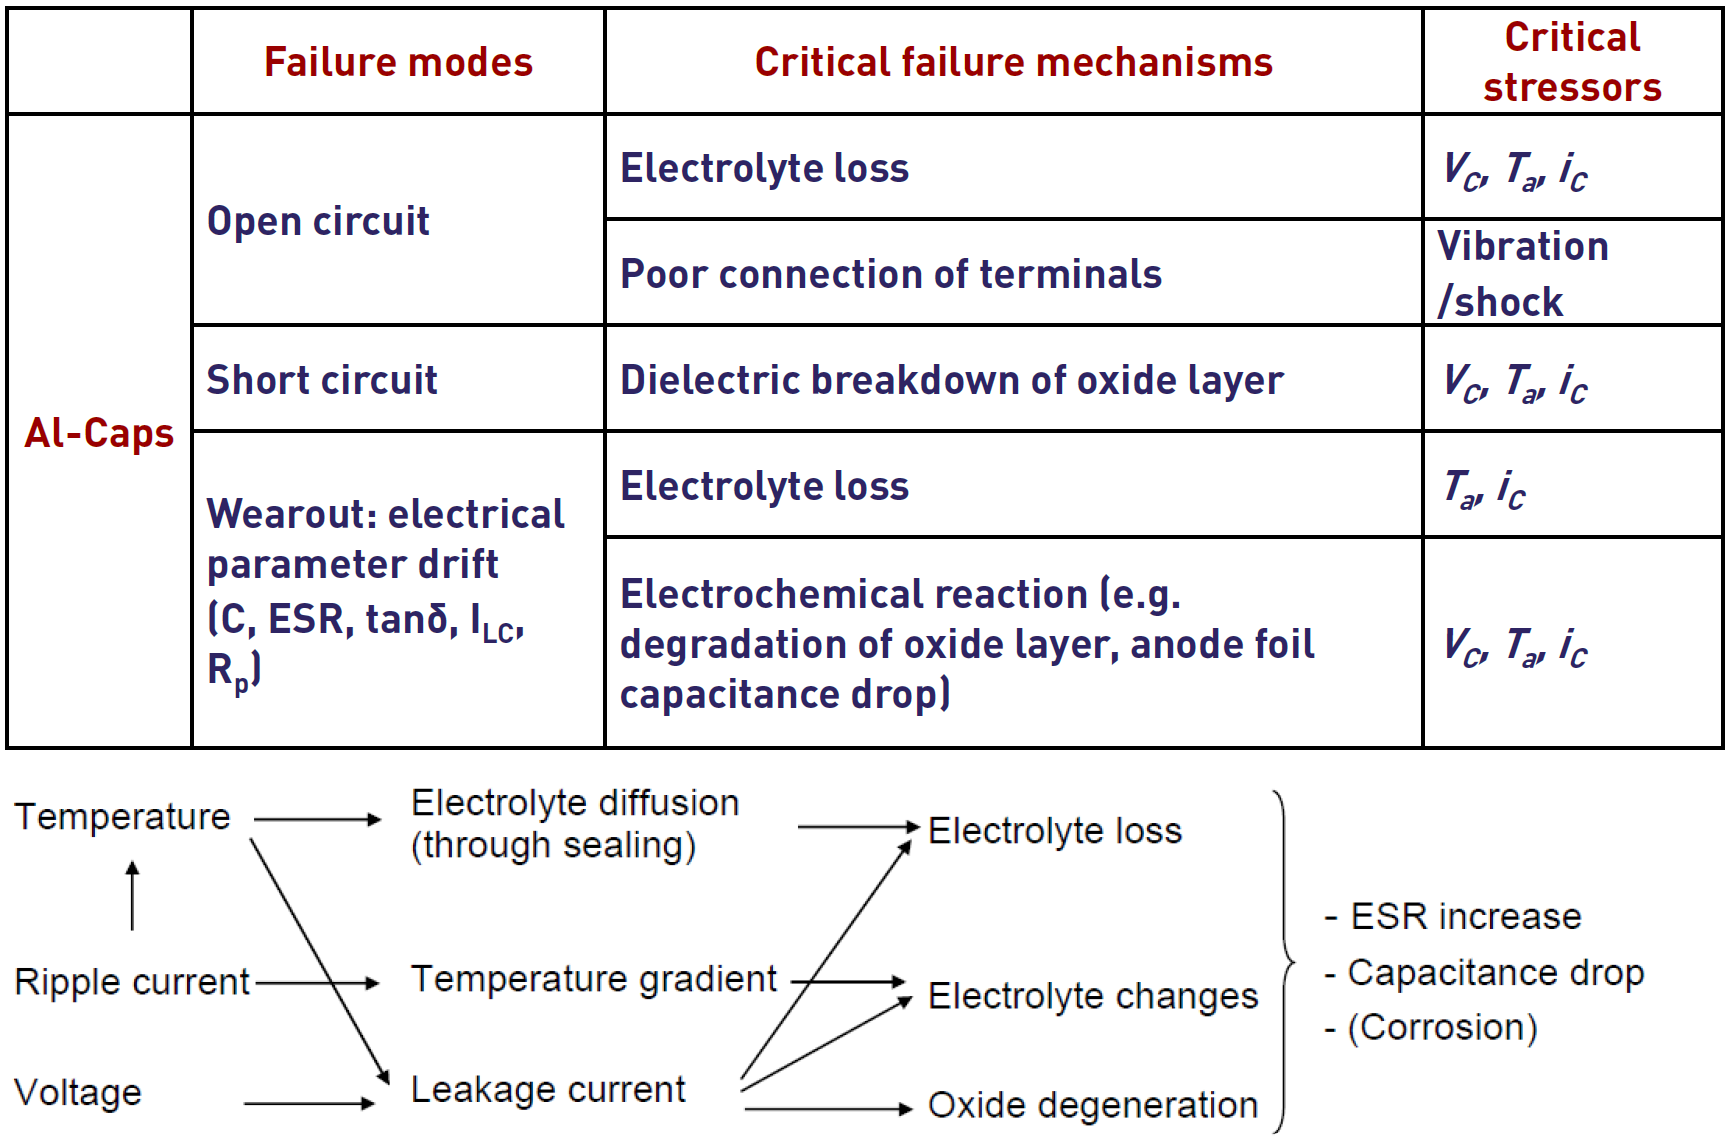
\includegraphics[width=\linewidth]{fig/lec08/AlCap_failure_modes.png}
    \caption{Failure modes, mechanisms, and critical stressors of aluminum electrolytic capacitors. Adapted from Huai Wang, \textit{Capacitors in Power Electronics Applications -- Reliability and Circuit Design}, IECON 2016 tutorial}
\end{figure}
\end{column}
\end{columns}
Critical stressors are voltage \(V_C\), ambient or hot-spot temperature \(T_a\), capacitor ripple current \(i_C\), and mechanical vibration or shock.
\end{frame}


%%%%%%%%%%%%%%%%%%%%%%%%%%%%%%%%%%%%%%%%%%%%%%%%%%%%%%%%%%%%%
%% Failure modes film capacitors
%%%%%%%%%%%%%%%%%%%%%%%%%%%%%%%%%%%%%%%%%%%%%%%%%%%%%%%%%%%%%
\begin{frame}
\frametitle{Failure Modes of Metallized Film Capacitors}
\begin{columns}
\begin{column}{0.56\textwidth}
Metallized polypropylene film capacitors are used in DC links, AC filters, and snubbers for low loss and self-healing. Main failure mechanisms are:
\begin{itemize}
    \item metallization corrosion due to humidity,
    \item capacitance loss from reduced active area,
    \item self-healing events under overvoltage or overcurrent,
    \item dielectric breakdown under high voltage or \(dv/dt\),
    \item connection instability from thermal and mechanical stress.
\end{itemize}
End-of-life usually shows gradual capacitance loss rather than sudden short circuit. Severe overvoltage, partial discharge, or thermal overload can still cause destructive failure.
\end{column}

\begin{column}{0.40\textwidth}
\begin{figure}
    \centering
    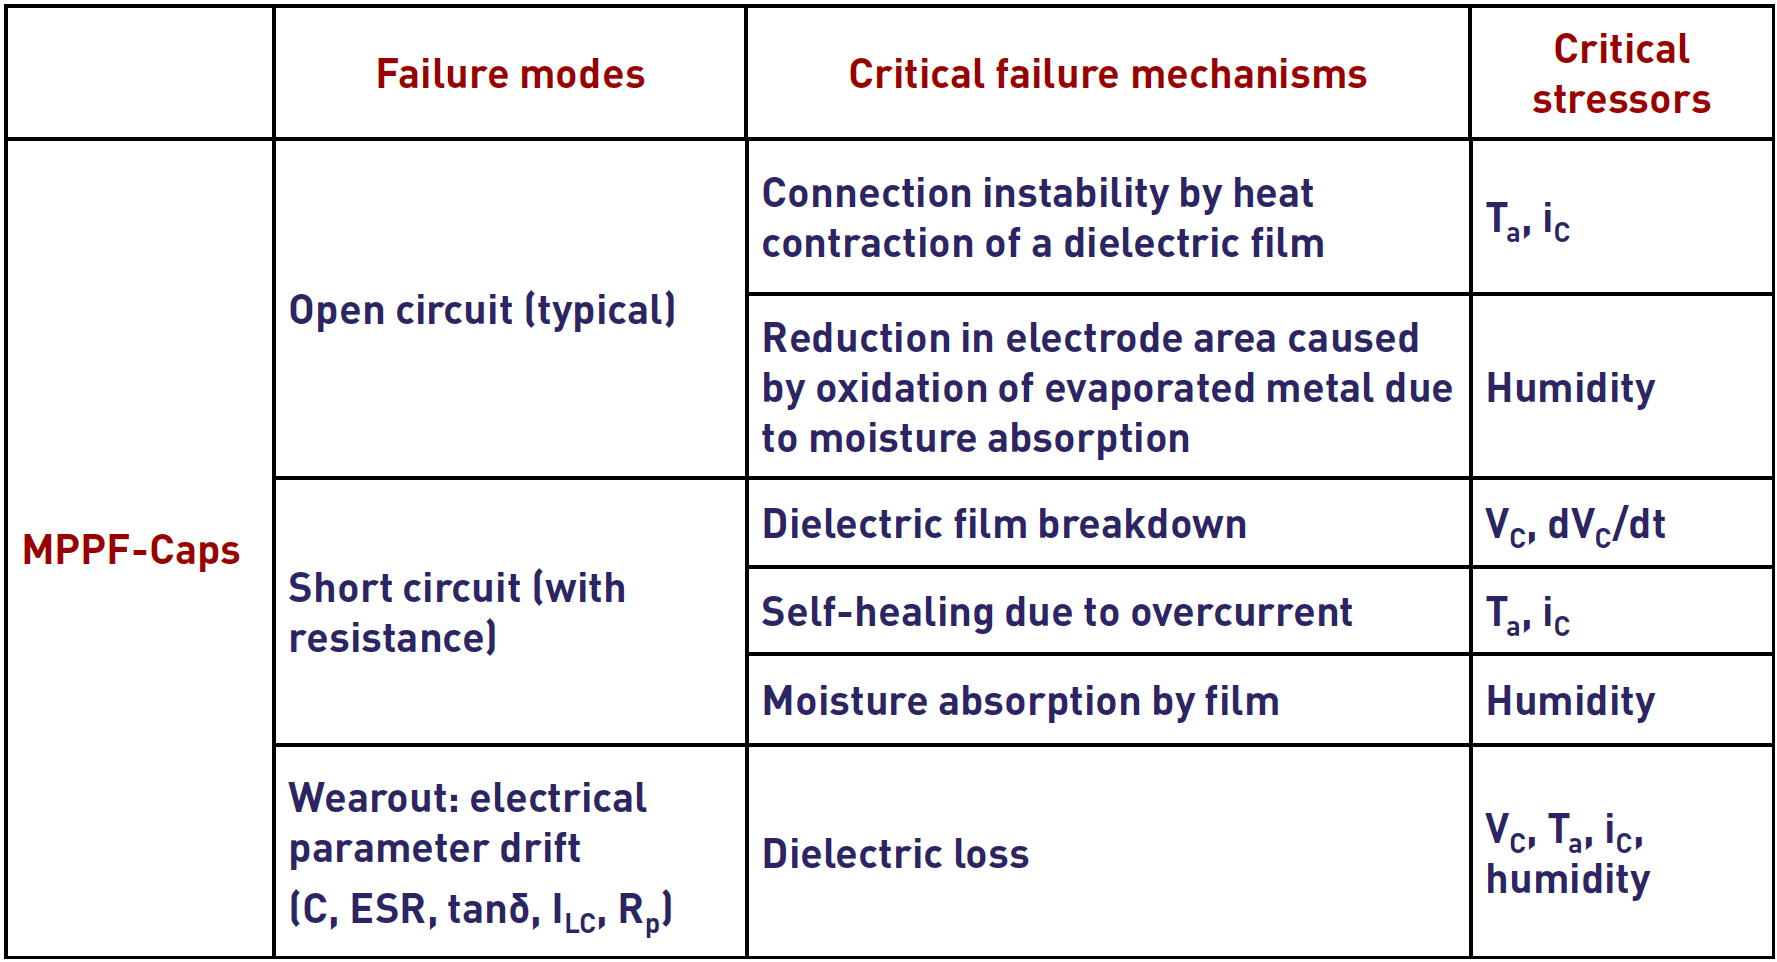
\includegraphics[width=\linewidth]{fig/lec08/MPPF_failure_modes.png}
    \caption{Failure modes, mechanisms, and critical stressors of metallized polypropylene film capacitors. Adapted from Huai Wang, \textit{Capacitors in Power Electronics Applications -- Reliability and Circuit Design}, IECON 2016 tutorial}
\end{figure}
\end{column}
\end{columns}

\end{frame}


%%%%%%%%%%%%%%%%%%%%%%%%%%%%%%%%%%%%%%%%%%%%%%%%%%%%%%%%%%%%%
%% Failure modes MLCC
%%%%%%%%%%%%%%%%%%%%%%%%%%%%%%%%%%%%%%%%%%%%%%%%%%%%%%%%%%%%%
\begin{frame}
\frametitle{Failure Modes of Multilayer Ceramic Capacitors}
\begin{columns}
\begin{column}{0.56\textwidth}
MLCCs offer excellent high-frequency performance, but fail differently from electrolytic and film capacitors. Key stress mechanisms include:

\begin{itemize}
    \item dielectric breakdown under voltage, temperature, and current stress,
    \item flex cracking from PCB bending,
    \item thermal shock cracking,
    \item mechanical damage during assembly,
    \item insulation degradation,
    \item micro-crack growth in the ceramic body.
\end{itemize}
A cracked MLCC may fail short circuit, which is critical in DC-link applications. MLCCs require careful PCB placement, soldering profile, board flex control, and voltage derating.

\end{column}

\begin{column}{0.40\textwidth}
\begin{figure}
    \centering
    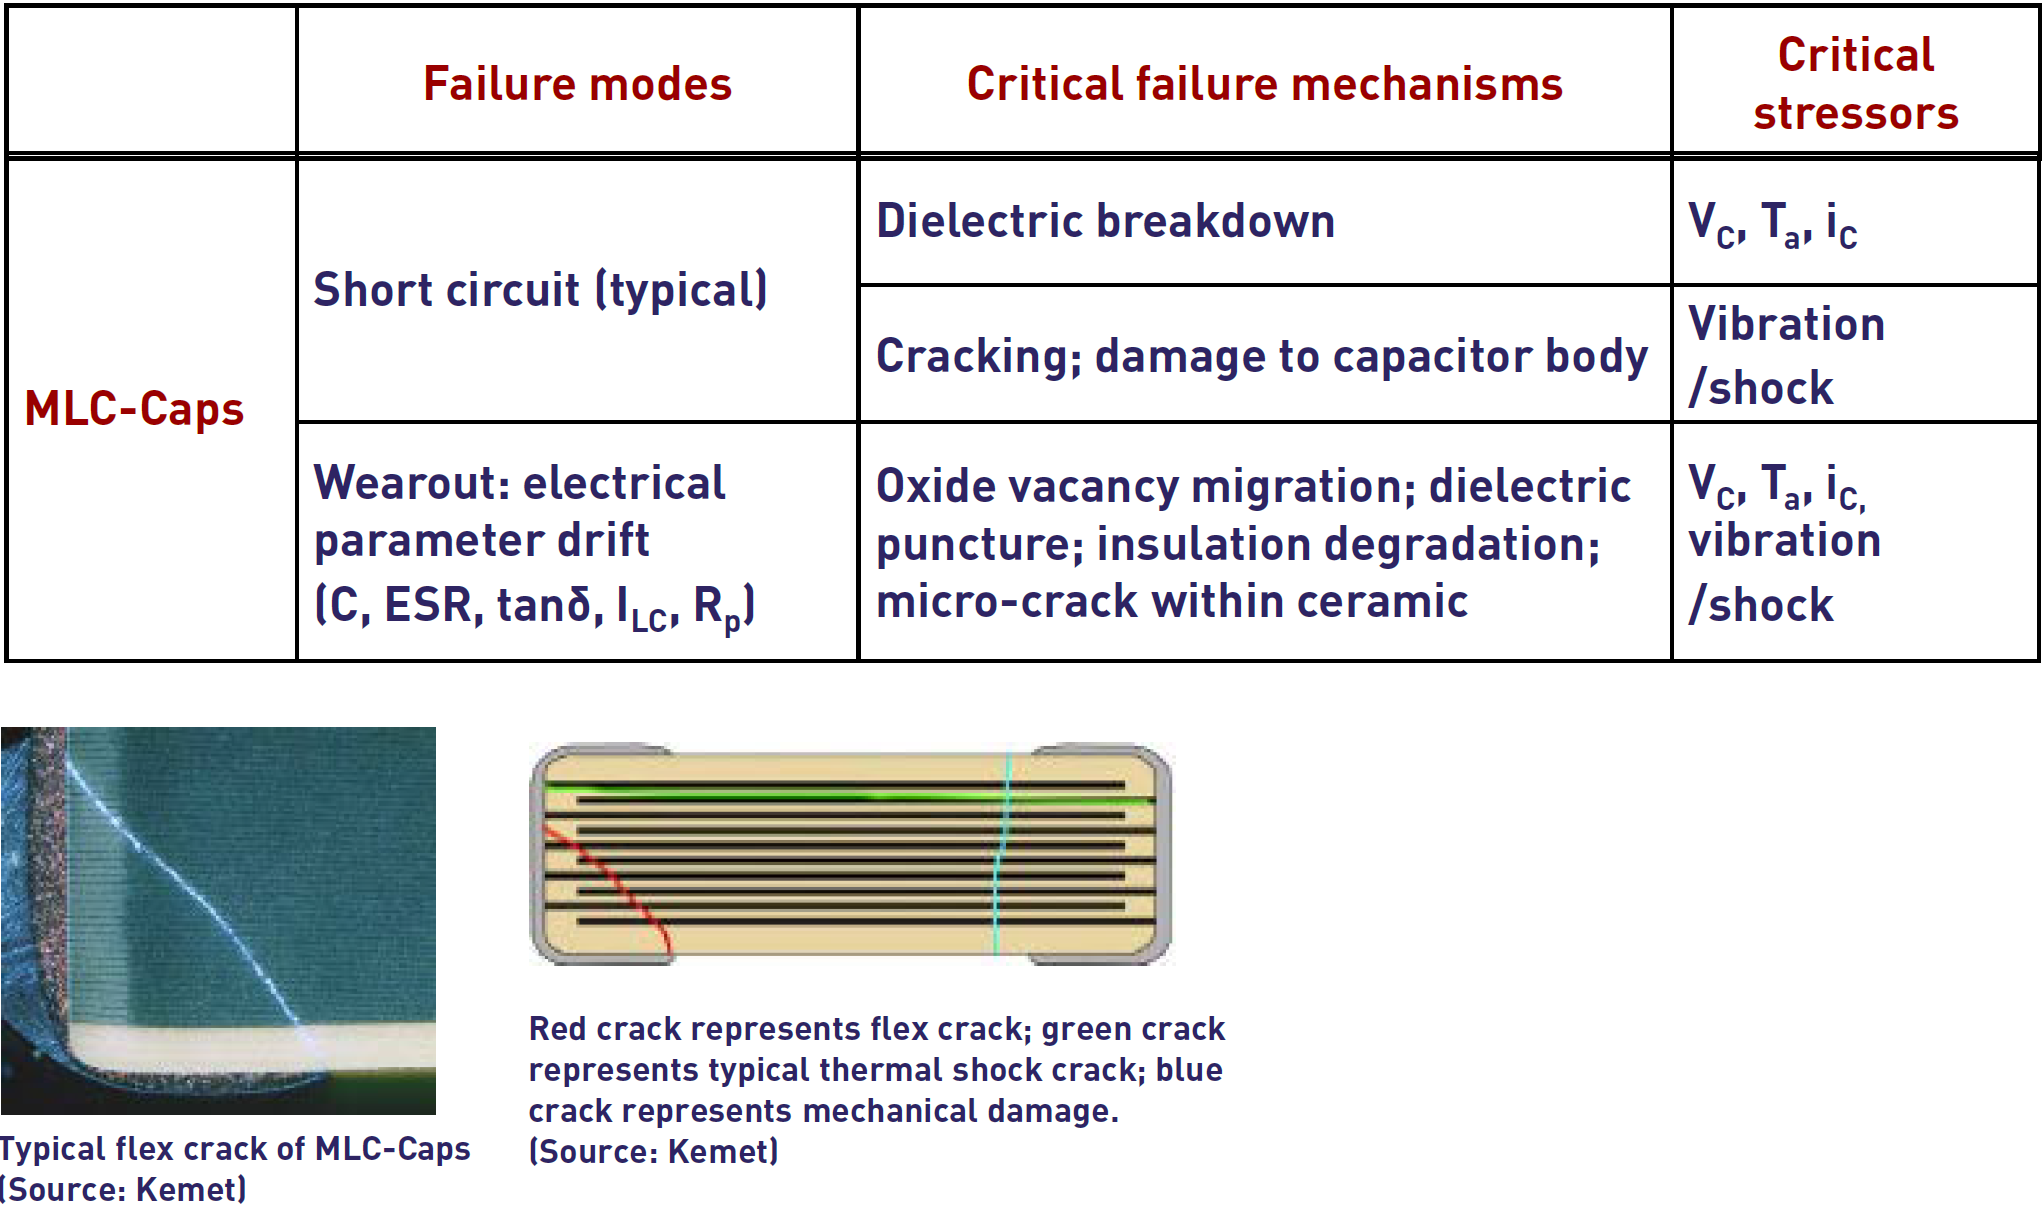
\includegraphics[width=\linewidth]{fig/lec08/MLCC_failure_modes.png}
    \caption{Failure modes, mechanisms, and critical stressors of multilayer ceramic capacitors, including flex and thermal-shock cracking. Adapted from Huai Wang, \textit{Capacitors in Power Electronics Applications -- Reliability and Circuit Design}, IECON 2016 tutorial}
\end{figure}
\end{column}
\end{columns}
\end{frame}


%%%%%%%%%%%%%%%%%%%%%%%%%%%%%%%%%%%%%%%%%%%%%%%%%%%%%%%%%%%%%
%% Failure mode comparison
%%%%%%%%%%%%%%%%%%%%%%%%%%%%%%%%%%%%%%%%%%%%%%%%%%%%%%%%%%%%%
\begin{frame}
\frametitle{Comparison of Failure Behaviour}

\begin{columns}
\begin{column}{0.6\textwidth}
Capacitors age and fail differently.
\begin{itemize}
    \item \textbf{Aluminum electrolytic capacitors}
    \begin{itemize}
        \item dominant failure mode: wear-out,
        \item typical failure: open circuit or parameter drift,
        \item critical stressors: temperature, voltage, ripple current.
    \end{itemize}

    \item \textbf{Metallized film capacitors}
    \begin{itemize}
        \item dominant failure mode: open circuit or capacitance loss,
        \item self-healing capability is good,
        \item critical stressors: humidity, voltage, temperature, ripple current.
    \end{itemize}

    \item \textbf{MLCCs}
    \begin{itemize}
        \item dominant failure mode: short circuit,
        \item no self-healing capability,
        \item critical stressors: voltage, temperature, vibration, shock and board flex.
    \end{itemize}
\end{itemize}

\end{column}

\begin{column}{0.40\textwidth}
\begin{figure}
    \centering
    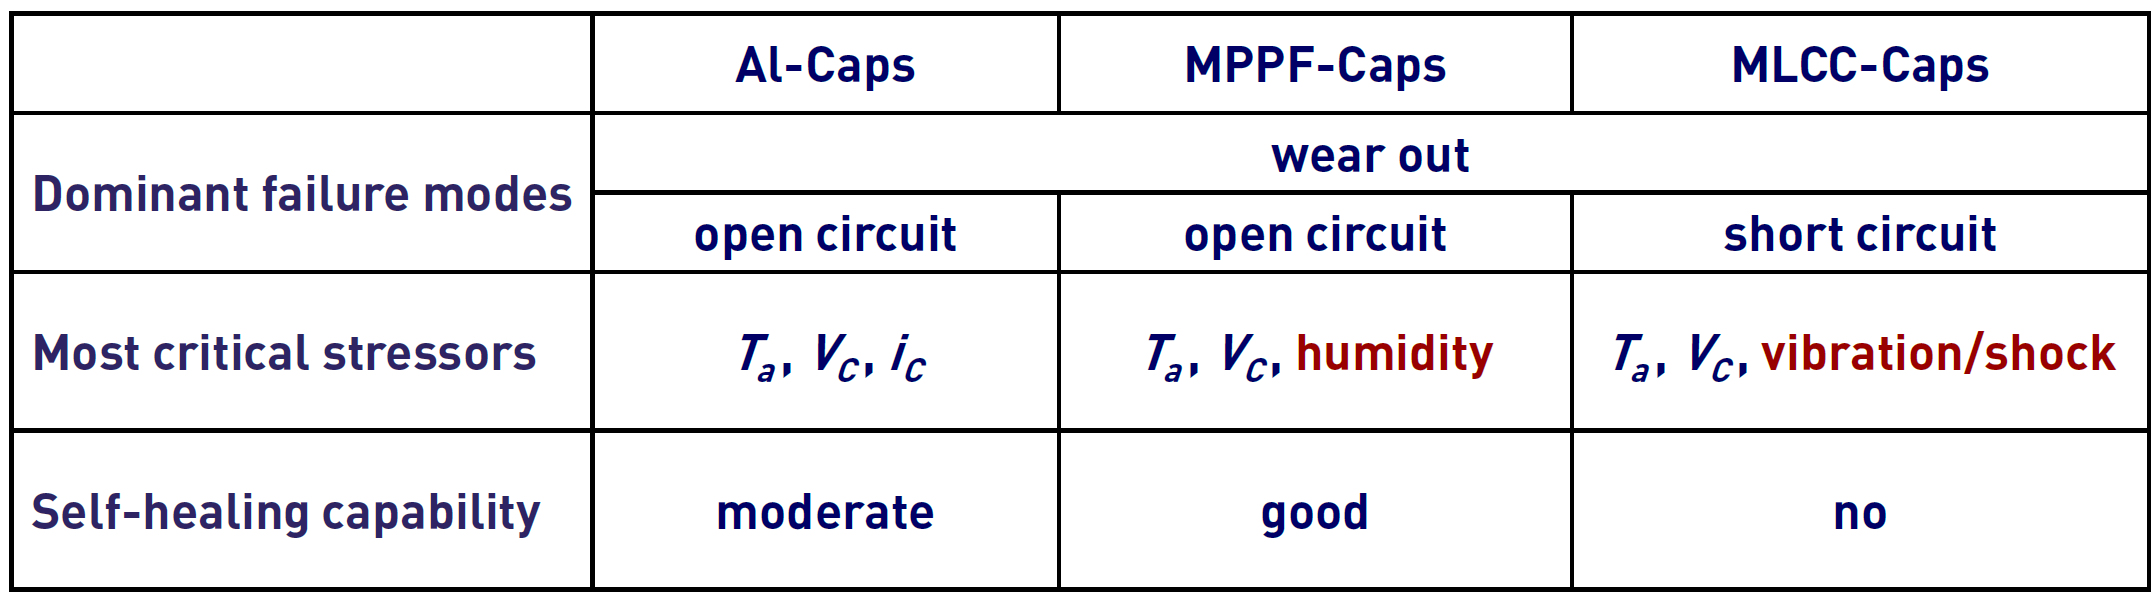
\includegraphics[width=\linewidth]{fig/lec08/failure_summary.png}
    \caption{Summary of dominant failure modes, critical stressors, and self-healing capability for aluminum electrolytic, metallized polypropylene film, and MLCC capacitors. Adapted from Huai Wang, \textit{Capacitors in Power Electronics Applications -- Reliability and Circuit Design}, IECON 2016 tutorial}
\end{figure}
\end{column}
\end{columns}

\end{frame}


%%%%%%%%%%%%%%%%%%%%%%%%%%%%%%%%%%%%%%%%%%%%%%%%%%%%%%%%%%%%%
%% Mission profile based analysis
%%%%%%%%%%%%%%%%%%%%%%%%%%%%%%%%%%%%%%%%%%%%%%%%%%%%%%%%%%%%%
\begin{frame}
\frametitle{Mission-Profile-Based Electro-Thermal Stress Analysis}
\begin{columns}
\begin{column}{0.56\textwidth}
A capacitor does not operate at one fixed condition during its lifetime. It experiences a mission profile. The mission profile includes:
\begin{itemize}
    \item ambient temperature variation,
    \item load power variation,
    \item input voltage variation,
    \item solar irradiance or wind-speed variation,
    \item start--stop cycles,
    \item overload and transient events.
\end{itemize}
\end{column}

\begin{column}{0.40\textwidth}
\begin{figure}
    \centering
    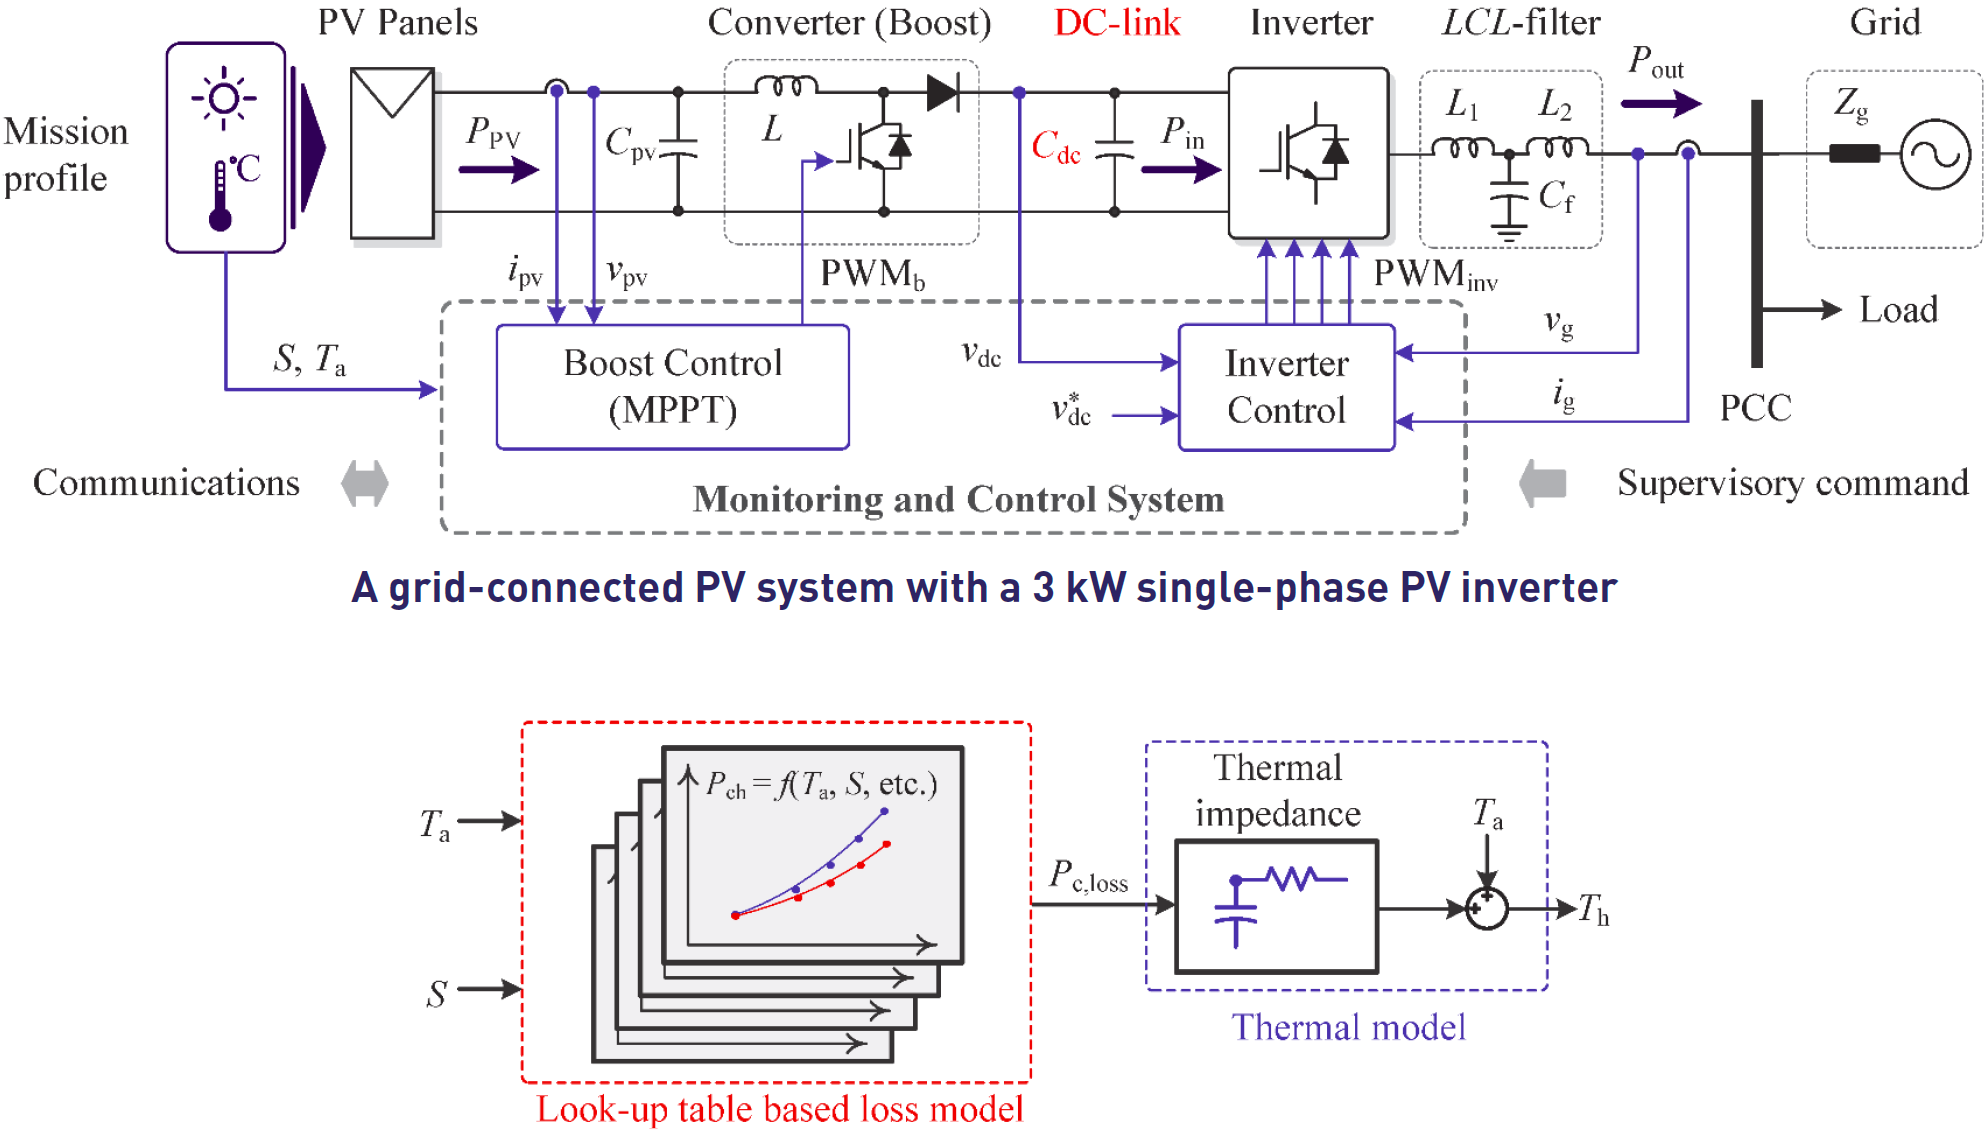
\includegraphics[width=\linewidth]{fig/lec08/mission_profile_model.png}
    \caption{Mission-profile-based electro-thermal modelling workflow for a single-phase PV inverter. Adapted from Huai Wang, \textit{Capacitors in Power Electronics Applications -- Reliability and Circuit Design}, IECON 2016 tutorial}
\end{figure}
\end{column}
\end{columns}

\end{frame}


%%%%%%%%%%%%%%%%%%%%%%%%%%%%%%%%%%%%%%%%%%%%%%%%%%%%%%%%%%%%%
%% Mission profile based analysis
%%%%%%%%%%%%%%%%%%%%%%%%%%%%%%%%%%%%%%%%%%%%%%%%%%%%%%%%%%%%%
\begin{frame}
\frametitle{Mission-Profile-Based Electro-Thermal Stress Analysis}
\begin{columns}
\begin{column}{0.56\textwidth}
The reliability-oriented workflow is:
\begin{enumerate}
    \item translate mission profile into capacitor voltage and current stress,
    \item calculate capacitor losses,
    \item estimate hot-spot temperature,
    \item apply ageing or lifetime model,
    \item accumulate damage over the mission profile.
\end{enumerate}
This approach is essential for PV inverters, EV chargers, railway converters, aircraft systems, and wind-power converters.
\end{column}

\begin{column}{0.40\textwidth}
\begin{figure}
    \centering
    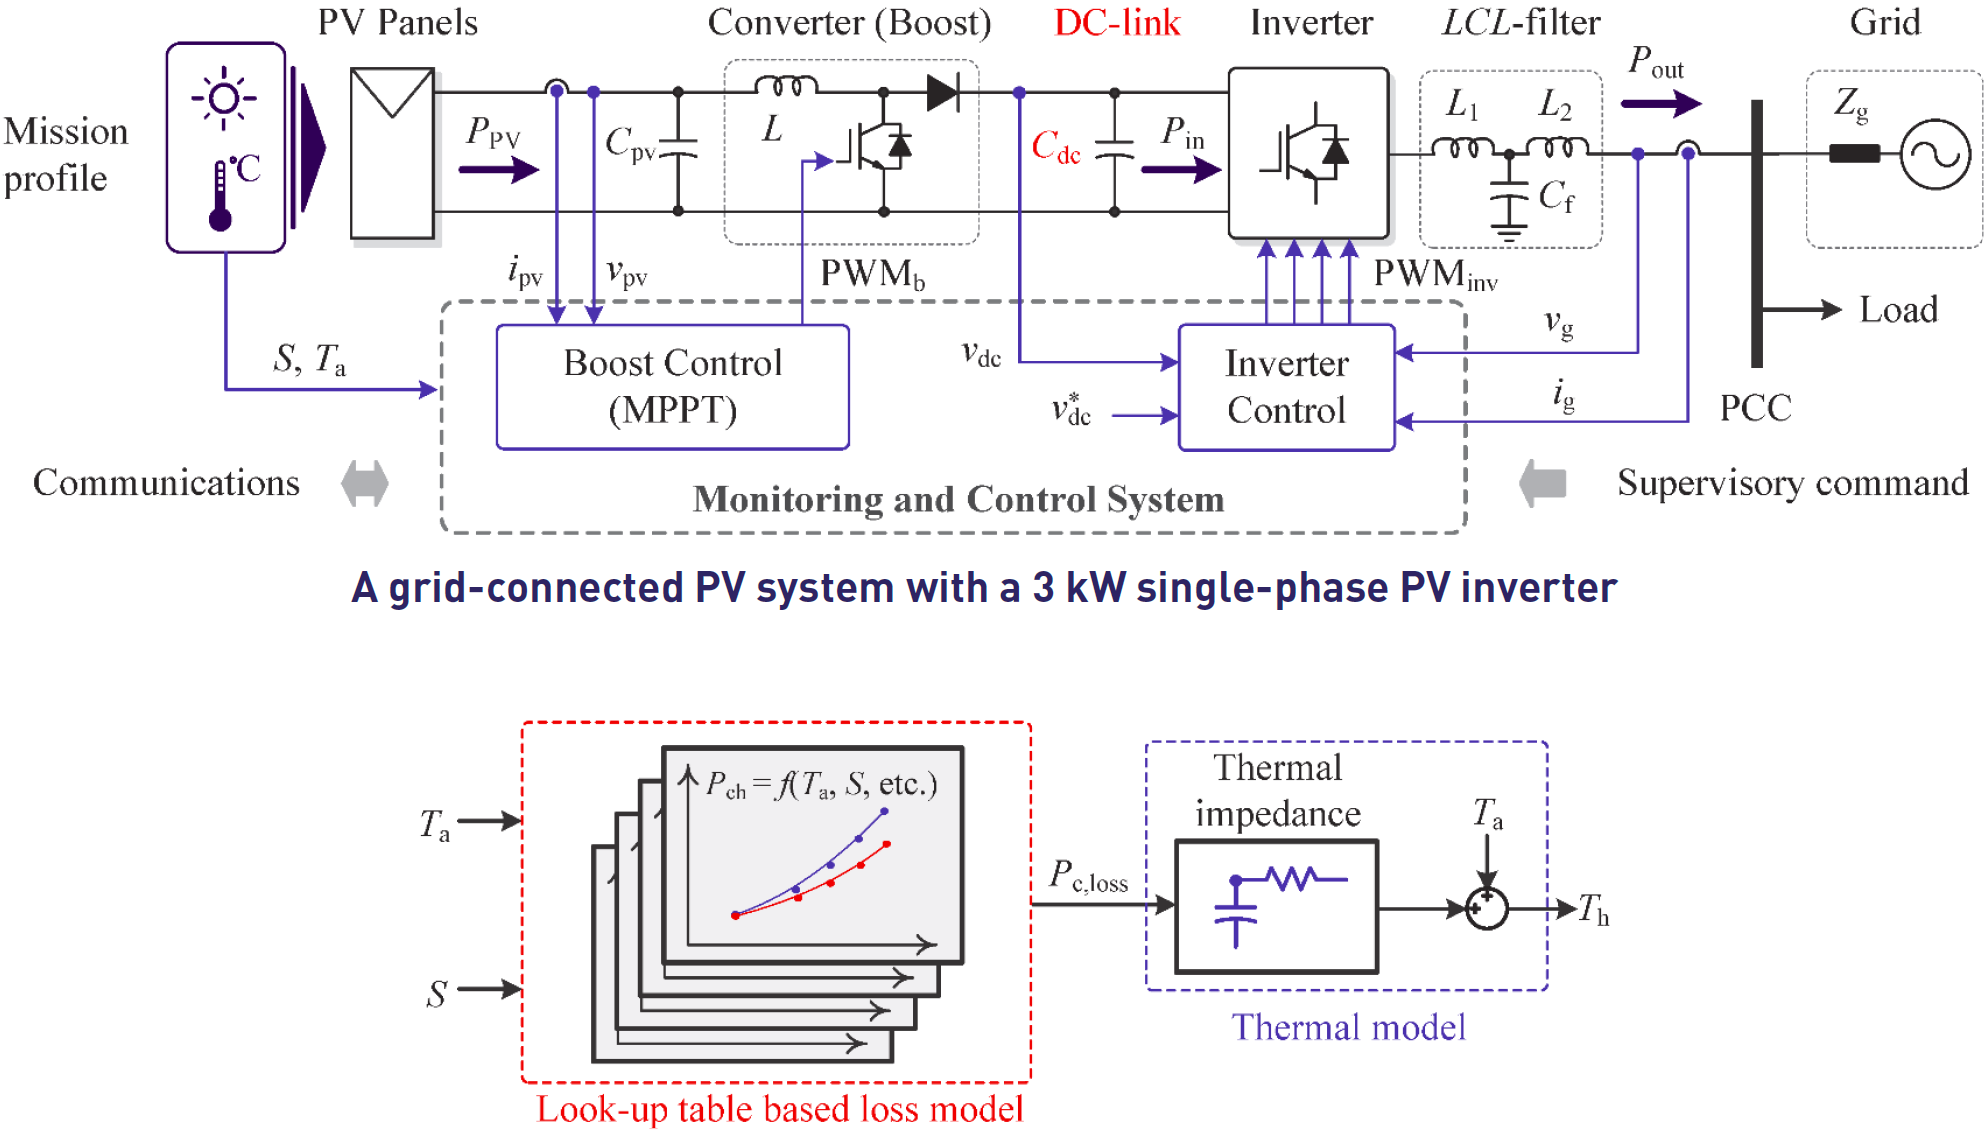
\includegraphics[width=\linewidth]{fig/lec08/mission_profile_model.png}
    \caption{Mission-profile-based electro-thermal modelling workflow for a single-phase PV inverter. Adapted from Huai Wang, \textit{Capacitors in Power Electronics Applications -- Reliability and Circuit Design}, IECON 2016 tutorial}
\end{figure}
\end{column}
\end{columns}

\end{frame}

%%%%%%%%%%%%%%%%%%%%%%%%%%%%%%%%%%%%%%%%%%%%%%%%%%%%%%%%%%%%%
%% Ripple spectrum and temperature stress
%%%%%%%%%%%%%%%%%%%%%%%%%%%%%%%%%%%%%%%%%%%%%%%%%%%%%%%%%%%%%
\begin{frame}
\frametitle{Ripple-Current Spectrum and Temperature Stress}
\begin{columns}
\begin{column}{0.56\textwidth}
In power converters, capacitor current is rarely sinusoidal. It contains many harmonic components. For harmonic currents,

\begin{align}
    I_{\mathrm{rms}}
    =
    \sqrt{
    I_1^2+I_2^2+\cdots+I_n^2
    }
\end{align}

The loss is frequency dependent because ESR changes with frequency:

\begin{align}
    P_{\mathrm{loss}}
    =
    \sum_{k=1}^{n}
    I_k^2
    ESR(f_k)
\end{align}
\end{column}

\begin{column}{0.40\textwidth}
\begin{figure}
    \centering
    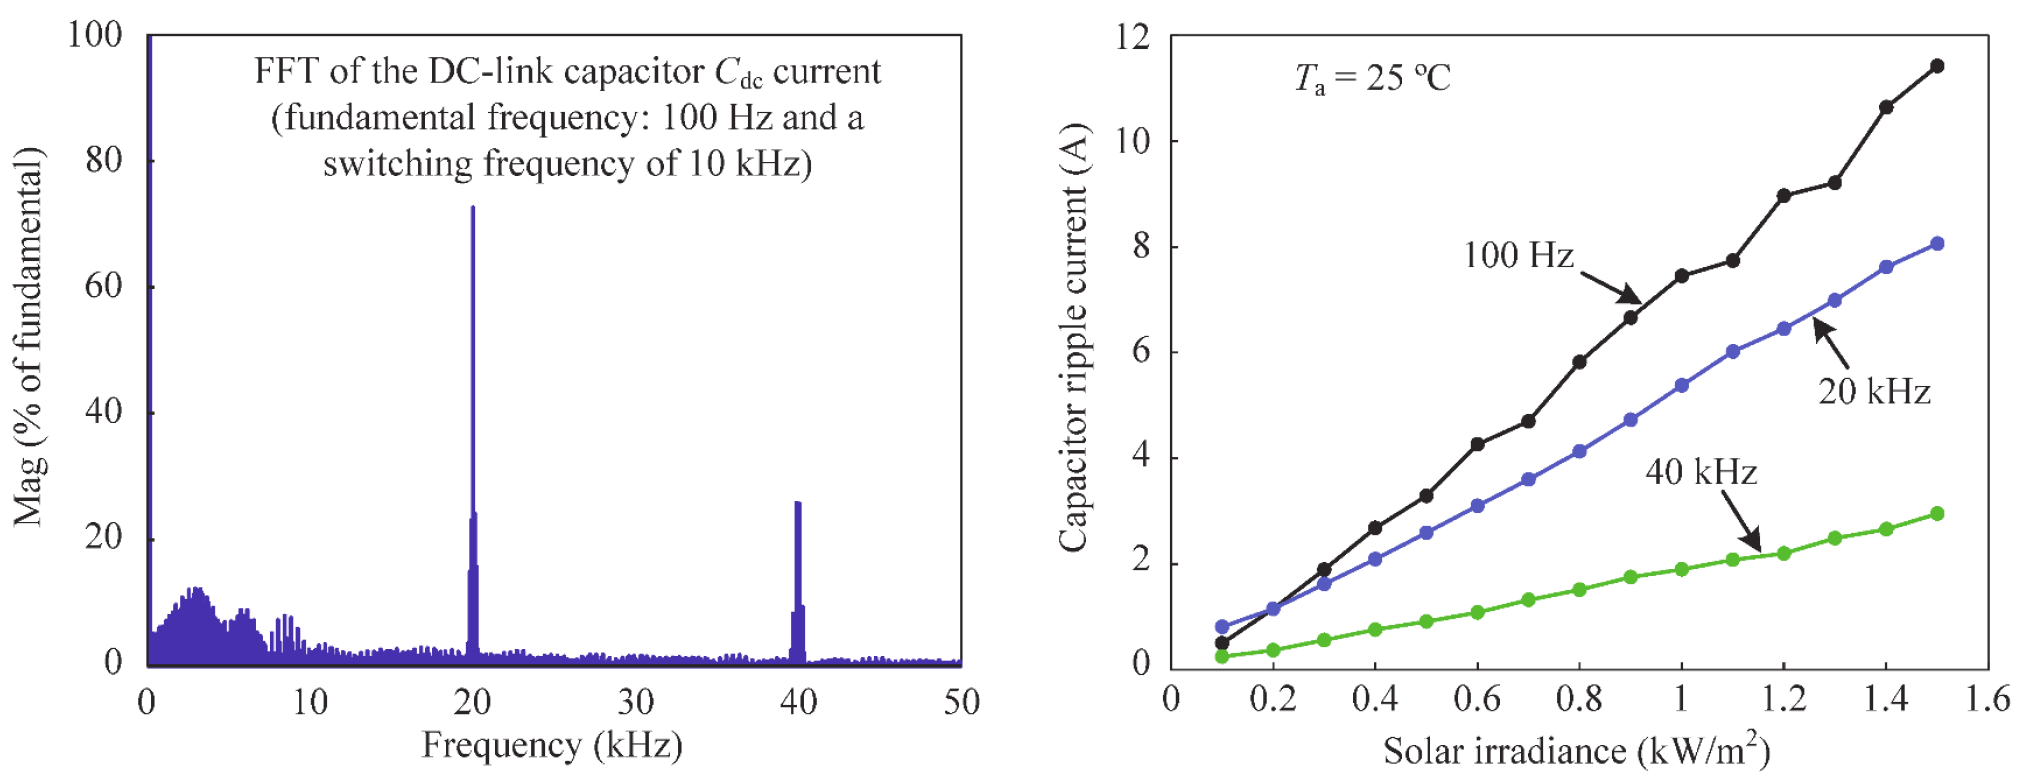
\includegraphics[width=\linewidth]{fig/lec08/ripple_current_spectrum.png}
    \caption{Example ripple-current harmonic spectrum and capacitor ripple currents under different irradiance levels. Adapted from Huai Wang, \textit{Capacitors in Power Electronics Applications -- Reliability and Circuit Design}, IECON 2016 tutorial}
\end{figure}
\end{column}
\end{columns}

\end{frame}


%%%%%%%%%%%%%%%%%%%%%%%%%%%%%%%%%%%%%%%%%%%%%%%%%%%%%%%%%%%%%
%% Ripple spectrum and temperature stress
%%%%%%%%%%%%%%%%%%%%%%%%%%%%%%%%%%%%%%%%%%%%%%%%%%%%%%%%%%%%%
\begin{frame}
\frametitle{Ripple-Current Spectrum and Temperature Stress}
\begin{columns}
\begin{column}{0.56\textwidth}
Ripple spectrum and temperature stress are especially important for:
\begin{itemize}
    \item DC-link capacitors in inverters,
    \item output capacitors in DC--DC converters,
    \item resonant capacitors,
    \item EMI and AC harmonic filter capacitors.
\end{itemize}
A single RMS current number may be insufficient if the frequency spectrum is broad.
\end{column}

\begin{column}{0.40\textwidth}
\begin{figure}
    \centering
    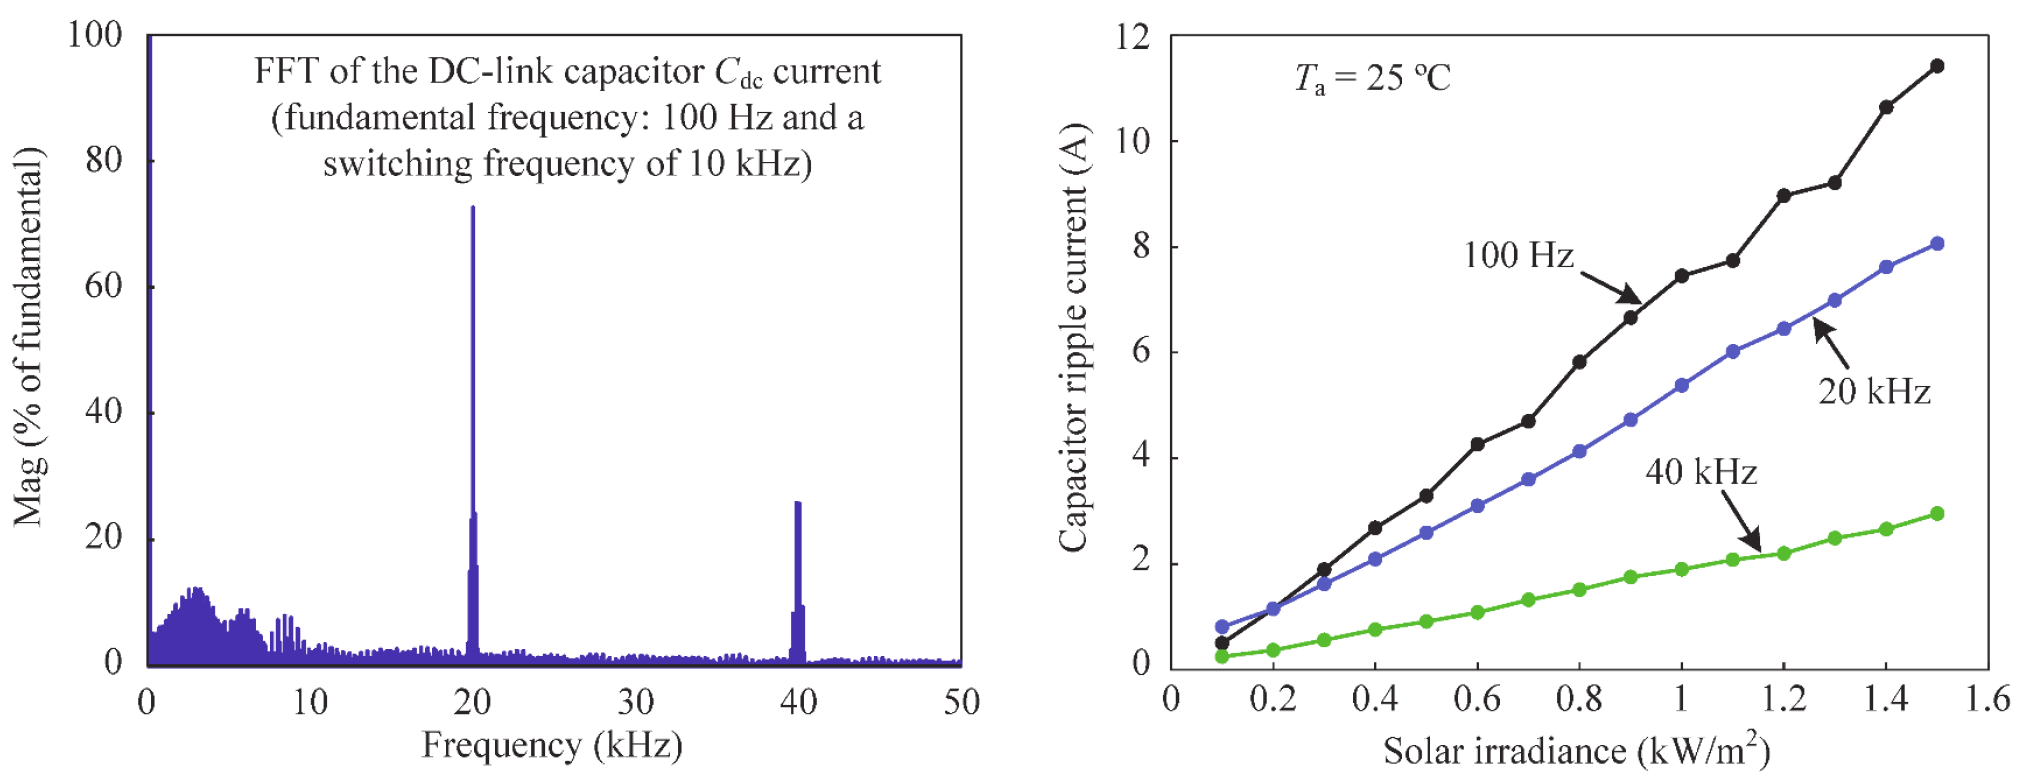
\includegraphics[width=\linewidth]{fig/lec08/ripple_current_spectrum.png}
    \caption{Example ripple-current harmonic spectrum and capacitor ripple currents under different irradiance levels. Adapted from Huai Wang, \textit{Capacitors in Power Electronics Applications -- Reliability and Circuit Design}, IECON 2016 tutorial}
\end{figure}
\end{column}
\end{columns}

\end{frame}

%%%%%%%%%%%%%%%%%%%%%%%%%%%%%%%%%%%%%%%%%%%%%%%%%%%%%%%%%%%%%
%% Humidity degradation film capacitors
%%%%%%%%%%%%%%%%%%%%%%%%%%%%%%%%%%%%%%%%%%%%%%%%%%%%%%%%%%%%%
\begin{frame}
\frametitle{Humidity-Dependent Degradation of Film Capacitors}

\begin{columns}
\begin{column}{0.60\textwidth}
Metallized film capacitors are sensitive to humidity because moisture can degrade the metallization layer. The main effects are:
\begin{itemize}
    \item reduction of active electrode area,
    \item capacitance decrease,
    \item increased dielectric loss,
    \item self-healing activity,
    \item gradual wear-out.
\end{itemize}
In accelerated tests, end-of-life can be defined by a specified capacitance drop, for example \(5\%\) reduction.

For PV inverters and outdoor converters, humidity stress must be considered with voltage, temperature, and ripple current.
\end{column}

\begin{column}{0.40\textwidth}
        \vspace{-0.5cm}
\begin{figure}
    \centering
    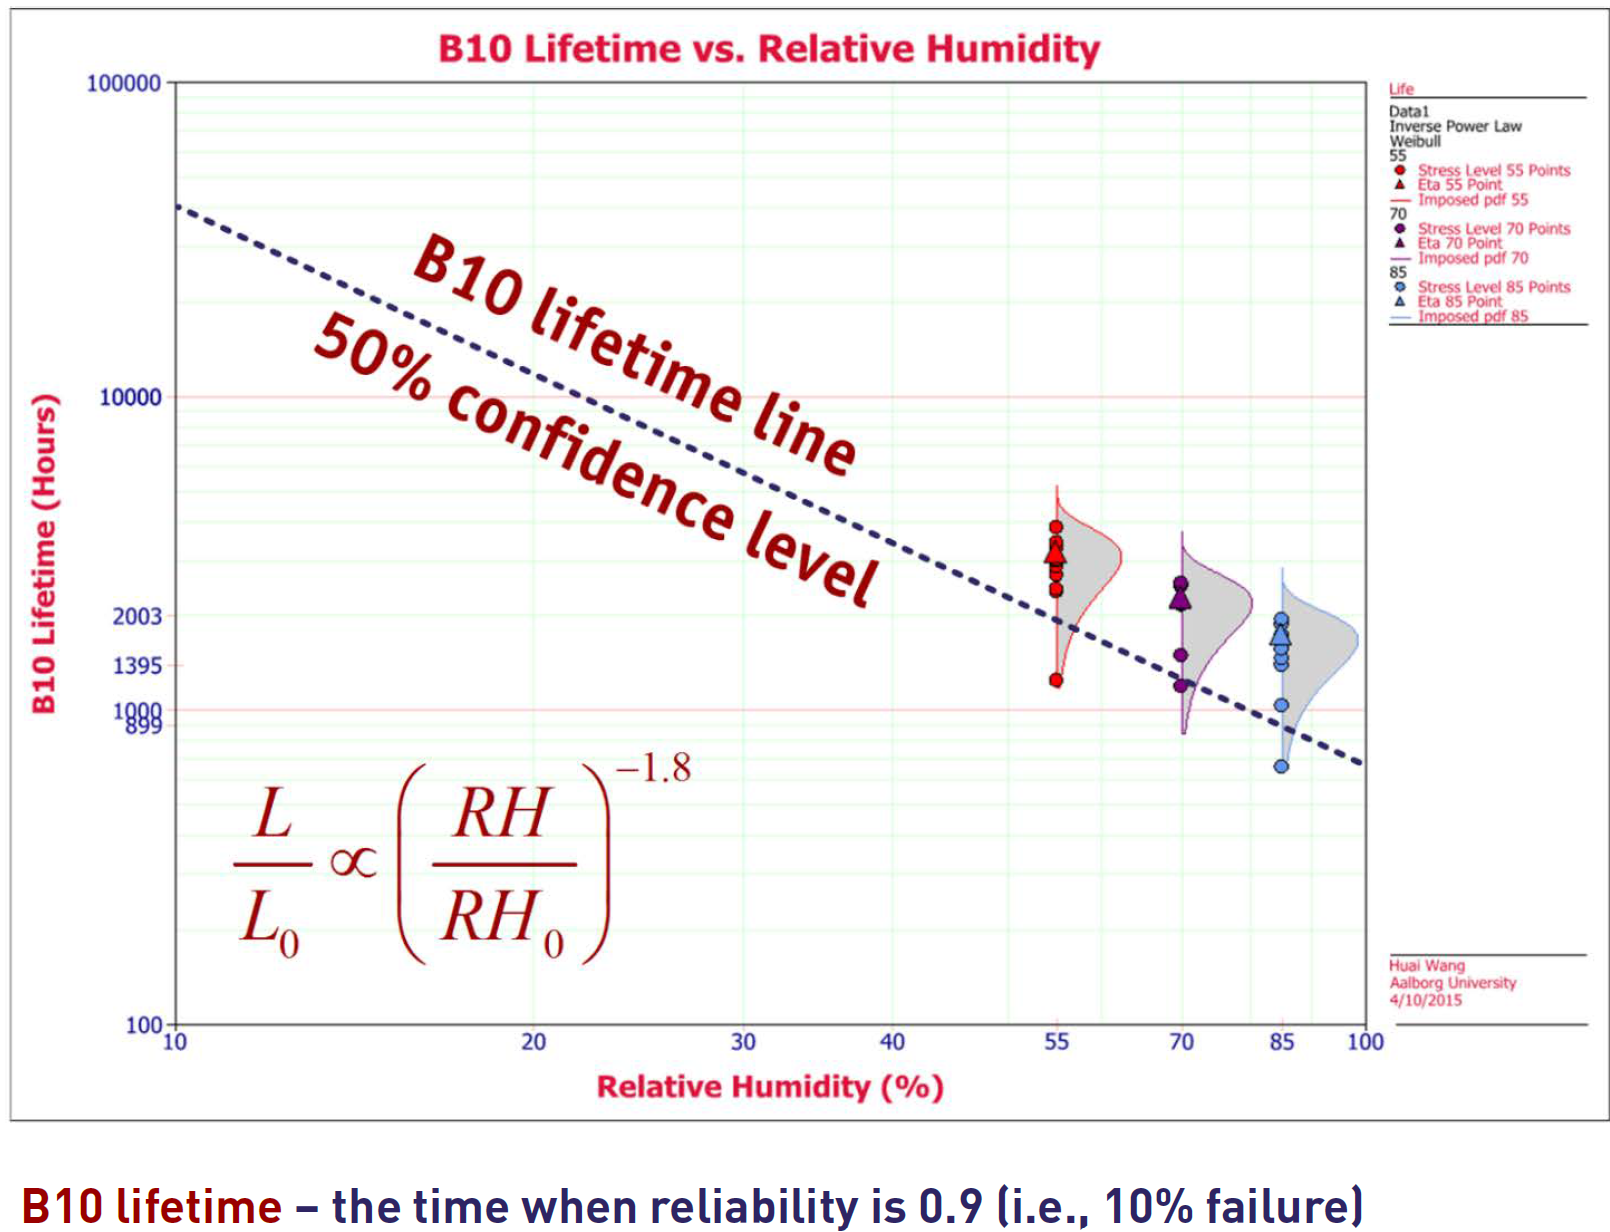
\includegraphics[width=\linewidth]{fig/lec08/humidity_lifetime_MPPF.png}
    \caption{Humidity-dependent lifetime of metallized polypropylene film capacitors under accelerated ageing conditions. Adapted from Huai Wang, \textit{Capacitors in Power Electronics Applications -- Reliability and Circuit Design}, IECON 2016 tutorial}
\end{figure}
\end{column}
\end{columns}

\end{frame}


%%%%%%%%%%%%%%%%%%%%%%%%%%%%%%%%%%%%%%%%%%%%%%%%%%%%%%%%%%%%%
%% Condition monitoring
%%%%%%%%%%%%%%%%%%%%%%%%%%%%%%%%%%%%%%%%%%%%%%%%%%%%%%%%%%%%%
\begin{frame}
\frametitle{Condition Monitoring of Capacitors}
\begin{columns}
\begin{column}{0.56\textwidth}
Condition monitoring aims to estimate the health of a capacitor during converter operation.Useful health indicators include:
\begin{itemize}
    \item capacitance \(C\),
    \item ESR,
    \item dissipation factor \(\tan\delta\),
    \item leakage current \(I_{\mathrm{LC}}\),
    \item insulation resistance \(R_p\),
    \item hot-spot temperature,
    \item ripple-current stress.
\end{itemize}
\end{column}

\begin{column}{0.45\textwidth}
        \vspace{-1cm}
\begin{figure}
    \centering
    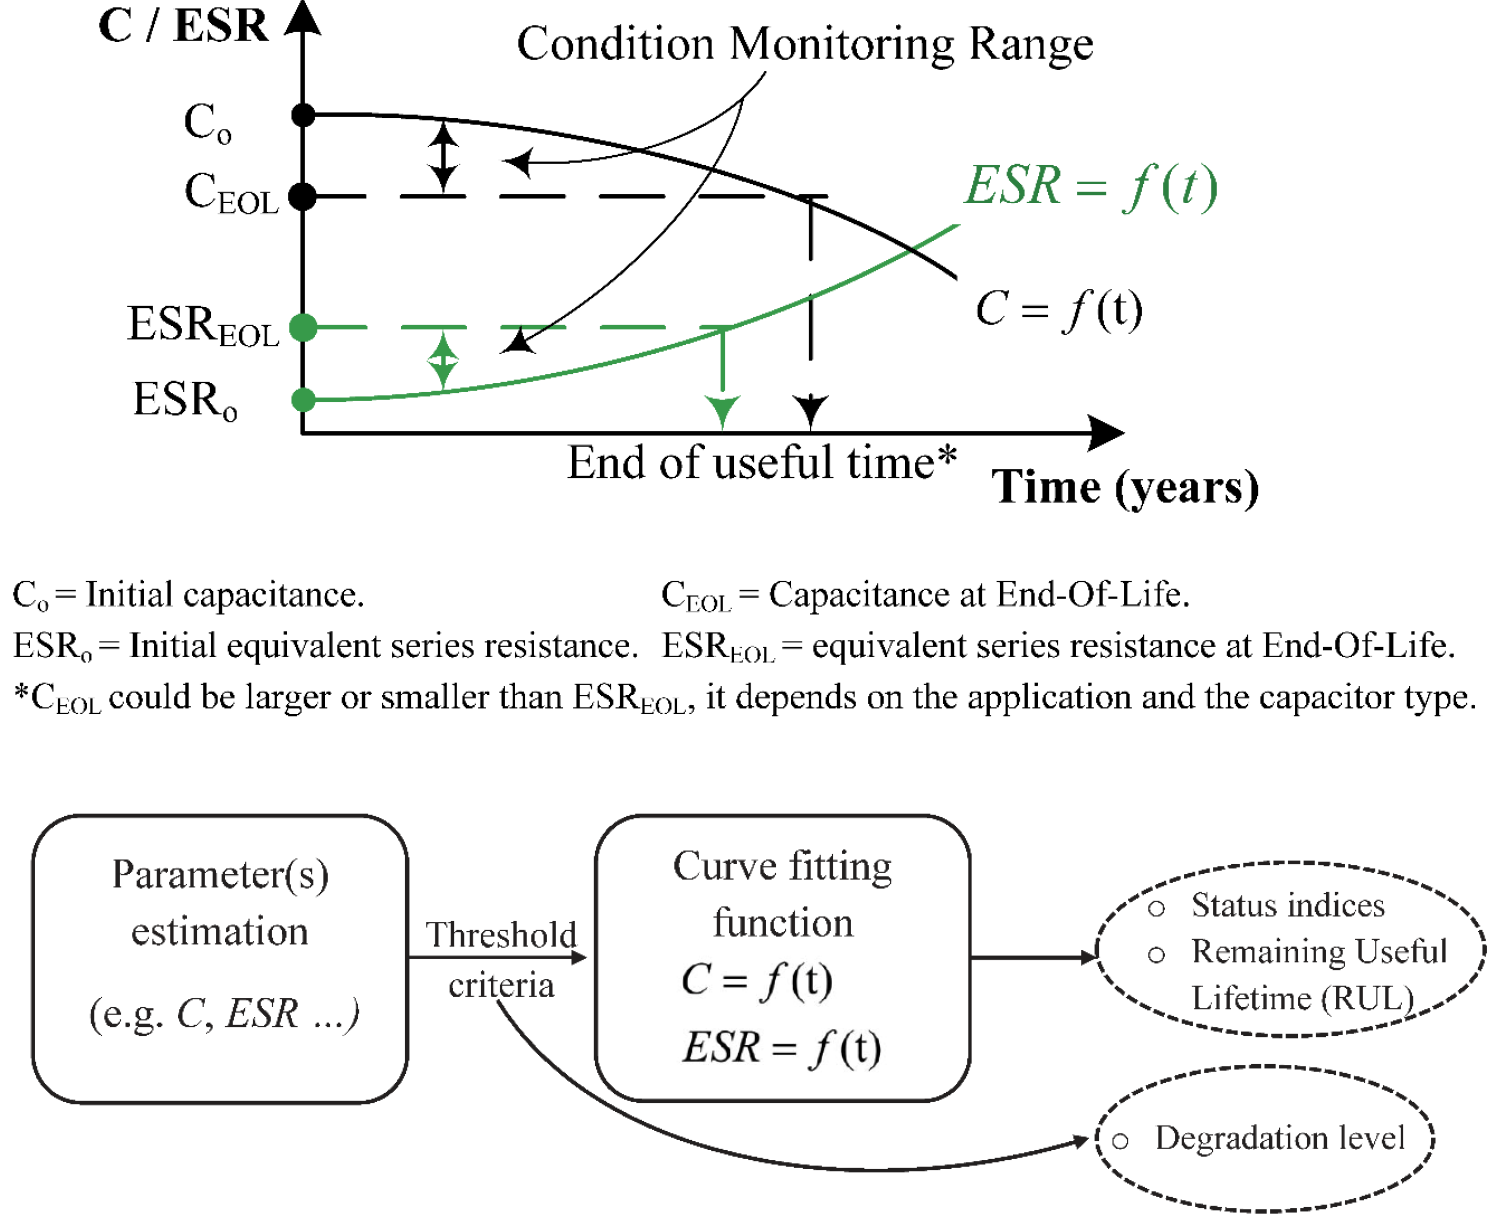
\includegraphics[width=\linewidth]{fig/lec08/condition_indicators.png}
    \caption{Key indicators for capacitor condition monitoring: capacitance, ESR, \(\tan\delta\), leakage current and insulation resistance. Adapted from Huai Wang, \textit{Capacitors in Power Electronics Applications -- Reliability and Circuit Design}, IECON 2016 tutorial}
\end{figure}
\end{column}
\end{columns}

\end{frame}


%%%%%%%%%%%%%%%%%%%%%%%%%%%%%%%%%%%%%%%%%%%%%%%%%%%%%%%%%%%%%
%% Condition monitoring
%%%%%%%%%%%%%%%%%%%%%%%%%%%%%%%%%%%%%%%%%%%%%%%%%%%%%%%%%%%%%
\begin{frame}
\frametitle{Condition Monitoring of Capacitors}
\begin{columns}
\begin{column}{0.56\textwidth}
Typical ageing trends:
\begin{itemize}
    \item electrolytic capacitors: ESR increases and capacitance decreases,
    \item film capacitors: capacitance decreases due to metallization loss,
    \item MLCCs: insulation degradation or cracking may produce sudden failure.
\end{itemize}
Online monitoring is particularly valuable for DC-link capacitors in long-life converters.

\end{column}

\begin{column}{0.45\textwidth}
    \vspace{-1cm}
\begin{figure}
    \centering
    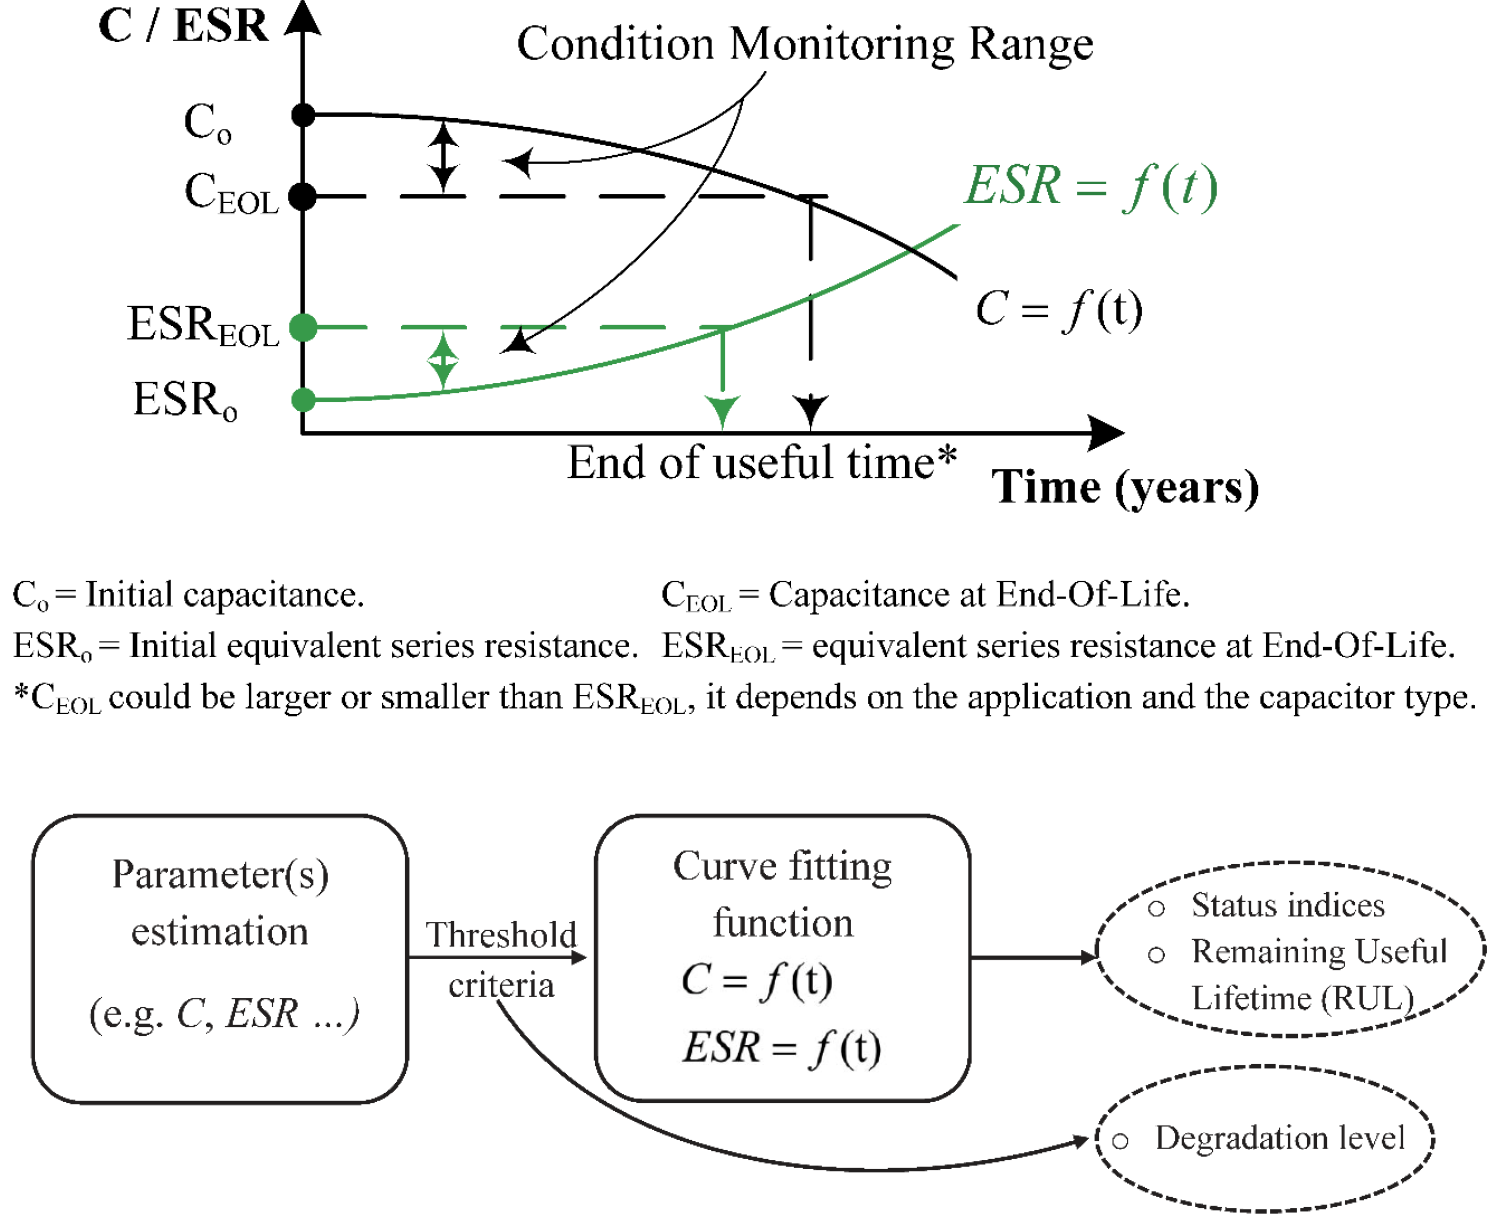
\includegraphics[width=\linewidth]{fig/lec08/condition_indicators.png}
    \caption{Key indicators for capacitor condition monitoring: capacitance, ESR, \(\tan\delta\), leakage current and insulation resistance. Adapted from Huai Wang, \textit{Capacitors in Power Electronics Applications -- Reliability and Circuit Design}, IECON 2016 tutorial}
\end{figure}
\end{column}
\end{columns}

\end{frame}

%%%%%%%%%%%%%%%%%%%%%%%%%%%%%%%%%%%%%%%%%%%%%%%%%%%%%%%%%%%%%
%% ESR estimation
%%%%%%%%%%%%%%%%%%%%%%%%%%%%%%%%%%%%%%%%%%%%%%%%%%%%%%%%%%%%%
\begin{frame}
\frametitle{Online ESR Estimation}
\begin{columns}
\begin{column}{0.56\textwidth}
A common online health-monitoring method estimates the ESR of the DC-link capacitor. The basic idea is that ESR creates a voltage ripple proportional to capacitor current:

\begin{align}
    v_{\mathrm{ESR}}(t)
    =
    i_C(t)R_{\mathrm{ESR}}
\end{align}
Thus, if capacitor current and ripple voltage are known or estimated,
\begin{align}
    R_{\mathrm{ESR}}
    \approx
    \frac{v_{\mathrm{ripple}}}{i_{\mathrm{ripple}}}
\end{align}
\end{column}

\begin{column}{0.40\textwidth}
\begin{figure}
    \centering
    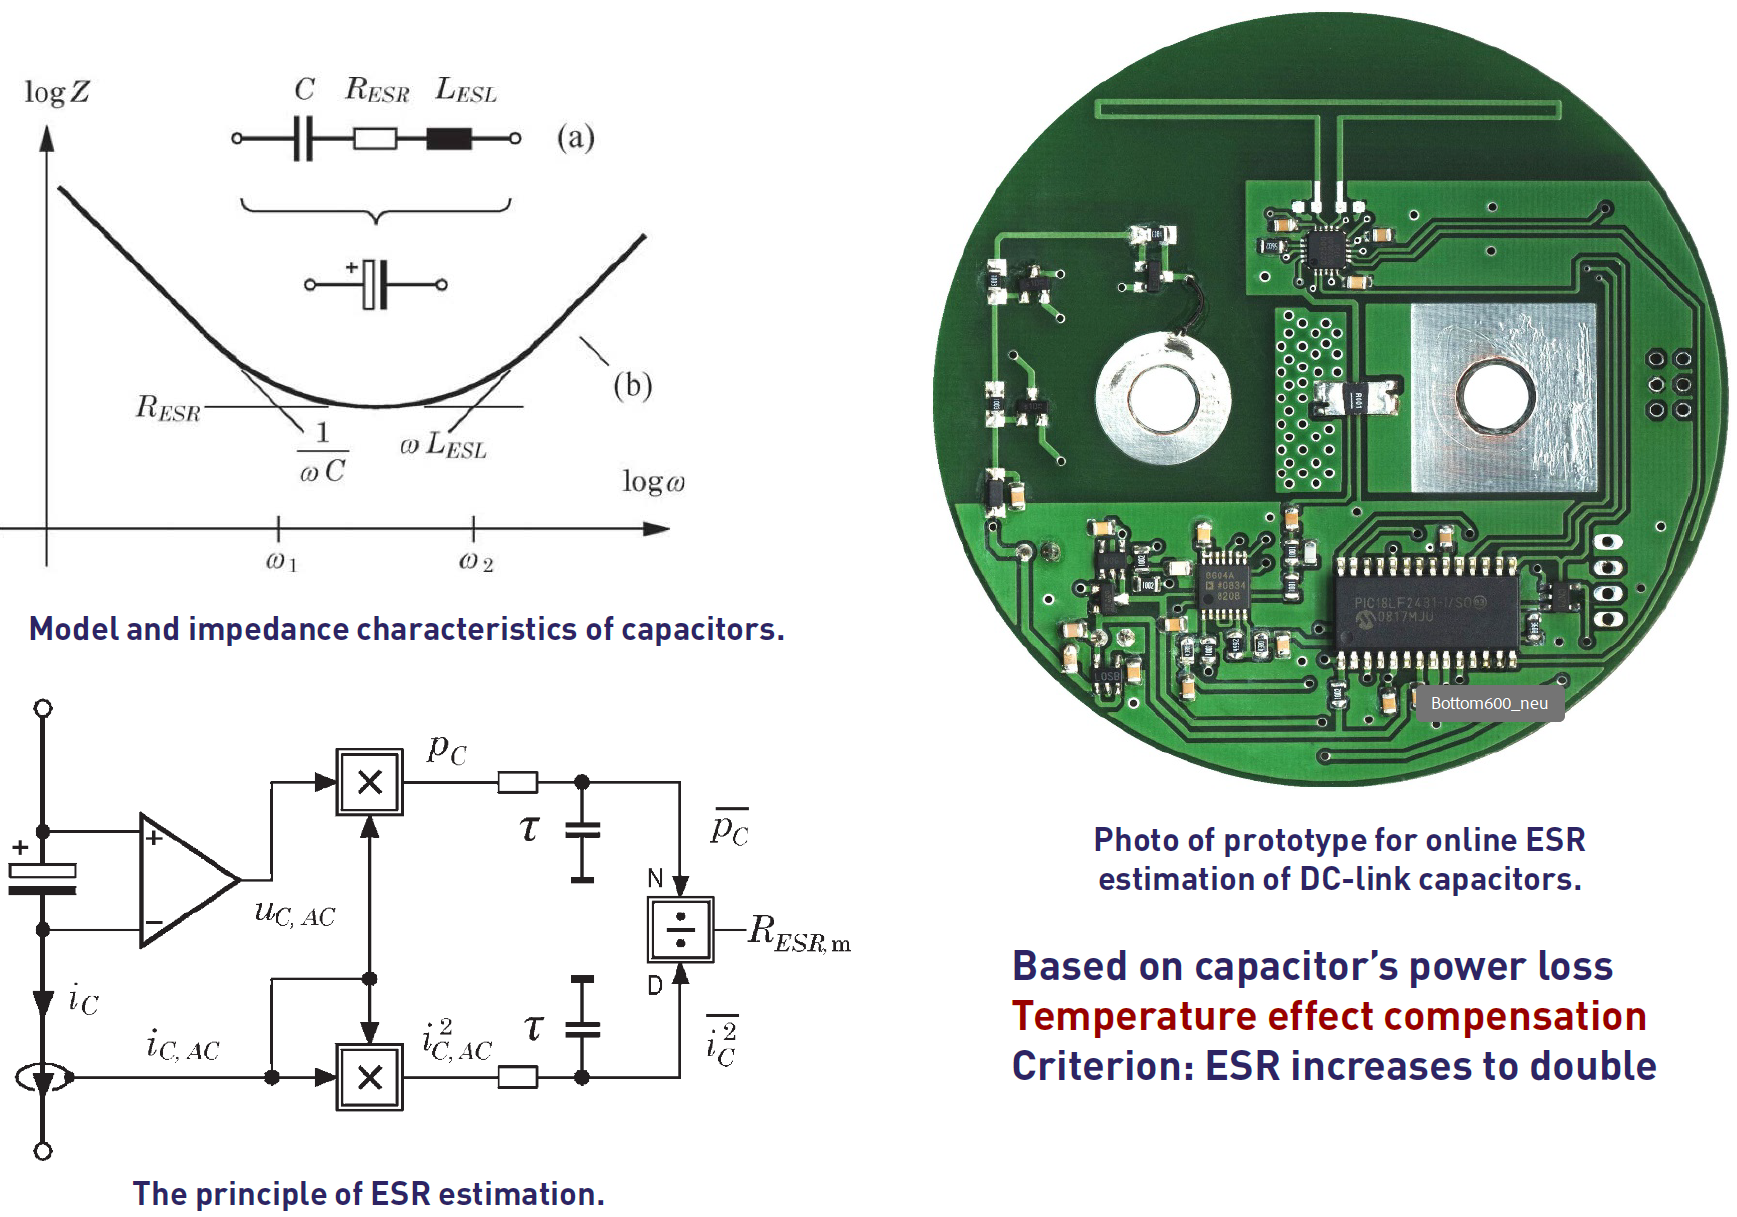
\includegraphics[width=\linewidth]{fig/lec08/online_ESR_estimation.png}
    \caption{Prototype and principle for online ESR estimation of DC-link capacitors, including temperature compensation. Adapted from Huai Wang, \textit{Capacitors in Power Electronics Applications -- Reliability and Circuit Design}, IECON 2016 tutorial}
\end{figure}
\end{column}
\end{columns}

\end{frame}


%%%%%%%%%%%%%%%%%%%%%%%%%%%%%%%%%%%%%%%%%%%%%%%%%%%%%%%%%%%%%
%% ESR estimation
%%%%%%%%%%%%%%%%%%%%%%%%%%%%%%%%%%%%%%%%%%%%%%%%%%%%%%%%%%%%%
\begin{frame}
\frametitle{Online ESR Estimation}
\begin{columns}
\begin{column}{0.56\textwidth}
However, practical ESR estimation must compensate for:
\begin{itemize}
    \item temperature dependence,
    \item frequency dependence,
    \item measurement noise,
    \item non-ESR ripple components,
    \item converter operating-point variation.
\end{itemize}
A typical end-of-life criterion for electrolytic capacitors is ESR increasing to a specified multiple of its initial value.
\end{column}

\begin{column}{0.40\textwidth}
\begin{figure}
    \centering
    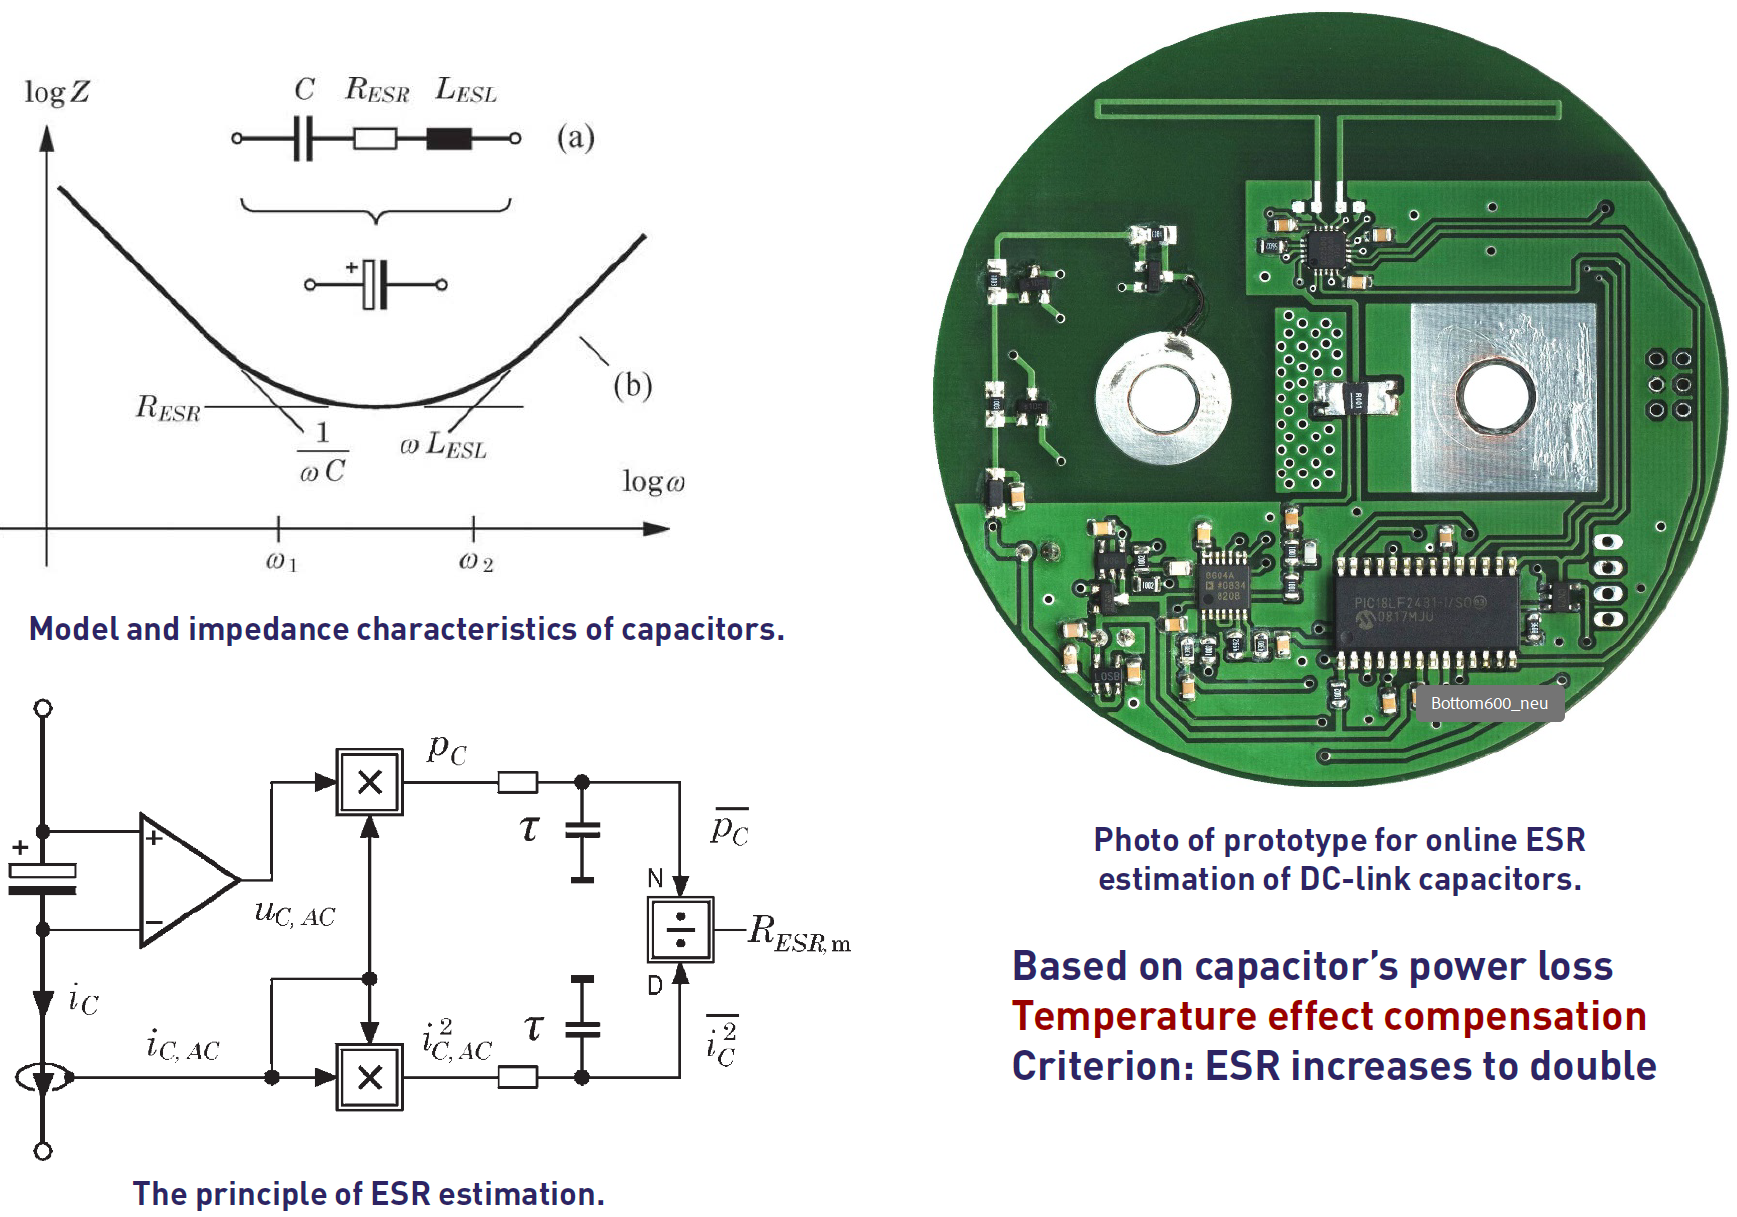
\includegraphics[width=\linewidth]{fig/lec08/online_ESR_estimation.png}
    \caption{Prototype and principle for online ESR estimation of DC-link capacitors, including temperature compensation. Adapted from Huai Wang, \textit{Capacitors in Power Electronics Applications -- Reliability and Circuit Design}, IECON 2016 tutorial}
\end{figure}
\end{column}
\end{columns}
\end{frame}


%%%%%%%%%%%%%%%%%%%%%%%%%%%%%%%%%%%%%%%%%%%%%%%%%%%%%%%%%%%%%
%% Remaining lifetime prediction
%%%%%%%%%%%%%%%%%%%%%%%%%%%%%%%%%%%%%%%%%%%%%%%%%%%%%%%%%%%%%
\begin{frame}
\frametitle{Remaining Lifetime Prediction}
Remaining lifetime prediction combines condition monitoring with ageing models. A general workflow is:

\begin{enumerate}
    \item measure or estimate capacitor stress:
    \[
        V_C,\; i_C,\; T_{\mathrm{hotspot}}
    \]

    \item estimate health indicators:
    \[
        C,\; ESR,\; \tan\delta,\; I_{\mathrm{LC}}
    \]

    \item compare with degradation model,

    \item predict time to end-of-life criterion.
\end{enumerate}
Relevant for converters where capacitor replacement is expensive or difficult, such as:
\begin{itemize}
    \item offshore wind converters,
    \item railway converters,
    \item PV inverters,
    \item aircraft power systems,
    \item EV fast chargers.
\end{itemize}

\end{frame}


%%%%%%%%%%%%%%%%%%%%%%%%%%%%%%%%%%%%%%%%%%%%%%%%%%%%%%%%%%%%%
%% Common design mistakes
%%%%%%%%%%%%%%%%%%%%%%%%%%%%%%%%%%%%%%%%%%%%%%%%%%%%%%%%%%%%%
\begin{frame}
\frametitle{Common Capacitor Design Mistakes}

\begin{itemize}
    \item Selecting the capacitor only by nominal capacitance.

    \item Ignoring effective MLCC capacitance reduction under DC bias.

    \item Checking voltage rating but not ripple-current rating.

    \item Assuming RMS current sharing is equal in a parallel capacitor bank.

    \item Ignoring ESR variation with temperature, frequency and ageing.

    \item Ignoring ESL and external loop inductance in fast SiC/GaN converters.

    \item Using bulk electrolytics for high-frequency decoupling without local ceramic or film capacitors.

    \item Omitting discharge resistors or safe discharge verification in high-voltage DC links.

    \item Neglecting humidity effects in metallized film capacitors used in outdoor converters.

    \item Estimating lifetime from ambient temperature instead of capacitor hot-spot temperature.

    \item Ignoring mechanical stress, board flex, and cracking risk for MLCCs.
\end{itemize}

\end{frame}


%%%%%%%%%%%%%%%%%%%%%%%%%%%%%%%%%%%%%%%%%%%%%%%%%%%%%%%%%%%%%
%% Capacitors for WBG converters
%%%%%%%%%%%%%%%%%%%%%%%%%%%%%%%%%%%%%%%%%%%%%%%%%%%%%%%%%%%%%
\begin{frame}
\frametitle{Capacitors for SiC and GaN Power Electronics}
SiC and GaN devices enable high switching frequency and very fast voltage/current transitions. This changes capacitor requirements significantly. Important requirements are:

\begin{itemize}
    \item very low ESL,
    \item high RMS and peak current density,
    \item high \(dv/dt\) capability,
    \item high-temperature operation,
    \item compact placement close to the switching cell,
    \item low-loss operation at hundreds of kHz to MHz,
    \item compatibility with laminated busbars or embedded PCB structures.
\end{itemize}

The capacitor must be co-designed with the power module and layout. Otherwise, the switching speed advantage of WBG devices is lost to ringing, overshoot, EMI and thermal stress.

\end{frame}


%%%%%%%%%%%%%%%%%%%%%%%%%%%%%%%%%%%%%%%%%%%%%%%%%%%%%%%%%%%%%
%% Integrated capacitors in WBG modules
%%%%%%%%%%%%%%%%%%%%%%%%%%%%%%%%%%%%%%%%%%%%%%%%%%%%%%%%%%%%%
\begin{frame}
\frametitle{Integrated DC-Link and Snubber Capacitors}
\begin{columns}
\begin{column}{0.56\textwidth}
Capacitor integration minimizes commutation-loop inductance:
\begin{align}
    v_{\sigma}
    =
    L_{\sigma}
    \frac{di}{dt}
\end{align}
Integration strategies:
\begin{itemize}
    \item ceramic capacitors mounted directly on the power module,
    \item capacitors embedded into PCB or busbar,
    \item laminated busbars with field cancellation,
    \item snubber capacitors across switching devices,
    \item film bulk capacitors with local ceramic HF capacitors.
\end{itemize}
\end{column}

\begin{column}{0.40\textwidth}
\begin{figure}
    \centering
    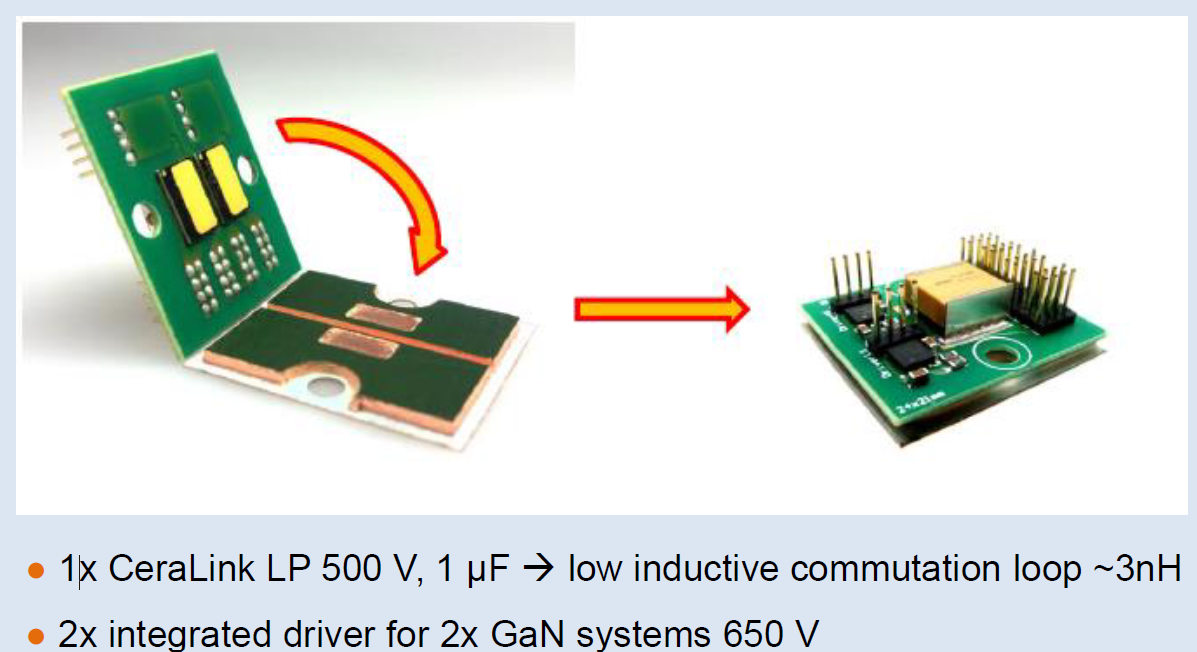
\includegraphics[width=\linewidth]{fig/lec08/GaN_integrated_DC_link.png}
    \caption{GaN power module with integrated driver and DC-link capacitors using low-inductance CeraLink placement. Adapted from TDK Electronics, \textit{Ceramic Capacitor Technology: CeraLink Opens New Dimensions in Power Electronics}}
\end{figure}
\end{column}
\end{columns}
The goal is not only low component ESL, but low total loop inductance from the capacitor to the switching cell.
\end{frame}


%%%%%%%%%%%%%%%%%%%%%%%%%%%%%%%%%%%%%%%%%%%%%%%%%%%%%%%%%%%%%
%% Final capacitor selection philosophy
%%%%%%%%%%%%%%%%%%%%%%%%%%%%%%%%%%%%%%%%%%%%%%%%%%%%%%%%%%%%%
\begin{frame}
\frametitle{Capacitor Selection Philosophy for Power Electronics}
\begin{columns}
\begin{column}{0.56\textwidth}
A good capacitor design is a multi-domain design. The designer must simultaneously satisfy:
\begin{itemize}
    \item required capacitance,
    \item voltage rating and derating,
    \item RMS ripple-current rating,
    \item peak-current and \(dv/dt\) rating,
    \item ESR and ESL limits,
    \item self-resonant frequency,
    \item thermal rise, lifetime and ageing,
    \item mechanical robustness,
    \item safety and discharge requirements,
    \item manufacturability and cost.
\end{itemize}

\end{column}

\begin{column}{0.40\textwidth}
\begin{center}
\begin{circuitikz}[scale=0.76, transform shape]
    \tikzstyle{block} = [draw, rounded corners, align=center,
    minimum width=2.45cm, minimum height=0.62cm, font=\scriptsize]

    \node[block] (cap) at (0,0) {Capacitor\\design};

    \node[block] (elec) at (-3.0,-1.4) {Electrical\\stress};
    \node[block] (therm) at (0,-1.4) {Thermal\\stress};
    \node[block] (mech) at (3.0,-1.4) {Mechanical\\stress};

    \node[block] (rel) at (-1.5,-3.0) {Reliability\\and lifetime};
    \node[block] (layout) at (1.5,-3.0) {Layout and\\parasitics};

    \draw[->, thick] (cap) -- (elec);
    \draw[->, thick] (cap) -- (therm);
    \draw[->, thick] (cap) -- (mech);
    \draw[->, thick] (elec) -- (rel);
    \draw[->, thick] (therm) -- (rel);
    \draw[->, thick] (mech) -- (rel);
    \draw[->, thick] (elec) -- (layout);
    \draw[->, thick] (layout) -- (rel);
\end{circuitikz}
\end{center}

\begin{block}{Message}
\small
A capacitor is not a passive afterthought. It is a converter-defining component.
\end{block}
\end{column}
\end{columns}
In modern converters, capacitor selection is inseparable from layout design, cooling design, and reliability design.
\end{frame}


%%%%%%%%%%%%%%%%%%%%%%%%%%%%%%%%%%%%%%%%%%%%%%%%%%%%%%%%%%%%%
%% Final summary
%%%%%%%%%%%%%%%%%%%%%%%%%%%%%%%%%%%%%%%%%%%%%%%%%%%%%%%%%%%%%
\begin{frame}
\frametitle{Summary: Capacitors in Power Electronics}
\begin{itemize}
    \item Capacitors store energy in electric fields and oppose changes in voltage.
    \item Ideal capacitor behaviour is described by: $i_C=C\frac{dv_C}{dt}, \qquad E_C=\frac{1}{2}CV^2$.
    \item Real capacitors contain ESR, ESL, leakage resistance, dielectric loss and dielectric absorption.
    \item Different converter positions require different capacitor technologies:
    input, output, DC-link, snubber, resonant, EMI and AC filter capacitors.
    \item Aluminum electrolytic capacitors provide high capacitance but are lifetime-limited by electrolyte ageing.
    \item Film capacitors provide low loss, high ripple capability and self-healing behaviour.
    \item MLCCs provide excellent high-frequency decoupling but require DC-bias, mechanical and cracking considerations.
    \item Capacitor sizing requires voltage, capacitance, ripple current, loss, temperature and lifetime checks.
    \item In SiC and GaN converters, low ESL, compact layout, high \(dv/dt\) capability and thermal robustness become decisive.
    \item Good capacitor design is an electro-thermal-reliability-layout co-design problem.
\end{itemize}

\end{frame} % Introduction to power module packaging, reliability, and testing, and thermal management
%\include{tex/dict} % English-German dictionary
\end{document} 